%
% ALEA ?
% ALEA ?
%
% On page 28 line -7, 2 \leq i \leq j \leq k ? 
% On page 28 line -7, 2 \leq i \leq j \leq k ? 
%
% On page 28 line -3, C(k,r) can be C(r) for the first term
% On page 28 line -3, C(k,r) can be C(r) for the first term
%
%
% Graphon <-> 1D disk binomial disk model with fixed number of points ? 
% Graphon <-> 1D disk binomial disk model with fixed number of points ? 
% Graphon <-> 1D disk binomial disk model with fixed number of points ? 
%
% Rand. Struct. Alg.
%
% Qte e.g. Grote, Julian; Thäle, Christoph Gaussian polytopes: a cumulant-based approach. J. Complexity 47 (2018), 1-41 + others. 
%
% Qte "On Connected Diagrams and Cumulants of Erdős-Rényi Matrix Models" by O. Khorunzhiy
%
% Use convolution of Moebius transforms as on page 21 of Peccati-Taqqu ? 
% Use convolution of Moebius transforms as on page 21 of Peccati-Taqqu ? 
%
%
% k-hop paths under the assumption that k - 1 < 1/r0 ≤ k. This assumption implies that it suffices to consider paths moving forward at each step (as any path with a backward step cannot reach 1 from 0 in k steps), which greatly simplifies the analysis.
%
% k is the smallest possible length of a path, i.e., the smallest integer such that k r_0>1.
%
% J. Stat. Phys
%
% Random Structures Algorithms
%
% J. Phys. A
%
% Phys. A
%
% Comb. Prob. Comp.
% 

\documentclass[12pt]{article}

\usepackage{amssymb,amsmath}
\usepackage[T1]{fontenc}

\usepackage{stackengine}

\usepackage{accents} 

\let\Horig\H

% \usepackage{amsfonts} 

\usepackage{dsfont}

% \usepackage[round]{natbib} 

% \usepackage{color}
\usepackage[usenames,dvipsnames,table]{xcolor}
% \usepackage{xcolor}
\definecolor{ForestGreen}{RGB}{34,139,34}
\definecolor{mauve}{rgb}{0.7,0,0.43}
\definecolor{dkgreen}{rgb}{0,0.6,0}
\definecolor{darkgreen}{rgb}{0,0.6,0}
\definecolor{darkorange}{rgb}{1.0, 0.55, 0.0}
\definecolor{lightblue}{rgb}{0,0.2,0.5}
\definecolor{blue1}{rgb}{0,0.1,0.9}

\definecolor{lightblue}{rgb}{0,0.2,0.5}

\usepackage[colorlinks=true, urlcolor=blue,linkcolor=blue, citecolor=lightblue]{hyperref}

\definecolor{codegreen}{rgb}{0,0.6,0}
\definecolor{codegray}{rgb}{0.5,0.5,0.5}
\definecolor{backcolour}{rgb}{0.97,0.97,0.97}

% \usepackage[round,sort,comma,numbers]{natbib}

% \bibpunct{\textcolor{lightblue}{(}}{\textcolor{lightblue}{)}}{,}{a}{}{;}

% \bibpunct{\textcolor{black}{(}}{\textcolor{black}{)}}{,}{a}{}{;}

% \usepackage{hyperref}

%%%% \let\oldcitet=\citet
%%%% \let\oldcitep=\citep 
%%%% \renewcommand{\cite}[1]{\textcolor[rgb]{0,0,1}{\oldcitet{#1}}}
%%%% \renewcommand{\citet}[1]{\textcolor[rgb]{0,0,1}{\oldcitet{#1}}}
%%%% \renewcommand{\citep}[1]{\textcolor[rgb]{0,0,1}{\oldcitep{#1}}}

\usepackage{caption}
\usepackage{subcaption}

\usepackage{tikz}

\usetikzlibrary{automata,topaths}
\usetikzlibrary{shapes}
\usetikzlibrary{plotmarks}

\usetikzlibrary{calc,shapes}

\usetikzlibrary{positioning, fit, shapes.geometric}

\usetikzlibrary{hobby,backgrounds,calc,trees}

\pgfdeclarelayer{background}
\pgfsetlayers{background,main}


\newcommand{\hobbyconvexpath}[2]{
[   
    create hobbyhullnodes/.code={
        \global\edef\namelist{#1}
        \foreach [count=\counter] \nodename in \namelist {
            \global\edef\numberofnodes{\counter}
            \node at (\nodename)
[draw=none,name=hobbyhullnode\counter] {};
        }
        \node at (hobbyhullnode\numberofnodes)
[name=hobbyhullnode0,draw=none] {};
        \pgfmathtruncatemacro\lastnumber{\numberofnodes+1}
        \node at (hobbyhullnode1)
[name=hobbyhullnode\lastnumber,draw=none] {};
    },
    create hobbyhullnodes
]
($(hobbyhullnode1)!#2!-90:(hobbyhullnode0)$)
\pgfextra{
  \gdef\hullpath{}
\foreach [
    evaluate=\currentnode as \previousnode using int(\currentnode-1),
    evaluate=\currentnode as \nextnode using int(\currentnode+1)
    ] \currentnode in {1,...,\numberofnodes} {
    \ifnum\currentnode=1\relax
    \xdef\hullpath{([closed=true]$(hobbyhullnode\currentnode)!#2!180:(hobbyhullnode\previousnode)$)
  ..($(hobbyhullnode\nextnode)!0.5!(hobbyhullnode\currentnode)$)}
    \else
    \xdef\hullpath{\hullpath
  ..($(hobbyhullnode\currentnode)!#2!180:(hobbyhullnode\previousnode)$)
  ..($(hobbyhullnode\nextnode)!0.5!(hobbyhullnode\currentnode)$)}
    \fi
    \ifx\currentnode\numberofnodes
    \else
    \xdef\hullpath{\hullpath
  ..($(hobbyhullnode\nextnode)!#2!-90:(hobbyhullnode\currentnode)$)}
    \fi
}
}
\hullpath
}

\usepackage{pgfplots}
\usepackage{wasysym} 

\usepackage{floatrow}
\DeclareFloatFont{footnotesize}{\footnotesize}% "scriptsize" is defined by floatrow, "tiny" not
\floatsetup[table]{font=footnotesize} 

\usepackage{float} 

% \usepackage{color} 
% \usepackage[colorlinks=true, urlcolor=blue,linkcolor=blue, citecolor=blue]{hyperref}
%%%% \usepackage[colorlinks=true, urlcolor=blue,linkcolor=blue, citecolor=black]{hyperref}
\DeclareMathAlphabet{\eufrak}{U}{}{}{} 
\SetMathAlphabet\eufrak{normal}{U}{euf}{m}{n}
\SetMathAlphabet\eufrak{bold}{U}{euf}{b}{n}

\numberwithin{equation}{section}

\newenvironment{Proof}{\removelastskip\par\medskip
\noindent{\em Proof.} \rm}{\penalty-20\null\hfill\huge$\square$\par\medbreak}

\newenvironment{Proofx}{\removelastskip\par\medskip
\noindent{\em Proof.} \rm}{\par}

\newenvironment{Proofy}{\removelastskip\par\medskip
\noindent{\em Proof} \rm}{\penalty-20\null\hfill$\square$\par\medbreak}

\allowdisplaybreaks

 \def\law{\rm Law} 
 \def\ci{\mathcal{I}} 
 \def\Pn{\rm Pn} 
 \def\cc{c} 
 \newcommand{\bone}{{\bf 1}}
 \newcommand{\cov}{\mathrm{Cov}}
\newcommand{\dtv}{{d_{\rm TV}}}
\newcommand{\dk}{{d_{\rm K}}}
\newcommand{\dw}{{d_{\rm W}}}
 \def\heta{{\eta}}
 \def\hp{{p}}
 \def\hh{{h}}
 \def\hH{{H}}
 \def\hPsi{{\Psi}}
 \def\hD{{D}}
 \def\complex{{\mathord{\mathbb C}}}
 \def\real{{\mathord{\mathbb R}}}
 \def\R{{\mathord{\mathbb R}}}
 \def\bbr{{\mathord{\mathbb R}}}
 \def\inte{{\mathord{\mathbb N}}}
 \def\z{{\mathord{\mathbb Z}}}
 \def\Z{{\mathord{\mathbb Z}}}
 \def\qu{{\mathord{\mathbb Z}}}
\def\erphi{1} 
\def\ind{{\bf 1}}
 \def\Cov{{\mathrm{{\rm Cov}}}}
 \def\Var{{\mathrm{{\rm Var}}}}
 \def\Dom{{\mathrm{{\rm Dom}}}}
 \def\trace{{\mathrm{{\rm trace}}}}
 \def\id{{\mathrm{{\rm Id}}}}
 \def\Ent{{\mathrm{{\rm Ent}}}}
 \def\var{{\mathrm{{\rm var}}}}
% \def\div{{\mathrm{{\rm div}}}}
 \def\Diff{{\mathrm{{\rm Diff}}}}
 \def\T{{\mathrm{{\rm T}}}}
 \def\real{{\mathord{{\rm I\kern-3pt R}}}}        % Fake blackboard bold R.
 \def\G{{\mathord{{\rm {\sf G}}}}}
 \def\inte{{\mathord{{\rm I\kern-3pt N}}}}
 \def\sZZ{{\rm Z\kern-.45em{}Z}}
%\def\z{\sZZ} 
%\def\z{{\mathchoice {\sZZ} {\sZZ} {\rm Z\kern-0.30em{}Z} {\rm Z\kern-0.25em{}Z} }}
 \def\sQQ{{\kern 0.27em \vrule height1.45ex width0.03em depth0em
           \kern-0.30em \rm Q}}
 \def\qu{{\mathchoice
         {\sQQ}
         {\sQQ}
   {\kern 0.225em \vrule height1.05ex width0.025em depth0em \kern-0.25em \rm Q}
   {\kern 0.180em \vrule height0.78ex width0.020em depth0em \kern-0.20em \rm Q}
         }}
 \def\sGG{{\kern 0.27em \vrule height1.45ex width0.03em depth0em
           \kern-0.30em \rm G}}
% \def\gg{{\mathchoice
%         {\sGG}
%         {\sGG}
%   {\kern 0.225em \vrule height1.05ex width0.025em depth0em \kern-0.25em \rm G}
%   {\kern 0.180em \vrule height0.78ex width0.020em depth0em \kern-0.20em \rm G}
%         }}

 \newtheorem{prop}{Proposition}[section]
 \newtheorem{lemma}[prop]{Lemma}
 \newtheorem{definition}[prop]{Definition}
 \newtheorem{corollary}[prop]{Corollary}
 \newtheorem{theorem}[prop]{Theorem}
 \newtheorem{remark}[prop]{Remark}
 \newtheorem{example}[prop]{Example}

\newtheorem{assumption}{Assumption}[section]
 
 \def\Dom{{\mathrm{{\rm Dom \! \ }}}}
% \def\IP{{\mathord{\mathbb P}}}
 \def\trace{{\mathrm{{\rm trace}}}}
 \def\Ent{{\mathrm{{\rm Ent}}}}
 \def\var{{\mathrm{{\rm var}}}}
% \def\div{{\mathrm{{\rm div}}}}

\def\E{\mathop{\hbox{\rm I\kern-0.20em E}}\nolimits}
\def\P{\mathop{\hbox{\rm I\kern-0.20em P}}\nolimits}
% \def\P{{\mathord{\mathbb P}}}

\newcommand{\unit}{\mbox{\boldmath $1$}}
\newcommand{\nor}{\mbox{$\gamma (K)$}} 
\newcommand{\dee}{\mbox{$I  \! \! \! \, D$}}
\newcommand{\lee}{\mbox{$I  \! \! \! \, L$}}

\def\card{{\mathord{{\rm card}}}}

 \newcounter{hyp}
 \setcounter{hyp}{0}

 \textwidth16.3cm
 \textheight21.5cm
 \oddsidemargin0.2cm
 \evensidemargin0.2cm
 \topmargin0.8cm
 \headheight0cm
 \headsep0cm
 \baselineskip1in
 %\parindent0.5in
 \parindent0.25in
 \renewcommand{\thefootnote}{\fnsymbol{footnote}}

\usepackage{textcomp}

\usepackage{accsupp}    

 \newcommand{\noncopynumber}[1]{
    \BeginAccSupp{method=escape,ActualText={}}
    #1
    \EndAccSupp{}
}
 
\usepackage{listings}
\lstset{ % 
  xleftmargin=14pt, % 3.4pt,
  xrightmargin=3.4pt,
  language=[5.2]Mathematica,                % the language of the code 
  basicstyle=\scriptsize\ttfamily, % \tiny\ttfamily, % \footnotesize,           % the size of the fonts that are used for the code 
%  basicstyle=\ttfamily,
  numbers=left, % none,                   % where to put the line-numbers
  numberstyle=\tiny\color{gray}\noncopynumber,  % the style that is used for the line-numbers 
% firstnumber=1,
 stepnumber=2,                   % the step between two line-numbers. If it's 1, each line 
                                  % will be numbered 
  numbersep=5pt,                  % how far the line-numbers are from the code 
  backgroundcolor=\color{backcolour},      % choose the background color. You must add \usepackage{color} 
  showspaces=false,               % show spaces adding particular underscores 
  showstringspaces=false,         % underline spaces within strings 
  showtabs=false,                 % show tabs within strings adding particular underscores 
  frame=single,                   % adds a frame around the code 
  rulecolor=\color{black},        % if not set, the frame-color may be changed on line-breaks within not-black text (e.g. commens (green here)) 
  tabsize=2,                      % sets default tabsize to 2 spaces 
  captionpos=b,                   % sets the caption-position to bottom 
  breaklines=true,                % sets automatic line breaking 
  breakatwhitespace=true,        % sets if automatic breaks should only happen at whitespace 
  title=\lstname,                   % show the filename of files included with \lstinputlisting; 
                                  % also try caption instead of title 
  keywordstyle=\color{blue1},          % keyword style 
  commentstyle=\color{dkgreen},       % comment style 
  stringstyle=\color{mauve},         % string literal style 
  escapeinside={\%*}{*)},            % if you want to add a comment within your code 
  morekeywords={*,...},               % if you want to add more keywords to the set 
  columns=fullflexible,
  upquote
}

\newcommand{\re}{\mathrm{e}}            % Roman e for exponential

\title{\Large \textcolor{red}{Phase Transitions for $k$-Hop Connectivity in One-Dimensional Binomial Random-Connection Models}}
 
\date{\normalsize \today} 
%\today 


\author{
  Qingwei Liu\footnote{
School of Mathematics and Statistics, The University of Melbourne, Parkville, VIC 3010, Australia. 
Email: \href{mailto:qingwei.liu@unimelb.edu.au}{qingwei.liu@unimelb.edu.au}}
  % Department of Statistics and Data Science, National University of Singapore, 6 Science Drive 2, Singapore 117546,
% Email: \href{mailto:liu\_qw@nus.edu.sg}{liu\_qw@nus.edu.sg}}
%  Email: \href{mailto:xiaozong30@gmail.com}{xiaozong30@gmail.com}}
  \qquad
  Nicolas Privault\footnote{%Division of Mathematical Sciences,
School of Physical and Mathematical Sciences, Nanyang Technological University, 21 Nanyang Link, Singapore 637371. Email: \href{mailto:nprivault@ntu.edu.sg}{nprivault@ntu.edu.sg}
}
}
      %\author{ } 

% \citationstyle{chicago} 

\DeclareMathSymbol{\mlq}{\mathord}{operators}{``}
\DeclareMathSymbol{\mrq}{\mathord}{operators}{`'}

\let\savering\ring
\let\saveleftmoon\leftmoon
\let\saverightmoon\rightmoon
\let\savefullmoon\fullmoon
\let\savenewmoon\newmoon
\let\savediameter\diameter
\let\ring\relax
\let\leftmoon\relax
\let\rightmoon\relax
\let\fullmoon\relax
\let\newmoon\relax
\let\diameter\relax
\usepackage{mathabx}
\let\ring\savering
\let\leftmoon\saveleftmoon
\let\rightmoon\saverightmoon
\let\fullmoon\savefullmoon
\let\newmoon\savenewmoon
\let\diameter\savediameter

% \usepackage{tabularx} 
\usepackage{nicematrix}
\usepackage{hhline} 

\usepackage{enumerate} 

% \usepackage{refcheck}

\hyphenation{func-tio-nals} 
\hyphenation{Privault} 

\begin{document}

\setlength\arrayrulewidth{0.6pt}

\hyphenation{func-tio-nals} 
\hyphenation{Privault} 

\maketitle 

\vspace{-0.8cm}

\baselineskip0.6cm
 
\begin{abstract} 
\textcolor{red}{
We study the number of $k$-hop paths between two fixed endpoints in a one-dimensional binomial random-connection model. By deriving explicit combinatorial expressions for the joint moments of all orders, we analyze the asymptotic growth of cumulants as the number of points in the underlying point process tends to infinity. We show that, depending on the scaling regime, the $k$-hop count exhibits a phase transition between Gaussian and Poisson limits. 
Moreover, we establish both a central limit theorem with explicit convergence rates under the Kolmogorov distance and quantitative Poisson approximation bounds. These results provide a detailed description of the  fluctuation behavior for multi-hop connectivity in one-dimensional random-connection models.}
%  We derive moment identities and cumulant bounds for
%  the count of $k$-hops in a one-dimensional binomial
%  random-connection model with unit disk connection function.
%  Normal and Poisson approximation results with quantitative rate
%  estimates are then obtained for $k$-hop counts.
\end{abstract} 
 
\noindent {\bf Key words:} 
\textcolor{red}{Random-connection model, 
Phase transition,
Central limit theorem,
Poisson approximation,
Multi-hop connectivity,
Cumulants and joint moments.}
%Random graph,
%1D unit disk model,
%$k$-hop counts, 
%binomial process,
%Poissonization,
% multiple stochastic integrals,
%moments,
%cumulants. 
\\ 
{\em Mathematics Subject Classification (2020):} 
05C80, % Random graphs (graph-theoretic aspects)
60G55, % Point processes (e.g., Poisson, Cox, Hawkes processes)
% 60G57	Random measures
60F05, % Central limit and other weak theorems
\textcolor{red}{60D05}. % Geometric probability and stochastic geometry 
 
\baselineskip0.7cm
 
\section{Introduction}
\noindent
Random-connection models (RCMs) are random graphs based on
randomly located vertices which are independently connected
with a location-dependent probability. 
 They include the binomial RCM 
 which can be regarded as 
 a generalization of the Erd{\H o}s-R\'enyi model, 
 and has been studied under different names, for example
 as inhomogeneous random graphs,
 c.f. \cite{DevroyeFraiman14,penrose18,hladky21}, and as
 graphon-based random graphs c.f. \cite{coulson16,zhangzs,bhattacharya23}.

 \medskip

 In this paper, we focus on the one-dimensional 
 unit disk binomial RCM with connection radius $r>0$
 on a finite interval, see \cite{drory1997},
 as illustrated Figure~\ref{fjkld23}.  
 \textcolor{red}{Specifically, we investigate the number of paths of length $k$ (or $k$-hop paths) connecting two fixed endpoints. Multi-hop connectivity is a critical metric in applications such as wireless networks, device-to-device and/or station-to-device communications in cellular networks and spread of infection.}
%   \vspace{-11cm}
 \begin{figure}[H]
   \begin{center}
   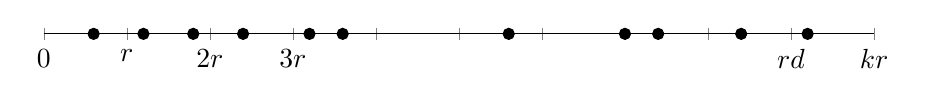
\begin{tikzpicture}
   \begin{axis}[
       height=2cm,
       xmin=0, xmax=50,
    width=1\textwidth,
    axis x line=bottom,% only show the bottom x axis
    axis line style={-},
    hide y axis,    
    ymin=0,ymax=5,
    xticklabels={0,0,$r$,$2r$,$3r$,,,,,,$rd$,$kr$},
    scatter/classes={%
        a={mark=o,draw=black}}
    ]

\addplot[scatter,only marks,
    mark size = 2pt,
    fill = black,
    scatter src=explicit symbolic]
table {
3 0 
6 0 
9 0 
12 0 
16 0 
18 0 
28 0 
35 0 
37 0 
42 0 
46 0 
58 0 
    };
\end{axis}

\end{tikzpicture}
\end{center}
   \vskip-0.4cm
%   \caption{Unit disk random-connection model.}
   \caption{Binomial point process.} 
   \label{fjkld23}
 \end{figure}
 
   \vskip-0.3cm

   \noindent
% \noindent
   \textcolor{red}{We consider nodes distributed over the interval $[0, kr]$, where $k \geq 2$, according to a binomial point process $\eta$ constrained to have $m_i$ points within each cell $[(i-1)r, ir]$, $i=1, \ldots, k-1$. We assume a connection probability $p \in [0,1]$ such that any two nodes at locations $s$ and $t$ are connected if and only if $|t-s| \leq r$. In this setting, a $k$-hop path is defined as a sequence connecting two fixed endpoints $s, t \in [0, kr]$ through exactly $d:=k-1$ intermediate nodes.}
 \medskip

% \noindent
 \textcolor{red}{We investigate the random variable $\sigma_k(t)$, defined as the number of $k$-hop paths connecting two fixed endpoints located at $0$ and $t \in [0, kr]$. The exact distribution of these counts was previously derived using a combinatorial approach in \cite{giles-privault}. In the present work, we analyze the asymptotic behavior of $\sigma_k(t)$ as the number of points in the underlying binomial process tends to infinity. To this end, we employ the method of cumulants, see \cite{rudzkis, saulis, doring, thale18, doering}. This method has been successfully applied recently to study moderate deviations in random geometric graphs and weighted random-connection models \cite{schulte-thaele, heerten}, as well as normal approximations for subgraph counts in multidimensional random-connection models \cite{LiuPrivault}, including settings with fixed endpoints \cite{LiuPrivault24}.}
 %We are interested in the count $\sigma_k ( t )$ of  $k$-hops connecting two fixed endpoints located respectively at $0$ and $t$ for some $t \in [0,kr]$. In this context, the distribution of $k$-hop counts has been expressed by a combinatorial approach in \cite{giles-privault}. We will consider the asymptotic behavior of the count statistics $\sigma_k (t)$ as the number of binomial points tends to infinity.
% When $k=1$ we have $\sigma_1(t) =1$, $t\in [0,r]$. 
 % where for later convenience of notation we model $\sigma_k$ as a function of the remaining distance $kr-\tau$ from $t$ to $kr$. For this, we will use the cumulant method, see \cite{rudzkis}, \cite{saulis},
 %\cite{khorunzhiy},
 %\cite{doring},
 %\cite{thale18},
% \cite{jansen},
 %\cite{doering},
 %which has been recently applied
 %to moderate deviation in random geometric graphs
 %and weighted random-connection models 
 %in \cite{schulte-thaele}, \cite{heerten}, 
 %and to normal approximation for subgraph counts
 %in the multidimensional random-connection model, 
 %see \cite{LiuPrivault}, and \cite{LiuPrivault24} in the presence of endpoints.  

 \medskip
 
 In Proposition~\ref{p1}, 
 we derive a combinatorial expression for
 the joint moments 
 of $k$-hop counts \textcolor{red}{corresponding to } different endpoint locations within $[rd,rk]$.
 \textcolor{red}{We then specialize this general result in Proposition~\ref{djklfs2} and Corollary~\ref{djklfs2-2} to obtain explicit formulas for the variance.}

\medskip
\textcolor{red}{Subsequently, we focus on the homogeneous case where $m_1=m_2=\cdots=m_d=m \geq 1$. Let $\P_m$ denote  
the distribution of the one-dimensional unit disk model with $m$ points per cell and connection probability $p_m$. 
We also denote by $\kappa_n\big(\widebar{\sigma}_k (t)\big)$ the cumulant of order 
$n\geq 2$ of the normalized $k$-hop count
$$ 
   \widebar{\sigma}_k (t):= \frac{\sigma_k (t)-\E_m [ \sigma_k (t)]}{\sqrt{\Var_m [ \sigma_k (t) ]}}. 
$$ 
In Section~\ref{sec6}, we first derive a general 
cumulant bound for $\sigma_k(t)$; see Theorem~\ref{jkldd12}. This leads to a refined 
estimation in Theorem~\ref{th7.5-1} depending on the connection probability $p_m$. 
Combining this with the asymptotic variance established in Proposition~\ref{prop7.6}, 
we obtain the following bound in Corollary~\ref{cjkfl} 
\begin{equation*}
    \kappa_n\big(\widebar{\sigma}_k (t)\big)\leq \begin{cases}
      \displaystyle
      \frac{n!^{d+1}}{(C m p_m)^{n/2-1}} & \text{when } p_m \gg m^{-(d-1)/d},
      \medskip
      \\
      \displaystyle
      \frac{n!^{d+1}}{\big(C m^d p_m^{d+1}\big)^{n/2-1}} & \text{when } p_m\ll m^{-1},
    \end{cases}
\end{equation*}
for $n\ge3$, where $C$ is a constant independent of $m \geq 1$.}
  \medskip

\textcolor{red}{This moment--cumulant analysis reveals a phase transition between Gaussian and 
Poisson limiting regimes under different scalings. Using the method of cumulants, 
we obtain in Corollary~\ref{thm4.2-1} the bound \eqref{fjkf} for the convergence 
of the normalized $k$-hop count $\widebar{\sigma}_k (t)$ to the standard normal 
distribution under the Kolmogorov distance as $m$ tends to infinity. Furthermore, 
in Theorem~\ref{poi-thm}, we provide a Poisson approximation for the $k$-hop 
count via the Stein-Chen method.}

\medskip
We employ the following standard notation for the asymptotic behavior of functions 
$f(x)$ and $g(x)>0$ as $x$ tends to infinity.
We write 
\begin{itemize}
\item $f(x)=O(g(x))$, or $f(x) \lesssim g(x)$, if $\limsup_{x\to\infty} f(x) / g(x) <\infty$,
\item $f(x)=\Omega(g(x))$, or $f(x) \gtrsim g(x)$, if $\liminf_{x\to\infty} f(x) / g(x)>0$,
\item $f(x)\asymp g(x)$ if $f(x)=O(g(x))$ and $f(x)=\Omega(g(x))$, % if $f(\lambda )=\Theta(g(\lambda ))$;
\item $f(x)\sim g(x)$ if $\lim_{x \to \infty} f(x)/g(x) = 1$, 
\item $f(x)\ll g(x)$, or $g(x)\gg f(x)$, if $f(x)\geq 0$ and $f(x)/g(x)\to 0$.
\end{itemize}
with the convention $0/0=0$. 
\textcolor{red}{Throughout, we denote by $\Phi$ the cumulative distribution function of the standard normal distribution. For $d\geq 2$ and a fixed endpoint $t\in [(k-1)r,kr]$, we identify the following three regimes:}
\begin{description}
	\item[Dense regime.]
  If $p_m \gg m^{-1+1/d}$,
    then we have $\lim_{m\to\infty}\P_m (\sigma_k (t) \geq 1)=1$,
    see Corollary~\ref{graphcontain}-$a)$. Moreover, the normalized count satisfies the Kolmogorov bound 
    \begin{equation}
   \nonumber % \label{fjkf}
   \sup_{x\in\real }|\P_m (\widebar{\sigma}_k (t)\leq x)-\Phi(x)|
 \leq \frac{C_d}{(m p_m)^{1/(2+4d)}},
    \end{equation}
    for $m$ large enough, 
    where $C_d>0$ depends only on
    $d \geq 2$, see 
    Corollary~\ref{thm4.2-1}.
\item[Thermodynamic regime.]
    If $p_m \asymp m^{-1+1/d}$, 
    then as $m$ tends to infinity we have
\begin{align}
	\dtv(\sigma_k (t),\Pn(\lambda\textcolor{red}{(t)}))&
  \asymp \frac{1}{m^{1/(d+1)}},
\nonumber % \label{po-error1}
\end{align}
where \textcolor{red}{$\Pn(\lambda)$ denotes the Poisson distribution with parameter $\lambda$, $\lambda(t)=\E_m[\sigma_k(t)]$} and $\dtv$ is the total variation distance; 
see Corollary~\ref{c2} and \eqref{dtv}.
\item[Sparse regime.]
  If $p_m\ll m^{-1}$, we have the convergence in probability 
  $$
  \lim_{m\to\infty}\P_m (\sigma_k (t) =0)=1,
  $$
 see Corollary~\ref{graphcontain}-$b)$. 
\end{description}
    % In Proposition~\ref{fsklf34} we also obtain the Berry-Esseen bound
% $$\sup_{x\in \real} | \P_m ( \widebar{\sigma}_k (t) \leq x ) - \P_m ({\cal N} \leq x ) | \leq \frac{C(k,r)}{\sqrt{m}} $$ using the Stein method, together with a bound of same order for the Wasserstein distance.
% In Theorem~\ref{poi-thm}, we provide a Poisson approximation of the $k$-hop count via Stein-Chen method. In particular, when $m^dp_m^{d+1}\to c\in(0,\infty)$, in Corollary~\ref{c2} we show that the error bound for the Poisson approximation is of the order  
%\begin{align} \dtv(W,\Pn(\lambda))&  \asymp m^{-1/(d+1)}.\nonumber % \label{po-error1}\end{align}as $m_1=m_2=\cdots=m_d=m$ tends to infinity.
% \medskip 
The paper is organized as follows. Section~\ref{sec3} formulates the $k$-hop count within the framework of generalized $U$-statistics. Section~\ref{sec-prel} introduces the necessary preliminaries on diagrams and set partitions, which lay the groundwork for Section~\ref{sec4}, where we express the moments as summations over non-crossing partitions.  In Section~\ref{sec6}, we derive explicit bounds for moments and cumulants, which leads to a normal approximation for the normalized $k$-hop counts with Berry--Esseen rates via the Stein and cumulant methods in Section~\ref{sec8}. Finally, Section~\ref{sec-pol} provides a Poisson approximation using the Stein--Chen method.

\section{Binomial model and $k$-hop counts} 
% \label{sec4}
% \section{Single node per cell} 
\label{sec3}
\subsubsection*{$U$-Statistics formulation} 
\noindent
For $r>0$, $k\ge2$, let $J_\ell:=[(\ell-1)r,\ell r]$ denote some intervals with equal length, $\ell=1,\dots,k$, referred as {\em cells}.
For each $\ell=1,\dots,d$, let $\tilde{\mu}_\ell$ be a non-atomic probability measure concentrated on $J_\ell$.
For each $\ell=1,\dots,d$,
let $\{X^{(\ell)}_i\}_{i=1}^{m_\ell}$, $m_\ell\ge1$,
be a sequence of i.i.d. random variables with a common distribution $\tilde{\mu}_\ell$, and independent of all others.
Denote 
$$\mathcal{P}:=
\{0,t\}
\bigcup
\bigcup_{\ell=1}^{d}\left\{X^{(\ell)}_{1},\dots,X^{(\ell)}_{m_\ell}\right\},
$$ 
 with $t\in ((k-1)r,kr)$. %  for some $\tau\in(0,r)$.

In this article, we consider a random graph, also referred as a random connection model, constructed as follows.
For any two distinct points $u,w\in\mathcal{P}$, if $|u-w|\le r$, then they are connected by a random edge with probability $p\in[0,1]$ independently, denoted by $u\leftrightarrow w$.
Let the resulting random graph be denoted by $\mathbb{G}_p(\mathcal{P})$.

We focus on the count of $k$-hop, that is a path of order $k+1$, connecting $0$ to $t$ in the random connection model $\mathbb{G}_p(\mathcal{P})$.
More formally, we can write it as 
\begin{equation}
  \nonumber 
	\sigma_k (t):=\sum_{\beta\in[m_1]\times\cdots\times[m_{d}]}\bone(0\leftrightarrow X_{\beta(1)}^{(1)})\left(\prod_{\ell=1}^{k-2}\bone\left(X_{\beta(\ell)}^{(\ell)}\leftrightarrow X_{\beta(\ell+1)}^{(\ell+1)}\right)\right)\bone(X_{\beta(d)}^{(d)}\leftrightarrow t),\label{def-khop1}
\end{equation}
with $[n]:=\{1,2,\dots,n\}$.
 
 As noted in e.g. \cite{giles-privault}, when $t\in [(k-1)r,kr]$,
any node contributing to a $k$-hop path linking $0$ to $t$
must belong to one of the $d$ lenses pictured in pink in Figure~\ref{fklds},
and defined as the intervals
$$
L_i := [ir-\tau,ir] = [0,\tau] + ir - \tau, \qquad i=1,\ldots , d, 
$$ 
 of identical length $\tau : = kr - t$.

 \medskip


\begin{figure}[H]
\centering
\includegraphics[width=0.94\linewidth]{kops_new-crop}
\caption{Graph of seven $5$-hop paths linking $x=0$ to $t=4.5$ with $r=1$ and $d=4$.} 
\label{fklds} 
\end{figure}


\vskip-0.4cm

\noindent
 Conversely, any $k$-hop path linking $0$ to $t$
 should have exactly one 
 node in each cell $[(i-1)r,ir]$, $i=1,\ldots , d$.
 Therefore, it must be realized using a sequence 
 $(x_1, \ldots , x_d)$ of nodes,  such that
 $$
 x_{i+1} \leq x_i + r, \qquad i = 0,1,\dots, d,
 $$
 where $x_0=0$ and $x_k=t$.  
% \subsubsection*{One-dimensional random geometric graphs} 
% \label{s2}
Therefore, it can be mapped to a
 sequence $(y_1,\ldots , y_d) \in [0,kr-t]^d$
 by the relation 
 $$
 y_i:=x_i + ((k-i)r-t), \qquad i =1,\ldots , d, 
 $$ 
 with $ y_1 \ge \cdots \ge y_d$. 

 Hence, for $t\in [(k-1)r,kr]$, the count $\sigma_k (t)$ in \eqref{def-khop1} of $k$-hop 
 connecting $0$ to $t$ can be rewritten as a generalized $U$-statistics of order $d$
\begin{equation}
\label{ustat} 
 \sigma_k (t) = \sum_{\beta \in [m_1] \times \cdots \times [m_d]} 
 Y^{(0)}_{\beta (1)}Y^{(1)}_{\beta (1),\beta (2)}\cdots Y^{(d-1)}_{\beta (d-1),\beta (d)}
 Y^{(d)}_{\beta (d)}
 {\bf1}_{\big\{U^{(d)}_{\beta (d)} \leq \cdots \leq U^{(1)}_{\beta (1)} \leq kr-t \big\}},
\end{equation}
where
$$
\left\{
 Y^{(0)}_{\beta (1)}
 ,
 Y^{(1)}_{\beta (1),\beta (2)},
 \ldots ,
 Y^{(d-1)}_{\beta (d-1),\beta (d)}, 
 Y^{(d)}_{\beta (d)}:~\beta(i)\in[m_i], i=1,\dots,d\right\}
 $$
 is a family of independent % $\{0,1\}$-valued
 Bernoulli random variables with same parameter $p\in [0,1]$, where 
 $$
 U^{(\ell)}_{i}:=X^{(\ell)}_{i}-(t - (k-\ell) r ),
 $$
for $i=1,\dots,m_\ell$ and $\ell=1,\dots,d$. 
 From now on, we denote by $\mu_{\ell}:=\tilde{\mu}_\ell * \delta_{-( t - (k-\ell )r )}$, 
 the distribution of $U^{(\ell)}_i$ on $[0,r]$,
 for $i=1,\dots,m_\ell$ and $\ell=1,\dots,d$.

 \medskip
 
 Note that for $k=2$, $p=1$ and $t=k-1$, we have $\sigma_2 (r) =m_1$ almost surely.

\section{Set partitions and diagrams}\label{sec-prel}
\noindent
% We recall the following notation, see for example \cite{peccatitaqqu,LiuPrivault}.
 In what follows, we % let $[n]:=\{1,2,\dots,n\}$ for $n\geq 1$, and
 let $\Pi(b)$ denote the collection of set partitions of
any finite set $b$.
 Given two set partitions $\rho_1, \rho_2\in\Pi(b)$, we say that $\rho_1$ is
coarser than $\rho_2$
 (i.e. $\rho_2$ is finer than $\rho_1$), 
 and we write $\rho_2\preceq\rho_1$, 
if and only if each block of $\rho_2$ is contained in a block of $\rho_1$.
We use $\rho_1\vee\rho_2$ for the
finest partition which is coarser than both $\rho_1$ and $\rho_2$, and
denote by $\rho_1\wedge\rho_2$ the coarsest partition
which is finer than both of $\rho_1$ and $\rho_2$. We also let $\widehat{1}:=\{b\}$ 
denote the single-block coarsest partition of $b$,
 whereas $\widehat{0}$ stands for the partition made of singletons. 
 Given $k\geq 2$ and $n\geq 1$,
 we let $\pi:=\{\pi_1,\dots,\pi_n\}$ % \in\Pi([n]\times[d])$
 denote the partition
 of $[n]\times[d]$ defined as 
 $$\pi_i:=\{(i,\ell):1\leq \ell\leq d\},
 \quad i =1,\dots , n.
 $$
 For $k,n \geq 1$ we also let $\pi_\eta := (\pi_i)_{i\in\eta}\in\Pi(\eta \times [d])$ denote the partition made of $|\eta|$ blocks of size $d$.
 A partition $\rho\in\Pi([n]\times[d])$ is said to be {\it connected} if $\rho\vee\pi=\widehat{1}$, see Figure~\ref{fig:diagram0-1}.  

 % \vspace{-0.3cm}

 \begin{figure}[H]
\captionsetup[subfigure]{font=footnotesize}
\centering
\subcaptionbox{Connected partition.}[.49\textwidth]{
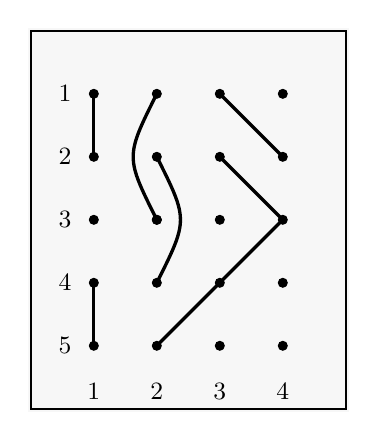
\begin{tikzpicture}[scale=0.8] 
\draw[black, thick] (0,0) rectangle (5,6);
\node[anchor=east,font=\small] at (0.8,5) {1};
\node[anchor=east,font=\small] at (0.8,4) {2};
\node[anchor=east,font=\small] at (0.8,3) {3};
\node[anchor=east,font=\small] at (0.8,2) {4};
\node[anchor=east,font=\small] at (0.8,1) {5};
\node[anchor=south,font=\small] at (1,0) {1};
\node[anchor=south,font=\small] at (2,0) {2};
\node[anchor=south,font=\small] at (3,0) {3};
\node[anchor=south,font=\small] at (4,0) {4};
\filldraw [black] (1,1) circle (2pt);
\filldraw [black] (2,1) circle (2pt);
\filldraw [black] (3,1) circle (2pt);
\filldraw [black] (4,1) circle (2pt);
\filldraw [black] (1,2) circle (2pt);
\filldraw [black] (2,2) circle (2pt);
\filldraw [black] (3,2) circle (2pt);
\filldraw [black] (4,2) circle (2pt);
\filldraw [black] (1,3) circle (2pt);
\filldraw [black] (2,3) circle (2pt);
\filldraw [black] (3,3) circle (2pt);
\filldraw [black] (4,3) circle (2pt);
\filldraw [black] (2,3) circle (2pt);
\filldraw [black] (1,4) circle (2pt);
\filldraw [black] (2,4) circle (2pt);
\filldraw [black] (3,4) circle (2pt);
\filldraw [black] (4,4) circle (2pt);
\filldraw [black] (1,5) circle (2pt);
\filldraw [black] (2,5) circle (2pt);
\filldraw [black] (3,5) circle (2pt);
\filldraw [black] (4,5) circle (2pt);
\draw[very thick] (1,5) -- (1,4); 
\draw[very thick] (3,5) -- (4,4);
\draw[very thick] (1,2) -- (1,1);
\draw[very thick] (2,2) .. controls (2.5,3) .. (2,4);
\draw[very thick] (2,3) .. controls (1.5,4) .. (2,5);
% \draw[very thick] (2,2) -- (2,4);
\draw[very thick] (2,1) -- (3,2) -- (4,3) -- (3,4);
  \begin{pgfonlayer}{background}
    \filldraw [line width=4mm,black!3]
      (0.2,0.2)  rectangle (4.8,5.8);
  \end{pgfonlayer}
\end{tikzpicture}}
\subcaptionbox{Non-connected partition.}[0.49\textwidth]{
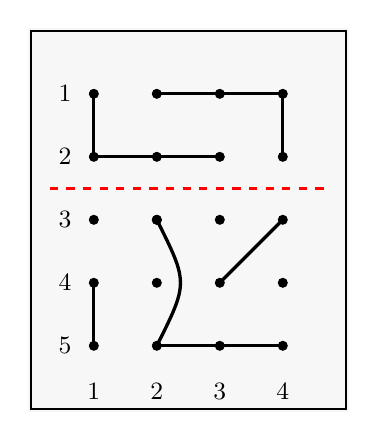
\begin{tikzpicture}[scale=0.8] 
\draw[very thick,dashed,red] (0.3,3.5) -- (4.7,3.5);
\draw[black, thick] (0,0) rectangle (5,6);
\node[anchor=east,font=\small] at (0.8,5) {1};
\node[anchor=east,font=\small] at (0.8,4) {2};
\node[anchor=east,font=\small] at (0.8,3) {3};
\node[anchor=east,font=\small] at (0.8,2) {4};
\node[anchor=east,font=\small] at (0.8,1) {5};
\node[anchor=south,font=\small] at (1,0) {1};
\node[anchor=south,font=\small] at (2,0) {2};
\node[anchor=south,font=\small] at (3,0) {3};
\node[anchor=south,font=\small] at (4,0) {4};
\filldraw [black] (1,1) circle (2pt);
\filldraw [black] (2,1) circle (2pt);
\filldraw [black] (3,1) circle (2pt);
\filldraw [black] (4,1) circle (2pt);
\filldraw [black] (1,2) circle (2pt);
\filldraw [black] (2,2) circle (2pt);
\filldraw [black] (3,2) circle (2pt);
\filldraw [black] (4,2) circle (2pt);
\filldraw [black] (1,3) circle (2pt);
\filldraw [black] (2,3) circle (2pt);
\filldraw [black] (3,3) circle (2pt);
\filldraw [black] (4,3) circle (2pt);
\filldraw [black] (2,3) circle (2pt);
\filldraw [black] (1,4) circle (2pt);
\filldraw [black] (2,4) circle (2pt);
\filldraw [black] (3,4) circle (2pt);
\filldraw [black] (4,4) circle (2pt);
\filldraw [black] (1,5) circle (2pt);
\filldraw [black] (2,5) circle (2pt);
\filldraw [black] (3,5) circle (2pt);
\filldraw [black] (4,5) circle (2pt);
\draw[very thick] (1,5) -- (1,4) -- (2,4) -- (3,4);
\draw[very thick] (2,5) -- (3,5) -- (4,5) -- (4,4);
\draw[very thick] (1,2) -- (1,1);
\draw[very thick] (2,1) .. controls (2.5,2) .. (2,3);
% \draw[very thick] (2,2) .. controls (1.5,3) .. (2,4);
% \draw[very thick] (2,3) -- (2,2);
\draw[very thick] (2,1) -- (3,1) -- (4,1);
\draw[very thick] (3,2) -- (4,3);
  \begin{pgfonlayer}{background}
    \filldraw [line width=4mm,black!3]
      (0.2,0.2)  rectangle (4.8,5.8);
  \end{pgfonlayer}
\end{tikzpicture}}
\caption{Examples of partition diagrams with $n=5$ and $d=4$.}
\label{fig:diagram0-1}
\end{figure}
 
 \vspace{-.4cm}
  
\noindent 
 We let $\Pi_{\widehat{1}}([n]\times[d])$ denote the collection of all
 connected partitions of $[n]\times[d]$. 
\begin{definition}
 We let ${\rm NC} ([n]\times [d])$ 
 denote the set of all partitions $\pi$ in $\Pi ([n]\times [d])$  
 that are non-crossing in the sense that
 if $(k,l)$ and $(k',l')$ belong to a same block of $\pi$ then we should have $l=l'$.
 \end{definition} 
 We also denote by 
 ${\rm CNC}([n]\times [d])$
  the set of all connected and non-crossing partitions of $[n]\times [d]$, for $n,k\geq 1$. 
 In what follows, every non-crossing partition $\rho$ of
 $[n]\times [d]$ will be decomposed as 
 \begin{equation}
   \label{fjklds143} 
 \rho = \bigcup_{i=1}^d \rho_i
\end{equation} 
 where $\rho_i$ is a partition of $\{(\ell ,i)\}_{\ell =1,\ldots , n}$
 for $i=1,\ldots , d$, 
% As above, we let $\lambda_l(s):=\lambda ( s)$, $l=1,\ldots , d$. 
 see Figure~\ref{fig:diagram0-1-2}\textcolor{red}{-(b)}.  
% \vspace{-0.3cm}
\begin{figure}[H]
\captionsetup[subfigure]{font=footnotesize}
\centering
\subcaptionbox{Crossing % non-flat
   partition.}[.49\textwidth]{
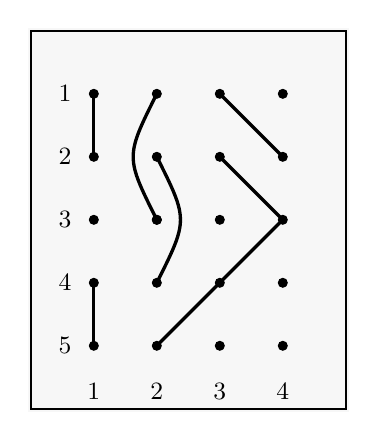
\begin{tikzpicture}[scale=0.8] 
\draw[black, thick] (0,0) rectangle (5,6);
\node[anchor=east,font=\small] at (0.8,5) {1};
\node[anchor=east,font=\small] at (0.8,4) {2};
\node[anchor=east,font=\small] at (0.8,3) {3};
\node[anchor=east,font=\small] at (0.8,2) {4};
\node[anchor=east,font=\small] at (0.8,1) {5};
\node[anchor=south,font=\small] at (1,0) {1};
\node[anchor=south,font=\small] at (2,0) {2};
\node[anchor=south,font=\small] at (3,0) {3};
\node[anchor=south,font=\small] at (4,0) {4};
\filldraw [black] (1,1) circle (2pt);
\filldraw [black] (2,1) circle (2pt);
\filldraw [black] (3,1) circle (2pt);
\filldraw [black] (4,1) circle (2pt);
\filldraw [black] (1,2) circle (2pt);
\filldraw [black] (2,2) circle (2pt);
\filldraw [black] (3,2) circle (2pt);
\filldraw [black] (4,2) circle (2pt);
\filldraw [black] (1,3) circle (2pt);
\filldraw [black] (2,3) circle (2pt);
\filldraw [black] (3,3) circle (2pt);
\filldraw [black] (4,3) circle (2pt);
\filldraw [black] (2,3) circle (2pt);
\filldraw [black] (1,4) circle (2pt);
\filldraw [black] (2,4) circle (2pt);
\filldraw [black] (3,4) circle (2pt);
\filldraw [black] (4,4) circle (2pt);
\filldraw [black] (1,5) circle (2pt);
\filldraw [black] (2,5) circle (2pt);
\filldraw [black] (3,5) circle (2pt);
\filldraw [black] (4,5) circle (2pt);
\draw[very thick] (1,5) -- (1,4); 
\draw[very thick] (3,5) -- (4,4);
\draw[very thick] (1,2) -- (1,1);
% \draw[very thick] (2,2) -- (2,4);
\draw[very thick] (2,2) .. controls (2.5,3) .. (2,4);
\draw[very thick] (2,3) .. controls (1.5,4) .. (2,5);
\draw[very thick] (2,1) -- (3,2) -- (4,3) -- (3,4);
  \begin{pgfonlayer}{background}
    \filldraw [line width=4mm,black!3]
      (0.2,0.2)  rectangle (4.8,5.8);
  \end{pgfonlayer}
\end{tikzpicture}}
\subcaptionbox{Non-crossing % non-flat
   partition.}[0.49\textwidth]{
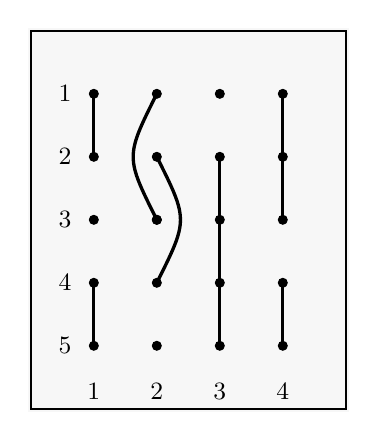
\begin{tikzpicture}[scale=0.8] 
\draw[black, thick] (0,0) rectangle (5,6);
\node[anchor=east,font=\small] at (0.8,5) {1};
\node[anchor=east,font=\small] at (0.8,4) {2};
\node[anchor=east,font=\small] at (0.8,3) {3};
\node[anchor=east,font=\small] at (0.8,2) {4};
\node[anchor=east,font=\small] at (0.8,1) {5};
\node[anchor=south,font=\small] at (1,0) {1};
\node[anchor=south,font=\small] at (2,0) {2};
\node[anchor=south,font=\small] at (3,0) {3};
\node[anchor=south,font=\small] at (4,0) {4};
\filldraw [black] (1,1) circle (2pt);
\filldraw [black] (2,1) circle (2pt);
\filldraw [black] (3,1) circle (2pt);
\filldraw [black] (4,1) circle (2pt);
\filldraw [black] (1,2) circle (2pt);
\filldraw [black] (2,2) circle (2pt);
\filldraw [black] (3,2) circle (2pt);
\filldraw [black] (4,2) circle (2pt);
\filldraw [black] (1,3) circle (2pt);
\filldraw [black] (2,3) circle (2pt);
\filldraw [black] (3,3) circle (2pt);
\filldraw [black] (4,3) circle (2pt);
\filldraw [black] (2,3) circle (2pt);
\filldraw [black] (1,4) circle (2pt);
\filldraw [black] (2,4) circle (2pt);
\filldraw [black] (3,4) circle (2pt);
\filldraw [black] (4,4) circle (2pt);
\filldraw [black] (1,5) circle (2pt);
\filldraw [black] (2,5) circle (2pt);
\filldraw [black] (3,5) circle (2pt);
\filldraw [black] (4,5) circle (2pt);
\draw[very thick] (1,5) -- (1,4); 
\draw[very thick] (4,1) -- (4,2);
\draw[very thick] (4,3) -- (4,5);
\draw[very thick] (1,2) -- (1,1);
\draw[very thick] (2,2) .. controls (2.5,3) .. (2,4);
\draw[very thick] (2,3) .. controls (1.5,4) .. (2,5);
%\draw[very thick] (2,2) -- (2,4);
\draw[very thick] (3,1) -- (3,2) -- (3,3) -- (3,4);
  \begin{pgfonlayer}{background}
    \filldraw [line width=4mm,black!3]
      (0.2,0.2)  rectangle (4.8,5.8);
\end{pgfonlayer}
\end{tikzpicture}}
\caption{Examples of partition diagrams with $n=5$ and $d=4$.}
\label{fig:diagram0-1-2}
\end{figure}
 
\vspace{-.4cm}
  
\noindent 
 The role of the partition
   $\sqcap (\alpha )$ introduced in Definition~\ref{def:parti}
   is to group each set of identical entries in a
   family of $k$-tuples into a partition block.
   Later on, it will be used to identify the
   common random variables appearing
   in repeated copies of $(X_1, \ldots , X_n)$
   for the computation of joint cumulants. 
\begin{definition}
\label{def:parti}
 Given a sequence 
 $$
 \alpha   =
\left[ 
\begin{array}{c} 
\alpha_1 
\\ 
\vdots 
\\ 
\alpha_n 
\\ 
\end{array} 
\right] 
  =
\left[ 
\begin{array}{ccc}
 \alpha_1 (1) & \cdots & \alpha_1(d)
  \\
\vdots & \ddots & \vdots 
\\
 \alpha_n (1) & \cdots & \alpha_n(d)
\end{array} 
\right] 
\in ([m_1] \times \cdots \times [m_d])^n, 
$$ 
  we let $\sqcap (\alpha )$ denote the partition 
  of $[n]\times[d]$ such that each block of $\sqcap (\alpha )$
  is made of elements $(i,\ell )$ 
  that correspond to a same value of $\alpha_i (\ell )$.
%  We identify $\sqcap (\alpha )$ to the partition diagram constructed on the blocks of $\sqcap (\alpha )$ by: 
% \begin{enumerate}[(i)]
% \item connecting the vertices corresponding to a same value in the array $(\alpha_i(l))_{(i,l) \in [j]\times [k]}$. 
% \end{enumerate}
% for each $a=(\alpha_1,\dots, \alpha_j)\in M_{j,k}$, $\sqcap (a)\in\Pi([j]\times[k])$ is given that any two elements $(i_1,\ell_1),(i_2,\ell_2)\in[j]\times[k]$ belong to the same block in $\sqcap (a)$ if and only if when $\alpha_{i_1}(\ell_1)=\alpha_{i_2}(\ell_2)$.
\end{definition}
% Intuitively, we can understand the index set $M_{j,k}$ %, the mapping $T$ and the count $C_n(\rho)$ 
% in a combinatorial way. 
% \begin{enumerate} \item There are $n$ balls with numbering in a box. \item Draw $k$ balls consecutively from the box. Put them back after noting down all their numbers. \item Repeating the previous step for $j$ times. \end{enumerate}
% We can use the following set partition diagram to visualize the mapping $T$.
% For $a=(\alpha_1,\dots,\alpha_j)\in [n]^k_{\ne}\times \cdots \times [n]^k_{\ne}$ the partition $\sqcap (a)$ can be visualized by: 
Next is an example of a sequence
$\alpha % =(\alpha_1,\dots, \alpha_j) 
\in ([m_1] \times \cdots \times [m_d])^n$
 and of the partition $\sqcap (\alpha )$ of $[n]\times [d]$ it generates. 
\begin{example}
  Taking $n=5$, $d=4$,
  $m_1=10,m_2=15,m_3=5,m_4=20$
  and
  $\alpha \in ([10] \times [15] \times [5] \times [20])^5$
  of the form
  $$
  \alpha
  =
\left[ 
\begin{array}{c} 
\alpha_1 
\\ 
\alpha_2 
\\ 
\alpha_3 
\\ 
\alpha_4 
\\ 
\alpha_5 
\\ 
\end{array} 
\right] 
  =
\left[ 
\begin{array}{cccc}
9 & 14 & 5 & 11\\
9 & 15 & 2 & 11\\
4 & 14 & 2 & 11\\
10 & 15 & 2 & 19\\
10 & 3  & 2 & 19 
\end{array} 
\right] 
,
$$ 
yields a non-crossing partition $\sqcap (\alpha )$ of
$[5]\times [4]$ given
in Figure~\ref{fig:diagram1}
 by % we further have 
  \begin{align*}
    \sqcap (\alpha )=\big\{ &\{(1,1),(2,1)\},
    \{(3,1)\},
    \{(4,1),(5,1)\},
    \{(1,2),(3,2)\},
    \{(2,2),(4,2)\},
    \\
    &
    \{(5,2)\},
    \{(1,3)\}, 
    \{(2,3),(3,3),(4,3),(5,3)\},
    \{(1,4),(2,4)(3,4)\}, 
    \{(4,4),(5,4)\}
    \big\}. 
  \end{align*}
\end{example}

\begin{figure}[H]
  \captionsetup[subfigure]{font=footnotesize}
  \centering
  \subcaptionbox{$\alpha =[\alpha_1,\dots,\alpha_5]^\top$.}[.5\textwidth]{%
  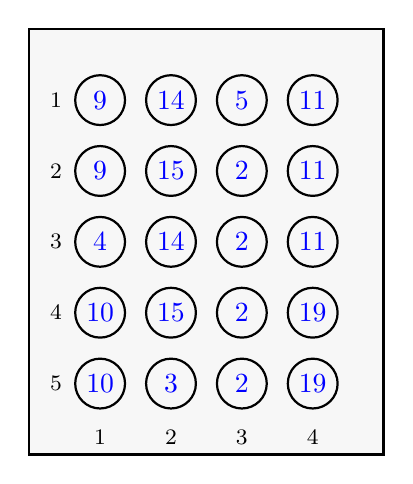
\begin{tikzpicture}[scale=0.9] 
  \draw[black, thick] (0,0) rectangle (5,6);

  \node[anchor=east,font=\footnotesize] at (0.6,5) {1};
  \node[anchor=east,font=\footnotesize] at (0.6,4) {2};
  \node[anchor=east,font=\footnotesize] at (0.6,3) {3};
  \node[anchor=east,font=\footnotesize] at (0.6,2) {4};
  \node[anchor=east,font=\footnotesize] at (0.6,1) {5};
  
  \node[anchor=south,font=\footnotesize] at (1,0) {1};
  \node[anchor=south,font=\footnotesize] at (2,0) {2};
  \node[anchor=south,font=\footnotesize] at (3,0) {3};
  \node[anchor=south,font=\footnotesize] at (4,0) {4};
  
  \foreach \i in {1,...,5}
         {
\draw[thick,black] (1,\i) circle (10pt);
\draw[thick,black] (2,\i) circle (10pt);
\draw[thick,black] (3,\i) circle (10pt);
\draw[thick,black] (4,\i) circle (10pt);
} 
\node[blue,font=\normalsize] at (1,1) {10};
\node[blue,font=\normalsize] at (1,2) {10};
\node[blue,font=\normalsize] at (1,3) {4};
\node[blue,font=\normalsize] at (1,4) {9};
\node[blue,font=\normalsize] at (1,5) {9};
\node[blue,font=\normalsize] at (2,1) {3};
\node[blue,font=\normalsize] at (2,2) {15};
\node[blue,font=\normalsize] at (2,3) {14};
\node[blue,font=\normalsize] at (2,4) {15};
\node[blue,font=\normalsize] at (2,5) {14};
\node[blue,font=\normalsize] at (3,1) {2};
\node[blue,font=\normalsize] at (3,2) {2};
\node[blue,font=\normalsize] at (3,3) {2};
\node[blue,font=\normalsize] at (3,4) {2};
\node[blue,font=\normalsize] at (3,5) {5};
\node[blue,font=\normalsize] at (4,1) {19};
\node[blue,font=\normalsize] at (4,2) {19};
\node[blue,font=\normalsize] at (4,3) {11};
\node[blue,font=\normalsize] at (4,4) {11};
\node[blue,font=\normalsize] at (4,5) {11};
  % \draw[very thick] (1,5) -- (1,4) -- (2,4) -- (3,4);
  % \draw[very thick] (2,5) -- (3,5) -- (4,5) -- (4,4);
  
  % \draw[very thick] (1,2) -- (1,1);
  % \draw[very thick] (2,3) -- (2,2);
  % \draw[very thick] (2,1) -- (3,1) -- (4,1);
  % \draw[very thick] (3,2) -- (4,3);
  
 \begin{pgfonlayer}{background}
    \filldraw [line width=4mm,black!3]
      (0.2,0.2)  rectangle (4.8,5.8);
  \end{pgfonlayer}
  \end{tikzpicture}}%
\subcaptionbox{Partition $\sqcap (\alpha )$.}[.5\textwidth]{
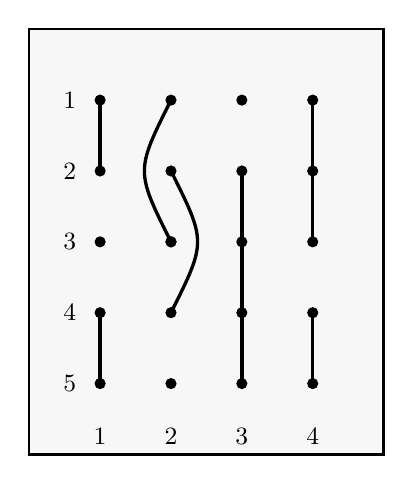
\begin{tikzpicture}[scale=0.9] 
\draw[black, thick] (0,0) rectangle (5,6);
\node[anchor=east,font=\small] at (0.8,5) {1};
\node[anchor=east,font=\small] at (0.8,4) {2};
\node[anchor=east,font=\small] at (0.8,3) {3};
\node[anchor=east,font=\small] at (0.8,2) {4};
\node[anchor=east,font=\small] at (0.8,1) {5};
\node[anchor=south,font=\small] at (1,0) {1};
\node[anchor=south,font=\small] at (2,0) {2};
\node[anchor=south,font=\small] at (3,0) {3};
\node[anchor=south,font=\small] at (4,0) {4};
\filldraw [black] (1,1) circle (2pt);
\filldraw [black] (2,1) circle (2pt);
\filldraw [black] (3,1) circle (2pt);
\filldraw [black] (4,1) circle (2pt);
\filldraw [black] (1,2) circle (2pt);
\filldraw [black] (2,2) circle (2pt);
\filldraw [black] (3,2) circle (2pt);
\filldraw [black] (4,2) circle (2pt);
\filldraw [black] (1,3) circle (2pt);
\filldraw [black] (2,3) circle (2pt);
\filldraw [black] (3,3) circle (2pt);
\filldraw [black] (4,3) circle (2pt);
\filldraw [black] (2,3) circle (2pt);
\filldraw [black] (1,4) circle (2pt);
\filldraw [black] (2,4) circle (2pt);
\filldraw [black] (3,4) circle (2pt);
\filldraw [black] (4,4) circle (2pt);
\filldraw [black] (1,5) circle (2pt);
\filldraw [black] (2,5) circle (2pt);
\filldraw [black] (3,5) circle (2pt);
\filldraw [black] (4,5) circle (2pt);
\draw[very thick] (1,5) -- (1,4); 
\draw[very thick] (4,1) -- (4,2);
\draw[very thick] (4,3) -- (4,5);
\draw[very thick] (1,2) -- (1,1);
\draw[very thick] (2,2) .. controls (2.5,3) .. (2,4);
\draw[very thick] (2,3) .. controls (1.5,4) .. (2,5);
%\draw[very thick] (2,2) -- (2,4);
\draw[very thick] (3,1) -- (3,2) -- (3,3) -- (3,4);
  \begin{pgfonlayer}{background}
    \filldraw [line width=4mm,black!3]
      (0.2,0.2)  rectangle (4.8,5.8);
\end{pgfonlayer}
\end{tikzpicture}}
  \caption{Example for the mapping $\sqcap$ with $n=5$ and $d=4$.}
  \label{fig:diagram1}
  \end{figure}
  
  \vspace{-0.4cm}

\noindent
In \cite{LiuPrivault}, a graphical diagrammatic framework was developed for representing cumulants of subgraph counts in the random-connection model and was later extended to subgraphs with fixed endpoints (see~\cite{LiuPri23b}). The $k$-hop counts studied in the present paper constitute a special case of such subgraph counts with fixed endpoints. For completeness, we adapt the diagrammatic framework to the current setting.
\begin{definition}
% \label{defgraph-1}
  {\cite{LiuPri23b}}
%  Let $G$ be a connected graph of order $r+m$ satisfying Assumption~\ref{a0}, and 
  Let $\rho=\{b_1,\dots,b_{|\rho |} \} \in \Pi([n]\times[d])$, $n \geq 1$, be 
  a partition of $[n]\times[d]$. Denote $G$ a path of order $k+1$. 
    We let $\widehat{\rho}$ denote the connected multigraph
  built on $[2]\cup([n]\times[d])$, which is constructed as follows.  
     \begin{enumerate}  
     \item For all $i\in[n]$ and $j_1,j_2\in[d]$, $j_1\ne j_2$, an edge links $(i,j_1)$ to $(i,j_2)$ iff $|j_1-j_2|=1$;
     \item For all $i\in[n]$, an edge links $(1)$ to $(i,1)$ and an edge links $(2)$ to $(i,d)$;
     \item For all $i\in[|\rho |]$, all elements in the same block $b_i$ are regarded as one vertex.
    \end{enumerate}
 In addition, we let $\rho_G$ be the graph constructed
from the multigraph $\widehat{\rho}$ % on the blocks of $\rho$
by replacing multiple edges with simple edges in $\widehat{\rho}$. 
% so that at most one edge remains between any two blocks $\rho_1,\rho_2\in\rho$. 
\end{definition}
In what follows, the blocks of any
given partition $\rho=\{b_1,\dots,b_{|\rho |} \}$
in $\Pi([n]\times[d])$ are ordered along the lexicographic order
on $[n]\times[d]$,
 by ordering the blocks according to their smallest elements.
From the above construction, the vertices of $\rho_G$ originate
from terminal nodes $[2]$ and blocks $b_1,\ldots , b_{|\rho |}$ of $\rho$.
We can further denote the vertex set of the graph $\rho_G$ as $V(\rho_G):=\left[|\rho|+2\right]$ according to the rule that the $2$ terminal nodes follows $b_1,\ldots , b_{|\rho |}$ in order.
% See also \cite{khorunzhiy} for a diagram representation used for lines and cycles in the Erd{\H o}s-R\'enyi model, and \cite{FGY23} for a graphical representation defined for the $U$-statistics of determinantal point processes.
\begin{example}
  Consider $\rho\in\Pi([3]\times[4])$ with 
  \begin{align*}
    \rho&= \big\{
    \{(1,1),(2,1),(3,1)\},
    \{(1,2)\}, \{(2,2),(3,2)\},
    \\
    &
    \quad \ \ \ \!
    \{(1,3)\}, \{(2,3)\}, \{(3,3)\},
    \{(1,4),(2,4)\}, \{((3,4)\}
    \big\}.
  \end{align*}
  Figure~\ref{fig:diagram1-2} presents the multigraph $\widehat{\rho}$ and
  its corresponding graph $\rho_G$. 
  
  \smallskip

\begin{figure}[H]
\captionsetup[subfigure]{font=footnotesize}
\centering
\subcaptionbox{Multigraph $\widehat{\rho}$ before merging edges and vertices.}[.5\textwidth]{%
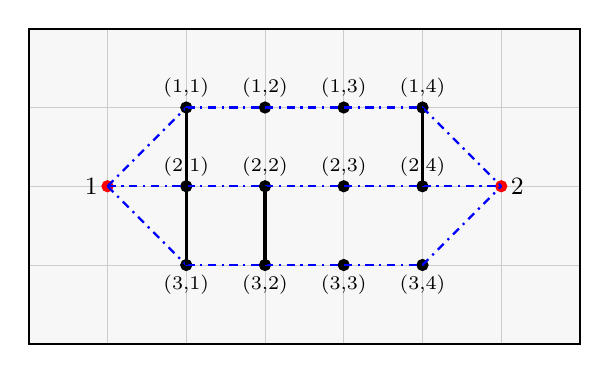
\begin{tikzpicture}% [scale=0.8] 
\draw[step=1cm, very thin, gray!40] (0,0) grid (7,4);
\draw[black, thick] (0,0) rectangle (7,4);
\filldraw [red] (1,2) circle (2pt);
\filldraw [red] (6,2) circle (2pt);
\foreach \i in {2,3}
{
\filldraw [black] (2,\i) circle (2pt);
\filldraw [black] (3,\i) circle (2pt);
\filldraw [black] (4,\i) circle (2pt);
\filldraw [black] (5,\i) circle (2pt);
\draw[thick, dash dot,blue] (2,\i) -- (3,\i);
\draw[thick, dash dot,blue] (3,\i) -- (4,\i);
% \draw[thick, dash dot,blue] (2,\i) .. controls (3,\i-0.5) .. (4,\i);
\draw[thick, dash dot,blue] (1,2) -- (2,\i);
\draw[thick, dash dot,blue] (4,\i) -- (5,\i);
}

\filldraw [black] (2,1) circle (2pt);
\filldraw [black] (3,1) circle (2pt);
\filldraw [black] (4,1) circle (2pt);
\filldraw [black] (5,1) circle (2pt);
\draw[thick, dash dot,blue] (2,1) -- (3,1);
% \draw[thick, dash dot,blue] (2,1) .. controls (3,1+0.5) .. (4,1);
\draw[thick, dash dot,blue] (3,1) -- (4,1);
\draw[thick, dash dot,blue] (1,2) -- (2,1);
\draw[thick, dash dot,blue] (4,1) -- (5,1);
\draw[thick, dash dot,blue] (5,1) -- (6,2);
\draw[thick, dash dot,blue] (5,2) -- (6,2);
\draw[thick, dash dot,blue] (5,3) -- (6,2);

\node[anchor=north,font=\scriptsize] at (2,1) {(3,1)};
\node[anchor=north,font=\scriptsize] at (3,1) {(3,2)};
\node[anchor=north,font=\scriptsize] at (4,1) {(3,3)};
\node[anchor=north,font=\scriptsize] at (5,1) {(3,4)};
\node[anchor=south,font=\scriptsize] at (2,3) {(1,1)};
\node[anchor=south,font=\scriptsize] at (3,3) {(1,2)};
\node[anchor=south,font=\scriptsize] at (4,3) {(1,3)};
\node[anchor=south,font=\scriptsize] at (5,3) {(1,4)};
\node[anchor=south,font=\scriptsize] at (2,2) {(2,1)};
\node[anchor=south,font=\scriptsize] at (3,2) {(2,2)};
\node[anchor=south,font=\scriptsize] at (4,2) {(2,3)};
\node[anchor=south,font=\scriptsize] at (5,2) {(2,4)};

% \filldraw [black] (1,2) circle (2pt);
% \node[anchor=east,font=\small] at (1,2) {$(1)$};
\node[anchor=east,font=\small] at (1,2) {$1$};
\node[anchor=west,font=\small] at (6,2) {$2$};
\draw[very thick] (3,1) -- (3,2);
\draw[very thick] (5,2) -- (5,3);
\draw[very thick] (2,3) -- (2,1);
% \draw[very thick] (4,2) -- (4,3);
  \begin{pgfonlayer}{background}
    \filldraw [line width=4mm,black!3]
      (0.2,0.2)  rectangle (6.8,3.8);
  \end{pgfonlayer}
\end{tikzpicture}}%
\subcaptionbox{Graph $\rho_G$ after merging edges. % and vertices.
}[.5\textwidth]{
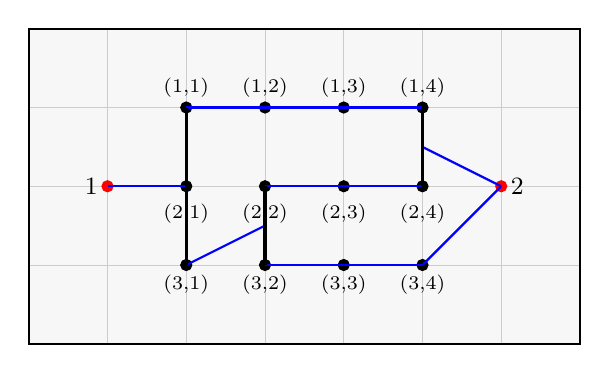
\begin{tikzpicture}% [scale=0.8] 
\draw[step=1cm, very thin, gray!40] (0,0) grid (7,4);
\draw[black, thick] (0,0) rectangle (7,4);
\filldraw [red] (1,2) circle (2pt);
\filldraw [red] (6,2) circle (2pt);
\foreach \i in {2,3}
{
\filldraw [black] (2,\i) circle (2pt);
\filldraw [black] (3,\i) circle (2pt);
\filldraw [black] (4,\i) circle (2pt);
\filldraw [black] (5,\i) circle (2pt);
}

\filldraw [black] (2,1) circle (2pt);
\filldraw [black] (3,1) circle (2pt);
\filldraw [black] (4,1) circle (2pt);
\filldraw [black] (5,1) circle (2pt);

\draw[thick, blue] (1,2) -- (2,2);
\draw[thick, blue] (2,1) -- (3,1.5);
\draw[thick, blue] (3,1) -- (4,1);
\draw[thick, blue] (4,1) -- (5,1);

\draw[thick, blue] (2,3) -- (3,3);
\draw[thick, blue] (3,3) -- (4,3);
\draw[thick, blue] (4,3) -- (5,3);
\draw[thick, blue] (5,2.5) -- (6,2);

\draw[thick, blue] (3,2) -- (4,2);
\draw[thick, blue] (4,2) -- (5,2);

\draw[thick, blue] (5,1) -- (6,2);

\node[anchor=north,font=\scriptsize] at (2,1) {(3,1)};
\node[anchor=north,font=\scriptsize] at (3,1) {(3,2)};
\node[anchor=north,font=\scriptsize] at (4,1) {(3,3)};
\node[anchor=north,font=\scriptsize] at (5,1) {(3,4)};
\node[anchor=south,font=\scriptsize] at (2,3) {(1,1)};
\node[anchor=south,font=\scriptsize] at (3,3) {(1,2)};
\node[anchor=south,font=\scriptsize] at (4,3) {(1,3)};
\node[anchor=south,font=\scriptsize] at (5,3) {(1,4)};
\node[anchor=south,font=\scriptsize] at (2,1.4) {(2,1)};
\node[anchor=south,font=\scriptsize] at (3,1.4) {(2,2)};
\node[anchor=south,font=\scriptsize] at (4,1.4) {(2,3)};
\node[anchor=south,font=\scriptsize] at (5,1.4) {(2,4)};

\node[anchor=east,font=\small] at (1,2) {$1$};
\node[anchor=west,font=\small] at (6,2) {$2$};
\draw[very thick] (3,1) -- (3,2);
\draw[very thick] (5,2) -- (5,3);
\draw[very thick] (2,3) -- (2,1);

\begin{pgfonlayer}{background}
    \filldraw [line width=4mm,black!3]
      (0.2,0.2)  rectangle (6.8,3.8);
  \end{pgfonlayer}
\end{tikzpicture}}%
\caption{
  Example of graph $\rho_G$
 with $n=3$, and $d=4$.}
\label{fig:diagram1-2}
\end{figure}

\vspace{-0.8cm}

\end{example}
% \subsubsection*{Moments and cumulants of subgraph counts} 

\noindent 
 Lemma~\ref{fkla12} is analog to
 Lemma~2.8 in \cite{LiuPrivault}
 or Proposition 6.1 in \cite{schulte-thaele}
 for non-crossing partitions. 
       \begin{lemma}
         \label{fkla12}
          \noindent
        $a)$ The cardinality of the set \ ${\rm CNC}([n]\times [d])$
       of connected non-crossing partitions of $[n]\times[d]$ satisfies 
       \begin{equation}
         \label{coeff-0}
        |{\rm CNC}([n]\times [d])| \leq n!^d, 
        \qquad n,d \geq 1. 
      \end{equation}
      \noindent
      $b)$ \textcolor{red}{Given $n\ge1$ and $d\ge2$, we denote by 
      $$
      \mathcal{M}(n,d):=\{\rho\in{\rm CNC}([n]\times [d]): |\rho|=1+(d-1)n\}
      $$
      the set of maximal connected non-crossing partition of $[n]\times[d]$.
}
       The cardinality of the set 
      $\mathcal{M}(n,d)$
       of maximal connected non-crossing partitions of $[n]\times[d]$
       satisfies
                   $|\mathcal{M}(1,d)|=1$ and              
      \begin{equation}
        \label{coeff-10}
        |\mathcal{M}(n,d)|=d, \qquad n\geq 2, \ d\geq 1. 
      \end{equation}
      \end{lemma} 
\begin{Proof}
\noindent
 $a)$ We clearly have $|{\rm NC} (1,d) | =1$ for all $d\geq 1$. 
% As a consequence of Lemma~\ref{restrict-partition},
Any % connected
 non-crossing partition $\rho \in {\rm NC}(n+1,d)$ can be
 obtained from a % connected
  non-crossing partition in ${\rm NC}(n,d)$ in at most
 $(n+1)^d$ ways, by connecting each of the $d$ new points
 in at most $n+1$ possible ways (including non-connection). 
 This yields the induction inequality 
 $$
 |{\rm NC} (n+1,d) | \leq (n+1)^d | {\rm NC} (n,d) |,
 $$
 from which we conclude that \eqref{coeff-0} holds. 
 
 \medskip 

 \noindent
 $b)$ 
 We clearly have $|\mathcal{M}(1,d)|=1$ and
 $|\mathcal{M}(2,d)|=d$ for all $d\geq 1$.
 Next, each maximal connected non-crossing partition 
 $\rho\in \mathcal{M}(n+1,d)$ is obtained in
 a unique way from any partition in $\mathcal{M}(n,d)$, $n\geq 1$,
 which yields \eqref{coeff-10}. 
\end{Proof} 
\section{Joint moments of $k$-hop counts} 
\label{sec4}
Proposition~\ref{p1} provides a combinatorial expression for the joint 
 moments of $(\sigma_k(t_1),\ldots ,\sigma_k(t_n))$ for any 
 $t_1 , \ldots , t_n \in [(k-1)r,kr]$, 
 using sums over non-crossing partitions of $[n]\times [d]$. % \{1,\ldots , n\}$. 
% Letting $\rho_{K_k}$ denote the contraction graph of the complete graph $K_k$ on $k$ vertices,
 \textcolor{red}{
  Given $j\ge1$ and $f^{(i)}:[0,r]^d \to\real$, $i=1,\dots,j$,
       measurable functions, we let 
       \begin{equation}
         \nonumber % \label{def:tensorproduct-1}
       \left(\bigotimes_{i=1}^jf^{(i)} \right)(x_{1,1},\ldots,x_{1,d},\ldots,
       x_{j,1},\ldots , x_{j,d}):=\prod_{i=1}^jf^{(i)} (x_{i,1},\dots,x_{i,d}), 
      % \qquad x_1,\dots,x_N\in \R^d.
\end{equation}
  and for $\rho\in \Pi([j] \times [d] )$ we denote by 
        $$
        \left(
	\bigotimes_{i=1}^jf^{(i)} \right)_{\! \! \! \rho} \ \! : \ \! [0,r]^{|\rho|}\to\real
        $$
        the function obtained by equating any two variables
        whose indexes belong to a same block of $\rho$.
}
% For any set partition
% $\rho =\{b_1,\dots,b_{|\rho |}\}\in\Pi([n]\times[d])$
% and bounded measurable function
% $f:[0,r]^d \to\real $, consider the function 
%$$
%\left(\bigotimes_{i=1}^n f
%\right)_{\! \! \! \rho }
% \ \! : \ \! [0,r]^{|\rho |} \to\real
%$$
% defined as 
%\begin{eqnarray*}
%\left(\bigotimes_{i=1}^n f
%\right)_{\! \! \! \rho }
%( x_1, \ldots , x_{|\rho |} ) :=\prod_{i=1}^n 
%f\big(x^{(i)}_1,\dots,x^{(i)}_d \big),
%\end{eqnarray*}
% where $x^{(i)}_\ell:=x_n$ if $(i,\ell)\in b_n$, 
% $n = 1 , \ldots , |\rho |$. 
 In Proposition~\ref{p1}, we 
 provide an identity for the joint moments of $k$-hop counts. 
\begin{prop}
\label{p1}
  Let $d\geq 1$. 
  For any $n \geq 1$ and $t_1,\ldots , t_n \in [(k-1)r,kr]$,
   \textcolor{red}{the joint moment of $\sigma_k(t_i)$ is given by}
\begin{align} 
\label{djkls12}
& \E  [ \sigma_k(t_1) \cdots  \sigma_k(t_n)  ] 
\\
\nonumber
& = \sum_{
 \rho\in {\rm NC} ([n]\times[d])
}
p^{e(\rho_G)}
\left(
 \prod_{i=1}^d \frac{m_i!}{(m_i - |\rho_i| )!}
 \right)
 \int_{
    [0,r]^{|\rho|}
  }\left(\bigotimes_{i=1}^n
 u_{t_i} \right)_{\! \! \! \rho}
 ( x_1, \ldots , x_{|\rho|} ) 
 \textcolor{red}{\prod_{j=1}^{|\rho|} \mu_{\bar{b}_j} ( \mathrm{d} x_j ). }
\end{align} 
 \textcolor{red}{Here, $\rho=\{b_1,\dots,b_{|\rho |} \}\in {\rm NC} ([n]\times[d])$
 is written as 
$\rho=\bigcup_{i=1}^d\rho_i$, see \eqref{fjklds143}.
 Moreover, %$u_t : [0,r]^d \mapsto \{0,1\}$ is the indicator function of $d$ variables given by 
\begin{equation}
\label{jklf12} 
 u_t (x_1 , \ldots , x_d)
 := {\bf1}_{\{x_1 \leq \cdots \leq x_d \leq kr-t \}},
 \quad x_1,\ldots , x_d \in [0,r], 
\end{equation} 
and $\bar{b}_i$ denotes the unique $k\in \{1,\ldots ,d\}$ such that $b_i\in\rho_k$.}
\end{prop}
\begin{Proof}
 For any $t_1,\ldots , t_n \in [0,r]$,
 as in the proof of Theorem~3.2 in \cite{LiuPrivault25}, 
 we have 
\begin{align*} 
\nonumber 
& \E  [ \sigma_k(t_1) \cdots  \sigma_k(t_n)  ] 
\\
 & = \sum_{\alpha_i\in [m_1]\times \cdots \times [m_d]
  \atop
  1 \leq i \leq n
  }
  \E\left[
 \prod_{i=1}^n
 \Big(
  Y^{(0)}_{\alpha_i(1)}Y^{(1)}_{\alpha_i(1),\alpha_i(2)}\cdots Y^{(d-1)}_{\alpha_i(d-1),\alpha_i(d)} Y^{(d)}_{\alpha_i(d)}
 u_{t_i} \big(U^{(1)}_{\alpha_i(1)} , \ldots , U^{(d)}_{\alpha_i(d)}\big) \Big) 
 \right]
 \\
 & = 
     \sum_{\substack{\rho\in\Pi([n]\times [d])\\\rho\wedge\pi=\widehat{0}}}
        \sum_{\alpha_i\in [m_1]\times \cdots \times [m_d]
  \atop
1\leq i \leq n}
        \hskip-0.8cm
                {\bf 1}_{\{ \sqcap (\alpha ) = \rho \}}                 
   \E\left[
 \prod_{i=1}^n
 \Big(
  Y^{(0)}_{\alpha_i(1)}Y^{(1)}_{\alpha_i(1),\alpha_i(2)}\cdots Y^{(d-1)}_{\alpha_i(d-1),\alpha_i(d)} Y^{(d)}_{\alpha_i(d)}
 u_{t_i} \big(U^{(1)}_{\alpha_i(1)} , \ldots , U^{(d)}_{\alpha_i(d)}\big) \Big) 
 \right]
 \\
 & = 
 \sum_{\textcolor{red}{\rho\in {\rm NC}([n]\times [d])}}
        \sum_{\alpha_i\in [m_1]\times \cdots \times [m_d]
  \atop
1\leq i \leq n}
        \hskip-0.8cm
                {\bf 1}_{\{ \sqcap (\alpha ) = \rho \}}                 
    \E\left[
 \prod_{i=1}^n
 \Big(
  Y^{(0)}_{\alpha_i(1)}Y^{(1)}_{\alpha_i(1),\alpha_i(2)}\cdots Y^{(d-1)}_{\alpha_i(d-1),\alpha_i(d)} Y^{(d)}_{\alpha_i(d)}
 u_{t_i} \big(U^{(1)}_{\alpha_i(1)} , \ldots , U^{(d)}_{\alpha_i(d)}\big) \Big) 
 \right]
       \\
&=\sum_{\textcolor{red}{\rho\in {\rm NC}([n]\times [d])}}
 p^{e(\rho_G)}
 \sum_{\textcolor{red}{\alpha\in
	 ([m_1] \times \cdots \times [m_d])^n}
    \atop \sqcap (\alpha ) = \rho }
    \int_{[0,r]^{|\rho|}} \left(\bigotimes_{i=1}^n u_{t_i} \right)_{\! \! \! \rho}
      ( x_1, \ldots , x_{|\rho|} ) 
 \mu_{\bar{\rho}_1} ( d x_1 ) 
 \cdots
 \mu_{\bar{\rho}_{|\rho|}} ( d x_{|\rho|} ) 
% (\mathbf{x})\mu^{\otimes |\rho|} ( \mathrm{d}\mathbf{x} )
\\
&=\sum_{\textcolor{red}{\rho\in {\rm NC}([n]\times [d])}}
C_{m_1,\ldots , m_d} (\rho)
 p^{e(\rho_G)}
\int_{
   [0,r]^{|\rho|}}\left(\bigotimes_{i=1}^n u_{t_i} \right)_{\! \! \! \rho}
  ( x_1, \ldots , x_{|\rho|} ) 
 \mu_{\bar{\rho}_1} ( d x_1 ) 
 \cdots
 \mu_{\bar{\rho}_{|\rho|}} ( d x_{|\rho|} ) 
% (\mathbf{x})\mu^{\otimes |\rho|} ( \mathrm{d}\mathbf{x} )
,
\end{align*}
where
$$
 C_{m_1,\ldots , m_d}(\rho)
 = \prod_{i=1}^d \frac{m_i!}{(m_i - |\rho_i| )!} 
$$ 
 represents the count of the 
 $\alpha  = [\alpha_1,\ldots , \alpha_n]^\top \in
 ([m_1] \times \cdots \times [m_d])^n$
 such that $\sqcap (\alpha )=\rho$,
 $n,k\geq 1$, with $\rho$ non-crossing. 
\end{Proof}
 In particular, in the case of $2$-hops with $d=1$,
 we have 
$$ 
 \E  [ \sigma_2(t_1) \cdots  \sigma_2(t_n)  ] 
  = \sum_{\rho\in \Pi ([n] )} 
 \frac{p^{2 | \rho |}m_1!}{(m_1 - |\rho| )!}
 \int_{
    [0,r]^{|\rho|}
  }\left(\bigotimes_{i=1}^n
 u_{t_i} \right)_{\! \! \! \rho}
 ( x_1, \ldots , x_{|\rho|} ) 
 \mu_1 ( d x_1 ) 
 \cdots
 \mu_1 ( d x_{|\rho|} ) 
% \mu^{\otimes |\rho|} ( \mathrm{d}\mathbf{x} )
. 
$$ 
If in addition $\mu_1$ is the uniform measure on $[0,r]$,
then 
$\sigma_2(t)$ has a binomial distribution with parameters $m_1$
and
\begin{equation}
  \label{d=1}
p^2\frac{2r-t}{r}, \qquad  t\in [r,2r]. 
\end{equation}
\subsubsection*{First moment}
When $n=1$, there is only one non-crossing partition
$\rho \in \Pi ( [1]\times [d])$, which is given as 
$\rho = \{ \{(1,1)\}, \ldots , \{(1,d) \}\}$, and
can be represented as in Figure~\ref{f2-1} for $d=8$. 

% \vskip-0.2cm

\begin{figure}[H]
\centering 
  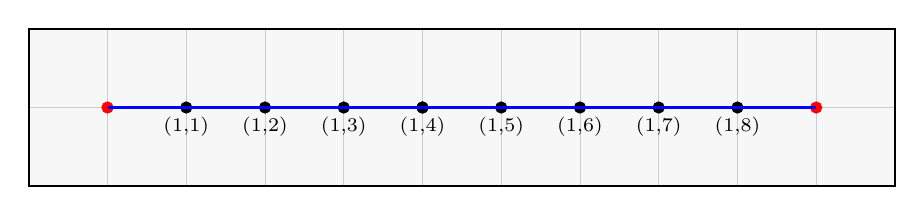
\begin{tikzpicture}% [scale=0.8] 
\draw[step=1cm, very thin, gray!40] (0,0) grid (11,2);
\draw[black, thick] (0,0) rectangle (11,2);
\filldraw [red] (1,1) circle (2pt);
\filldraw [red] (10,1) circle (2pt);

\filldraw [black] (2,1) circle (2pt);
\filldraw [black] (3,1) circle (2pt);
\filldraw [black] (4,1) circle (2pt);
\filldraw [black] (5,1) circle (2pt);
\filldraw [black] (5,1) circle (2pt);
\filldraw [black] (6,1) circle (2pt);
\filldraw [black] (7,1) circle (2pt);
\filldraw [black] (8,1) circle (2pt);
\filldraw [black] (9,1) circle (2pt);
\draw[thick, blue] (1,1) -- (2,1);
\draw[thick, blue] (1,1) -- (2,1);
\draw[thick, blue] (2,1) -- (3,1);
\draw[thick, blue] (3,1) -- (4,1);
\draw[thick, blue] (4,1) -- (5,1);
\draw[thick, blue] (5,1) -- (6,1);
\draw[thick, blue] (6,1) -- (7,1);
\draw[thick, blue] (7,1) -- (8,1);
\draw[thick, blue] (8,1) -- (9,1);
\draw[thick, blue] (9,1) -- (10,1);

\node[anchor=north,font=\scriptsize] at (2,1) {(1,1)};
\node[anchor=north,font=\scriptsize] at (3,1) {(1,2)};
\node[anchor=north,font=\scriptsize] at (4,1) {(1,3)};
\node[anchor=north,font=\scriptsize] at (5,1) {(1,4)};
\node[anchor=north,font=\scriptsize] at (6,1) {(1,5)};
\node[anchor=north,font=\scriptsize] at (7,1) {(1,6)};
\node[anchor=north,font=\scriptsize] at (8,1) {(1,7)};
\node[anchor=north,font=\scriptsize] at (9,1) {(1,8)};

% \draw[very thick] (2,1) -- (2,2);
% \draw[very thick] (3,1) -- (3,2);
% \draw[very thick] (4,1) -- (4,2);
% \draw[very thick] (5,1) -- (5,2);
% \draw[very thick] (6,1) -- (6,2);
% \draw[very thick] (7,1) -- (7,2);
% \draw[very thick] (7,1) -- (7,2);
% \draw[very thick] (8,1) -- (8,2);
% \draw[very thick] (9,1) -- (9,2);
\begin{pgfonlayer}{background}
    \filldraw [line width=4mm,black!3]
      (0.2,0.2)  rectangle (10.8,1.8);
  \end{pgfonlayer}
\end{tikzpicture}
%\vskip-0.2cm
 \caption{
 Single non-crossing partition
of $[1] \times [d]$ with $d=8$.} 
\label{f2-1}
\end{figure}

\vskip-0.4cm

\noindent
 Here, we have
 $C_{m_1,\ldots , m_d}(\rho) = m_1\cdots m_d$,
 and 
 the first moment of the count $\sigma_k(t)$ of $k$-hop paths is
 given by
\begin{align} 
\nonumber
 \E [ \sigma_k (t) ]
 & = 
 \E\left[
 \sum_{\beta \in [m_1] \times \cdots \times [m_d]}
 u_t \big(U^{(1)}_{\beta (1)} , \ldots , U^{(d)}_{\beta (d)}\big) 
 \right]
\\
\nonumber
 & = 
 \sum_{\beta \in [m_1] \times \cdots \times [m_d]}
 \E\big[
 u_t \big(U^{(1)}_{\beta (1)} , \ldots , U^{(d)}_{\beta (d)}\big) 
 \big]
\\
\nonumber
 & = 
 p^{d+1}
 m_1\cdots m_d
 \int_0^{kr-t} \int_0^{x_d} \cdots \int_0^{x_2} \mu_1(dx_1)\cdots \mu_d(dx_d). 
\end{align}
If $\mu_i$ is the uniform measure on $[0,r]$ for all
$i=1,\ldots , d$, then we have 
\begin{align} 
\nonumber
 \E [ \sigma_k (t) ]
& = 
 \frac{p^{d+1}}{r^d}
 m_1\cdots m_d 
 \int_0^{kr-t} \int_0^{x_d} \cdots \int_0^{x_2} dx_1\cdots dx_d
% {\bf1}_{\{i_1<\cdots < i_d\}} \prod_{p=1}^d {\bf 1}_{\{m_1+\cdots +m_{p-1} < i_p \leq m_1+\cdots + m_p\}}
\\
\label{fjkdls-0}
& = 
p^{d+1} m_1\cdots m_d\frac{((kr-t) / r)^d}{d!}. 
\end{align} 
 When
$$
m_1 = \cdots = m_d = 1, 
$$
 we have 
$$ 
  \E  [ \sigma_k(t) ]
 = 
  p \frac{(p(kr-t))^d}{r^dd!}, 
$$ 
 and 
$\sigma_k(t)$ is a Bernoulli random variable with parameter
$$
 \P\big(U_1^{(1)} \leq \cdots \leq U^{(d)}_1 \leq kr-t \big) =
 p \frac{(p ( kr-t) )^d}{r^dd!}. 
$$ 
\subsubsection*{Second moment}
\noindent
 When $n=2$, the count of blocks
of non-crossing partitions of $[2] \times [d]$
ranges from $d$ to $2d$, each block has size either one or two,
as in Figure~\ref{f3-1-1} for $d=8$. 

% \vskip-0.2cm

\begin{figure}[H]
\centering 
  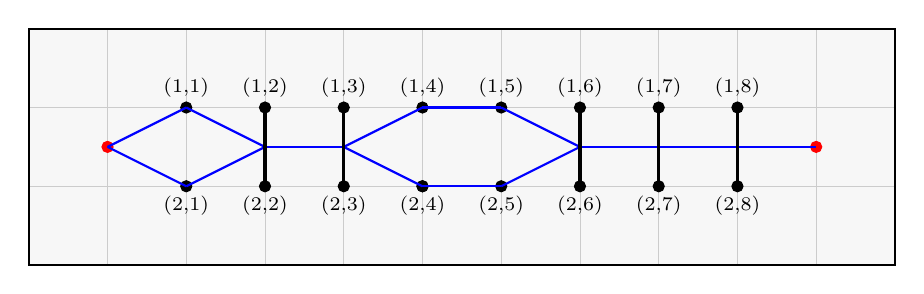
\begin{tikzpicture}% [scale=0.8] 
\draw[step=1cm, very thin, gray!40] (0,0) grid (11,3);
\draw[black, thick] (0,0) rectangle (11,3);
\filldraw [red] (1,1.5) circle (2pt);
\filldraw [red] (10,1.5) circle (2pt);
\foreach \i in {2}
{
\filldraw [black] (2,\i) circle (2pt);
\filldraw [black] (3,\i) circle (2pt);
\filldraw [black] (4,\i) circle (2pt);
\filldraw [black] (5,\i) circle (2pt);
\filldraw [black] (6,\i) circle (2pt);
\filldraw [black] (7,\i) circle (2pt);
\filldraw [black] (8,\i) circle (2pt);
\filldraw [black] (9,\i) circle (2pt);
}

\filldraw [black] (2,1) circle (2pt);
\filldraw [black] (3,1) circle (2pt);
\filldraw [black] (4,1) circle (2pt);
\filldraw [black] (5,1) circle (2pt);
\filldraw [black] (5,1) circle (2pt);
\filldraw [black] (6,1) circle (2pt);
\filldraw [black] (7,1) circle (2pt);
\filldraw [black] (8,1) circle (2pt);
\filldraw [black] (9,1) circle (2pt);
\draw[thick, blue] (1,1.5) -- (2,1);
\draw[thick, blue] (1,1.5) -- (2,2);
\draw[thick, blue] (2,2) -- (3,1.5);
\draw[thick, blue] (2,1) -- (3,1.5);
\draw[thick, blue] (3,1.5) -- (4,1.5);
\draw[thick, blue] (4,1.5) -- (5,1);
\draw[thick, blue] (4,1.5) -- (5,2);
\draw[thick, blue] (5,2) -- (6,2);
\draw[thick, blue] (5,1) -- (6,1);
\draw[thick, blue] (6,2) -- (7,1.5);
\draw[thick, blue] (6,1) -- (7,1.5);
\draw[thick, blue] (7,1.5) -- (8,1.5);
\draw[thick, blue] (8,1.5) -- (9,1.5);
\draw[thick, blue] (9,1.5) -- (10,1.5);

\node[anchor=north,font=\scriptsize] at (2,1) {(2,1)};
\node[anchor=north,font=\scriptsize] at (3,1) {(2,2)};
\node[anchor=north,font=\scriptsize] at (4,1) {(2,3)};
\node[anchor=north,font=\scriptsize] at (5,1) {(2,4)};
\node[anchor=north,font=\scriptsize] at (6,1) {(2,5)};
\node[anchor=north,font=\scriptsize] at (7,1) {(2,6)};
\node[anchor=north,font=\scriptsize] at (8,1) {(2,7)};
\node[anchor=north,font=\scriptsize] at (9,1) {(2,8)};
\node[anchor=south,font=\scriptsize] at (2,2) {(1,1)};
\node[anchor=south,font=\scriptsize] at (3,2) {(1,2)};
\node[anchor=south,font=\scriptsize] at (4,2) {(1,3)};
\node[anchor=south,font=\scriptsize] at (5,2) {(1,4)};
\node[anchor=south,font=\scriptsize] at (6,2) {(1,5)};
\node[anchor=south,font=\scriptsize] at (7,2) {(1,6)};
\node[anchor=south,font=\scriptsize] at (8,2) {(1,7)};
\node[anchor=south,font=\scriptsize] at (9,2) {(1,8)};

% \node[anchor=east,font=\small] at (1,2) {$1$};
% \node[anchor=west,font=\small] at (6,2) {$2$};
\draw[very thick] (3,1) -- (3,2);
\draw[very thick] (4,1) -- (4,2);
\draw[very thick] (7,1) -- (7,2);
\draw[very thick] (7,1) -- (7,2);
\draw[very thick] (8,1) -- (8,2);
\draw[very thick] (9,1) -- (9,2);
\begin{pgfonlayer}{background}
    \filldraw [line width=4mm,black!3]
      (0.2,0.2)  rectangle (10.8,2.8);
  \end{pgfonlayer}
\end{tikzpicture}
%\vskip-0.2cm
\caption{
 Example of a non-crossing partition
of $2 \times d$ with $d=8$.} 
\label{f3-1-1}
\end{figure}

\vspace{-0.4cm}

\begin{corollary} 
% \label{p1}
  Let $d\geq 1$ and 
  $t_1,t_2 \in [(k-1)r,kr]$. We have 
\begin{align} 
\nonumber % \label{djkls12}
& \E  [ \sigma_k(t_1) \sigma_k(t_2)  ] 
\\
\nonumber
& = \sum_{
 \rho\in {\rm NC} ([2]\times[d])
}
p^{e(\rho_G)}
\left(
 \prod_{i=1}^d \frac{m_i!}{(m_i - |\rho_i| )!}
 \right)
 \int_{
    [0,r]^{|\rho|}
 }\left(
 u_{t_1}
 \otimes
 u_{t_2}
 \right)_{\rho}
 ( x_1, \ldots , x_{|\rho|} ) 
 \mu_{\bar{\rho}_1} ( d x_1 ) 
 \cdots
 \mu_{\bar{\rho}_{|\rho|}} ( d x_{|\rho|} ) 
% \mu^{\otimes |\rho|} ( \mathrm{d}\mathbf{x} )
, 
\end{align} 
where
% $$ c(\rho ) : = |b_1|+|b_d|+\sum_{i=1}^{d-1} \min ( |b_i|,|b_{i+1}|), $$ and 
 $\bar{\rho}_i$ denotes the index $j\in \{1,\ldots , d \}$ of the unique
 vertical block
 $\eta_j = ((1,j),(2,j))$ containing $b_i$, $i=1,\ldots , |\rho|$. 
\end{corollary} 
\noindent
 In particular, in the case of $2$-hops with $d=1$, we have 
\begin{align} 
\nonumber % \label{fjkdls}
 \E  [ \sigma_2(t)^2 ]
 = 
  p^4 m_1(m_1-1)
  \left(\frac{kr-t}{r} \right)^{2}
  +
  p^2 m_1
 \frac{kr-t}{r} 
, 
\end{align} 
\noindent
 and % In particular, in the case of $2$-hops with $d=1$, we have 
\begin{align*} 
\nonumber % \label{fjkdls}
\Var [ \sigma_2(t) ]
 &  = 
% p^4 m_1(m_1-1) \left(\frac{\tau}{r}\right)^{2} + p^2 m_1 \frac{\tau}{r} - p^4m_1^2 \left(\frac{\tau}{r}\right)^2
% \\ & = p^2 m_1 \frac{\tau}{r} - p^4 m_1 \left(\frac{\tau}{r} \right)^{2}
% \\ & = 
   m_1p^2
   \frac{kr-t}{r} 
    \left( 1  -
  p^2 \frac{kr-t}{r} \right)
  . 
\end{align*} 
\noindent 
 In Proposition~\ref{djklfs2}, we compute the 
 second moment of the count $\sigma_k(t)$ of $k$-hop paths.  
% Alternatively, this result can be proved as a consequence of Corollary~\ref{c1} and the It\^o isometry for multiple Poisson stochastic integrals. 
 Higher cumulants and moments of $\sigma_k(t)$ may also 
 be computed by this method, using % Corollary~\ref{c1} above and
 Corollary~7.4.1 of \cite{peccatitaqqu}. 
\begin{prop} 
\label{djklfs2}
Let $d\geq 1$ and $t\in [(k-1)r,kr]$,
assume that $p=1$ and that $\mu_i$ is the uniform measure on $[0,r]$,
 $i=1,\ldots , d$.
 The second moment of the count $\sigma_k(t)$ of $k$-hop paths is given by
\begin{align} 
\nonumber % \label{fjkdls}
  & \E  [ \sigma_k(t)^2 ]
  \\
  \nonumber
  & =
  m_1(m_1-1)\cdots m_d(m_d-1)
  \sum_{l=0}^d
  \frac{((kr-t) / r)^{2d-l}}{(2d-l)!}
  \sum_{
    j_0 + \cdots + j_l = d-l \atop j_0,\ldots , j_l\geq 0}
 \prod_{q=1}^l 
 \frac{1}{m_{j_0+\cdots + j_{q-1} + q}-1} 
  \prod_{{q'}=0}^l
       {2j_{q'} \choose j_{q'}}. 
% \\ \nonumber & = m_1(m_1-1)\cdots m_d(m_d-1)\frac{(p\tau /r)^{2d}}{d!^2} \\ \nonumber & \quad + \sum_{l=1}^d \frac{(p\tau)^{2d-l}}{r^{2d-l}} \frac{m_1(m_1-1)\cdots m_d(m_d-1)}{(2d-l)!} \sum_{ j_0 + \cdots + j_l = d-l \atop j_0,\ldots , j_l\geq 0} \prod_{q=1}^l \frac{1}{m_{j_0+\cdots + j_{q-1} + q}-1} \prod_{p=0}^l {2j_p \choose j_p}. 
\end{align} 
\end{prop} 
\begin{Proof} 
\noindent 
Given $\rho \in {\rm NC}([2]\times[d])$,
we denote by $l$ the number of blocks of $\rho$ of
size two, and assume that they are indexed by
$i_1, \ldots , i_l$. We have 
\begin{align*} 
  &
 \int_{
    [0,r]^{|\rho|}
 }\left(
 u_{t_1}
 \otimes
 u_{t_2}
 \right)_{ \rho}
 ( x_1, \ldots , x_{|\rho|} ) 
 \mu_{\bar{\rho}_1} ( d x_1 ) 
 \cdots
 \mu_{\bar{\rho}_{|\rho|}} ( d x_{|\rho|} ) 
  \\
  & \quad
   = 
 \frac{1}{r^{2d-l}}
  \int_0^{kr-t}
\int_0^{z_{i_l}}
\cdots
\int_0^{z_{i_2}}
\prod_{j=0}^l
\frac{ (z_{i_{j+1}}-z_{i_j})^{2(i_{j+1}-i_j-1)} }{((i_{j+1}-i_j-1)!)^2}
dz_{i_1}\cdots dz_{i_l}
\\
\nonumber
& 
 \quad =
\frac{((kr-t) / r)^{2d-l}}{((i_1-1)!)^2}
    \prod_{j=1}^l
\int_0^1
\frac{ (1-y)^{2(i_{j+1}-i_j-1)}
  y^{2i_j-j-1}
}{((i_{j+1}-i_j-1)!)^2}
dy
\\
\nonumber
& 
\quad =
\frac{((kr-t) / r)^{2d-l}}{((i_1-1)!)^2}
\prod_{j=1}^l
\frac{B(2i_j-j,
2(i_{j+1}-i_j)-1)
  }{((i_{j+1}-i_j-1)!)^2}
\\
\nonumber
& 
\quad =
\frac{((kr-t) / r)^{2d-l}}{((i_1-1)!)^2}
  \prod_{j=1}^l
\frac{
(2i_j-j-1)!
(2(i_{j+1}-i_j-1))!}
     {
       (2i_{j+1}-j-2)!
     ((i_{j+1}-i_j-1)!)^2}
\\
\nonumber
& 
\quad =
\frac{((kr-t) /r)^{2d-l}}{(2d-l)!}
\prod_{j=0}^l
\frac{
(2(i_{j+1}-i_j-1))!}
     {
     ((i_{j+1}-i_j-1)!)^2}
     ,
 \end{align*} 
where we take $z_0=0$ and $z_k=kr-t$,
 $$
 B(x,y) = \int_0^1 t^{x-1}(1-t)^{y-1} dt,
 \qquad  x, y>0,
$$
 is the beta function, and
 $2^{-(i_{j+1}-i_j-1)}(2(i_{j+1}-i_j-1))! / (i_{j+1}-i_j-1)!$
 is the number of pair-partitions of $2(i_{j+1}-i_j-1)$. 
 Hence, since
$$
C_{m_1,\ldots , m_d} (\rho) = \frac{m_1(m_1-1)\cdots m_d (m_d-1)}{(m_{k_1}-1) \cdots (m_{k_l}-1)}, 
$$
 by Proposition~\ref{p1} we have 
\begin{align*} 
& \E  [ \sigma_k(t)^2 ]
% = \sum_{l=0}^d \sum_{\alpha_1(1) \in [m_1], \ldots , \alpha_1(d)\in [m_d] \atop \{i_1,\ldots , i_l \} \subset \{ \alpha_1(1), \ldots , \alpha_1(d) \} } \frac{(p \tau /r)^{2d-l}}{(2d-l)!} \prod_{j=0}^l \frac{ (2(i_{j+1}-i_j-1))!} { ((i_{j+1}-i_j-1)!)^2}
\\
 & =  
 m_1(m_1-1)\cdots m_d(m_d-1)
  \sum_{l=0}^d
  \frac{(kr-t)^{2d-l}}{r^{2d-l}(2d-l)!}
  \sum_{
    j_0 + \cdots + j_l = d-l \atop j_0,\ldots , j_l\geq 0}
 \prod_{q=1}^l 
 \frac{1}{m_{j_0+\cdots + j_{q-1} + q}-1} 
  \prod_{{q'}=0}^l
       {2j_{q'} \choose j_{q'}}
 . 
\end{align*}
\end{Proof}
 \noindent 
  From Proposition~\ref{djklfs2}, the
 variance of the count $\sigma_k(t)$ of $k$-hop paths is given by 
\begin{align} 
\nonumber % \label{dfjkvar}
  \Var [ \sigma_k(t) ]
 & =
  - \frac{m_1^2\cdots m_d^2}{d!^2}
  \\
  \nonumber 
   & \quad + 
  \sum_{l=0}^d
  \frac{m_1(m_1-1)\cdots m_d(m_d-1)}{(2d-l)!}
  \sum_{
    j_0 + \cdots + j_l = d-l \atop j_0,\ldots , j_l\geq 0}
 \prod_{q=1}^l 
 \frac{1}{m_{j_0+\cdots + j_{q-1} + q}-1} 
  \prod_{{q'}=0}^l
       {2j_{q'} \choose j_{q'}}
       \\
       \nonumber
       & =
       \frac{m_1(m_1-1)\cdots m_d(m_d-1)}{d!^2} 
  - \frac{m_1^2\cdots m_d^2}{d!^2}
  \\
  \nonumber 
   & \quad + 
  \sum_{l=1}^d
  \frac{m_1(m_1-1)\cdots m_d(m_d-1)}{(2d-l)!}
  \sum_{
    j_0 + \cdots + j_l = d-l \atop j_0,\ldots , j_l\geq 0}
 \prod_{q=1}^l 
 \frac{1}{m_{j_0+\cdots + j_{q-1} + q}-1} 
  \prod_{{q'}=0}^l
       {2j_{q'} \choose j_{q'}}.
\end{align} 
 In case the point counts are equal to $m$ on all cells,  
% on all lenses,
 we obtain the following variance result.
\begin{corollary} 
\label{djklfs2-2}
Let $d\geq 1$ and assume that $p=1$, that $\mu_i$ is the uniform measure on $[0,r]$, 
$i=1,\ldots , d$, and that $m_1 = \cdots = m_d = m$. 
% $\lambda_i=\lambda$, and let
% $a_{k,i} = a_k$, $i=1,\ldots , k-1$. 
 Then, for $t \in [(k-1)r,kr]$, the variance 
 of the $k$-hop path count $\sigma_k (t)$ is given by
\begin{align} 
\nonumber % \label{dfjkvar} 
  \Var_m [ \sigma_k(t) ]
 & =
  m^d( (m-1)^d - m^d ) 
  \frac{((kr-t)/r)^{2d}}{d!^2}
  \\
  \nonumber
  & \quad + 
  \sum_{l=1}^d
  \frac{(m(kr-t))^{2d-l}}{r^{2d-l}}
  \frac{(1-1/m)^{d-l}}{(2d-l)!}
4^{d-l}\frac{\Gamma (d-l+(l+1)/2)}{(d-l)!\Gamma ((l+1)/2)}, 
\end{align} 
where $\Gamma$ denotes the gamma function defined as
$$
\Gamma (z) :=
\int_0^\infty x^{z-1} e^{-x} dx, \qquad z>0.
$$
\end{corollary} 
\begin{Proof} 
We have 
\begin{align} 
\label{fjkdls}
  \E_m  [ \sigma_k(t)^2 ]
 & = 
  m^d(m-1)^d 
  \sum_{l=0}^d
  \frac{(kr-t)^{2d-l}}{r^{2d-l}(2d-l)!}
  \sum_{
    j_0 + \cdots + j_l = d-l \atop j_0,\ldots , j_l\geq 0}
 \frac{1}{(m-1)^l} 
  \prod_{{q'}=0}^l
       {2j_{q'} \choose j_{q'}}
       \\
       \nonumber 
       & =
  \sum_{l=0}^d
  \frac{(kr-t)^{2d-l}}{r^{2d-l}}
  \frac{m^d(m-1)^{d-l}}{(2d-l)!}
  \sum_{
    j_0 + \cdots + j_l = d-l \atop j_0,\ldots , j_l\geq 0}
  \prod_{{q'}=0}^l
       {2j_{q'} \choose j_{q'}}
              \\
       \nonumber 
       & =
  \sum_{l=0}^d
  \frac{(kr-t)^{2d-l}}{r^{2d-l}}
  \frac{m^d(m-1)^{d-l}}{(2d-l)!}
4^{d-l}\frac{\Gamma (d-l+(l+1)/2)}{(d-l)!\Gamma ((l+1)/2)}, 
\end{align} 
 where we used the relation
\begin{align} 
\nonumber 
  \sum_{j_0 + \cdots + j_l = d-l\atop j_0,\ldots , j_l\geq 0}
  \prod_{{q'}=0}^l {2j_{q'}\choose j_{q'}} 
  & = 4^{d-l} \frac{\Gamma ( d-l + (l+1)/2)}{(d-l)!\Gamma ((l+1)/2)},
  \qquad 0 \leq l \leq d, 
\end{align}
 and the Legendre duplication formula
\begin{equation}
\label{legendre} 
4^d \frac{\Gamma ( d + 1/2)}{d!\Gamma (1/2)}=\frac{\Gamma (2d)}{\Gamma (d)} = \frac{(2d)!}{d!}
\end{equation} 
 for $l=0$, see Corollary~4.3 in \cite{privaultkhops}. 
\end{Proof}
% For $f$ and $g$ two nonvanishing functions on $\real_+$ we write $f(\lambda ) \approx g(\lambda )$ if $\lim_{\lambda \to \infty} f(\lambda ) / g(\lambda ) = 1$. 
% \begin{prop}
% % \label{jklsd33} 
%  Assume that $p=1$ and $\mu_i$ is the uniform measure on $[0,r]$ for all $i=1,\ldots , d$, and $m_1 = \cdots = m_d = m$. We have the equivalence 
% \begin{equation}
% \nonumber % \label{fjkdls45}
%     \Var_\lambda [ \sigma_k (kr-\tau)]
%   \sim % \approx 
% \frac{(\lambda \tau )^{2k-3}}{(k-2)!} \frac{\Gamma ( 3/2)}{\Gamma (k-1/2)} = 
%  2 \frac{(2 m \tau /r)^{2d-1}}{(2d-1)!}
% % \\ \nonumber  & = & O(\lambda^{2k-3}). 
%    \end{equation}
%    as $m$ tends to infinity,
%    for $d\geq 1$ and $\tau \in [0,r]$. 
% \end{prop} 
% \noindent
%  Assuming that $m_i(n)=\alpha_i n$, $i=1,\ldots , d$, $n\geq 1$, the leading term in the variance is obtained for $l=1$ as 
% $$ m^{2d-1} \frac{ \alpha_1^2\cdots \alpha_d^2}{(2d-1)!} \sum_{i=1}^d \frac{ (2(i-1))!} {\alpha_i ((i-1)!)^2} \frac{ (2(d-i))!} { ((d-i)!)^2} = O(m^{2d-1} ),$$
% hence we can apply the CLT Theorem~2 in \cite{Janson1988}. 
% \color{lightblue}
\subsubsection*{Poissonization}
 Multiplying \eqref{fjkdls-0}
 by $\displaystyle \prod_{i=1}^d e^{- r \lambda_i}\frac{ ( r \lambda_i)^{m_i}}{m_i!}$ 
 and summing over $m_1,\ldots , m_d = 0$ to infinity, 
 this expression can be Poissonized to recover the first
 moment 
$$ 
% \frac{1}{a_k^d}
 p^{d+1} \frac{((kr-t) /r)^d}{d!}
 \sum_{m_1,\ldots , m_d = 0}^\infty m_1\cdots m_d
\prod_{i=1}^d e^{- r \lambda_i }\frac{(r \lambda_i)^{m_i}}{m_i!} 
 = p \lambda_1 \cdots \lambda_d \frac{(p(kr-t) )^d}{d!} 
$$
 of the $k$-hop count in the
 Poisson random-connection model,
 see (4.2) in \cite{privaultkhops}. 
 Similarly, multiplying \eqref{djkls12}
by $\displaystyle \prod_{i=1}^d e^{-\lambda_i}\frac{\lambda_i^{m_i}}{m_i!}$
and summing over $m_1,\ldots , m_d = 0$ to infinity, 
Proposition~\ref{p1} 
can be Poissonized to recover the moment 
\begin{align} 
\nonumber % \label{djkls12}
& \E  [ \sigma_k(t_1) \cdots  \sigma_k(t_n)  ] 
\\
\nonumber
& =
\sum_{\substack{\rho\in\Pi([n]\times[d])\\\rho\wedge\pi=\widehat{0}}}
p^{|\rho|}
\\
\nonumber
&  
\sum_{m_1=|\rho_1|,\ldots , m_d = |\rho_d|}^\infty
\prod_{i=1}^d e^{-\lambda_i }\frac{\lambda_i^{m_i}}{m_i!}
\left(
 \prod_{i=1}^d \frac{m_i!}{(m_i - |\rho_i| )!}
 \right)
 \int_{
    [0,r]^{|\rho|}
  }\left(\bigotimes_{i=1}^n
 u_{t_i} \right)_{\! \! \! \rho}
   ( x_1, \ldots , x_{|\rho|} ) 
 \mu_{\bar{\rho}_1} ( d x_1 ) 
 \cdots
 \mu_{\bar{\rho}_{|\rho|}} ( d x_{|\rho|} ) 
% (\mathbf{x})\mu^{\otimes |\rho|} ( \mathrm{d}\mathbf{x} )
\\
\nonumber
& =
\sum_{\substack{\rho\in\Pi([n]\times[d])\\\rho\wedge\pi=\widehat{0}}}
p^{|\rho|}
\prod_{i=1}^d \lambda_i^{|\rho_i|}
 \int_{
    [0,r]^{|\rho|}
  }\left(\bigotimes_{i=1}^n
  u_{t_i} \right)_{\! \! \! \rho}    ( x_1, \ldots , x_{|\rho|} ) 
 \mu_{\bar{\rho}_1} ( d x_1 ) 
 \cdots
 \mu_{\bar{\rho}_{|\rho|}} ( d x_{|\rho|} ) 
% (\mathbf{x})\mu^{\otimes |\rho|} ( \mathrm{d}\mathbf{x} )
\end{align} 
 of a $k$-hop count in a Poisson
 random geometric graph with intensities
 $\lambda_1 \mu_1, \ldots \lambda_d \mu_d$,
 see Proposition~4.1 in \cite{privaultkhops}. 
 More generally, multiplying \eqref{fjkdls}
by $\displaystyle \prod_{i=1}^d e^{-\lambda_i}\frac{\lambda_i^{m_i}}{m_i!}$
and summing over $m_1,\ldots , m_d = 0$ to infinity, 
the expression
\eqref{fjkdls} of $\E  [ \sigma_k(t)^2 ]$ 
can be Poissonized to recover 
\begin{align*} 
\nonumber % \label{fjkdls}
 & \E  [ \sigma_k(t)^2 ]
\\
 & =
  \sum_{l=0}^d
  \sum_{m_1,\ldots , m_d = 0}^\infty
\prod_{i=1}^d e^{-\lambda_i }\frac{\lambda_i^{m_i}}{m_i!} 
\frac{m_1(m_1-1)\cdots m_d(m_d-1)}{(2d-l)!}
\hskip-0.3cm
\sum_{
    j_0 + \cdots + j_l = d-l \atop j_0,\ldots , j_l\geq 0}
 \prod_{q=1}^l 
 \frac{1}{m_{j_0+\cdots + j_{q-1} + q}-1} 
  \prod_{{q'}=0}^l
       {2j_{q'} \choose j_{q'}}
       \\
        & =
   \sum_{l=0}^d
\frac{\lambda_1^2 \cdots \lambda_d^2}{(2d-l)!}
  \sum_{
    j_0 + \cdots + j_l = d-l \atop j_0,\ldots , j_l\geq 0}
 \prod_{q=1}^l 
 \frac{1}{\lambda_{j_0+\cdots + j_{q-1} + q}} 
  \prod_{{q'}=0}^l
       {2j_{q'} \choose j_{q'}}
              \\
        & =
\frac{\lambda_1^2 \cdots \lambda_d^2}{d!^2}
+   \sum_{l=1}^d
\frac{\lambda_1^2 \cdots \lambda_d^2}{(2d-l)!}
  \sum_{
    j_0 + \cdots + j_l = d-l \atop j_0,\ldots , j_l\geq 0}
 \prod_{q=1}^l 
 \frac{1}{\lambda_{j_0+\cdots + j_{q-1} + q}} 
  \prod_{{q'}=0}^l
 {2j_{q'} \choose j_{q'}}, 
\end{align*} 
 see Proposition~4.2 in \cite{privaultkhops}. 
\section{Cumulant bounds} 
\label{sec6}
% \scriptsize
 In what follows, given  
 $t_1,\ldots , t_n \in [(k-1)r,kr]$, we denote by
$$
 \kappa_n ( \sigma_k(t_1), \ldots , \sigma_k(t_n) )
$$ 
 the joint cumulant 
 of $( \sigma_k(t_1) , \ldots , \sigma_k(t_n))$, and we let 
 $\kappa_n( \sigma_k(t ) )$ 
% $\kappa_{k,n}^{(m)} ( \tau_1 ; \ldots ; \tau_n )$ 
% := \kappa_{k,n}^{(m)} ( \tau_1,\{1\};\ldots ; \tau_n, \{n\}) $$
 denote the cumulant of order $n\geq 1$ of
 $\sigma_k(t )$.
 We also assume that
 $$
 m_1=\cdots = m_d = m \geq 1
 $$ 
 throughout this section.
 % joint cumulant $\kappa_n ( \sigma_k(kr - \tau_1) , \ldots , \sigma_k(kr - \tau_n ) )$. 
 \begin{theorem}
    \label{jkldd12} 
%  Let $f:[0,r]^d \to\real$ be a measurable function, with $d\geq 2$.
    Let $d\geq 2$ and $t\in [(k-1)r,kr]$.
    For $m\geq 1$, 
  the $n$-$th$ cumulant of the $k$-hop count $\sigma_k(t )$ 
  satisfies the bound   
  \begin{equation}
    \label{fjkldf}
    | \kappa_n( \sigma_k(t ) )|\leq
    n^{n-1}
    % n!^d  
  % |{\rm CNC}([n]\times [d])|
    \sum_{q=d}^{1+(d-1)n}
    |\mathcal{C}(n,d,q)| m^q p_m^{\zeta (n,d,q)} 
, \qquad n\geq 1, 
\end{equation}
  where $\mathcal{C}(n,d,q)$ represents the collection of
  all partitions $\rho$ on $[n]\times[d]$ connected, non-crossing
  and having precisely $r$ blocks, and 
\begin{equation}
\nonumber % \label{min-edge}
 \zeta (n,d,q) :=\min
 \big\{e(\rho_G) \ \!  : \ \!  \rho\in{\rm CNC}(n,d), \ |\rho|=q\big\}.
\end{equation}
\end{theorem}
\begin{Proof}
  From Property~C in \cite[Page~29]{MalyshevMinlos91}, we know that
  if $\alpha =
  [\alpha_1,\ldots , \alpha_n]^\top \in
  ([m_1]\times \cdots \times [m_d])^n$ is disconnected, i.e. 
  if there exists a partition $\{A,B\}$ of $[n]$ such that 
  \begin{equation*}
    \big\{\alpha_i(\ell)\}_{(i, \ell ) \in A \times [d]}
    \cap
     \big\{\alpha_i(\ell)\}_{(i,\ell ) \in B \times [d] }=\emptyset,
  \end{equation*}
  then the joint cumulant
  $\kappa(
  u_{t_1} (\mathbf{U}_{\alpha_1})
  ,
  \ldots
  ,
  u_{t_n} (\mathbf{U}_{\alpha_n})
  )$
  vanishes.
  Hence, we have 
  \begin{align}
    \nonumber
    \kappa_n(
    \sigma_k(t_1), \ldots , \sigma_k(t_n) 
    )&= \sum_{\alpha_i\in [m_1]\times \cdots \times [m_d]
  \atop
 1 \leq i \leq n
    }
      \kappa(
    u_{t_1} (\mathbf{U}_{\alpha_1})
  ,
  \ldots
  ,
  u_{t_n} (\mathbf{U}_{\alpha_n})
)
    \\
    \nonumber
    &= \sum_{\alpha_i\in [m_1]\times \cdots \times [m_d]
  \atop
      {
        1 \leq i \leq n
        \atop \alpha_1,\ldots , \alpha_n \mathrm{connected}
      }
      }
      \kappa(
        u_{t_1} (\mathbf{U}_{\alpha_1})
  ,
  \ldots
  ,
  u_{t_n} (\mathbf{U}_{\alpha_n})
)
    \\
    \label{fjkldf1} 
    &= \sum_{\rho\in{\rm CNC}([n]\times [d])}
    \sum_{\alpha_i\in [m_1]\times \cdots \times [m_d]
  \atop
      {
        1 \leq i \leq n, \ \sqcap (\alpha )=\rho
      }
      }
      \kappa(        u_{t_1} (\mathbf{U}_{\alpha_1})
  ,
  \ldots
  ,
  u_{t_n} (\mathbf{U}_{\alpha_n})
  ). \qquad 
\end{align} 
 By the cumulant-moment relation \eqref{jklsda1},
 for any 
 $$
 [\alpha_1,\ldots , \alpha_n]^\top \in
 ([m_1]\times \cdots \times [m_d])^n
 $$
 such that $\sqcap (\alpha )=\rho$, we have 
\begin{align}
  \nonumber
  \big|\kappa \big(
  u_{t_1} (\mathbf{U}_{\alpha_1})
  ,
  \ldots
  ,
  u_{t_n} (\mathbf{U}_{\alpha_n})
\big)\big|
&\leq
\sum_{l=1}^n \sum_{\{b_1,\dots,b_l\}\in\Pi([n])}(l-1)!
\prod_{i=1}^l\left|
  \E\left[\prod_{\ell\in b_i}
    u_{t_\ell} (\mathbf{U}_{\alpha_\ell})
  \right]
\right|
\\
\nonumber  &\leq
p_m^{e(\rho_G)}
\sum_{l=1}^n \sum_{\{b_1,\dots,b_l\}\in\Pi([n])}(l-1)!
 % \Vert f\Vert_\infty^n
\\
  \nonumber
  &= % \Vert f\Vert_\infty^n
p_m^{e(\rho_G )}
  \sum_{l=1}^n (l-1)!S(n,l)
  \\
  \nonumber
  &\leq % \Vert f\Vert_\infty^j
  \frac{p_m^{e(\rho_G )}
}{n} \sum_{l=1}^n
  \frac{n!}{(n-l)!}
  S(n,l) 
\\
\nonumber % \label{uppbou1}
&= % \Vert f\Vert_\infty^n
n^{n-1}p_m^{e(\rho_G )}, 
\end{align}
 where $S(n,l)$ is the Stirling number of the second kind. 
 Therefore, from \eqref{fjkldf1} we obtain 
\begin{align*}
  \kappa_n(\sigma_k(t ))
    &= \sum_{\rho\in{\rm CNC}([n]\times [d])}
    \sum_{\alpha_i\in [m_1]\times \cdots \times [m_d]
  \atop
      {
        1 \leq i \leq n, \ \sqcap (\alpha )=\rho
      }
      }
      \kappa(        u_{t_1} (\mathbf{U}_{\alpha_1})
  ,
  \ldots
  ,
  u_{t_n} (\mathbf{U}_{\alpha_n})
  )
\\ 
&=
n^{n-1}
\sum_{\rho\in{\rm CNC}([n]\times [d])}
    \sum_{\alpha_i\in [m_1]\times \cdots \times [m_d]
  \atop
      {
        1 \leq i \leq n, \ \sqcap (\alpha )=\rho
      }
      }
    p^{e(\rho_G )}
% \\ & \leq n^{n-1} \sum_{\rho\in{\rm CNC}([n]\times [d])} C_{m_1,\ldots , m_d}(\rho) p^{e(\sqcap (\alpha ))}
% \\ &= n^{n-1} \sum_{\rho\in{\rm CNC}([n]\times [d])} p^{e(\sqcap (\alpha ))} \prod_{i=1}^d \frac{m_i!}{(m_i - |\rho_i| )!} 
   \\ 
    &\leq
    n^{n-1}
    \sum_{q=d}^{1+(d-1)n}
    m^q p_m^{\zeta (n,d,q)}
    \sum_{\substack{\rho\in{\rm CNC}([n]\times [d])\\|\rho|=q}} 1 
    \\ 
    & \leq 
    n^{n-1}
    \sum_{q=d}^{1+(d-1)n}
    |\mathcal{C}(n,d,q)|
    m^q p_m^{\zeta (n,d,q)}
    , 
% \\ & \leq |m|^{1+(d-1)n} n^{n-1}|{\rm CNC}([n]\times [d])|, 
 \end{align*}
$m\geq 2 ( 1 + (d-1)n)$,
which yields \eqref{fjkldf} from Lemma~\ref{fkla12}-$(a)$. % below. 
\end{Proof}
 We note that 
\begin{equation}
  \nonumber 
	\zeta(n,d,q)=\begin{cases}
		2q-d+1;\ \ \ &\mbox{when}~d\le q \le d+n-1;\\
		n+q;\ \ \ &\mbox{when}~d+n\le q \le 1+(d-1)n.
	\end{cases}
\end{equation}
 As a consequence of Theorem~\ref{jkldd12}, we have the following result. 
\begin{theorem}
\label{th7.5-1}
% Assume that $\limsup_{m\to \infty} p_m < 1$.\footnote{\textcolor{red}{Should we remove this condition, here and in the SPA paper?}}
% with $v(G)=k$ vertices,
Let $d\geq 2$ and $t\in [(k-1)r,kr]$.
\begin{enumerate}[a)]
\item If
 $p_m\gg m^{-1+1/d}$, then for $m$ large enough 
 we have 
 \begin{equation}
   \label{upp-1}
    |\kappa_n(\sigma_k (t))|\leq
   n^{n-1}n!^d m^{1+(d-1)n}p_m^{nd+1}. 
  \end{equation}
\item If $p_m\ll m^{-1}$, then for $m$ large enough we have 
    \begin{equation}
      \label{upp-2}
      |\kappa_n(\sigma_k (t))|\leq
      n^{n-1}n!^d 
      m^dp_m^{d+1}. 
  \end{equation}
\end{enumerate}
\end{theorem}
\begin{Proof}
\noindent
$(a)$ For $q=d,\ldots , (d-1)n$, we have 
\begin{align}
  \label{fjkldfaa1}
  \frac{m^{1+(d-1)n}p_m^{nd+1}}{m^qp_m^{\zeta(n,d,q)}}&=m^{1+(d-1)n-q}p_m^{nd+1-\zeta(n,d,q)}
  \\
  \nonumber
							    &=
	\begin{cases}m^{1+(d-1)n-q}p_m^{nd+1-(2q-d+1)},\ \ \ &\mbox{for}~d\le q\le d+n-1;
          \\[0.6ex]
		m^{1+(d-1)n-q}p_m^{nd+1-(n+q)},\ \ \ &\mbox{for}~d+n\le q\le (d-1)n,
	\end{cases}
  \nonumber
        \\
							    &=
	\begin{cases}m^{1+(d-1)n-q}p_m^{(n+1)d-2q},\ \ \ \ \ \ \ &\mbox{for}~d\le q\le d+n-1;\\[0.6ex]
		m^{1+(d-1)n-q}p_m^{1+(d-1)n-q},\ \ \ \ \ \ \ &\mbox{for}~d+n\le q\le (d-1)n,
	\end{cases}
          \nonumber
\\
							    &=
	\begin{cases}\left(
          mp_m^{2-\frac{(d-2)(n-1)}{1+(d-1)n-q}}\right)^{1+(d-1)n-q}, &\mbox{for}~d\le q\le d+n-1;\\[2ex]
          \nonumber
		(mp_m)^{1+(d-1)n-q}, &\mbox{for}~d+n\le q\le (d-1)n.
	\end{cases}
\end{align}
 Hence, using the inequalities 
\begin{align*}
1\le 2-\frac{(d-2)(n-1)}{1+(d-1)n-q}\le \frac{d}{d-1}, \quad d\le q\le d+n-1, 
\end{align*}
 we obtain 
\begin{align*}
  mp_m\ge mp_m^{2-\frac{(d-2)(n-1)}{1+(d-1)n-q}}\ge mp_m^{d/(d-1)},
  \quad
 d\le q\le d+n-1. 
\end{align*}
 Consequently, when $p_m\gg m^{-(d-1)/d}$,
 we have 
\begin{align*}
  \frac{m^{1+(d-1)n}p_m^{nd+1}}{m^qp_m^{\zeta(n,d,q)}}
  &=m^{1+(d-1)n-q}p_m^{nd+1-\zeta(n,d,q)}
  \\
  & \gg 1,
  \quad
 q=d,\ldots , (d-1)n, 
\end{align*}
 and given that $\zeta (n,d,1+(d-1)n) = nd+1$,
 from \eqref{fjkldf} we obtain, for $m$ large enough, 
\begin{align*}
  \nonumber
  \vert\kappa_n(\sigma_k (t))\vert
  &\leq n^{n-1}
  \sum_{q=d}^{1+(d-1)n} |\mathcal{C}(n,d,q)|m^q p_m^{\zeta (n,d,q)}
  \\
  &\leq n^{n-1}m^{1+(d-1)n}p_m^{nd+1} 
  \sum_{q=d}^{1+(d-1)n} |\mathcal{C}(n,d,q)|
  \\
  \nonumber
  &= n^{n-1}m^{1+(d-1)n}p_m^{nd+1} |{\rm CNC}(n,d)|
  \\
  \nonumber
  &\leq n!^d n^{n-1}m^{1+(d-1)n}p_m^{nd+1},
\end{align*}
 where the last inequality is from Lemma~\ref{fkla12}.

\smallskip
 
\noindent
 $(b)$ When $p_m\ll m^{-1}$, for all $q=d+1,\ldots, 1+(d-1)n$ we have
\begin{align}
  \label{fjkldfaa1-2}
  \frac{m^d p_m^{d+1}}{m^q p_m^{\zeta(n,d,q)}}&=m^{-(q-d)}p_m^{-(\zeta(n,d,q)-d-1)}
  \\
  \nonumber
  &=\begin{cases}m^{-(q-d)}p_m^{-(2q-d+1-d-1)}\ \ \ &\mbox{for}~d+1\le q\le d+n-1;
  \\[0.6ex]
		m^{-(q-d)}p_m^{-(n+q-d-1)},\ \ \ &\mbox{for}~d+n\le q\le 1+(d-1)n,
  \end{cases}
  \\
  \nonumber
  &=\begin{cases}m^{-(q-d)}p_m^{-2(q-d)}\ \ \ \ &\mbox{for}~d+1\le q\le d+n-1;
  \\[0.6ex]
		m^{-(q-d)}p_m^{-(q-d)-(n-1)},\ \ \ \ &\mbox{for}~d+n\le q\le 1+(d-1)n,
  \end{cases}
  \\  
  \nonumber
  &=\begin{cases}\left(mp_m^2\right)^{-(q-d)}\ \ \ \ \ &\mbox{for}~d+1\le q\le d+n-1;
  \\[0.6ex]
  \nonumber
		\left(mp_m\right)^{-(q-d)}p_m^{-(n-1)},\ \ \ \ \ &\mbox{for}~d+n\le q\le 1+(d-1)n, 
						    \end{cases}
\end{align}
 hence 
$$
m^dp_m^{d+1}\gg m^q p_m^{\zeta(n,d,q)}, \quad 
 q=d+1,\ldots , 1+(d-1)n, 
$$
 and given that $\zeta (n,d,d) = d+1$,
 from \eqref{fjkldf} we obtain, for $m$ large enough, 
\begin{align*}
  \vert\kappa_n(\sigma_k (t))\vert &\leq n^{n-1}
  \sum_{q=d}^{1+(d-1)n} |\mathcal{C}(n,d,q)|m^q p_m^{\zeta (n,d,q)}\\
  &\leq n^{n-1} m^dp_m^{d+1} 
  \sum_{q=d}^{1+(d-1)n} |\mathcal{C}(n,d,q)|\\
  &= n^{n-1} m^dp_m^{d+1}|{\rm CNC}(n,d)|\\
  &\leq n!^d n^{n-1} m^dp_m^{d+1}.
\end{align*}
\end{Proof}
 By inspection of the proof of
  Theorem~\ref{jkldd12}, see \eqref{fjkldfaa1} and \eqref{fjkldfaa1-2}
   therein,
  we note that its conclusions
  also hold under the following alternative conditions. 
\begin{prop}
% \label{th7.5}
% Assume that $\limsup_{m\to \infty} p_m < 1$.
% with $v(G)=k$ vertices,
  Let $d\geq 2$ and $t\in [(k-1)r,kr]$.
  \begin{enumerate}[a)]
\item If
 $p_m\geq m^{-1+/d}$, $m\geq 1$, then we have 
  \begin{equation}
    \nonumber % \label{upp-1}
    |\kappa_n(\sigma_k (t))|\leq
    n^{n-1}n!^d m^{1+(d-1)n}p_m^{nd+1},
     \quad m \geq 1. 
  \end{equation}
\item If $p_m\leq m^{-1}$, $m\geq 1$, then we have 
    \begin{equation}
    \nonumber %   \label{upp-2}
      |\kappa_n(\sigma_k (t))|\leq
      n^{n-1}n!^d 
      m^dp_m^{d+1}, \quad m\geq 1. 
  \end{equation}
\end{enumerate}
\end{prop} 
 Using the Legendre duplication formula \eqref{legendre}, 
% $(2k-3)! \Gamma ( 3/2) = 4^{k-2} (k-2)! \Gamma (k-1/2)$, 
 Corollary~\ref{djklfs2-2} also yields the following asymptotic variance
 expression as $m$ tends to infinity. 
\begin{prop} 
\label{prop7.6}
% Suppose that $\limsup_{m\to \infty} p_m < 1$. 
 Let $d\geq 2$ and $t\in [(k-1)r,kr]$. 
\begin{enumerate}[a)]
\item If $p_m \gg m^{-1+1/d}$, we have % the equivalence  
  \begin{equation}
    \label{low-1}
    \Var_m [\sigma_k (t)]
% \geq C \frac{m!}{(m+1-2d)!}p_m^{2d}
    \sim 
    2 p_m^{2d+1} \frac{(2m (kr-t) /r)^{2d-1}}{(2d-1)!}
. 
  \end{equation}
% where $C>0$ is a constant independent of $m \geq 2d-1$.
\item If
  $p_m\ll m^{-1}$, 
  we have % the equivalence
  \begin{equation}
    \label{low-2}
    \Var_m [ \sigma_k (t) ]
        \sim
   p_m^{d+1} m^d
  \frac{((kr-t) /r)^d}{d!}
. 
  \end{equation}
% where $C>0$ is a constant  independent of $m \geq 2d-1$. 
\end{enumerate}
\end{prop} 
\begin{Proof}
% From \eqref{fjkdls-0}, we have $$ ( \E [ \sigma_k (kr-\tau) ] )^2 = p^{2d+2} m^{2d} \frac{(\tau / r)^{2d}}{(d!)^2}. $$ 
We have 
\begin{align} 
\nonumber % \label{djkls12-2}
& \E_m  [ ( \sigma_k(t) )^2 ] 
\\
\nonumber
& = \sum_{\substack{\rho\in {\rm NC} ([2]\times[d])\\\rho\wedge\pi=\widehat{0}}}
p_m^{|\rho|}
\left(
 \prod_{i=1}^d \frac{m!}{(m - |\rho_i| )!}
 \right)
 \int_{
    [0,r]^{|\rho|}
  }\left(\bigotimes_{i=1}^2
 u_t \right)_{\! \! \! \rho}
 ( x_1, \ldots , x_{|\rho|} ) 
 \mu_{\bar{\rho}_1} ( d x_1 ) 
 \cdots
 \mu_{\bar{\rho}_{|\rho|}} ( d x_{|\rho|} ) 
, 
\end{align} 
where $u_t ( x_1, \ldots , x_k )$ is
defined in \eqref{jklf12} and 
 $\bar{\rho}_i$ denotes the index $j\in \{1,\ldots , d \}$ of the unique block
 $\eta_j = ((i,j))_{i=1, 2}$ containing $b_i$, $i=1,\ldots , |\rho|$. 

 If $p_m \gg m^{-1+1/d}$, the dominant term
 in $\E_m  [ ( \sigma_k(t) )^2 ]$ 
 is obtained for the maximal $2d$-block partition 
 of Figure~\ref{f3-1-2-20} 
% \vskip-0.2cm

\begin{figure}[H]
\centering 
  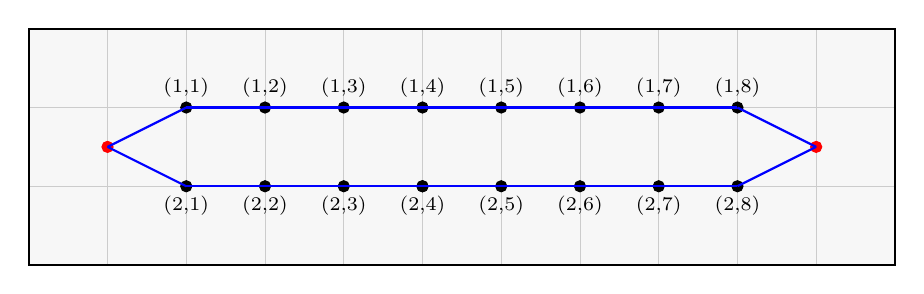
\begin{tikzpicture}% [scale=0.8] 
\draw[step=1cm, very thin, gray!40] (0,0) grid (11,3);
\draw[black, thick] (0,0) rectangle (11,3);
\filldraw [red] (1,1.5) circle (2pt);
\filldraw [red] (10,1.5) circle (2pt);
\foreach \i in {2}
{
\filldraw [black] (2,\i) circle (2pt);
\filldraw [black] (3,\i) circle (2pt);
\filldraw [black] (4,\i) circle (2pt);
\filldraw [black] (5,\i) circle (2pt);
\filldraw [black] (6,\i) circle (2pt);
\filldraw [black] (7,\i) circle (2pt);
\filldraw [black] (8,\i) circle (2pt);
\filldraw [black] (9,\i) circle (2pt);
}

\filldraw [black] (2,1) circle (2pt);
\filldraw [black] (3,1) circle (2pt);
\filldraw [black] (4,1) circle (2pt);
\filldraw [black] (5,1) circle (2pt);
\filldraw [black] (5,1) circle (2pt);
\filldraw [black] (6,1) circle (2pt);
\filldraw [black] (7,1) circle (2pt);
\filldraw [black] (8,1) circle (2pt);
\filldraw [black] (9,1) circle (2pt);
\draw[thick, blue] (1,1.5) -- (2,1);
\draw[thick, blue] (1,1.5) -- (2,2);
\draw[thick, blue] (2,2) -- (3,2);
\draw[thick, blue] (2,1) -- (3,1);
\draw[thick, blue] (3,1) -- (4,1);
\draw[thick, blue] (3,2) -- (4,2);
\draw[thick, blue] (4,1) -- (5,1);
\draw[thick, blue] (4,2) -- (5,2);
\draw[thick, blue] (5,2) -- (6,2);
\draw[thick, blue] (5,1) -- (6,1);
\draw[thick, blue] (6,2) -- (7,2);
\draw[thick, blue] (6,1) -- (7,1);
\draw[thick, blue] (7,1) -- (8,1);
\draw[thick, blue] (7,2) -- (8,2);
\draw[thick, blue] (8,1) -- (9,1);
\draw[thick, blue] (8,2) -- (9,2);
\draw[thick, blue] (9,1) -- (10,1.5);
\draw[thick, blue] (9,2) -- (10,1.5);

\node[anchor=north,font=\scriptsize] at (2,1) {(2,1)};
\node[anchor=north,font=\scriptsize] at (3,1) {(2,2)};
\node[anchor=north,font=\scriptsize] at (4,1) {(2,3)};
\node[anchor=north,font=\scriptsize] at (5,1) {(2,4)};
\node[anchor=north,font=\scriptsize] at (6,1) {(2,5)};
\node[anchor=north,font=\scriptsize] at (7,1) {(2,6)};
\node[anchor=north,font=\scriptsize] at (8,1) {(2,7)};
\node[anchor=north,font=\scriptsize] at (9,1) {(2,8)};
\node[anchor=south,font=\scriptsize] at (2,2) {(1,1)};
\node[anchor=south,font=\scriptsize] at (3,2) {(1,2)};
\node[anchor=south,font=\scriptsize] at (4,2) {(1,3)};
\node[anchor=south,font=\scriptsize] at (5,2) {(1,4)};
\node[anchor=south,font=\scriptsize] at (6,2) {(1,5)};
\node[anchor=south,font=\scriptsize] at (7,2) {(1,6)};
\node[anchor=south,font=\scriptsize] at (8,2) {(1,7)};
\node[anchor=south,font=\scriptsize] at (9,2) {(1,8)};

% \draw[very thick] (3,1) -- (3,2);
% \draw[very thick] (4,1) -- (4,2);
% \draw[very thick] (7,1) -- (7,2);
% \draw[very thick] (7,1) -- (7,2);
% \draw[very thick] (8,1) -- (8,2);
% \draw[very thick] (9,1) -- (9,2);
\begin{pgfonlayer}{background}
    \filldraw [line width=4mm,black!3]
      (0.2,0.2)  rectangle (10.8,2.8);
  \end{pgfonlayer}
\end{tikzpicture}
%\vskip-0.2cm
  \caption{
 Non-crossing partition
 of $2 \times d$ with $d=8$.} 
\label{f3-1-2-20}
\end{figure}

\vskip-0.4cm

\noindent
which yields a term of order
$$
p_m^{2d+2} (m(m-1))^d
=
p_m^{2d+2} m^d \sum_{l=0}^d {d \choose l} (-1)^l m^{d-l} 
$$ 
 which is compensated by the term 
$$ 
 ( \E_m [ \sigma_k (t) ] )^2 = 
p_m^{2d+2} m^{2d} \frac{((kr-t) / r)^{2d}}{(d!)^2} 
$$
obtained from \eqref{fjkdls-0} as
$$
p_m^{2d+2} (m(m-1))^d
- p_m^{2d+2} m^{2d} 
=
p_m^{2d+2} \sum_{l=1}^d {d \choose l} (-1)^l m^{2d-l}, 
$$ 
 hence the dominant term in $\Var_m [ \sigma_k (t) ]$ is
 given by the partition of Figure~\ref{f3-1-2-30} 
 
\begin{figure}[H]
\centering 
  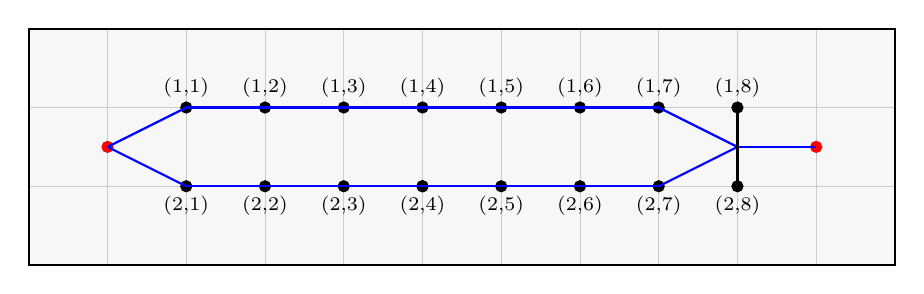
\begin{tikzpicture}% [scale=0.8] 
\draw[step=1cm, very thin, gray!40] (0,0) grid (11,3);
\draw[black, thick] (0,0) rectangle (11,3);
\filldraw [red] (1,1.5) circle (2pt);
\filldraw [red] (10,1.5) circle (2pt);
\foreach \i in {2}
{
\filldraw [black] (2,\i) circle (2pt);
\filldraw [black] (3,\i) circle (2pt);
\filldraw [black] (4,\i) circle (2pt);
\filldraw [black] (5,\i) circle (2pt);
\filldraw [black] (6,\i) circle (2pt);
\filldraw [black] (7,\i) circle (2pt);
\filldraw [black] (8,\i) circle (2pt);
\filldraw [black] (9,\i) circle (2pt);
}

\filldraw [black] (2,1) circle (2pt);
\filldraw [black] (3,1) circle (2pt);
\filldraw [black] (4,1) circle (2pt);
\filldraw [black] (5,1) circle (2pt);
\filldraw [black] (5,1) circle (2pt);
\filldraw [black] (6,1) circle (2pt);
\filldraw [black] (7,1) circle (2pt);
\filldraw [black] (8,1) circle (2pt);
\filldraw [black] (9,1) circle (2pt);
\draw[thick, blue] (1,1.5) -- (2,1);
\draw[thick, blue] (1,1.5) -- (2,2);
\draw[thick, blue] (2,2) -- (3,2);
\draw[thick, blue] (2,1) -- (3,1);
\draw[thick, blue] (3,1) -- (4,1);
\draw[thick, blue] (3,2) -- (4,2);
\draw[thick, blue] (4,1) -- (5,1);
\draw[thick, blue] (4,2) -- (5,2);
\draw[thick, blue] (5,2) -- (6,2);
\draw[thick, blue] (5,1) -- (6,1);
\draw[thick, blue] (6,2) -- (7,2);
\draw[thick, blue] (6,1) -- (7,1);
\draw[thick, blue] (7,1) -- (8,1);
\draw[thick, blue] (7,2) -- (8,2);
\draw[thick, blue] (8,1) -- (9,1.5);
\draw[thick, blue] (8,2) -- (9,1.5);
\draw[thick, blue] (9,1.5) -- (10,1.5);

\draw[very thick] (9,1) -- (9,2);

\node[anchor=north,font=\scriptsize] at (2,1) {(2,1)};
\node[anchor=north,font=\scriptsize] at (3,1) {(2,2)};
\node[anchor=north,font=\scriptsize] at (4,1) {(2,3)};
\node[anchor=north,font=\scriptsize] at (5,1) {(2,4)};
\node[anchor=north,font=\scriptsize] at (6,1) {(2,5)};
\node[anchor=north,font=\scriptsize] at (7,1) {(2,6)};
\node[anchor=north,font=\scriptsize] at (8,1) {(2,7)};
\node[anchor=north,font=\scriptsize] at (9,1) {(2,8)};
\node[anchor=south,font=\scriptsize] at (2,2) {(1,1)};
\node[anchor=south,font=\scriptsize] at (3,2) {(1,2)};
\node[anchor=south,font=\scriptsize] at (4,2) {(1,3)};
\node[anchor=south,font=\scriptsize] at (5,2) {(1,4)};
\node[anchor=south,font=\scriptsize] at (6,2) {(1,5)};
\node[anchor=south,font=\scriptsize] at (7,2) {(1,6)};
\node[anchor=south,font=\scriptsize] at (8,2) {(1,7)};
\node[anchor=south,font=\scriptsize] at (9,2) {(1,8)};

% \draw[very thick] (3,1) -- (3,2);
% \draw[very thick] (4,1) -- (4,2);
% \draw[very thick] (7,1) -- (7,2);
% \draw[very thick] (7,1) -- (7,2);
% \draw[very thick] (8,1) -- (8,2);
% \draw[very thick] (9,1) -- (9,2);
\begin{pgfonlayer}{background}
    \filldraw [line width=4mm,black!3]
      (0.2,0.2)  rectangle (10.8,2.8);
  \end{pgfonlayer}
\end{tikzpicture}
%\vskip-0.2cm
  \caption{
 Non-crossing partition
 of $2 \times d$ with $d=8$.} 
\label{f3-1-2-30} 
\end{figure}

\vskip-0.4cm

\noindent
 which yields 
$$
 \Var_m [ \sigma_k (t) ]
 \sim 
 4^{d-1}
 p_m^{2d+1}
(m(m-1))^{d-1}m 
 \int_{
    [0,r]^{2d} 
  }\left(\bigotimes_{i=1}^2
 u_t \right)_{\! \! \! \rho}
 ( x_1, \ldots , x_{2d} ) 
 \mu_{\bar{\rho}_1} ( d x_1 ) 
 \cdots
 \mu_{\bar{\rho}_{2d}} ( d x_{2d} ) 
, 
$$ 
 where we used the relation
\begin{align} 
\nonumber 
  \sum_{j_0 + j_1 = d-l\atop j_0,j_1\geq 0}
      {2j_0\choose j_0}
      {2j_1\choose j_1} 
& = 4^{d-1}, 
\end{align} 
 with
$$ 
 \int_{
    [0,r]^{2d}
 }\left(
 u_t
 \otimes
 u_t
 \right)_{ \rho}
 ( x_1, \ldots , x_{2d} ) 
 \mu_{\bar{\rho}_1} ( d x_1 ) 
 \cdots
 \mu_{\bar{\rho}_{2d}} ( d x_{2d} ) 
=
\frac{((kr-t) /r)^{2d-1}}{(2d-1)!}
.
$$
 If $m^{-1} \gg p_m$, the term 
$$ 
 ( \E_m [ \sigma_k (t) ] )^2 = 
p_m^{2d+2} m^{2d} \frac{((kr-t) / r)^{2d}}{(d!)^2}, 
$$ 
 is dominated by the $d$-block partition 
 given by the partition of Figure~\ref{f3-1-2-40} 

 % \vskip-0.2cm

\begin{figure}[H]
\centering 
  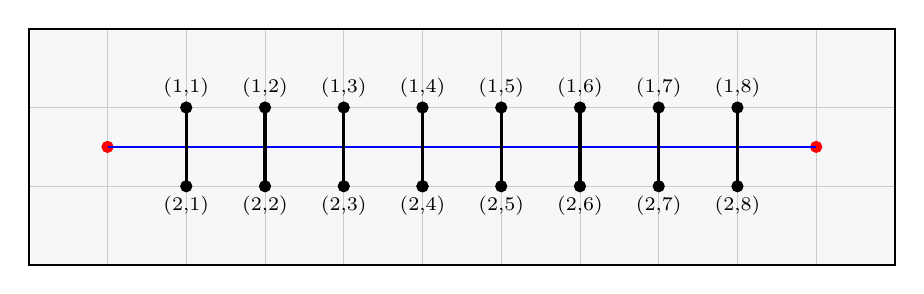
\begin{tikzpicture}% [scale=0.8] 
\draw[step=1cm, very thin, gray!40] (0,0) grid (11,3);
\draw[black, thick] (0,0) rectangle (11,3);
\filldraw [red] (1,1.5) circle (2pt);
\filldraw [red] (10,1.5) circle (2pt);
\foreach \i in {2}
{
\filldraw [black] (2,\i) circle (2pt);
\filldraw [black] (3,\i) circle (2pt);
\filldraw [black] (4,\i) circle (2pt);
\filldraw [black] (5,\i) circle (2pt);
\filldraw [black] (6,\i) circle (2pt);
\filldraw [black] (7,\i) circle (2pt);
\filldraw [black] (8,\i) circle (2pt);
\filldraw [black] (9,\i) circle (2pt);
}

\filldraw [black] (2,1) circle (2pt);
\filldraw [black] (3,1) circle (2pt);
\filldraw [black] (4,1) circle (2pt);
\filldraw [black] (5,1) circle (2pt);
\filldraw [black] (5,1) circle (2pt);
\filldraw [black] (6,1) circle (2pt);
\filldraw [black] (7,1) circle (2pt);
\filldraw [black] (8,1) circle (2pt);
\filldraw [black] (9,1) circle (2pt);
\draw[thick, blue] (1,1.5) -- (2,1.5);
\draw[thick, blue] (1,1.5) -- (2,1.5);
\draw[thick, blue] (2,1.5) -- (3,1.5);
\draw[thick, blue] (3,1.5) -- (4,1.5);
\draw[thick, blue] (4,1.5) -- (5,1.5);
\draw[thick, blue] (5,1.5) -- (6,1.5);
\draw[thick, blue] (6,1.5) -- (7,1.5);
\draw[thick, blue] (7,1.5) -- (8,1.5);
\draw[thick, blue] (8,1.5) -- (9,1.5);
\draw[thick, blue] (9,1.5) -- (10,1.5);

\node[anchor=north,font=\scriptsize] at (2,1) {(2,1)};
\node[anchor=north,font=\scriptsize] at (3,1) {(2,2)};
\node[anchor=north,font=\scriptsize] at (4,1) {(2,3)};
\node[anchor=north,font=\scriptsize] at (5,1) {(2,4)};
\node[anchor=north,font=\scriptsize] at (6,1) {(2,5)};
\node[anchor=north,font=\scriptsize] at (7,1) {(2,6)};
\node[anchor=north,font=\scriptsize] at (8,1) {(2,7)};
\node[anchor=north,font=\scriptsize] at (9,1) {(2,8)};
\node[anchor=south,font=\scriptsize] at (2,2) {(1,1)};
\node[anchor=south,font=\scriptsize] at (3,2) {(1,2)};
\node[anchor=south,font=\scriptsize] at (4,2) {(1,3)};
\node[anchor=south,font=\scriptsize] at (5,2) {(1,4)};
\node[anchor=south,font=\scriptsize] at (6,2) {(1,5)};
\node[anchor=south,font=\scriptsize] at (7,2) {(1,6)};
\node[anchor=south,font=\scriptsize] at (8,2) {(1,7)};
\node[anchor=south,font=\scriptsize] at (9,2) {(1,8)};

\draw[very thick] (2,1) -- (2,2);
\draw[very thick] (3,1) -- (3,2);
\draw[very thick] (4,1) -- (4,2);
\draw[very thick] (5,1) -- (5,2);
\draw[very thick] (6,1) -- (6,2);
\draw[very thick] (7,1) -- (7,2);
\draw[very thick] (7,1) -- (7,2);
\draw[very thick] (8,1) -- (8,2);
\draw[very thick] (9,1) -- (9,2);
\begin{pgfonlayer}{background}
    \filldraw [line width=4mm,black!3]
      (0.2,0.2)  rectangle (10.8,2.8);
  \end{pgfonlayer}
\end{tikzpicture}
%\vskip-0.2cm
 \caption{
 Non-crossing partition of $2 \times d$ with $d=8$.} 
\label{f3-1-2-40} 
\end{figure}

\vskip-0.4cm

\noindent
 which yields 
$$ 
 \Var_m [ \sigma_k (t) ]
 \sim 
p_m^{d+1}
 m^d(m-1)^d 
 \int_{
    [0,r]^{2d} 
  }\left(\bigotimes_{i=1}^2
 u_t \right)_{\! \! \! \rho}
 ( x_1, \ldots , x_{2d} ) 
 \mu_{\bar{\rho}_1} ( d x_1 ) 
 \cdots
 \mu_{\bar{\rho}_{2d}} ( d x_{2d} ) 
, 
$$ 
 with
$$ 
 \int_{
    [0,r]^{2d}
 }\left(
 u_t
 \otimes
 u_t
 \right)_{ \rho}
 ( x_1, \ldots , x_{2d} ) 
 \mu_{\bar{\rho}_1} ( d x_1 ) 
 \cdots
 \mu_{\bar{\rho}_{2d}} ( d x_{2d} ) 
=
\frac{((kr-t) /r)^d}{d!}
.
$$
\end{Proof} 
\begin{corollary}
  \label{cjkfl} 
% Suppose that $\limsup_{m\to \infty} p_m < 1$.
  For $m$ large enough, % $n\geq 4(v(G)-1)$,
  the $n$-th cumulant of the normalized $k$-hop count
$$
  \widebar{\sigma}_k (t):= \frac{\sigma_k (t)-\E_m [ \sigma_k (t)]}{\sqrt{\Var_m [ \sigma_k (t) ]}}
  $$ 
 satisfies 
  \begin{eqnarray*}
    \kappa_n\left(\widebar{\sigma}_k (t)\right)\leq \begin{cases}
      \displaystyle
      \frac{n!^{d+1}}{(C m p_m)^{n/2-1}}~~~~~~~{when}~~~p_m \gg m^{-(d-1)/d},
      \medskip
      \\
      \displaystyle
      \frac{n!^{d+1}}{\big(C m^d p_m^{d+1}\big)^{n/2-1}}~~~~{when}~~~p_m\ll m^{-1},
    \end{cases}
\end{eqnarray*}
 $n\ge3$, where $C$ is a constant independent of $m \geq 1$.
\end{corollary}
\begin{Proof}
% From the inequality $\sqrt{2\pi j}({j}/{e})^j<j!$, we have
% \begin{equation} j^{j-1}<\frac{(j-1)!}{\sqrt{2\pi j}}e^j. \end{equation}
  When $p_m \gg m^{-(d-1)/d}$, from the inequalities  
  \eqref{low-1} and \eqref{upp-1}, we have 
  \begin{align*}
    \nonumber
    \kappa_n\left(\widebar{\sigma}_k (t)\right)&= \frac{\kappa_n(\sigma_k (t))}{\Var_m [ \sigma_k (t) ]^{n/2}}    \\
    \nonumber
    &\leq n!^d n^{n-1}m^{1+(d-1)n}p_m^{nd+1}
      \left(  
\frac{p_m^{2d+1} m^{2d-1} (2 (kr-t) /r)^{2d-1}}{2(2d-1)!}
      \right)^{-n/2}
    \\
    \nonumber
    &\leq n!^{d+1} e^n m^{1-n/2}p_m^{nd+1}
    \left(  
 \frac{p_m^{2d+1} (2 (kr-t) /r)^{2d-1}}{2(2d-1)!}
      \right)^{-n/2}
    \\
    \nonumber
    & = n!^{d+1} e^n m^{1-n/2} p_m^{1-n/2}
    \left(  
\frac{(2 (kr-t) /r)^{2d-1}}{2(2d-1)!}
      \right)^{-n/2}. 
\end{align*}
  Similarly, when $p_m\ll m^{-1}$ from,  
  % , from the inequality $$  \frac{m!}{(m-d)!}\ge (m-d+1)^d=\left(1-\frac{d-1}m\right)^dm^d \ge \left( \frac{3m}{4} \right)^d $$ and
  \eqref{low-2} and \eqref{upp-2} we have 
  \begin{align*}
    \kappa_n\left(\widebar{\sigma}_k (t)\right)&= \frac{\kappa_n(\sigma_k (t))}{\Var_m [\sigma_k (t)]^{n/2}}\nonumber\\
    &\leq n!^d n^{n-1} m^d p_m^{2n+d-1}
      \left(  
    Cm^dp_m^{d+1}\right)^{-n/2}\nonumber\\
    &= n^{n-1}n!^d m^d p_m^{d-1}
      \left(
    C m^d p_m^{d-1}\right)^{-n/2}\nonumber\\
    &\leq \frac{(n-1)!}{\sqrt{2\pi n}}e^nn!^d m^d p_m^{d-1}
      \left(C
    \left(\frac{3m}{4}\right)^d p_m^{d-1}\right)^{-n/2}\nonumber\\
      &\leq e^nn!^{d+1} m^d p_m^{d+1}
        \left(C
        \left(\frac{3m}{4} \right)^d p_m^{d+1}\right)^{-n/2}
        \nonumber\\
        &= \frac{n!^{d+1}e^n }{\big(m^d p_m^{d+1}\big)^{(n-2)/2}} 
                \left(C
                \left(\frac{3}{4} \right)^d \right)^{-n/2}
                .
\end{align*}
\end{Proof}

\section{Berry-Esseen bounds and moderate deviations} % Central limit theorem} 
\label{sec8} 

\begin{remark}
  To ensure a normal approximation, we only need to let some
  $m_\ell$ tend to infinity,
  i.e.
  % $M$ tends to infinity,
  $\max_{1\leq \ell \leq d} m_\ell$ should tend to infinity,   
  which does not require 
  $m_1=\cdots=m_{k-1}=m$ with $m$ tending to infinity. 
\end{remark}
 Given $k\geq 2$ and $t\in [(k-1)r,kr)$,
 we consider the normalized $k$-hop count
$$
\widebar{\sigma}_k^{(m)} (t):= \frac{\sigma_k^{(m)} (t)- \E_\lambda [\sigma_k(t)]}{\sqrt{\Var_\lambda  [ \sigma_k(t)]}}. 
$$
 For any $t \in [(k-1)r,kr)$, from Corollary~\ref{cjkfl} the skewness
 of $\sigma_k (t )$ satisfies  
  \begin{eqnarray*}
    \kappa_3\left(\widebar{\sigma}_k (t)\right)\leq \begin{cases}
      \displaystyle
      (C m p_m)^{-1/2}~~~~~~~{when}~~~pm \gg m^{-1+1/d},
      \medskip
      \\
      \displaystyle
      (C m^d p_m^{d+1})^{-1/2}~~~~{when}~~~p_m\ll m^{-1},
    \end{cases}
\end{eqnarray*}
 for $m$ large enough, where $C$ is a constant independent of $m \geq 1$, 
  and more generally,
  from Corollary~\ref{cjkfl} and Theorem~1 in \cite{Janson1988}, 
  we find that 
 $\widebar{\sigma}_k^{(m)} (t)$
 converges in distribution
 to the standard normal distribution ${\cal N}(0,1)$ as $\lambda$
 tends to infinity, 
 provided that $p_m \gg m^{-1+1/d}$ as $m$ tends to
 infinity.

 \medskip
 
 From Corollary~\ref{cjkfl}, we check that if
 $p_m \gg m^{-1+1/d}$, the cumulants of the normalized
 $U$-statistics 
 $\widebar{\sigma}_k (t)$ satisfy the Statulevi\v{c}ius growth condition 
 \eqref{Statuleviciuscond2} with $\gamma := d$ and 
 $$
 \Delta_m := 
 (C m p_m)^{1/2}, 
$$ 
      where $C>0$ depends only on
      $d \geq 2$.
 Therefore, from Proposition~\ref{l1}-$i)$
 we have the following results.
\begin{corollary}
\label{thm4.2-1}
(Kolmogorov bound). 
% Let $f:[0,r]^d \to\real$ be a measurable function satisfying Assumption~\ref{assu1}, with $d\geq 2$.
    % Denote $W:=\frac{S_{n,k}(f)-\kappa_1(S_{n,k}(f))}{\sqrt{\kappa_2(S_{n,k}(f))}}$,
 Let $d\geq 2$, $t\in [(k-1)r,kr]$, and assume that $p_m \gg m^{-1+1/d}$.
  Then, for $m$ large enough, we have 
    \begin{equation}
    \label{fjkf}
      \sup_{x\in\real}\left|
      \P_m \left(
      \widebar{\sigma}_k (t) \leq x\right)-\Phi(x)\right|\leq \frac{C_d}{(m p_m)^{1/(2+4d)}},
    \end{equation}
    where $C_d>0$ depends only on
    $d \geq 2$. 
\end{corollary}
In particular, if
 $p_m \sim m^{-\alpha}$ with $\alpha \in [0,1 - 1/d)$, we find 
    \begin{equation}
\nonumber % \label{fjkf}
      \sup_{x\in\real}\left|
      \P_m \left(
      \widebar{\sigma}_k (t) \leq x\right)-\Phi(x)\right|\leq \frac{C_d}{m^{(1+\alpha )/(2+4d)}},
    \end{equation}
    where $C_d>0$ depends only on
    $d \geq 2$.
% \noindent 
 In the case $d=1$, \eqref{d=1} 
 the central limit Berry-Esseen rate holds
 since $\sigma_2(t)$ has a binomial distribution
 with parameter \eqref{d=1}.

 \medskip

 The following threshold result for $k$-hop containment
 is a another direct consequence of Theorem~\ref{th7.5-1}. 
\begin{corollary}
\label{graphcontain}
    Let $d\geq 2$ and $t\in [(k-1)r,kr]$. 
    We have 
    \begin{enumerate}[a)]
      \item $\lim_{m\to\infty}\P_m (\sigma_k (t) \geq 1)=1$ if $p_m\gg m^{-1+1/d}$, 
      \item $\lim_{m\to\infty}\P_m (\sigma_k (t) =0)=1$ if $p_m\ll m^{-1}$. 
    \end{enumerate}
  \end{corollary}
  \begin{Proof}
 When $p_m\gg m^{-1+1/d}$,
 from \eqref{upp-1} we have % and \eqref{upp-2}, we have 
 \begin{equation}
   \nonumber
   |\kappa_2(\sigma_k (t))|\leq
   2^{d+1} m^{2d-1}p_m^{2d+1},
 \end{equation}
 hence by \eqref{fjkdls-0} we have 
\begin{equation}
\nonumber
      \lim_{m\to \infty}
   \frac{\kappa_2(\sigma_k (t) )}{\kappa_1(\sigma_k (t) )^2} \lesssim 
\lim_{m\to \infty}
   \frac{m^{2d-1}p_m^{2d+1}}{p_m^{2d+2}m^{2d}}
   = 0, % \to0,
 \end{equation}
 and
 \begin{eqnarray}
   \lim_{m\to \infty}
   \frac{(\E_m [\sigma_k (t) ])^2}{\E_m [(\sigma_k (t) )^2]}
   =
   \lim_{m\to \infty} \frac{\kappa_1(\sigma_k (t) )^2}{\kappa_2(\sigma_k (t) )+\kappa_1(\sigma_k (t) )^2}
   = 1.
 \end{eqnarray}
 On the other hand, if $p_m\ll m^{-1}$, from
  \eqref{fjkdls-0} we have 
 \begin{equation}
\nonumber
    \lim_{m\to \infty} \E_m  [ \sigma_k (t)  ] =0. % \kappa_1(N_G)\to 0,
 \end{equation}
 We conclude by the first and second moment methods,
 see \cite[Page~54]{JLR}, which state that 
\begin{equation}
\nonumber % \label{firstsecm}
\frac{(\E_m [\sigma_k (t) ])^2}{\E_m [( \sigma_k (t) )^2]}\le\P_m (\sigma_k (t) >0)\leq \E_m [\sigma_k (t) ]. 
\end{equation}
% for any non-negative integer-valued random variable $X$. With $X=N_G$,
\end{Proof}
 In the special case where
 any two nodes are connected whenever they
 are located within the distance $r$,
 i.e. in the random geometric graph setting,
 Corollary~\ref{thm4.2-1} can be improved into 
 a Berry-Esseen bound 
 as in the following remark that follows from e.g. 
% note that $\widebar{\sigma}_k(n)$ admits a Hoeffding decomposition and
 Theorem~4.1 of \cite{PS4} or 
 Theorem~2.1 of \cite{zhangzs}
 for the Kolmogorov distance. 
\begin{remark}
% \label{fsklf34}
 Let $d\geq 2$ and $t\in [(k-1)r,kr]$. 
 Assume that $p_m = 1$, $m\geq 1$,
  and
  $\mu_1 =\cdots = \mu_d$. 
  We have the Kolmogorov distance bound 
  $$
  \sup_{x\in\real }|\P_m (\widebar{\sigma}_k (t)
   \leq x)-\Phi(x)|
  \leq \frac{C_k}{\sqrt{m}}, \qquad
  m \geq 1,
  $$
  % where $d_K(\widebar{\sigma}_k (t), {\cal N})$ denotes the Kolmogorov % Wasserstein  distance between  $\widebar{\sigma}_k (t)$ and the standard normal distribution ${\cal N}$, and
  where $C_k>0$ is a constant.
\end{remark}
 By Corollary~\ref{cjkfl} and Proposition~\ref{l1}-$ii)$,
 we also have the following moderate deviation result.
\begin{corollary}
% \label{corg2-0}
 (Moderate deviation principle).
% Let $f:[0,r]^d \to\real$ be a measurable function satisfying Assumption~\ref{assu1}, with $d\geq 2$.
    % Denote $W:=\frac{S_{n,k}(f)-\kappa_1(S_{n,k}(f))}{\sqrt{\kappa_2(S_{n,k}(f))}}$,
  Let $d\geq 2$ and $t\in [(k-1)r,kr]$, 
  let $( a_m)_{m \geq 1}$ be a sequence of real numbers tending to infinity, and such that 
$ 
  a_m \ll m^{1/(2+4 d)}$. 
   % as $n\to\infty$.
  Then, $\big(a_m^{-1} \widebar{\sigma}_k (t) \big)_{m \geq 1}$ satisfies a moderate deviation principle with speed $a_m^2$ and rate function $x^2/2$. 
\end{corollary} 
\section{Poisson approximation}\label{sec-pol}
To study the Poisson approximation of the $k$-hop count $W$, we employ the
well-established Stein-Chen method developed in 
 \cite{chen1975} for deriving bounds on the distance between a distribution of interest and the Poisson distribution under various probability metrics. The method is based on the key observation that a non-negative random variable $Y \sim \Pn(\lambda)$ if and only if 
$$\E[\lambda f(Y+1)-Yf(Y)]=0,$$
for all bounded functions $f:\Z_+\to\R$. 
This characterization yields the following Stein identity for Poisson approximation: for any $j\ge0$, 
\begin{equation}
  \label{steinidP}
  \lambda f(j+1)-jf(j)=h(j)-\Pn(\lambda)\{h\},
\end{equation}
where $\Pn(\lambda)\{h\}:=\E_m [ h(Y)]$ with $Y\sim \Pn(\lambda)$.

\medskip

 In order to apply the Stein-Chen method, we first recall some background on size-bias coupling from \cite{LiuXia20}.
 Size biasing has attracted considerable attention for many decades
(see \cite{BarbourHolstJanson}, \cite{nross}, \cite{AGK19} and the references therein).
In the case of sums of Bernoulli random variables, the size-biased
distribution admits a particularly simple form. 
Consider 
\begin{itemize}
\item
 a family $\{X_i : i \in \ci\}$ of Bernoulli random variables such that 
 $\P_m (X_i = 1) = \bar{p}_i$,
\item
  a family
  $\{\{X_j^{(i)} : j \in \ci\} : i \in \ci\}$ 
  of Bernoulli random variables such that 
$$
   \law\!\big(\{X_j^{(i)} : j \in \ci\}\big)
   = \law\!\big(\{X_j : j \in \ci\} \,|  \, X_i = 1\big), 
$$
 \item a random index $B$, independent of
$\{\{X_j^{(i)} : j \in \ci\} : i \in \ci\}$, with distribution 
  $$\P_m (B = i) = \frac{\bar{p}_i}{\E_m  [W]},
  \quad i \in \ci.
  $$ 
\end{itemize} 
The size-biased version of 
$$W := \sum_{i \in \ci} X_i$$
 is defined as 
 \begin{equation}
   \nonumber % \label{sizebiasing}
 W^s := 1 + \sum_{j \ne B} X_j^{(B)}. 
\end{equation}
\begin{definition}[\cite{BarbourHolstJanson}]
The family $\{X_i : i \in \ci\}$ is said to be
\emph{negatively related} (resp. \emph{positively related}) if one can
construct $\{\{X_j^{(i)} : j \in \ci\} : i \in \ci\}$ such that
$X_j^{(i)} \le X_j$ (resp. $X_j^{(i)} \ge X_j$) for all $j \ne i$.
\end{definition}
When $\{X_i\}$ are negatively related, we have 
\begin{equation}
  \nonumber % \label{monotonecoupling1}
   \E\lvert W + 1 - W^s\rvert
   = \E_m  [ W + 1 - W^s ] 
   = \mu^{-1}(\mu - \sigma^2),
\end{equation}
where $\mu = \E_m [W]$ and $\sigma^2 = \var(W)$.
 On the other hand, if $\{X_i\}$ are positively related, then
\begin{align}\label{monotonecoupling2}
   \E_m [\lvert W + 1 - W^s\rvert ]
   &= \E_m  \bigg[\bigg|\sum_{j \ne B} (X_j^{(B)} - X_j) - X_B\bigg|
     \bigg]
   \nonumber\\
   &\le \E_m  \bigg[
     \sum_{j \ne B} (X_j^{(B)} - X_j) + X_B\bigg] \nonumber\\
   &= \E_m  [ W^s - W - 1 ] + 2\mu^{-1} \sum_{i \in \ci} \bar{p}_i^2 \nonumber\\
   &= \mu^{-1}(\sigma^2 - \mu) + 2\mu^{-1} \sum_{i \in \ci} \bar{p}_i^2.
\end{align}
% \subsubsection*{Stein-Chen method}
 In what follows, we consider 
 the family
        $\{I_\beta \}_{\beta \in [m_1]\times\cdots\times[m_d]}$
 of Bernoulli random variables
 appearing  in \eqref{ustat} and defined as 
\begin{equation}
          \label{ibeta}
          I_\beta : =
          Y^{(0)}_{\beta (1)}Y^{(1)}_{\beta (1),\beta (2)}\cdots Y^{(d-1)}_{\beta (d-1),\beta (d)}
 Y^{(d)}_{\beta (d)}
 {\bf1}_{\big\{U^{(1)}_{\beta (1)} \leq \cdots \leq U^{(d)}_{\beta (d)} \leq kr-t \big\}},
        \quad
        \beta \in [m_1]\times\cdots\times[m_d]. 
\end{equation} 
 Next, we investigate the conditional distribution of $W$ given $I_\alpha=1$, denoted by $\law(W|I_\alpha=1)$, for arbitrary 
$\alpha\in[m_1]\times\cdots\times[m_d]$.
\begin{prop}
	\label{coupling-1}
        The family
        of Bernoulli random variables
        $\{I_\beta \}_{\beta \in [m_1]\times\cdots\times[m_d]}$
        is positively related. 
\end{prop}
\begin{Proof}
 We consider the size-bias coupling of 
 $\{I_\alpha\}_{\alpha\in\ci}$
 defined as follows.
 For each $\alpha\in\ci$, let the Bernoulli random variables $\{I_\beta^{(\alpha)}\}_{\beta\in\ci,\beta\ne\alpha}$ be defined as follows.
\begin{enumerate}
\item 
For $\beta\in\ci$ such that $\beta(\ell)\ne\alpha(\ell)$ for all $\ell=1,\dots,d,$ we take
$I_\beta^{(\alpha)}:=I_{\beta}$. 
\item For $\beta\in\ci$ with some $A\subsetneq [d]$ such that $\beta(i)=\alpha(i)$ iff $i\in A$, we define 
\begin{equation}
\nonumber
   	I_{\beta}^{(\alpha)}:=
	\widetilde{Y}_{\beta(1),\beta(2)}\cdots\widetilde{Y}_{\beta(d-1),\beta(d)},
\end{equation}
where 
\begin{equation*}
	\widetilde{Y}_{0,\beta(1)}:=
	\begin{cases}1,\ \ \ &\mbox{if~} 1\in A;
          \medskip
          \\
	  Y_{\beta (1 )}^{(0)} 
,\ \ \ \ &\mbox{if~} 1\notin A,
	\end{cases}
\end{equation*}
\begin{equation*}
	\widetilde{Y}_{\beta(\ell),\beta(\ell+1)}:=\begin{cases}
	1,\ \ \ &\mbox{if}~\ell\in A \mbox{~and~} \ell+1\in A;
        \medskip
          \\
		Y_{\beta (\ell ),\beta (\ell + 1)}^{( \ell )}
                \bone_{\big\{ U_{\beta(\ell)}^{(\ell)} \leq U_{\beta(\ell+1)}^{(\ell+1)} \big\}},\ \ \ &\mbox{else},
	\end{cases}
\end{equation*}
for $\ell=1,\dots,d-1$,
and
\begin{equation*}
	\widetilde{Y}_{\beta(d),M}:=
	\begin{cases}1,\ \ \ &\mbox{if~} d\in A;
          \medskip
          \\
	  Y_{\beta (d)}^{(d)}
          \bone_{\big\{ U_{\beta( d )}^{( d )} \leq kr-t \big\}}
          ,\ \ \ \ &\mbox{if~} d\notin A.
	\end{cases}
\end{equation*}
\end{enumerate}
It is easy to verify that $\law(I_{\beta}^{(\alpha)})=\law\left(I_\beta\big|I_\alpha=1\right)$. In addition,
it is straightforward by construction
that $I_{\beta}^{(\alpha)}\ge I_\beta$, for all $\beta\ne\alpha$, and $\alpha\in\ci$.
\end{Proof} 
 For $\alpha\in\ci$, we denote $\underline{\alpha}:=\{\alpha(1),\dots,\alpha(d)\}$, and for $\alpha\in\ci$ fixed we define 
\begin{equation}
\nonumber
   	\nu(i):=|\{\beta\in\ci:|\underline{\beta}\cap\underline{\alpha}|=i\}|,~~~i=0,1,\dots,d.
\end{equation}
 We have 
\begin{align}\label{count-parti}
  \nu(i)&= \begin{cases}
    \displaystyle
    (m_1-1)\times(m_2-1)\times\cdots\times(m_d-1),\ \ \ &\mbox{\rm when~}i=0;\\
	\displaystyle
    	(m_1-1)(m_2-1)\cdots (m_d-1)\sum_{i=1}^d\frac1{m_i-1},\ \ \ &\mbox{when~}i=1;\\[0.5ex]
\displaystyle
    		(m_1-1)(m_2-1)\cdots (m_d-1)\sum_{1\le i\ne j\le d}\frac1{(m_i-1)(m_j-1)}, \ \ \ &\mbox{when~}i=2;\\[0.5ex]
		\ \ \ \ \ \vdots\\[0.5ex]
\displaystyle
    		\sum_{i=1}^d(m_i-1),\ \ \ &\mbox{when~}i=d-1;\\[0.5ex]
		1,\ \ \ &\mbox{when~}i=d.
	\end{cases}
\end{align}
For integer-valued random variables $X$ and $Y$, the total variation distance between $\law(X)$ and $\law(Y)$ is given by 
\begin{equation}
  \label{dtv}
  \dtv( X,Y):=\sup_{A\subseteq\Z}|\P_m (X\in A)-\P_m (Y\in A)|,
\end{equation}
 with $\Z:=\{0,\pm1,\pm2,\dots\}$ standing for the set of signed integers.
% \section{Poisson approximation}
\begin{theorem}\label{poi-thm}
  Let $d\geq 2$ and $t\in [(k-1)r,kr]$,
  and let $\sigma_k (t)=\sum_{\alpha\in\ci}I_\alpha$ be the $k$-hop count defined in
  \eqref{ustat}, with $I_\alpha$ given in
  \eqref{ibeta} and $\lambda (t):=\E_m  [ \sigma_k (t) ]>0$.
  Then, we have
\begin{align}
  \dtv(\sigma_k (t),\Pn(\lambda (t)))&\le
  \tilde{p}_m
  + 
  \sum_{i=1}^{d-1}\nu(i)p_m^{d+1-i},
  \label{po-error1}
\end{align}
where
\begin{equation}
\nonumber
     \tilde{p}_m:=\P_m (I_\alpha=1)
  =
  p_m^{d+1}
\int_0^{kr-t} \int_0^{x_d} \cdots \int_0^{x_2} \mu_1(dx_1)\cdots \mu_d(dx_d)
\end{equation}
 and $\nu(i)$ is given in \eqref{count-parti}.
\end{theorem}
\begin{Proof}
  In what follows, we let
  $W:  =\sigma_k (t)=\sum_{\alpha\in\ci}$
  and $\lambda: = \lambda (t)$.
  By the Stein-Chen method, we have 
\begin{align}
	\dtv( W ,\Pn(\lambda ))&= \sup_{A\subseteq \Z}|\P_m (W\in A)-\Pn(\lambda)\{A\}|\nonumber\\
				  &\le\sup_{A\subseteq \Z}|\E[\lambda f_A(W+1)-Wf_A(W)]|\label{steinest01}
\end{align}
where $f_A$ is the unique solution for $h(\cdot)=\bone(\cdot\in A)$ in \eqref{steinidP} with $f_A(0)=0$. Recall from \cite[Lemma~4.4]{nross}, for any $A\subseteq \Z$,
\begin{equation}
  \nonumber % \label{steinconst}
	\|f_A\|\le\min\{1,\lambda^{-1/2}\},~~~~\|\Delta f_A\|\le\frac{1-e^{-\lambda}}{\lambda}\le\lambda^{-1},
\end{equation}
where $\Delta f_A(j):=f_A(j+1)-f_A(j)$.
	From Proposition~\ref{coupling-1}, together with estimates in \eqref{monotonecoupling2}, we have
\begin{align}
\left|\E[\lambda f_A(W+1)-Wf_A(W)]\right|&= \left|\lambda\E[f_A(W+1)-f_A(W^s)]\right|\nonumber\\
				    &\le\lambda \|\Delta f_A\|\ \E|W+1-W^s|\nonumber\\
				    &\le\lambda^{-1}(\sigma^2 - \lambda) + 2\lambda^{-1} \sum_{\alpha \in \ci} (\P_m (I_\alpha=1))^2\nonumber\\
				    &=\lambda^{-1}(\sigma^2 - \lambda)+2\tilde{p}_m,\label{err01}
\end{align}
where $\sigma:=\Var(W)$. 
Moreover, we have 
\begin{align}
  \nonumber
  \sigma^2-\lambda&=\sum_{\alpha\in\ci}\sum_{\beta\in\ci}\cov(I_\alpha,I_\beta)-\sum_{\alpha\in\ci}\P_m (I_\alpha=1)
  \\
  \nonumber
  &=\sum_{\alpha\in\ci}\sum_{\beta\ne\alpha}\cov(I_\alpha,I_\beta)+\sum_{\alpha\in\ci}\cov(I_\alpha,I_\alpha)-\sum_{\alpha\in\ci}\P_m (I_\alpha=1)
  \\
  \nonumber
  &=\sum_{\alpha\in\ci}\sum_{\beta\ne\alpha}\cov(I_\alpha,I_\beta)-\sum_{\alpha\in\ci}(\P_m (I_\alpha=1))^2
  \\
  \label{err02}
  &=\sum_{\alpha\in\ci}\sum_{\beta\ne\alpha}\cov(I_\alpha,I_\beta)-\lambda\tilde{p}_m. 
\end{align}
For any $\alpha\ne\beta\in\ci$, if $\beta(i)\ne\alpha(i)$ for all $i=1,\dots,d$, then $I_\alpha$, $I_\beta$ are independent. For $\alpha\ne\beta\in\ci$ with $\beta(i)=\alpha(i)$ for some $i=1,\dots,d$, we have 
\begin{align}
  \nonumber
  \cov(I_\alpha,I_\beta)&=\E[I_\alpha I_\beta]-\tilde{p}_m^2
  \\
        \label{err03}
	&=\tilde{p}_m\E[I_\beta^{(\alpha)}]-\tilde{p}_m^2.
\end{align}
Let $\alpha\in\ci$ be fixed, for $\beta\ne\alpha$ with $|\underline{\beta}\cap\underline{\alpha}|=i$, $i=1,\dots,d-1$, we have 
\begin{equation}
  \nonumber 
	\E[I_{\beta}^{(\alpha)}]\le p_m^{d+1-i}.\label{err04}
\end{equation}
Collecting \eqref{count-parti}, 
\eqref{err03}, \eqref{err04} we have
\begin{align}
  \nonumber
  \sum_{\alpha\in\ci}\sum_{\beta\ne\alpha}\cov(I_\alpha,I_\beta)-\lambda\tilde{p}_m
  &=\sum_{\alpha\in\ci}\sum_{i=1}^{d-1}\sum_{\substack{\beta\in\ci\\|\underline{\beta}\cap\underline{\alpha}|=i}}\cov(I_\alpha,I_\beta)-\lambda\tilde{p}_m
  \\
  \nonumber
  &\le\sum_{\alpha\in\ci}\sum_{i=1}^{d-1}\sum_{\substack{\beta\in\ci\\|\underline{\beta}\cap\underline{\alpha}|=i}}\left(\tilde{p}_mp_m^{d+1-i}-\tilde{p}_m^2\right)-\lambda\tilde{p}_m
  \\
  \nonumber
  &\le\sum_{\alpha\in\ci}\sum_{i=1}^{d-1}\sum_{\substack{\beta\in\ci\\|\underline{\beta}\cap\underline{\alpha}|=i}}\tilde{p}_mp_m^{d+1-i}-\lambda\tilde{p}_m
  \\
  \nonumber
  &=\sum_{\alpha\in\ci}\sum_{i=1}^{d-1}\nu(i)\tilde{p}_mp_m^{d+1-i}-\lambda\tilde{p}_m
  \\
  \nonumber
  &=\lambda\sum_{i=1}^{d-1}\nu(i)p_m^{d+1-i}-\lambda\tilde{p}_m.\label{err05}
\end{align}
Combining 
\eqref{err01}, \eqref{err02} and \eqref{err05}, it shows that
\begin{align}
	\left|\E[\lambda f_A(W+1)-Wf_A(W)]\right|&\le\sum_{i=1}^{d-1}\nu(i)p_m^{d+1-i}+\tilde{p}_m
\end{align}
Combining with \eqref{steinest01}, the proof is complete. 
\end{Proof}
 We note that in order to ensure Poisson approximation, there is no need to force $\E_m  [\sigma_k (t)]$ to converge to a constant $\mu$. 
  Poisson approximation by Stein-Chen method does not require $\E_m  [\sigma_k (t)]$ be a constant. In fact, $\E_m  [\sigma_k (t)]$ can be large.
  \begin{corollary}
    \label{c2} 
    Let $d\geq 2$ and $t\in [(k-1)r,kr]$,
     and assume that $m_1=m_2=\cdots=m_d=m$,
  and assume that $m^dp_m^{d+1}\to c\in(0,\infty)$.
  Then, as $m$ tends to infinity we have
\begin{align}
  \dtv(\sigma_k (t),\Pn(\lambda))&
  \asymp m^{-1/(d+1)}.
\nonumber % \label{po-error1}
\end{align}
\end{corollary}
\begin{Proof}
  We have $\nu(i)\asymp m^{d-i}$,
   hence the error bound in \eqref{po-error1} is of order 
	$$\sum_{i=1}^{d-1}m^{d-i}p_m^{d+1-i}+p_m^{d+1}\asymp \sum_{i=1}^{d-1}m^{d-i}(m^{-\frac{d}{d+1}})^{d+1-i}\asymp m^{-1/(d+1)}.$$
\end{Proof}
 In the case $d=1$, 
 Poisson convergence also holds $\sigma_2(t)$ when
 $mp_m^2\to c\in(0,\infty)$ from
 \eqref{d=1}.

 \appendix

\section{Moments and cumulants} 
In this section we gather some preliminary facts 
on the relationships between joint moments, cumulants, and sums over partitions
that will be useful in the sequel. 
We let $\Pi[n]$ denote the set of partitions of $[n]:=\{1,\ldots , n\}$, 
 and given a symmetric function $f(\pi ) = f(\pi_1,\ldots , \pi_l)$ where
 $\pi = \{\pi_1,\ldots , \pi_l \} \in \Pi [n]$ is a partition of $\{1,\ldots , n\}$
 of size $l\geq 1$ we will use the notation 
$$
 \sum_{\pi \in \Pi [n]} f(\pi) = \sum_{l=1}^n \sum_{\pi_1\cup \cdots \cup \pi_l = \{1,\ldots , n\}}
 f(\{ \pi_1,\ldots , \pi_l \} ).
$$ 
 We will also use the M\"obius transform $\widehat{G}$ of a function $G$ on 
 partitions $\pi$ of $\{1,\ldots ,n\}$, defined as 
\begin{equation}
\label{g} 
 \widehat{G} (\sigma ) := \sum_{\pi \preceq \sigma } G(\pi ), 
 \qquad \sigma \in \Pi[n], 
\end{equation} 
 where the sum \eqref{g} runs over all partitions $\pi$ of 
 $\{1,\ldots ,n \}$ that are finer than $\sigma$,
 i.e. $\pi \preceq \sigma$. 
 The M\"obius inversion formula,
 see e.g. \cite{rotabk} or \S~2.5 of \cite{peccatitaqqu},
 states that the function $G$ in \eqref{g}
 can be recovered from its M\"obius transform
 $\widehat{G}$ as 
\begin{equation}
\label{bpi} 
 G(\pi) = \sum_{ \sigma \preceq \pi } \mu ( \sigma , \pi ) \widehat{G} (\sigma),  
\end{equation} 
 where $\mu ( \sigma , \pi )$ 
 is the M\"obius function, with 
 $\mu ( \sigma , \widehat{\bf 1} ) = (|\sigma |-1)! (-1)^{|\sigma |}$,
 where $|\sigma |$ denotes the cardinality of the
 block $\sigma \in \Pi [n]$ and 
 $\widehat{\bf 1} : = \{\{1,\ldots , n\}\}$ is 
 the one-block partition of $\{1,\ldots , n\}$. 
 By \eqref{g} and \eqref{bpi} we also have the relation  
\begin{equation}
\nonumber % \label{fjlksa1} 
 G(\pi)
 = \sum_{ \sigma \preceq \pi } \mu ( \sigma , \pi )
 \sum_{\eta \preceq \sigma } G(\eta ) 
 = \sum_{ \eta \preceq \sigma \preceq \pi } 
 \mu ( \sigma , \pi ) G(\eta ), 
 \quad \pi \in \Pi[n]. 
\end{equation} 
 Given $X$ a random variable, 
 its {cumulants} of order $l_1 \geq 1$ 
 are the coefficients $\kappa_l ( X )$ 
 appearing in the log-moment generating (MGF) expansion 
\begin{equation} 
\nonumber % \label{cgf} 
\log \E\big[ \re^{tX} \big] 
 = 
 \sum_{l\geq 1} \frac{t^l}{l!}
 \kappa_l (X)
 , 
% \quad t \in \real. 
\end{equation} 
for $t$ in a neighborhood of zero. 
 The moments of $X$
 are given from its cumulants by the joint moment-cumulant relation
\begin{equation}
\label{cgf1}
   \E_m  [ X^n ] 
 = 
 \sum_{\pi \in \Pi [n]} 
  \prod_{A \in \pi }
  \kappa_{|A|} ( X )
   = 
 \sum_{l=1}^n
 \sum_{\pi_1\cup \cdots \cup \pi_l = \{1,\ldots , n\}}
 \prod_{j=1}^l 
 \kappa_{|\pi_j|} ( X ), 
\end{equation} 
 see Theorem~1 in \cite{elukacs} or Relation~(2.9) in \cite{mccullagh}.
 The M\"obius inversion relation \eqref{bpi} allows us to
 recover cumulants of $X$ from its moments as 
\begin{eqnarray} 
\nonumber % 
 \kappa_n (X) 
 & = & 
 \sum_{ \sigma \in \Pi [n] }
 \mu ( \sigma , \widehat{\bf 1} )
  \prod_{A \in \sigma}
  \E_m  [ X^{|A|} ]
  \\
  \label{jklsda1-0}
  & = &  
 \sum_{l=1}^n
  (l-1)!
  (-1)^{l-1}
  \sum_{\pi_1\cup \cdots \cup \pi_l = \{1,\ldots , n\}}
  \prod_{j=1}^l 
  \E_m  [ X_i^{|\pi_j|} ], 
\end{eqnarray} 
see Theorem~1 of \cite{elukacs} % Relations~(2.8)-(2.9) in \cite{mccullagh},
or Corollary~5.1.6 in \cite{stanley}. 

\medskip

The above relations can be extended
to random vectors $X=(X_1,\ldots , X_n)$
whose joint {cumulants} of order $(l_1,\ldots , l_n)$
 are the coefficients 
 $\kappa \big( X_1^{l_1} ; \ldots ; X_n^{l_n} \big)$ 
 appearing in the joint log-MGF expansion 
\begin{equation} 
\nonumber % \label{cgf} 
\log \E\big[ \re^{t_1X_1+\cdots + t_n X_n} \big] 
 = 
 \sum_{l_1,\ldots , l_n\geq 1} \frac{t^{l_1}_1\cdots t^{l_n}_n}{l_1! \cdots l_n!}
 \kappa \big( X_1^{l_1} ; \ldots ; X_n^{l_n} \big)
 , 
% \quad t \in \real. 
\end{equation} 
for $(t_1,\ldots , t_n)$ in a neighborhood of zero in $\real^n$. 
By polarization of \eqref{cgf1}-\eqref{jklsda1-0},
the joint moments of $(X_1,\ldots , X_n)$
 are given from its cumulants by the joint moment-cumulant relation
\begin{equation}
\nonumber %  \label{cgf}
   \E_m  [ X_1 \cdots X_n ] 
 = 
 \sum_{\pi \in \Pi [n]} 
  \prod_{A \in \pi }
  \kappa \big( (X_i)_{i \in A} \big)
   = 
 \sum_{l=1}^n
   \sum_{\pi_1\cup \cdots \cup \pi_l = \{1,\ldots , n\}}
  \prod_{j=1}^l 
  \kappa \big( (X_i)_{i \in \pi_j} \big), 
\end{equation} 
and
\begin{eqnarray} 
\nonumber 
 \kappa (X_1 ; \ldots ; X_n) 
 & = & 
 \sum_{ \sigma \in \Pi [n] }
 \mu ( \sigma , \widehat{\bf 1} )
  \prod_{A \in \sigma}
  \E_m  \Bigg[ \prod_{i\in A} X_i \Bigg]
  \\
  \label{jklsda1}
  & = &  
 \sum_{l=1}^n
  (l-1)!
  (-1)^{l-1}
  \sum_{\pi_1\cup \cdots \cup \pi_l = \{1,\ldots , n\}}
  \prod_{j=1}^l 
  \E_m  \Bigg[ \prod_{i\in \pi_j} X_i \Bigg], 
\end{eqnarray} 
 see
 \cite{leonov},
 \cite{malyshev1980},
 and Proposition~3.2.1 in \cite{peccatitaqqu}. 

\section{Cumulant method} 
% \label{appx}
\noindent
 Given $(X_l)_{l\geq 1}$ a sequence of random variables,
 for any subset $b$ of $\{1,\dots,n\}$ we consider a family 
\begin{equation*}
\mathbf{X}_{b}=(X_l)_{l\in b}
\end{equation*}
indexed by $b \subset [n]$.
% and \begin{equation} \mathbf{X}^{(b)}=\prod_{l\in b} X_l. \end{equation}
Taking $b:=\{j_1,\dots,j_k\}$,
the joint characteristic function of the vector
$\mathbf{X}_b$ is defined as 
 $$\varphi_{\mathbf{X}_b}(t_1,\dots,t_k):=\E\left[\exp\left(i\sum_{\ell=1}^kt_\ell X_{j_\ell}\right)\right],
 $$
 and the the joint cumulant of
 $\mathbf{X}_b$
 is defined as 
 \begin{equation*}
\kappa(\mathbf{X}_b)=(-i)^k\frac{\partial^k}{\partial t_1\cdots\partial t_k}\ln \varphi_{\mathbf{X}_b}(t_1,\dots,t_k)\vert_{t_1=\cdots=t_k=0}. 
\end{equation*}
For any random variable $\xi$, we let
$\xi'_b:=(\xi,\dots,\xi)$ denote the random vector with $|b|$
entries identical to $\xi$,
and write $\kappa_n(\xi):=\kappa(\xi'_{[n]})$ for the $n$-$th$ order
 cumulant of $\xi$. 
% Let $G$ be a fixed connected graph on $k$ vertices, $k\geq 2$, with vertex set $V=[d]$ and edge set $E\subseteq[d]^2$.
 From Theorem~1 in \cite{elukacs},
 see also \cite{leonov}, \cite{malyshev1980}, 
 we have the relation  
 \begin{equation}
   \nonumber % \label{cummom1}
    \kappa(\mathbf{X}_b)=
    \sum_{\sigma
      % =\{a_1,\dots,a_s\}
      \in\Pi(b)}(-1)^{s-1}(s-1)!\prod_{a\in \sigma}
    \E_m  \Bigg[
      \prod_{l\in a} X_l
% \mathbf{X}^{(a_i)}
    \Bigg] 
  \end{equation}
 between the joint
 moments and cumulants of the random vector $\mathbf{X}_b$,
 $b\subset[n]$. 
 The following results are summarized from the ``main lemmas'' in Chapter~2 of \cite{saulis} and \cite{doring}.
\begin{prop}
\label{l1}
  Let $(X_n)_{n \geq 1}$ be a family of random variables with mean zero and unit variance for all $n\geq 1$. Suppose that for all $n \geq 1$, all moments of the random variable $X_n$ exist and that % and sufficiently large $n$,
  the cumulants of $X_n$ satisfy  
\begin{equation}
\label{Statuleviciuscond2}
    |\kappa_j (X_n)|\leq \frac{(j!)^{1+\gamma}}{(\Delta_n)^{j-2}},
    \qquad
 j\ge3, 
\end{equation}
  where $\gamma \geq 0$ depends only on $n \geq 1$,
  while $\Delta_n\in(0,\infty)$ may depend on $n \geq 1$.
   Then, the following assertions hold.
\begin{enumerate}[i)]
\item (Kolmogorov bound,
 \cite[Corollary~2.1]{saulis} and \cite[Theorem~2.4]{doering})
  One has
\begin{equation*}
\sup_{x\in\real }|\P_m (X_n\leq x)-\Phi(x)|\leq \frac{C(\gamma )}{(\Delta_n)^{1/(1+2\gamma)}},
\end{equation*}
for some $C(\gamma ) >0$ depending only on $\gamma$.
\item (Moderate deviation principle,
  \cite[Theorem~1.1]{doring} and \cite[Theorem~3.1]{doering}).
  Let $( a_n )_{n \geq 1}$ be a sequence of real numbers tending to infinity, and such that 
  $$
  a_n \ll (\Delta_n)^{1/(1+2\gamma)}. 
  $$
  % as $n\to\infty$.
  Then, $ (a_n^{-1}X_n)_{n \geq 1}$ satisfies a moderate deviation principle with speed $a_n^2$ and rate function $x^2/2$. 
\item (Concentration inequality,
  corollary of \cite[Lemma~2.4]{saulis} and \cite[Theorem~2.5]{doering}).
  For any $x\geq 0$ and sufficiently large $n \geq 1$, 
\begin{equation*}
\P_m (|X_n|\geq x)\le2\exp\left(-\frac14\min\left( \frac{x^2}{2^{1+\gamma}},(x\Delta_n)^{1/(1+\gamma)}\right) \right).
\end{equation*} 
\item (Normal approximation with Cram\'er corrections, \cite[Lemma~2.3]{saulis}). There exists a constant $c>0$ such that for all $n \geq 1$ and $x\in(0,c(\Delta_n)^{1/(1+2\gamma)})$ we have 
\begin{eqnarray*} \frac{\P_m (X_n\geq x)}{1-\Phi(x)}&=& \left(1+O\left(\frac{x+1}{(\Delta_n)^{1/(1+2\gamma)}}\right)\right) \exp \big( \widetilde{L}(x) \big), \\ \frac{\P_m (X_n\leq -x)}{\Phi(-x)}&=& \left(1+O\left(\frac{x+1}{(\Delta_n)^{1/(1+2\gamma)}}\right)\right) \exp \big( \widetilde{L}(-x) \big), \end{eqnarray*} where $\widetilde{L}(x)$ is related to the Cram\'er-Petrov series. 
\end{enumerate}
\end{prop}

% \subsubsection*{Acknowledgement} I thank A.P. Kartun-Giles for useful discussions.

% \small 

% \subsubsection*{Competing interests} There are no competing interests. 

% \subsubsection*{Competing interests} 
% The author has no competing interests to declare that are relevant to the content of this article.

% \subsubsection*{Data availability statement}
%  No new data were created during the study.

\footnotesize 

% \setcitestyle{numbers}

\def\cprime{$'$} \def\polhk#1{\setbox0=\hbox{#1}{\ooalign{\hidewidth
  \lower1.5ex\hbox{`}\hidewidth\crcr\unhbox0}}}
  \def\polhk#1{\setbox0=\hbox{#1}{\ooalign{\hidewidth
  \lower1.5ex\hbox{`}\hidewidth\crcr\unhbox0}}} \def\cprime{$'$}
\begin{thebibliography}{KGKP21}

\bibitem[BCJ23]{bhattacharya23}
B.~Bhattacharya, A.~Chatterjee, and S.~Janson.
\newblock Fluctuations of subgraph counts in graphon based random graphs.
\newblock {\em Combin. Probab. Comput.}, 32(3):428--464, 2023.

\bibitem[BHJ92]{BarbourHolstJanson}
A.D. Barbour, L.~Holst, and S.~Janson.
\newblock {\em Poisson approximation}, volume~2 of {\em Oxford Studies in
  Probability}.
\newblock The Clarendon Press, Oxford University Press, New York, 1992.

\bibitem[CGR16]{coulson16}
M.~Coulson, R.~E. Gaunt, and G.~Reinert.
\newblock Poisson approximation of subgraph counts in stochastic block models
  and a graphon model.
\newblock {\em ESAIM Probab. Stat.}, 20:131--142, 2016.

\bibitem[Che75]{chen1975}
L.H.Y. Chen.
\newblock Poisson approximation for dependent trials.
\newblock {\em Ann. Probab.}, 3(3):534--545, 1975.

\bibitem[DE13]{doring}
H.~D{\"{o}}ring and P.~Eichelsbacher.
\newblock Moderate deviations via cumulants.
\newblock {\em J. Theoret. Probab.}, 26:360--385, 2013.

\bibitem[DF14]{DevroyeFraiman14}
L.~Devroye and N.~Fraiman.
\newblock Connectivity of inhomogeneous random graphs.
\newblock {\em Random Structures Algorithms}, 45(3):408--420, 2014.

\bibitem[DJS22]{doering}
H.~D{\"o}ring, S.~Jansen, and K.~Schubert.
\newblock The method of cumulants for the normal approximation.
\newblock {\em Probab. Surv.}, 19:185--270, 2022.

\bibitem[Dro97]{drory1997}
A.~Drory.
\newblock Exact solution of a one-dimensional continuum percolation model.
\newblock {\em Phys. Rev. E (3)}, 55(4):3878--3885, 1997.

\bibitem[GK19]{AGK19}
R.~Arratia~L. Goldstein and F.~Kochman.
\newblock Size bias for one and all.
\newblock {\em Probab. Surv.}, 16:161, 2019.

\bibitem[GT18]{thale18}
J.~Grote and C.~Th{\"a}le.
\newblock Gaussian polytopes: a cumulant-based approach.
\newblock {\em J. Complexity}, 47:1--41, 2018.

\bibitem[HHO25]{heerten}
N.~Heerten, C.~Hirsch, and M.~Otto.
\newblock Moderate deviations for weight-dependent random connection models.
\newblock {\em J. Appl. Probab.}, pages 1--23, 2025.

\bibitem[HP{\v{C}}21]{hladky21}
J.~Hladk{\'y}, C.~Pelekis, and M.~{\v{C}}ileikis.
\newblock A limit theorem for small cliques in inhomogeneous random graphs.
\newblock {\em J. Graph Theory}, 97:578--599, 2021.

\bibitem[Jan88]{Janson1988}
S.~Janson.
\newblock Normal convergence by higher semiinvariants with applications to sums
  of dependent random variables and random graphs.
\newblock {\em Ann. Probab.}, 16(1):305--312, 1988.

\bibitem[J{\L}R00]{JLR}
S.~Janson, T.~{\L}uczak, and A.~Ruci{\'n}ski.
\newblock {\em Random graphs}.
\newblock Wiley-Interscience Series in Discrete Mathematics and Optimization.
  Wiley-Interscience, New York, 2000.

\bibitem[KGKP21]{giles-privault}
A.P. Kartun-Giles, K.~Koufos, and N.~Privault.
\newblock Connectivity of 1d random geometric graphs.
\newblock Preprint arXiv:2105.07731, 2021.

\bibitem[Kho08]{khorunzhiy}
O.~Khorunzhiy.
\newblock On connected diagrams and cumulants of {E}rd{\Horig{o}}s-{R}\'enyi
  matrix models.
\newblock {\em Comm. Math. Phys.}, 282:209--238, 2008.

\bibitem[LP24]{LiuPrivault}
Q.~Liu and N.~Privault.
\newblock Normal approximation of subgraph counts in the random-connection
  model.
\newblock {\em Bernoulli}, 30:3224--3250, 2024.

\bibitem[LP25a]{LiuPrivault25}
Q.~Liu and N.~Privault.
\newblock Gaussian fluctuations of generalized {$U$}-statistics and subgraph
  counting in the binomial random-connection model.
\newblock Preprint arXiv:2505.12338, 33 pages, to appear in Stochastic
  Processes and their Applications, 2025.

\bibitem[LP25b]{LiuPri23b}
Q.~Liu and N.~Privault.
\newblock Graph connectivity with fixed endpoints in the random-connection
  model.
\newblock {\em Probab. Engrg. Inform. Sci.}, 39(3):370--396, 2025.

\bibitem[LP25c]{LiuPrivault24}
Q.~Liu and N.~Privault.
\newblock Normal to {P}oisson phase transition for subgraph counting in the
  random-connection model.
\newblock {\em Electron. J. Probab.}, 30:1--32, 2025.

\bibitem[LS59]{leonov}
V.P. Leonov and A.N. Shiryaev.
\newblock {On a method of calculation of semi-invariants.}
\newblock {\em Theory Probab. Appl.}, 4:319--329, 1959.

\bibitem[Luk55]{elukacs}
E.~Lukacs.
\newblock Applications of {F}a\`a di {B}runo's formula in mathematical
  statistics.
\newblock {\em Amer. Math. Monthly}, 62:340--348, 1955.

\bibitem[LX20]{LiuXia20}
Q.~Liu and A.~Xia.
\newblock On moderate deviations in {P}oisson approximation.
\newblock {\em J. Appl. Probab.}, 57(3):1005--1027, 2020.

\bibitem[Mal80]{malyshev1980}
V.A. Malyshev.
\newblock Cluster expansions in lattice models of statistical physics and the
  theory of quantum fields.
\newblock {\em Russian Mathematical Surveys}, 35(1):1--62, 1980.

\bibitem[McC87]{mccullagh}
P.~McCullagh.
\newblock {\em Tensor methods in statistics}.
\newblock Monographs on Statistics and Applied Probability. Chapman \& Hall,
  London, 1987.

\bibitem[MM91]{MalyshevMinlos91}
V.A. Malyshev and R.A. Minlos.
\newblock {\em Gibbs Random Fields}, volume~44 of {\em Mathematics and its
  Applications (Soviet Series)}.
\newblock Kluwer Academic Publishers Group, Dordrecht, 1991.

\bibitem[Pen18]{penrose18}
M.~Penrose.
\newblock Inhomogeneous random graphs, isolated vertices, and {P}oisson
  approximation.
\newblock {\em J. Appl. Probab.}, 55(1):112--136, 2018.

\bibitem[Pri24]{privaultkhops}
N.~Privault.
\newblock Asymptotic analysis of $k$-hop connectivity in the 1{D} unit disk
  random graph model.
\newblock {\em Methodol. Comput. Appl. Probab.}, 26(47), 2024.

\bibitem[PS22]{PS4}
N.~Privault and G.~Serafin.
\newblock Berry-{E}sseen bounds for functionals of independent random
  variables.
\newblock {\em Electron. J. Probab.}, 27:1--37, 2022.

\bibitem[PT11]{peccatitaqqu}
G.~Peccati and M.~Taqqu.
\newblock {\em Wiener Chaos: Moments, Cumulants and Diagrams: A survey with
  Computer Implementation}.
\newblock Bocconi \& Springer Series. Springer, 2011.

\bibitem[Ros11]{nross}
N.~Ross.
\newblock Fundamentals of {S}tein's method.
\newblock {\em Probab. Surv.}, 8:201--293, 2011.

\bibitem[Rot75]{rotabk}
G.-C. Rota, editor.
\newblock {\em Finite operator calculus}.
\newblock Academic Press, 1975.
\newblock With the collaboration of P. Doubilet, C. Greene, D. Kahaner, A.
  Odlyzko and R. Stanley.

\bibitem[RSS78]{rudzkis}
R.~Rudzkis, L.~Saulis, and V.A. Statulevi\v{c}ius.
\newblock A general lemma on probabilities of large deviations.
\newblock {\em Litovsk. Mat. Sb.}, 18(2):99--116, 217, 1978.

\bibitem[SS91]{saulis}
L.~Saulis and V.A. Statulevi\v{c}ius.
\newblock {\em Limit Theorems for Large Deviations}, volume~73 of {\em
  Mathematics and its Applications (Soviet Series)}.
\newblock Kluwer Academic Publishers Group, Dordrecht, 1991.

\bibitem[ST24]{schulte-thaele}
M.~Schulte and C.~Th{\"a}le.
\newblock Moderate deviations on {P}oisson chaos.
\newblock {\em Electron. J. Probab.}, 29:1--27, 2024.

\bibitem[Sta99]{stanley}
R.P. Stanley.
\newblock {\em Enumerative combinatorics. {V}ol. 2}, volume~62 of {\em
  Cambridge Studies in Advanced Mathematics}.
\newblock Cambridge University Press, Cambridge, 1999.

\bibitem[Zha22]{zhangzs}
Z.S. Zhang.
\newblock Berry-{E}sseen bounds for generalized {$U$}-statistics.
\newblock {\em Electron. J. Probab.}, 27:1--36, 2022.

\end{thebibliography}

\end{document}

\bibliography{../../bib/privault}
\bibliographystyle{alpha}
% \bibliographystyle{chicagoa}
% \bibliographystyle{plainnat}

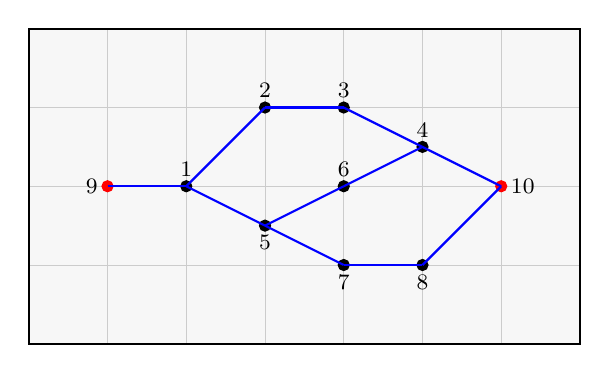
\begin{tikzpicture}% [scale=0.8] 
  \draw[step=1cm, very thin, gray!40] (0,0) grid (7,4);
  \draw[black, thick] (0,0) rectangle (7,4);
  \filldraw [red] (1,2) circle (2pt);
  \filldraw [red] (6,2) circle (2pt);
  \filldraw [black] (2,2) circle (2pt);
  \filldraw [black] (3,1.5) circle (2pt);
  \filldraw [black] (3,3) circle (2pt);
  \filldraw [black] (5,1) circle (2pt);
%  \filldraw [black] (5,2) circle (2pt);
  \filldraw [black] (4,2) circle (2pt);
  \filldraw [black] (5,2.5) circle (2pt);
  \filldraw [black] (4,3) circle (2pt);
  \filldraw [black] (4,1) circle (2pt);
%  \filldraw [black] (4,1) circle (2pt);
  \draw[thick,blue] (1,2) -- (2,2); 
  \draw[thick,blue] (3,1.5) -- (4,2);
  \draw[thick,blue] (3,3) -- (4,3);
  \draw[thick,blue] (4,3) -- (5,2.5);
  \draw[thick,blue] (2,2) -- (3,3);
  \draw[thick,blue] (2,2) -- (3,1.5);
  \draw[thick,blue] (5,2.5) -- (4,2);
%  \draw[thick,blue] (4,2) -- (4,1);
% \draw[thick,blue] (2,2) .. controls (3,1.5) .. (4,2);
  \draw[thick,blue] (3,1.5) -- (4,1);
  \draw[thick,blue] (4,1) -- (5,1);
  \draw[thick,blue] (5,2.5) -- (6,2);
%  \draw[thick,blue] (4,2) -- (5,2);
%  \draw[thick,blue] (5,2) -- (6,2);
  \draw[thick,blue] (5,1) -- (6,2);

  \node[anchor=east,font=\footnotesize] at (1,2) {9};
  \node[anchor=west,font=\footnotesize] at (6,2) {10};
  \node[anchor=south,font=\footnotesize] at (3,3) {2};
  \node[anchor=south,font=\footnotesize] at (4,3) {3};
  \node[anchor=north,font=\footnotesize] at (3,1.5) {5};
  \node[anchor=south,font=\footnotesize] at (5,2.5) {4};
  \node[anchor=south,font=\footnotesize] at (2,2) {1};
  \node[anchor=south,font=\footnotesize] at (4,2) {6};
  %\node[anchor=north,font=\small] at (3,1) {7};
  \node[anchor=north,font=\footnotesize] at (5,1) {8};
  \node[anchor=north,font=\footnotesize] at (4,1) {7};

  \begin{pgfonlayer}{background}
    \filldraw [line width=4mm,black!3]
      (0.2,0.2)  rectangle (6.8,3.8);
  \end{pgfonlayer}
\end{tikzpicture}}%


\begin{figure}[H]
  \begin{center}
  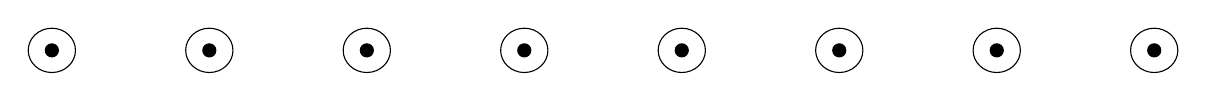
\begin{tikzpicture}[every node/.style={draw}] 
\centering
\node (l1) at (2,0) [circle,fill=black,scale=0.5] {};
\node (l2) at (4,0) [circle,fill=black,scale=0.5] {};
\node (l3) at (6,0) [circle,fill=black,scale=0.5] {};
\node (l4) at (8,0) [circle,fill=black,scale=0.5] {};
\node (l5) at (10,0) [circle,fill=black,scale=0.5] {};
\node (l6) at (12,0) [circle,fill=black,scale=0.5] {};
\node (l7) at (14,0) [circle,fill=black,scale=0.5] {};
\node (l8) at (16,0) [circle,fill=black,scale=0.5] {};

\draw let \p1=(l1), \p2=(l1), \n1={atan2(\y2-\y1,\x2-\x1)}, \n2={veclen(\y2-\y1,\x2-\x1)}
  in ($ (l1)!0.5!(l1) $) ellipse [x radius=\n2/2+8pt, y radius=0.3cm,rotate=0-\n1];
\draw let \p1=(l2), \p2=(l2), \n1={atan2(\y2-\y1,\x2-\x1)}, \n2={veclen(\y2-\y1,\x2-\x1)}
  in ($ (l2)!0.5!(l2) $) ellipse [x radius=\n2/2+8pt, y radius=0.3cm,rotate=0-\n1];
\draw let \p1=(l3), \p2=(l3), \n1={atan2(\y2-\y1,\x2-\x1)}, \n2={veclen(\y2-\y1,\x2-\x1)}
  in ($ (l3)!0.5!(l3) $) ellipse [x radius=\n2/2+8pt, y radius=0.3cm,rotate=0-\n1];
\draw let \p1=(l4), \p2=(l4), \n1={atan2(\y2-\y1,\x2-\x1)}, \n2={veclen(\y2-\y1,\x2-\x1)}
  in ($ (l4)!0.5!(l4) $) ellipse [x radius=\n2/2+8pt, y radius=0.3cm,rotate=0-\n1];
\draw let \p1=(l5), \p2=(l5), \n1={atan2(\y2-\y1,\x2-\x1)}, \n2={veclen(\y2-\y1,\x2-\x1)}
  in ($ (l5)!0.5!(l5) $) ellipse [x radius=\n2/2+8pt, y radius=0.3cm,rotate=0-\n1];
\draw let \p1=(l6), \p2=(l6), \n1={atan2(\y2-\y1,\x2-\x1)}, \n2={veclen(\y2-\y1,\x2-\x1)}
  in ($ (l6)!0.5!(l6) $) ellipse [x radius=\n2/2+8pt, y radius=0.3cm,rotate=0-\n1];
\draw let \p1=(l7), \p2=(l7), \n1={atan2(\y2-\y1,\x2-\x1)}, \n2={veclen(\y2-\y1,\x2-\x1)}
  in ($ (l7)!0.5!(l7) $) ellipse [x radius=\n2/2+8pt, y radius=0.3cm,rotate=0-\n1];
\draw let \p1=(l8), \p2=(l8), \n1={atan2(\y2-\y1,\x2-\x1)}, \n2={veclen(\y2-\y1,\x2-\x1)}
  in ($ (l8)!0.5!(l8) $) ellipse [x radius=\n2/2+8pt, y radius=0.3cm,rotate=0-\n1];
\end{tikzpicture}
\end{center}
  \vskip-0.2cm
  \caption{
 Single non-crossing partition
of $[1] \times [d]$ with $d=8$.} 
\label{f2-1}
\end{figure}

\vskip-0.4cm

\noindent


\begin{figure}[H]
  \begin{center}
\hskip-0.3cm
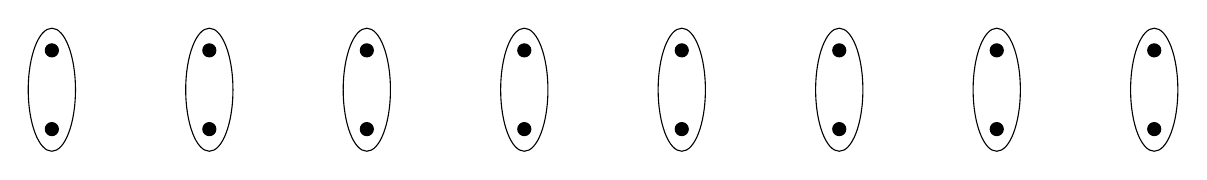
\begin{tikzpicture}[every node/.style={draw}] 
\centering
\node (l1) at (2,0) [circle,fill=black,scale=0.5] {};] {};
\node (l2) at (4,0) [circle,fill=black,scale=0.5] {};] {};
\node (l3) at (6,0) [circle,fill=black,scale=0.5] {};] {};
\node (l4) at (8,0) [circle,fill=black,scale=0.5] {};] {};
\node (l5) at (10,0) [circle,fill=black,scale=0.5] {};] {};
\node (l6) at (12,0) [circle,fill=black,scale=0.5] {};] {};
\node (l7) at (14,0) [circle,fill=black,scale=0.5] {};] {};
\node (l8) at (16,0) [circle,fill=black,scale=0.5] {};] {};

\node (m1) at (2,1) [circle,fill=black,scale=0.5] {};] {};
\node (m2) at (4,1) [circle,fill=black,scale=0.5] {};] {};
\node (m3) at (6,1) [circle,fill=black,scale=0.5] {};] {};
\node (m4) at (8,1) [circle,fill=black,scale=0.5] {};] {};
\node (m5) at (10,1) [circle,fill=black,scale=0.5] {};] {};
\node (m6) at (12,1) [circle,fill=black,scale=0.5] {};] {};
\node (m7) at (14,1) [circle,fill=black,scale=0.5] {};] {};
\node (m8) at (16,1) [circle,fill=black,scale=0.5] {};] {};

\draw let \p1=(l1), \p2=(m1), \n1={atan2(\y2-\y1,\x2-\x1)}, \n2={veclen(\y2-\y1,\x2-\x1)}
  in ($ (l1)!0.5!(m1) $) ellipse [x radius=\n2/2+8pt, y radius=0.3cm,rotate=0-\n1];
\draw let \p1=(l2), \p2=(m2), \n1={atan2(\y2-\y1,\x2-\x1)}, \n2={veclen(\y2-\y1,\x2-\x1)}
  in ($ (l2)!0.5!(m2) $) ellipse [x radius=\n2/2+8pt, y radius=0.3cm,rotate=0-\n1];
\draw let \p1=(l3), \p2=(m3), \n1={atan2(\y2-\y1,\x2-\x1)}, \n2={veclen(\y2-\y1,\x2-\x1)}
  in ($ (l3)!0.5!(m3) $) ellipse [x radius=\n2/2+8pt, y radius=0.3cm,rotate=0-\n1];
\draw let \p1=(l4), \p2=(m4), \n1={atan2(\y2-\y1,\x2-\x1)}, \n2={veclen(\y2-\y1,\x2-\x1)}
  in ($ (l4)!0.5!(m4) $) ellipse [x radius=\n2/2+8pt, y radius=0.3cm,rotate=0-\n1];
\draw let \p1=(l5), \p2=(m5), \n1={atan2(\y2-\y1,\x2-\x1)}, \n2={veclen(\y2-\y1,\x2-\x1)}
  in ($ (l5)!0.5!(m5) $) ellipse [x radius=\n2/2+8pt, y radius=0.3cm,rotate=0-\n1];
\draw let \p1=(l6), \p2=(m6), \n1={atan2(\y2-\y1,\x2-\x1)}, \n2={veclen(\y2-\y1,\x2-\x1)}
  in ($ (l6)!0.5!(m6) $) ellipse [x radius=\n2/2+8pt, y radius=0.3cm,rotate=0-\n1];
\draw let \p1=(l7), \p2=(m7), \n1={atan2(\y2-\y1,\x2-\x1)}, \n2={veclen(\y2-\y1,\x2-\x1)} in ($ (l7)!0.5!(m7) $) ellipse [x radius=\n2/2+8pt, y radius=0.3cm,rotate=0-\n1];
% \draw let \p1=(l8), \p2=(m7), \n1={atan2(\y2-\y1,\x2-\x1)}, \n2={veclen(\y2-\y1,\x2-\x1)}  in ($ (l8)!0.5!(m7) $) ellipse [x radius=\n2/2+8pt, y radius=0.3cm,rotate=0-\n1];
\draw let \p1=(l8), \p2=(m8), \n1={atan2(\y2-\y1,\x2-\x1)}, \n2={veclen(\y2-\y1,\x2-\x1)} in ($ (l8)!0.5!(m8) $) ellipse [x radius=\n2/2+8pt, y radius=0.3cm,rotate=0-\n1];
\end{tikzpicture}
\end{center}
  \vskip-0.2cm
  \caption{
 Non-crossing partition of $2 \times d$ with $d=8$.} 
% \label{f3-1-4}
\end{figure}

\begin{figure}[H]
  \begin{center}
\hskip-0.3cm
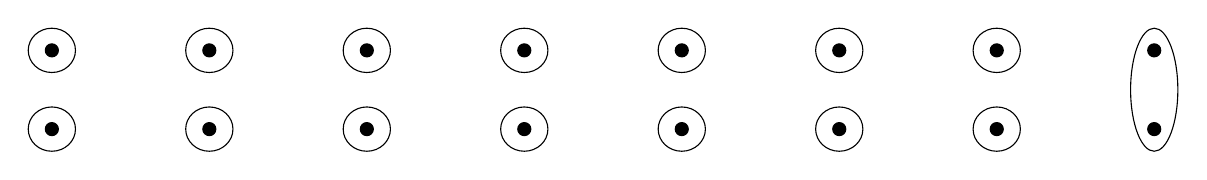
\begin{tikzpicture}[every node/.style={draw}] 
\centering
\node (l1) at (2,0) [circle,fill=black,scale=0.5] {};] {};
\node (l2) at (4,0) [circle,fill=black,scale=0.5] {};] {};
\node (l3) at (6,0) [circle,fill=black,scale=0.5] {};] {};
\node (l4) at (8,0) [circle,fill=black,scale=0.5] {};] {};
\node (l5) at (10,0) [circle,fill=black,scale=0.5] {};] {};
\node (l6) at (12,0) [circle,fill=black,scale=0.5] {};] {};
\node (l7) at (14,0) [circle,fill=black,scale=0.5] {};] {};
\node (l8) at (16,0) [circle,fill=black,scale=0.5] {};] {};

\node (m1) at (2,1) [circle,fill=black,scale=0.5] {};] {};
\node (m2) at (4,1) [circle,fill=black,scale=0.5] {};] {};
\node (m3) at (6,1) [circle,fill=black,scale=0.5] {};] {};
\node (m4) at (8,1) [circle,fill=black,scale=0.5] {};] {};
\node (m5) at (10,1) [circle,fill=black,scale=0.5] {};] {};
\node (m6) at (12,1) [circle,fill=black,scale=0.5] {};] {};
\node (m7) at (14,1) [circle,fill=black,scale=0.5] {};] {};
\node (m8) at (16,1) [circle,fill=black,scale=0.5] {};] {};

\draw let \p1=(l1), \p2=(l1), \n1={atan2(\y2-\y1,\x2-\x1)}, \n2={veclen(\y2-\y1,\x2-\x1)}
  in ($ (l1)!0.5!(l1) $) ellipse [x radius=\n2/2+8pt, y radius=0.3cm,rotate=0-\n1];
\draw let \p1=(m1), \p2=(m1), \n1={atan2(\y2-\y1,\x2-\x1)}, \n2={veclen(\y2-\y1,\x2-\x1)}
  in ($ (m1)!0.5!(m1) $) ellipse [x radius=\n2/2+8pt, y radius=0.3cm,rotate=0-\n1];
\draw let \p1=(l2), \p2=(l2), \n1={atan2(\y2-\y1,\x2-\x1)}, \n2={veclen(\y2-\y1,\x2-\x1)}
  in ($ (l2)!0.5!(l2) $) ellipse [x radius=\n2/2+8pt, y radius=0.3cm,rotate=0-\n1];
\draw let \p1=(m2), \p2=(m2), \n1={atan2(\y2-\y1,\x2-\x1)}, \n2={veclen(\y2-\y1,\x2-\x1)}
  in ($ (m2)!0.5!(m2) $) ellipse [x radius=\n2/2+8pt, y radius=0.3cm,rotate=0-\n1];
\draw let \p1=(l3), \p2=(l3), \n1={atan2(\y2-\y1,\x2-\x1)}, \n2={veclen(\y2-\y1,\x2-\x1)}
  in ($ (l3)!0.5!(l3) $) ellipse [x radius=\n2/2+8pt, y radius=0.3cm,rotate=0-\n1];
\draw let \p1=(m3), \p2=(m3), \n1={atan2(\y2-\y1,\x2-\x1)}, \n2={veclen(\y2-\y1,\x2-\x1)}
  in ($ (m3)!0.5!(m3) $) ellipse [x radius=\n2/2+8pt, y radius=0.3cm,rotate=0-\n1];
\draw let \p1=(l4), \p2=(l4), \n1={atan2(\y2-\y1,\x2-\x1)}, \n2={veclen(\y2-\y1,\x2-\x1)}
  in ($ (l4)!0.5!(l4) $) ellipse [x radius=\n2/2+8pt, y radius=0.3cm,rotate=0-\n1];
\draw let \p1=(m4), \p2=(m4), \n1={atan2(\y2-\y1,\x2-\x1)}, \n2={veclen(\y2-\y1,\x2-\x1)}
  in ($ (m4)!0.5!(m4) $) ellipse [x radius=\n2/2+8pt, y radius=0.3cm,rotate=0-\n1];
\draw let \p1=(l5), \p2=(l5), \n1={atan2(\y2-\y1,\x2-\x1)}, \n2={veclen(\y2-\y1,\x2-\x1)}
  in ($ (l5)!0.5!(l5) $) ellipse [x radius=\n2/2+8pt, y radius=0.3cm,rotate=0-\n1];
\draw let \p1=(m5), \p2=(m5), \n1={atan2(\y2-\y1,\x2-\x1)}, \n2={veclen(\y2-\y1,\x2-\x1)}
  in ($ (m5)!0.5!(m5) $) ellipse [x radius=\n2/2+8pt, y radius=0.3cm,rotate=0-\n1];
\draw let \p1=(l6), \p2=(l6), \n1={atan2(\y2-\y1,\x2-\x1)}, \n2={veclen(\y2-\y1,\x2-\x1)}
  in ($ (l6)!0.5!(l6) $) ellipse [x radius=\n2/2+8pt, y radius=0.3cm,rotate=0-\n1];
\draw let \p1=(m6), \p2=(m6), \n1={atan2(\y2-\y1,\x2-\x1)}, \n2={veclen(\y2-\y1,\x2-\x1)}
  in ($ (m6)!0.5!(m6) $) ellipse [x radius=\n2/2+8pt, y radius=0.3cm,rotate=0-\n1];
  \draw let \p1=(l7), \p2=(l7), \n1={atan2(\y2-\y1,\x2-\x1)}, \n2={veclen(\y2-\y1,\x2-\x1)} in ($ (l7)!0.5!(l7) $) ellipse [x radius=\n2/2+8pt, y radius=0.3cm,rotate=0-\n1];
  \draw let \p1=(m7), \p2=(m7), \n1={atan2(\y2-\y1,\x2-\x1)}, \n2={veclen(\y2-\y1,\x2-\x1)} in ($ (m7)!0.5!(m7) $) ellipse [x radius=\n2/2+8pt, y radius=0.3cm,rotate=0-\n1];
\draw let \p1=(l8), \p2=(m8), \n1={atan2(\y2-\y1,\x2-\x1)}, \n2={veclen(\y2-\y1,\x2-\x1)} in ($ (l8)!0.5!(m8) $) ellipse [x radius=\n2/2+8pt, y radius=0.3cm,rotate=0-\n1];
% \draw let \p1=(m8), \p2=(m8), \n1={atan2(\y2-\y1,\x2-\x1)}, \n2={veclen(\y2-\y1,\x2-\x1)} in ($ (m8)!0.5!(m8) $) ellipse [x radius=\n2/2+8pt, y radius=0.3cm,rotate=0-\n1];
\end{tikzpicture}
\end{center}
  \vskip-0.2cm
  \caption{
 Non-crossing partition
 of $2 \times d$ with $d=8$.} 
% \label{f3-1-3}
\end{figure}

\vskip-0.4cm

\begin{figure}[H]
  \begin{center}
\hskip-0.3cm
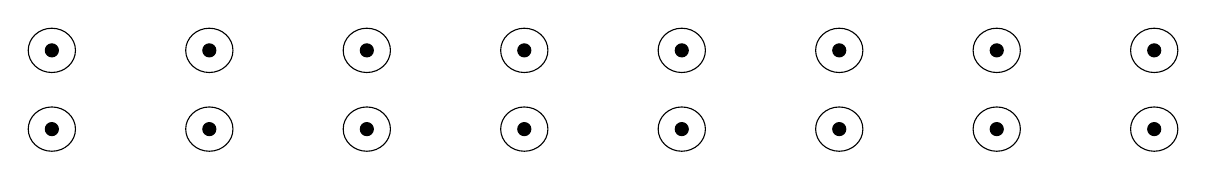
\begin{tikzpicture}[every node/.style={draw}] 
\centering
\node (l1) at (2,0) [circle,fill=black,scale=0.5] {};] {};
\node (l2) at (4,0) [circle,fill=black,scale=0.5] {};] {};
\node (l3) at (6,0) [circle,fill=black,scale=0.5] {};] {};
\node (l4) at (8,0) [circle,fill=black,scale=0.5] {};] {};
\node (l5) at (10,0) [circle,fill=black,scale=0.5] {};] {};
\node (l6) at (12,0) [circle,fill=black,scale=0.5] {};] {};
\node (l7) at (14,0) [circle,fill=black,scale=0.5] {};] {};
\node (l8) at (16,0) [circle,fill=black,scale=0.5] {};] {};

\node (m1) at (2,1) [circle,fill=black,scale=0.5] {};] {};
\node (m2) at (4,1) [circle,fill=black,scale=0.5] {};] {};
\node (m3) at (6,1) [circle,fill=black,scale=0.5] {};] {};
\node (m4) at (8,1) [circle,fill=black,scale=0.5] {};] {};
\node (m5) at (10,1) [circle,fill=black,scale=0.5] {};] {};
\node (m6) at (12,1) [circle,fill=black,scale=0.5] {};] {};
\node (m7) at (14,1) [circle,fill=black,scale=0.5] {};] {};
\node (m8) at (16,1) [circle,fill=black,scale=0.5] {};] {};

\draw let \p1=(l1), \p2=(l1), \n1={atan2(\y2-\y1,\x2-\x1)}, \n2={veclen(\y2-\y1,\x2-\x1)}
  in ($ (l1)!0.5!(l1) $) ellipse [x radius=\n2/2+8pt, y radius=0.3cm,rotate=0-\n1];
\draw let \p1=(m1), \p2=(m1), \n1={atan2(\y2-\y1,\x2-\x1)}, \n2={veclen(\y2-\y1,\x2-\x1)}
  in ($ (m1)!0.5!(m1) $) ellipse [x radius=\n2/2+8pt, y radius=0.3cm,rotate=0-\n1];
\draw let \p1=(l2), \p2=(l2), \n1={atan2(\y2-\y1,\x2-\x1)}, \n2={veclen(\y2-\y1,\x2-\x1)}
  in ($ (l2)!0.5!(l2) $) ellipse [x radius=\n2/2+8pt, y radius=0.3cm,rotate=0-\n1];
\draw let \p1=(m2), \p2=(m2), \n1={atan2(\y2-\y1,\x2-\x1)}, \n2={veclen(\y2-\y1,\x2-\x1)}
  in ($ (m2)!0.5!(m2) $) ellipse [x radius=\n2/2+8pt, y radius=0.3cm,rotate=0-\n1];
\draw let \p1=(l3), \p2=(l3), \n1={atan2(\y2-\y1,\x2-\x1)}, \n2={veclen(\y2-\y1,\x2-\x1)}
  in ($ (l3)!0.5!(l3) $) ellipse [x radius=\n2/2+8pt, y radius=0.3cm,rotate=0-\n1];
\draw let \p1=(m3), \p2=(m3), \n1={atan2(\y2-\y1,\x2-\x1)}, \n2={veclen(\y2-\y1,\x2-\x1)}
  in ($ (m3)!0.5!(m3) $) ellipse [x radius=\n2/2+8pt, y radius=0.3cm,rotate=0-\n1];
\draw let \p1=(l4), \p2=(l4), \n1={atan2(\y2-\y1,\x2-\x1)}, \n2={veclen(\y2-\y1,\x2-\x1)}
  in ($ (l4)!0.5!(l4) $) ellipse [x radius=\n2/2+8pt, y radius=0.3cm,rotate=0-\n1];
\draw let \p1=(m4), \p2=(m4), \n1={atan2(\y2-\y1,\x2-\x1)}, \n2={veclen(\y2-\y1,\x2-\x1)}
  in ($ (m4)!0.5!(m4) $) ellipse [x radius=\n2/2+8pt, y radius=0.3cm,rotate=0-\n1];
\draw let \p1=(l5), \p2=(l5), \n1={atan2(\y2-\y1,\x2-\x1)}, \n2={veclen(\y2-\y1,\x2-\x1)}
  in ($ (l5)!0.5!(l5) $) ellipse [x radius=\n2/2+8pt, y radius=0.3cm,rotate=0-\n1];
\draw let \p1=(m5), \p2=(m5), \n1={atan2(\y2-\y1,\x2-\x1)}, \n2={veclen(\y2-\y1,\x2-\x1)}
  in ($ (m5)!0.5!(m5) $) ellipse [x radius=\n2/2+8pt, y radius=0.3cm,rotate=0-\n1];
\draw let \p1=(l6), \p2=(l6), \n1={atan2(\y2-\y1,\x2-\x1)}, \n2={veclen(\y2-\y1,\x2-\x1)}
  in ($ (l6)!0.5!(l6) $) ellipse [x radius=\n2/2+8pt, y radius=0.3cm,rotate=0-\n1];
\draw let \p1=(m6), \p2=(m6), \n1={atan2(\y2-\y1,\x2-\x1)}, \n2={veclen(\y2-\y1,\x2-\x1)}
  in ($ (m6)!0.5!(m6) $) ellipse [x radius=\n2/2+8pt, y radius=0.3cm,rotate=0-\n1];
  \draw let \p1=(l7), \p2=(l7), \n1={atan2(\y2-\y1,\x2-\x1)}, \n2={veclen(\y2-\y1,\x2-\x1)} in ($ (l7)!0.5!(l7) $) ellipse [x radius=\n2/2+8pt, y radius=0.3cm,rotate=0-\n1];
  \draw let \p1=(m7), \p2=(m7), \n1={atan2(\y2-\y1,\x2-\x1)}, \n2={veclen(\y2-\y1,\x2-\x1)} in ($ (m7)!0.5!(m7) $) ellipse [x radius=\n2/2+8pt, y radius=0.3cm,rotate=0-\n1];
\draw let \p1=(l8), \p2=(l8), \n1={atan2(\y2-\y1,\x2-\x1)}, \n2={veclen(\y2-\y1,\x2-\x1)} in ($ (l8)!0.5!(l8) $) ellipse [x radius=\n2/2+8pt, y radius=0.3cm,rotate=0-\n1];
\draw let \p1=(m8), \p2=(m8), \n1={atan2(\y2-\y1,\x2-\x1)}, \n2={veclen(\y2-\y1,\x2-\x1)} in ($ (m8)!0.5!(m8) $) ellipse [x radius=\n2/2+8pt, y radius=0.3cm,rotate=0-\n1];
\end{tikzpicture}
\end{center}
  \vskip-0.2cm
  \caption{
 Non-crossing partition
 of $2 \times d$ with $d=8$.} 
% \label{f3-1-2}
\end{figure}

\vskip-0.4cm


\begin{figure}[H]
\centering 
\hskip-0.3cm
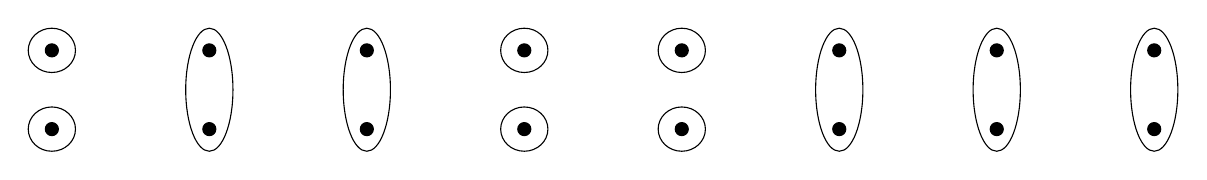
\begin{tikzpicture}[every node/.style={draw}] 
\centering
\node (l1) at (2,0) [circle,fill=black,scale=0.5] {};] {};
\node (l2) at (4,0) [circle,fill=black,scale=0.5] {};] {};
\node (l3) at (6,0) [circle,fill=black,scale=0.5] {};] {};
\node (l4) at (8,0) [circle,fill=black,scale=0.5] {};] {};
\node (l5) at (10,0) [circle,fill=black,scale=0.5] {};] {};
\node (l6) at (12,0) [circle,fill=black,scale=0.5] {};] {};
\node (l7) at (14,0) [circle,fill=black,scale=0.5] {};] {};
\node (l8) at (16,0) [circle,fill=black,scale=0.5] {};] {};

\node (m1) at (2,1) [circle,fill=black,scale=0.5] {};] {};
\node (m2) at (4,1) [circle,fill=black,scale=0.5] {};] {};
\node (m3) at (6,1) [circle,fill=black,scale=0.5] {};] {};
\node (m4) at (8,1) [circle,fill=black,scale=0.5] {};] {};
\node (m5) at (10,1) [circle,fill=black,scale=0.5] {};] {};
\node (m6) at (12,1) [circle,fill=black,scale=0.5] {};] {};
\node (m7) at (14,1) [circle,fill=black,scale=0.5] {};] {};
\node (m8) at (16,1) [circle,fill=black,scale=0.5] {};] {};

\draw let \p1=(l1), \p2=(l1), \n1={atan2(\y2-\y1,\x2-\x1)}, \n2={veclen(\y2-\y1,\x2-\x1)}
  in ($ (l1)!0.5!(l1) $) ellipse [x radius=\n2/2+8pt, y radius=0.3cm,rotate=0-\n1];
\draw let \p1=(m1), \p2=(m1), \n1={atan2(\y2-\y1,\x2-\x1)}, \n2={veclen(\y2-\y1,\x2-\x1)}
  in ($ (m1)!0.5!(m1) $) ellipse [x radius=\n2/2+8pt, y radius=0.3cm,rotate=0-\n1];
\draw let \p1=(l2), \p2=(m2), \n1={atan2(\y2-\y1,\x2-\x1)}, \n2={veclen(\y2-\y1,\x2-\x1)}
  in ($ (l2)!0.5!(m2) $) ellipse [x radius=\n2/2+8pt, y radius=0.3cm,rotate=0-\n1];
\draw let \p1=(l3), \p2=(m3), \n1={atan2(\y2-\y1,\x2-\x1)}, \n2={veclen(\y2-\y1,\x2-\x1)}
  in ($ (l3)!0.5!(m3) $) ellipse [x radius=\n2/2+8pt, y radius=0.3cm,rotate=0-\n1];
\draw let \p1=(l4), \p2=(l4), \n1={atan2(\y2-\y1,\x2-\x1)}, \n2={veclen(\y2-\y1,\x2-\x1)}
  in ($ (l4)!0.5!(l4) $) ellipse [x radius=\n2/2+8pt, y radius=0.3cm,rotate=0-\n1];
\draw let \p1=(m4), \p2=(m4), \n1={atan2(\y2-\y1,\x2-\x1)}, \n2={veclen(\y2-\y1,\x2-\x1)}
  in ($ (m4)!0.5!(m4) $) ellipse [x radius=\n2/2+8pt, y radius=0.3cm,rotate=0-\n1];
\draw let \p1=(l5), \p2=(l5), \n1={atan2(\y2-\y1,\x2-\x1)}, \n2={veclen(\y2-\y1,\x2-\x1)}
  in ($ (l5)!0.5!(l5) $) ellipse [x radius=\n2/2+8pt, y radius=0.3cm,rotate=0-\n1];
\draw let \p1=(m5), \p2=(m5), \n1={atan2(\y2-\y1,\x2-\x1)}, \n2={veclen(\y2-\y1,\x2-\x1)}
  in ($ (m5)!0.5!(m5) $) ellipse [x radius=\n2/2+8pt, y radius=0.3cm,rotate=0-\n1];
\draw let \p1=(l6), \p2=(m6), \n1={atan2(\y2-\y1,\x2-\x1)}, \n2={veclen(\y2-\y1,\x2-\x1)}
  in ($ (l6)!0.5!(m6) $) ellipse [x radius=\n2/2+8pt, y radius=0.3cm,rotate=0-\n1];
\draw let \p1=(l7), \p2=(m7), \n1={atan2(\y2-\y1,\x2-\x1)}, \n2={veclen(\y2-\y1,\x2-\x1)} in ($ (l7)!0.5!(m7) $) ellipse [x radius=\n2/2+8pt, y radius=0.3cm,rotate=0-\n1];
% \draw let \p1=(l8), \p2=(m7), \n1={atan2(\y2-\y1,\x2-\x1)}, \n2={veclen(\y2-\y1,\x2-\x1)}  in ($ (l8)!0.5!(m7) $) ellipse [x radius=\n2/2+8pt, y radius=0.3cm,rotate=0-\n1];
\draw let \p1=(l8), \p2=(m8), \n1={atan2(\y2-\y1,\x2-\x1)}, \n2={veclen(\y2-\y1,\x2-\x1)} in ($ (l8)!0.5!(m8) $) ellipse [x radius=\n2/2+8pt, y radius=0.3cm,rotate=0-\n1];
% \draw let \p1=(l7), \p2=(m8), \n1={atan2(\y2-\y1,\x2-\x1)}, \n2={veclen(\y2-\y1,\x2-\x1)} in ($ (l7)!0.5!(m8) $) ellipse [x radius=\n2/2+8pt, y radius=0.3cm,rotate=0-\n1];
\end{tikzpicture}
\vskip-0.2cm
\caption{
 Example of a non-crossing partition
of $2 \times d$ with $d=8$.} 
\label{f3-1-1}
\end{figure}


\def\cprime{$'$} \def\polhk#1{\setbox0=\hbox{#1}{\ooalign{\hidewidth
  \lower1.5ex\hbox{`}\hidewidth\crcr\unhbox0}}}
  \def\polhk#1{\setbox0=\hbox{#1}{\ooalign{\hidewidth
  \lower1.5ex\hbox{`}\hidewidth\crcr\unhbox0}}} \def\cprime{$'$}
\begin{thebibliography}{KGKP21}

\bibitem[BCJ23]{bhattacharya23}
B.~Bhattacharya, A.~Chatterjee, and S.~Janson.
\newblock Fluctuations of subgraph counts in graphon based random graphs.
\newblock {\em Combin. Probab. Comput.}, 32(3):428--464, 2023.

\bibitem[BHJ92]{BarbourHolstJanson}
A.D. Barbour, L.~Holst, and S.~Janson.
\newblock {\em Poisson approximation}, volume~2 of {\em Oxford Studies in
  Probability}.
\newblock The Clarendon Press, Oxford University Press, New York, 1992.

\bibitem[CGR16]{coulson16}
M.~Coulson, R.~E. Gaunt, and G.~Reinert.
\newblock Poisson approximation of subgraph counts in stochastic block models
  and a graphon model.
\newblock {\em ESAIM Probab. Stat.}, 20:131--142, 2016.

\bibitem[Che75]{chen1975}
L.H.Y. Chen.
\newblock Poisson approximation for dependent trials.
\newblock {\em Ann. Probab.}, 3(3):534--545, 1975.

\bibitem[DE13]{doring}
H.~D{\"{o}}ring and P.~Eichelsbacher.
\newblock Moderate deviations via cumulants.
\newblock {\em J. Theoret. Probab.}, 26:360--385, 2013.

\bibitem[DF14]{DevroyeFraiman14}
L.~Devroye and N.~Fraiman.
\newblock Connectivity of inhomogeneous random graphs.
\newblock {\em Random Structures Algorithms}, 45(3):408--420, 2014.

\bibitem[DJS22]{doering}
H.~D{\"o}ring, S.~Jansen, and K.~Schubert.
\newblock The method of cumulants for the normal approximation.
\newblock {\em Probab. Surv.}, 19:185--270, 2022.

\bibitem[Dro97]{drory1997}
A.~Drory.
\newblock Exact solution of a one-dimensional continuum percolation model.
\newblock {\em Phys. Rev. E (3)}, 55(4):3878--3885, 1997.

\bibitem[GK19]{AGK19}
R.~Arratia~L. Goldstein and F.~Kochman.
\newblock Size bias for one and all.
\newblock {\em Probab. Surv.}, 16:161, 2019.

\bibitem[GT18]{thale18}
J.~Grote and C.~Th{\"a}le.
\newblock Gaussian polytopes: a cumulant-based approach.
\newblock {\em J. Complexity}, 47:1--41, 2018.

\bibitem[HHO25]{heerten}
N.~Heerten, C.~Hirsch, and M.~Otto.
\newblock Moderate deviations for weight-dependent random connection models.
\newblock {\em J. Appl. Probab.}, pages 1--23, 2025.

\bibitem[HP{\v{C}}21]{hladky21}
J.~Hladk{\'y}, C.~Pelekis, and M.~{\v{C}}ileikis.
\newblock A limit theorem for small cliques in inhomogeneous random graphs.
\newblock {\em J. Graph Theory}, 97:578--599, 2021.

\bibitem[Jan88]{Janson1988}
S.~Janson.
\newblock Normal convergence by higher semiinvariants with applications to sums
  of dependent random variables and random graphs.
\newblock {\em Ann. Probab.}, 16(1):305--312, 1988.

\bibitem[J{\L}R00]{JLR}
S.~Janson, T.~{\L}uczak, and A.~Ruci{\'n}ski.
\newblock {\em Random graphs}.
\newblock Wiley-Interscience Series in Discrete Mathematics and Optimization.
  Wiley-Interscience, New York, 2000.

\bibitem[KGKP21]{giles-privault}
A.P. Kartun-Giles, K.~Koufos, and N.~Privault.
\newblock Connectivity of 1d random geometric graphs.
\newblock Preprint arXiv:2105.07731, 2021.

\bibitem[Kho08]{khorunzhiy}
O.~Khorunzhiy.
\newblock On connected diagrams and cumulants of {E}rd{\Horig{o}}s-{R}\'enyi
  matrix models.
\newblock {\em Comm. Math. Phys.}, 282:209--238, 2008.

\bibitem[LP24]{LiuPrivault}
Q.~Liu and N.~Privault.
\newblock Normal approximation of subgraph counts in the random-connection
  model.
\newblock {\em Bernoulli}, 30:3224--3250, 2024.

\bibitem[LP25a]{LiuPrivault25}
Q.~Liu and N.~Privault.
\newblock Gaussian fluctuations of generalized {$U$}-statistics and subgraph
  counting in the binomial random-connection model.
\newblock Preprint arXiv:2505.12338, 33 pages, 2025.

\bibitem[LP25b]{LiuPri23b}
Q.~Liu and N.~Privault.
\newblock Graph connectivity with fixed endpoints in the random-connection
  model.
\newblock {\em Probability in the Engineering and Informational Sciences},
  39(3):370--396, 2025.

\bibitem[LS59]{leonov}
V.P. Leonov and A.N. Shiryaev.
\newblock {On a method of calculation of semi-invariants.}
\newblock {\em Theory Probab. Appl.}, 4:319--329, 1959.

\bibitem[Luk55]{elukacs}
E.~Lukacs.
\newblock Applications of {F}a\`a di {B}runo's formula in mathematical
  statistics.
\newblock {\em Amer. Math. Monthly}, 62:340--348, 1955.

\bibitem[LX20]{LiuXia20}
Q.~Liu and A.~Xia.
\newblock On moderate deviations in {P}oisson approximation.
\newblock {\em J. Appl. Probab.}, 57(3):1005--1027, 2020.

\bibitem[Mal80]{malyshev1980}
V.A. Malyshev.
\newblock Cluster expansions in lattice models of statistical physics and the
  theory of quantum fields.
\newblock {\em Russian Mathematical Surveys}, 35(1):1--62, 1980.

\bibitem[McC87]{mccullagh}
P.~McCullagh.
\newblock {\em Tensor methods in statistics}.
\newblock Monographs on Statistics and Applied Probability. Chapman \& Hall,
  London, 1987.

\bibitem[MM91]{MalyshevMinlos91}
V.A. Malyshev and R.A. Minlos.
\newblock {\em Gibbs Random Fields}, volume~44 of {\em Mathematics and its
  Applications (Soviet Series)}.
\newblock Kluwer Academic Publishers Group, Dordrecht, 1991.

\bibitem[Pen18]{penrose18}
M.~Penrose.
\newblock Inhomogeneous random graphs, isolated vertices, and {P}oisson
  approximation.
\newblock {\em J. Appl. Probab.}, 55(1):112--136, 2018.

\bibitem[Pri24]{privaultkhops}
N.~Privault.
\newblock Asymptotic analysis of $k$-hop connectivity in the 1{D} unit disk
  random graph model.
\newblock {\em Methodol. Comput. Appl. Probab.}, 26(47), 2024.

\bibitem[PT11]{peccatitaqqu}
G.~Peccati and M.~Taqqu.
\newblock {\em Wiener Chaos: Moments, Cumulants and Diagrams: A survey with
  Computer Implementation}.
\newblock Bocconi \& Springer Series. Springer, 2011.

\bibitem[Ros11]{nross}
N.~Ross.
\newblock Fundamentals of {S}tein's method.
\newblock {\em Probab. Surv.}, 8:201--293, 2011.

\bibitem[Rot75]{rotabk}
G.-C. Rota, editor.
\newblock {\em Finite operator calculus}.
\newblock Academic Press, 1975.
\newblock With the collaboration of P. Doubilet, C. Greene, D. Kahaner, A.
  Odlyzko and R. Stanley.

\bibitem[RSS78]{rudzkis}
R.~Rudzkis, L.~Saulis, and V.A. Statulevi\v{c}ius.
\newblock A general lemma on probabilities of large deviations.
\newblock {\em Litovsk. Mat. Sb.}, 18(2):99--116, 217, 1978.

\bibitem[SS91]{saulis}
L.~Saulis and V.A. Statulevi\v{c}ius.
\newblock {\em Limit Theorems for Large Deviations}, volume~73 of {\em
  Mathematics and its Applications (Soviet Series)}.
\newblock Kluwer Academic Publishers Group, Dordrecht, 1991.

\bibitem[ST24]{schulte-thaele}
M.~Schulte and C.~Th{\"a}le.
\newblock Moderate deviations on {P}oisson chaos.
\newblock {\em Electron. J. Probab.}, 29:no. 146, 1--27, 2024.

\bibitem[Sta99]{stanley}
R.P. Stanley.
\newblock {\em Enumerative combinatorics. {V}ol. 2}, volume~62 of {\em
  Cambridge Studies in Advanced Mathematics}.
\newblock Cambridge University Press, Cambridge, 1999.

\bibitem[Zha22]{zhangzs}
Z.S. Zhang.
\newblock Berry-{E}sseen bounds for generalized {$U$}-statistics.
\newblock {\em Electron. J. Probab.}, 27:1--36, 2022.

\end{thebibliography}

On the other side,
when $p_m\ll m^{-1}$, we can show that 
for all $q=d+1,\dots,(d-1)n+1$, 
\begin{align*}
	\frac{m^d p_m^{d+1}}{m^q p_m^{\zeta(n,d,q)}}\gg 1.
\end{align*}

\noindent
  $(a)$ 
 When $m^{-1}\ll p_m$, 
%  using \eqref{convex1} and \eqref{convex2}, 
  for any $q\in \{d,\ldots,1+(d-1)n\}$ we have 
\begin{align*}
  \frac{m^{1+(d-1)n}p_m^{nd+1}}{m^qp_m^{\zeta (n,d,q)}}
  &= m^{1+(d-1)n-q}p_m^{nd+1-\zeta (n,d,q)}
  \\
  &= \left( mp_m^{\frac{nd+1-\zeta (n,d,q)}{nd+1-n-q}}\right)^{1+(d-1)n-q}
  \\
  &\gtrsim \left( mp_m^{d/(d-1)} \right)^{1+(d-1)n-q}
% \\ &=  \left( np_n^{\frac{e(G)}{d-1}}\right)^{1+(d-1)j-r}
  \\
  & \gg  1.
  % \frac{n^{jd-r}p_n^{je(G)-\zeta (n,d,r)}}{n^{jd-1-(d-1)j}p_n^{je(G)-je(G)}}\\
  % &=&\frac{n^{jd-r}p_n^{je(G)-\zeta (n,d,r)}}{n^{j-1}}\\
\end{align*}


\begin{figure}[H]
  \centering
   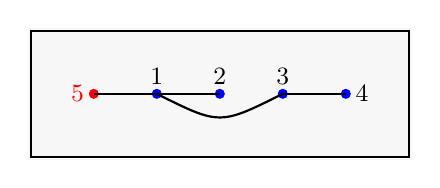
\begin{tikzpicture}[scale=0.8] 
\draw[black, thick] (0,0) rectangle (6,2);
\filldraw [red] (1,1) circle (2pt);
\foreach \i in {2,3,4,5}
{
\filldraw [blue] (\i,1) circle (2pt);
}
\draw[thick] (1,1) -- (3,1);
\draw[thick] (4,1) -- (5,1);
\draw[thick] (2,1) .. controls (3,0.5) .. (4,1);
\node[anchor=south,font=\small] at (2,1) {1};
\node[anchor=south,font=\small] at (3,1) {2};
\node[anchor=south,font=\small] at (4,1) {3};
\node[anchor=west,font=\small] at (5,1) {4};
\node[anchor=east,red,font=\small] at (1,1) {5};
  \begin{pgfonlayer}{background}
    \filldraw [line width=4mm,black!3]
      (0.2,0.2)  rectangle (5.8,1.8);
  \end{pgfonlayer}
  \end{tikzpicture}
   \caption{Connected graph $G$ on five vertices including one endpoint, with $r=4$ and $m=1$.}
   \label{fig:graph1}
   \end{figure}
   
 \vspace{-0.4cm}

 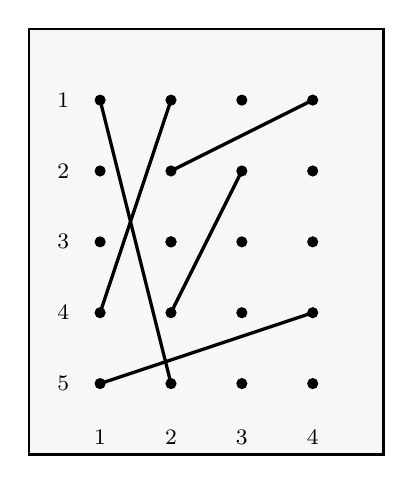
\begin{tikzpicture}[scale=0.9] 
  \draw[black, thick] (0,0) rectangle (5,6);
  
  \node[anchor=east,font=\footnotesize] at (0.7,5) {1};
  \node[anchor=east,font=\footnotesize] at (0.7,4) {2};
  \node[anchor=east,font=\footnotesize] at (0.7,3) {3};
  \node[anchor=east,font=\footnotesize] at (0.7,2) {4};
  \node[anchor=east,font=\footnotesize] at (0.7,1) {5};
  
  \node[anchor=south,font=\footnotesize] at (1,0) {1};
  \node[anchor=south,font=\footnotesize] at (2,0) {2};
  \node[anchor=south,font=\footnotesize] at (3,0) {3};
  \node[anchor=south,font=\footnotesize] at (4,0) {4};
  
  \filldraw [black] (1,1) circle (2pt);
  \filldraw [black] (2,1) circle (2pt);
  \filldraw [black] (3,1) circle (2pt);
  \filldraw [black] (4,1) circle (2pt);
  \filldraw [black] (1,2) circle (2pt);
  \filldraw [black] (2,2) circle (2pt);
  \filldraw [black] (3,2) circle (2pt);
  \filldraw [black] (4,2) circle (2pt);
  \filldraw [black] (1,3) circle (2pt);
  \filldraw [black] (2,3) circle (2pt);
  \filldraw [black] (3,3) circle (2pt);
  \filldraw [black] (4,3) circle (2pt);
  \filldraw [black] (2,3) circle (2pt);
  \filldraw [black] (1,4) circle (2pt);
  \filldraw [black] (2,4) circle (2pt);
  \filldraw [black] (3,4) circle (2pt);
  \filldraw [black] (4,4) circle (2pt);
  \filldraw [black] (1,5) circle (2pt);
  \filldraw [black] (2,5) circle (2pt);
  \filldraw [black] (3,5) circle (2pt);
  \filldraw [black] (4,5) circle (2pt);
  
  \draw[very thick] (1,2) -- (2,5);
  \draw[very thick] (1,1) -- (4,2);
  \draw[very thick] (1,5) -- (2,1);
  \draw[very thick] (2,2) -- (3,4);
  \draw[very thick] (2,4) -- (4,5);
 \begin{pgfonlayer}{background}
    \filldraw [line width=4mm,black!3]
      (0.2,0.2)  rectangle (4.8,5.8);
  \end{pgfonlayer}
  \end{tikzpicture}}%


Let now $[m_1] \times \cdots \times [m_d]$
 denote the collection of distinct $d$-fold indexes 
\begin{equation}
\nonumber % \label{indexset} 
    [m_1] \times \cdots \times [m_d]_{\ne}:=\{\beta =(\beta (1),\dots,\beta (d))\in
    [m_1] \times \cdots \times [m_d]
    \ : \
    \beta (i)\ne\beta (j),
     \ \leq i\ne j\leq d\},
\end{equation}
$d \geq 1$.

\begin{prop}
% \label{fsklf34}
  Let $k\geq 2$ and $t\in [(k-1)r,kr)$.
  The normalized $k$-hop count 
$\widebar{\sigma}_k^{(m)} (t)$ 
satisfies the Wasserstein and Kolmogorov bounds 
\begin{equation}
\label{fjkldsf-2} 
% d_K( \widebar{\sigma}_k (t) , {\cal N} ) :=
d_{K/W} \big( \widebar{\sigma}_k^{(m)} (t) , {\cal N} \big)
\leq \frac{C(k,r)}{\sqrt{\lambda}}
\end{equation} 
 for some constant $C(k,r)>0$, as $\lambda$ tends to infinity. 
\end{prop}
\begin{Proof}
 The kurtosis of $\sigma_k^{(m)}(t )$ satisfies 
\begin{eqnarray*} 
 \frac{\E_\lambda [ ( \sigma_k(t) -  \E_\lambda [ \sigma_k(t) ] )^4 ]}{( \Var_\lambda [ \sigma_k (t)] )^2} - 3
 & = & 
 \E_\lambda \big[ \big( \widebar{\sigma}_k^{(m)}(t) \big)^4 \big] - 3 
 \\
 & = & 
 \frac{c_{k,4}^{(m)} (kr-t;kr-t;kr-t;kr-t)}{( \Var_\lambda [ \sigma_k (t)] )^2} 
 \\
  & = & 
(B_4)^{k-2} O (m^{-1} ), 
\end{eqnarray*} 
 as $m$ tends to infinity. 
 The Kolmogorov distance bound in \eqref{fjkldsf-2} 
 then follows from the fourth moment theorem for $U$-statistics and sums of
 multiple stochastic integrals Corollary~4.10 in \cite{eichelsbacher}
 see also Theorem~3 in \cite{lachieze-rey}. 

 \medskip

 Regarding the Wasserstein distance bound,
 we can represent $\sigma_k^{(m)} (t)$ 
 as the $U$-statistics  
$$ 
 \sigma_k^{(m)} (t) 
 = 
 \sum_{((x_1,l_1),\ldots , ((x_{k-1},l_{k-1}) ) \in \omega^{k-1}
   \atop (x_i,l_i)\not=(x_j,l_j), 1\leq i\not= j \leq d}
 \tilde{f}_{\lambda ( kr -t) } (x_1/\lambda ,l_1;\ldots ; x_{k-1}/\lambda ,l_{k-1} )
$$
 of order $k-1$, where $\tilde{f}_t:( [0,r] \times \{1,\ldots , k-1\})^{k-1} \to \{0,1\}$,
 given by 
$$
\tilde{f}_t (x_1,l_1;\ldots , x_{k-1};l_{k-1})
:= \frac{1}{(k-1)!} \prod_{i=0}^{k-1} {\bf 1}_{\{(l_{i+1}-l_i)x_i<(l_{i+1}-l_i)x_{i+1} \}}, 
$$ 
 $((x_1,l_1),\ldots , (x_{k-1},l_{k-1}))\in ([0,r]\times \{1,\ldots , k-1\})^{k-1}$
 is the symmetrization in
 $k-1$ variables in $[0,r]\times \{1,\ldots , k-1\}$ of $f_t$. 
% , where $$ h(x,x',l,l') : = {\bf 1}_{\{x<x'\}} {\bf 1}_{\{l<l'\}}, \qquad x, x', l, l' \geq 0. $$
  Theorem~4.7 in \cite{reitzner} yields the bound 
  $$
  d_W\big(\widebar{\sigma}_k^{(m)}, {\cal N}\big) \leq
  \sum_{1\leq i \leq j < k}
  \frac{\sqrt{M_{i,j}}}{\Var_m [ \sigma_k(t)]}
 $$
 where   
 $M_{i,j}$ is defined in (14) therein satisfies
$$
 M_{1,1} \leq (k-1)^4 
 ( m r)^{4d-3}, \qquad  i,j=1. 
$$ 
 and
  $$
 M_{i,j} \leq {k-1 \choose i}^2 {k-1 \choose j}^2
 ( m r)^{4d-i-j}, \qquad  
 2\leq i \leq j < k. 
$$  
 Hence by \eqref{fjkdls45} and \eqref{dfjkvar} we have
\begin{eqnarray*} 
  \lefteqn{
    d_W\big(\widebar{\sigma}_k^{(m)}, {\cal N}\big)
  }
  \\
   & \leq & 
  \frac{1}{\Var_m [ \sigma_k(t)]}
  \left(
  (k-1)^2 ( m r)^{2(k-1)-3/2}
  +
  \sum_{2\leq i \leq j < k}
  {k-1 \choose i} {k-1 \choose j}
  ( m r)^{2(k-1)-i/2-j/2}
  \right)  
  \\
% & \lesssim &
  & \leq & 
  \frac{C(k)}{\sqrt{m r}} 
  +
  C(k,r) \sum_{2\leq i \leq j < k}
  ( m r)^{1-i/2-j/2}. 
\end{eqnarray*}
 The above conclusions can also be reached by 
 noting that $\widebar{\sigma}_k^{(m)}$ admits a Hoeffding decomposition
 and by applying Theorem~1.3 in \cite{doblerpeccati} for the Wasserstein
% distance, or Theorem~4.2 in \cite{PS4---revised}
 distance, or Theorem~6.3 in \cite{PS4} 
 for the Kolmogorov distance, which refine the central limit
 theorem of \cite{dejong1990}.
\end{Proof}

\subsubsection*{Normal approximation} % bounds}
The following result shows that
the normalized $k$-hop count
$$
\widebar{\sigma}_k := \frac{\sigma_k - \E[\sigma_k]}{\sqrt{\Var_m [ \sigma_k]}}
$$
converges in distribution to the standard normal
distribution as $m$ tends to infinity. 

In addition, \eqref{stat}
shows that the Statulevi\v{c}ius condition,
see \S~1.3 of \cite{doering},
is satisfied with $\gamma := k-3$ and $\Delta := \sqrt{\lambda}$.
By \cite{rudzkis},
   Corollary~2.1 in \S~1.3 in \cite{saulis},
   see also Theorem~2.4 in \cite{doering}, this yields the Kolmogorov
   distance bound
   \begin{equation}
\nonumber % \label{fjkf} 
 d_K \big( \widebar{\sigma}_k^{(m)} (t) , {\cal N} \big) 
\leq \frac{C(k,r)}{\lambda^{1/(2 + 4(k-3))}}
\end{equation} 
   for $t\in [(k-1)r,kr)$, as $\lambda$ tends to infinity.
\begin{corollary}
\label{cjkfl0} 
% Let $f:[0,r]^d \to\real$ be a measurable function with $d\geq 2$, such that $f$ satisfies Assumption~\ref{assu1}. 
  For $m\ge 4d$, 
  the $n$-$th$ cumulant of the normalized $U$-statistics 
  $$
  \widebar{\sigma}_k (kr-\tau):=
  \frac{\sigma_k(kr - \tau )-\kappa_1(\sigma_k(kr - \tau ))}{\sqrt{
      \sigma_k(kr - \tau )
      )}}
    $$ 
 satisfies the bound 
$$ 
    \kappa_n ( \widebar{\sigma}_k (kr-\tau) )\leq
    \frac{(n!)^{d+1}}{\big(m \widetilde{C}(f,d)\big)^{n/2-1}},
$$
    $n\geq 3$, where $\widetilde{C}(f,d)>0$ depends only on
    $d \geq 2$.
    \end{corollary}
\begin{Proof}
 Combining the inequalities 
\begin{equation}
\nonumber % \label{fjklf11} 
    \frac{m!}{(m-2d+1)!}\ge(m-2d+2)^{2d-1}
     =\left(1-\frac{2d-2}m\right)^{2d-1}m^{2d-1}
     \ge
     \left(\frac{m}{2}\right)^{2d-1}, 
\end{equation}
 $m\ge 4d$, and % From the inequality $\sqrt{2\pi n}({n}/{e})^n<n!$, we have
\begin{equation} 
\nonumber % \label{djkld1111} 
  n^{n-1}<\frac{(n-1)!}{\sqrt{2\pi n}}e^n< e^nn!,
  \quad n\geq 1, 
\end{equation}
 with the bound \eqref{fjkldf} and the equivalence \eqref{fjkdls45} 
 for $n\ge3$, we have 
\begin{align}
      \nonumber
      \kappa_n (\widebar{\sigma}_k (kr-\tau) ) & = \frac{\kappa_n(\sigma_k(kr - \tau ))}{\Var_m [
        \sigma_k(kr - \tau )
        ]^{n/2}}
      \\
      \nonumber
      &\leq
      % \Vert f\Vert_\infty^n
      \frac{p^n n^{n-1} (n!)^d (d!)^{n-1}
        m^{1+(d-1)n}
      }{(
(2 mp \tau /r)^{2d-1} / 2/ (2d-1)!
      )^{n/2}}
      \\
      \nonumber
      & = 
      \frac{p^{n - (2d-1)n/2} n^{n-1} (n!)^d (d!)^{n-1}
        m^{1+(d-1)n - (2d-1)n/2}
      }{(
(2 \tau /r)^{2d-1} / 2/ (2d-1)!
      )^{n/2}}
      \\
      \nonumber
      & = 
      \frac{p^{n ( 3/2- d ) } n^{n-1} (n!)^d (d!)^{n-1}
        m^{1 - n/2}
      }{(
(2 \tau /r)^{2d-1} / 2/ (2d-1)!
      )^{n/2}}
      \\
      \nonumber
      & \leq 
      e^n
      \frac{p^{n ( 3/2- d ) } (n!)^{d+1} (d!)^{n-1}
      m^{1 - n/2}
      }{(
(2 \tau /r)^{2d-1} / 2/ (2d-1)!
      )^{n/2}}. 
    \end{align}
\end{Proof}

 In particular, we have
\begin{align} 
\nonumber % \label{fjkdls}
  & \frac{(\E_m   [ \sigma_k(kr-\tau) ])^2}{\E_m   [ \sigma_k(kr-\tau)^2 ]} 
  = 
  \left(
  \frac{(m_1-1)\cdots (m_d-1)}{m_1\cdots m_d}
  \right.
  \\
  \nonumber
  & \left.
  \qquad  \qquad \quad 
  + 
  \frac{(m_1-1)\cdots (m_d-1)}{m_1\cdots m_d}
  \sum_{l=1}^d
 \frac{d!^2}{(2d-l)!}
  \sum_{
    j_0 + \cdots + j_l = d-l \atop j_0,\ldots , j_l\geq 0}
 \prod_{q=1}^l 
 \frac{1}{m_{j_0+\cdots + j_{q-1} + q}-1} 
  \prod_{{q'}=0}^l
       {2j_{q'} \choose j_{q'}}
       \right)^{-1}. 
\end{align} 
 When $d=1$ (two-hops), we have 
$$
 \E_m   [ (\sigma_2(2r-\tau))^2 ] 
= 
 (\sigma_2(2r-\tau))^2 
= 
 m_1^2. 
$$   
 When $d=2$ (three-hops), we have 
$$
 \E_m   [ (\sigma_3(3r-\tau))^2 ] 
 = 
 \frac{ m_1(m_1-1)m_2(m_2-1)}{4}
 +
 \frac{ m_1m_2(m_2-1)}{3}
 +
 \frac{ m_1(m_1-1)m_2}{3}
 + \frac{m_1m_2}{2},
$$   
 and
 $$
  \Var_m [ \sigma_3(3r-\tau) ]
 = 
 \frac{ m_1(m_1-1)m_2(m_2-1)}{4}
 +
 \frac{ m_1m_2(m_2-1)}{3}
 +
 \frac{ m_1(m_1-1)m_2}{3}
 + \frac{m_1m_2}{2}
 -
 \frac{ m_1^2 m_2^2}{4}
. 
$$   
 When $d=3$ (four-hops), we find 
\begin{align*} 
\nonumber 
 & \E_m   [ (\sigma_4(4r-\tau))^2 ]  = 
 \frac{m_1(m_1-1)m_2(m_2-1)m_3(m_3-1)}{3!^2}
 +
 6 \frac{m_1(m_1-1)m_2(m_2-1)m_3}{5!}
  \\
   & \quad  +
  4 \frac{m_1(m_1-1)m_2m_3(m_3-1)}{5!}
   +
  6  \frac{m_1m_2(m_2-1)m_3(m_3-1)}{5!}
  \\
   & \quad + 2\frac{m_1(m_1-1)m_2m_3}{4!}
   + 2\frac{m_1m_2(m_2-1)m_3}{4!}
   + 2\frac{m_1m_2m_3(m_3-1)}{4!}
 + \frac{m_1m_2m_3}{3!}. 
\end{align*} 


\section{Moment and cumulant bounds}
\label{sec7}
In this section we take 
 $\lambda_l(ds):= \lambda ds$, $l=1,\ldots , d$,
 $\lambda >0$,
 and we write $f(\lambda ) = O(\lambda^n )$ if there exist $C_n>0$ and
$\lambda_n >0$ such that
$|f(\lambda )| \leq C_n \lambda^n$ for any $\lambda >\lambda_n$.
% The moment bound in Proposition~\ref{fjldf23} is obtained by induction from Proposition~\ref{433}. 
\begin{prop}
% \label{fjldf23}
   Moment bound. For any $n\geq 0$, we have
$$ 
 \E_\lambda [ ( \sigma_k (kr - \tau ) )^n ]
  \leq 
  ( \_m E [ ( N_{\lambda \tau} )^n ] )^d 
 =
 O \big( ( \lambda \tau  )^{nd} \big)
 % O \left( \prod_{l=1}^{k-1} ( \lambda_i (kr - t_i ))^n \right)
$$
 as $\lambda$ tends to infinity, 
 for $d\geq 2$ and $\tau \in [0,r]$. 
\end{prop}
\begin{Proof}
 We show by induction on $d\geq 1$ that 
$$ 
  m^{(m)}_{k,n} (\tau_1 ,\ldots , \tau_n )
  \leq 
  ( \E_m  [ ( N_{\lambda \tau } )^n ] )^{k-1}
  , 
  \qquad
  0 \leq \tau_1,\ldots , \tau_n \leq \tau. 
$$ 
  where,
  denoting by
  $S(n,l)$ the Stirling number of the second
 kind,  
  $$
  \E_m  [ ( N_{\lambda \tau } )^n ] = 
\sum_{l=1}^n
S(n,l) ( \lambda \tau )^l
= O(\lambda^n).
$$
 The case $k=1$ is covered by the fact that 
  $\sigma_1 (r - \tau ) = 1$ and $m^{(m)}_{1,n}(\tau ) = 1$, $n \geq 0$.
 Next, % by the recurrence relation \eqref{fdfdf}
 we have
\begin{eqnarray*} 
  m^{(m)}_{k+1,n} (\tau ,\ldots , \tau )
   & \leq &  
  \sum_{l=1}^n
  ( \lambda \tau )^l \sum_{\pi_1\cup \cdots \cup \pi_l = \{1,\ldots , n\}}
  \sup_{0 \leq \tau_1,\ldots , \tau_l \leq \tau }
  m^{(m)}_{k,n} (\tau_1,\ldots , \tau_l ) 
  \\
   & = &  
  \sup_{0 \leq \tau_1,\ldots , \tau_l \leq \tau}
  m^{(m)}_{k,n} (\tau_1,\ldots , \tau_l ) 
  \sum_{l=1}^n
  S(n,l) ( \lambda \tau )^l 
  \\
   & = &  
  \E_m  [ ( N_{\lambda \tau } )^n ] 
  m^{(m)}_{k,n} (\tau,\ldots , \tau ),
  \qquad k \geq 1. 
\end{eqnarray*} 
% $0\leq \tau_1\leq \cdots \leq \tau_n \leq \tau$,
\end{Proof} 
% The bound on joint cumulants in Proposition~\ref{1fdjkl} is obtained by induction from Proposition~\ref{jkld}. 

\noindent 
To study the asymptotic behaviour of $U$-statistics and generalized $U$-statistics, a common practice is to use Hoeffding decompositions \cite{hoeffding61}, \cite{mandelbaum}. Through the orthogonal decomposition, one finds the asymptotic distribution of $U$-statistics is determined by the ``smallest'' component
appearing in its decomposition, see \cite[Lemma~2]{Janson91} and also \cite[Theorem~11.3]{janson}.
 In what follows, we consider the case where the asymptotic distribution of $S_{n,k}(f)$ is normal.
    Assumption~\ref{assu1}
   will be needed for the derivation
   of cumulant estimates for the generalized $U$-statistics $S_{n,k}(f)$
   in Theorem~\ref{jkldd12}.
 \begin{assumption}\label{assu1}
   Let $f:[0,r]^d
   \to\real$ be a bounded measurable function with $d\geq 2$. We assume that 
  \begin{equation}
\nonumber %  \label{assu01}
       \Var_m
      \left[\sum_{\ell=1}^d
        f_{(\ell)} (X_1) \right] >0. 
  \end{equation}
  where 
  \begin{eqnarray}
    \nonumber % \label{defmarg}
    f_{(i)}(x):=\int_{[0,r]^{d-1}}
    f(\mathbf{x})\mu^{\otimes(d-1)}(\mathrm{d}x_1\cdots\mathrm{d}x_{i-1}\mathrm{d}x_{i+1}\cdots\mathrm{d}x_d)
 \end{eqnarray}
for $i=1,\dots,d$,
and $\mathbf{x}=(x_1,\dots,x_{i-1},x,x_{i+1},\dots,x_d )$.
\end{assumption}
 Assumption~\ref{assu1} amounts to saying
 that the principal degree of $f$ equals $1$, see \cite{Janson91}.
 In most of the existing literature, including \cite{Janson91}, \cite{KaurRollin21}, 
\cite{zhangzs}, the asymptotic normality of generalized $U$-statistics relies on orthogonal decomposition on certain $L_2$ spaces. However, in practice the orthogonal decomposition of count statistics can be
 intractable in general. 


 Hence, the second moment of $\sigma_k$ is given by
\begin{align*} 
 & \E_m   [ \sigma_k^2 ]
  = 
 \E\left[
 \sum_{\alpha_1 \in [m_1] \times \cdots \times [m_d]_{\ne}} 
 u_\tau \big(U^{(1)}_{\alpha_1(1)};\ldots ; U^{(d)}_{\alpha_1(d)}\big) 
 \sum_{\alpha_2 \in [m_1] \times \cdots \times [m_d]_{\ne}} 
 u_\tau \big(U^{(1)}_{\alpha_2(1)};\ldots ; U^{(d)}_{\alpha_2(d)}\big) 
  \right]
\\
 & =  
 \sum_{\alpha_1 \in [m_1] \times \cdots \times [m_d]_{\ne}} 
 \sum_{\alpha_2 \in [m_1] \times \cdots \times [m_d]_{\ne}} 
 \E\big[
 u_\tau \big(U^{(1)}_{\alpha_1(1)};\ldots ; U^{(d)}_{\alpha_1(d)}\big) 
 u_\tau \big(U^{(1)}_{\alpha_2(1)};\ldots ; U^{(d)}_{\alpha_2(d)}\big) 
  \big]
\\
    & =  
 \sum_{\alpha_1 \in [m_1] \times \cdots \times [m_d]_{\ne}} 
 \sum_{\alpha_2 \in [m_1] \times \cdots \times [m_d]_{\ne}} 
 \E\big[
        Y_{\alpha_1(d)}\cdots Y_{\alpha_1(d)}
        Y_{\alpha_2(1)}\cdots Y_{\alpha_2(d)}
 {\bf1}_{\{U^{(1)}_{\alpha_1(1)}<\cdots < U^{(d)}_{\alpha_1(d)}\}}
 {\bf1}_{\{U^{(1)}_{\alpha_2(1)}<\cdots < U^{(d)}_{\alpha_2(d)}\}} 
 \big]
 . 
\end{align*} 


\begin{align*} 
& = 
% \hskip-0.3cm
 % \sum_{k=1}^{nr}  
 \sum_{
   \substack{
     \pi \in \Pi ([n] \times [d]) 
     \\
     \pi \wedge \rho = \hat{0}
   }}
% \hskip-0.2cm
 \frac{N!}{(N-|\pi|)!}
 \int_{[0,r]^{|\pi|}}
   \sum_{1\leq l_q \leq k-1 \atop 1 \leq q \leq |\pi|}
\prod_{1 \leq j \leq |\pi | \atop 
   i\in \pi_j}
   f_{\tau_i} \big(z_{\zeta^\pi_{i,1}},l_{\zeta^\pi_{i,1}}; \ldots ; z_{\zeta^\pi_{i,k-1}},l_{\zeta^\pi_{i,k-1}}\big) 
   \lambda_{\bar{\pi}_1} ( d z_1 ) 
   \cdots
   \lambda_{\bar{\pi}_{|\pi|}} ( d z_{|\pi|} ) 
, 
\end{align*} 
 where
 $\widehat{\bf 0} : = \{\{1\},\ldots , \{n\}\}$ is 
the $n$-block partition of $\{1,\ldots , n\}$,
 $\bar{\pi}_i$ denotes the index $j\in \{1,\ldots , k-1\}$ of the unique block
$\eta_j = ((i,j))_{i=1,\ldots , n}$ containing $\pi_i$, $i=1,\ldots , |\pi|$,
and the sum is taken over the set ${\rm NC} [n\times (k-1)]$ 
 of partitions $\pi$ in $\Pi [n\times (k-1)]$  
 that are non-crossing in the sense that
if $(k,l)$ and $(k',l')$ belong to a same block of $\pi$ then we should have $l=l'$.
% where $\bar{\pi}_i$ denotes the unique $j\in \{1,\ldots , k-1\}$ contained in $\pi_j$, $j=1,\ldots , |\pi|$.
 This yields
\begin{align*} 
\nonumber 
& \E_m   [ \sigma_k(kr-\tau_1) \cdots  \sigma_k(kr-\tau_n)  ] 
\\
& = 
 \hskip-0.4cm
 % \sum_{k=1}^{nr}  
 \sum_{
   \substack{
     \pi \in \Pi [n\times (k-1)] 
     \\
     \pi \wedge \rho = \hat{0}
   }}
 \frac{N!}{(N-|\pi|)!}
 % \hskip-0.2cm
   \int_0^{\widehat{\tau}_{\pi_1}} 
   \cdots
   \int_0^{\widehat{\tau}_{\pi_{|\pi|}}}
   \hskip-0.4cm
   \sum_{1\leq l_q \leq k-1 \atop 1 \leq q \leq |\pi|}
   \prod_{1 \leq j \leq |\pi | \atop 
   i\in \pi_j}
   f_{\tau_i} \big(z_{\zeta^\pi_{i,1}},l_{\zeta^\pi_{i,1}}; \ldots ; z_{\zeta^\pi_{i,k-1}},l_{\zeta^\pi_{i,k-1}}\big) 
   \lambda_{\bar{\pi}_1} ( d z_1 ) 
   \cdots
   \lambda_{\bar{\pi}_{|\pi|}} ( d z_{|\pi|} ) 
\\
& = 
% \hskip-0.3cm
 % \sum_{k=1}^{nr}  
 \sum_{
   \substack{
     \pi \in \Pi [n\times (k-1)] 
     \\
     \pi \wedge \rho = \hat{0}
   }}
% \hskip-0.2cm
 \frac{N!}{(N-|\pi|)!}
      {\bf 1}_{\{
       \bar{\pi}_1 \leq \cdots \leq \bar{\pi}_{|\pi|}
       \}
     }
   \sum_{l_1\leq \cdots \leq l_{|\pi|}} 
     \\
  & \qquad \quad 
   \int_0^{\widehat{\tau}_{\pi_1}} 
   \cdots
   \int_0^{\widehat{\tau}_{\pi_{|\pi|}}}
%     \int_{\prod_{j=1}^{|\pi|} [0,t_{\min \pi_j}]} 
  \prod_{1 \leq j \leq |\pi | \atop 
   i\in \pi_j}
   f_{\tau_i} \big(z_{\zeta^\pi_{i,1}},l_{\zeta^\pi_{i,1}}; \ldots ; z_{\zeta^\pi_{i,k-1}},l_{\zeta^\pi_{i,k-1}}\big) 
   \lambda_{\bar{\pi}_1} ( d z_1 ) 
   \cdots
   \lambda_{\bar{\pi}_{|\pi|}} ( d z_{|\pi|} ) 
 \\
  & =  
 \sum_{
   \substack{
     \pi \in {\rm NC} [n\times (k-1)] 
     \\
     \pi \wedge \rho = \hat{0}
   }}
 \frac{N!}{(N-|\pi|)!}
      {\bf 1}_{\{
       \bar{\pi}_1 \leq \cdots \leq \bar{\pi}_{|\pi|}
       \}
     }
    \int_0^{\widehat{\tau}_{\pi_1}} 
   \cdots
   \int_0^{\widehat{\tau}_{\pi_{|\pi|}}}
%    \int_{\prod_{j=1}^{|\pi|} [0,t_{\min \pi_j}]} 
   \prod_{1 \leq j \leq |\pi |
     \atop i\in \pi_j}
      {\bf 1}_{\{ z_{\zeta^\pi_{i,1}} < \cdots < z_{\zeta^\pi_{i,k-1}} \} } 
 \lambda_{\bar{\pi}_1} (dz_1 ) \cdots \lambda_{\bar{\pi}_{|\pi|}} (dz_{|\pi |} ). 
\end{align*} 
 We conclude to \eqref{djkls12-2} by noting that
 any non-crossing partition $\pi$ in
${\rm NC} [n\times (k-1)]$ can be written as
$$
\pi = \{\pi_1,\ldots , \pi_{|\pi|} \} = \bigcup_{l=1}^{k-1} \pi^l,
$$
where $\pi^l\in \Pi [n]$ is a partition of $\{1,\ldots , n\}$
for every $l=1,\ldots , k-1$.


When $n=1$ there is only one non-crossing partition
of $1 \times (k-1)$, which is given as 
$\rho = \{ \{(1,1)\}, \ldots , \{(1,k-1) \}\}$ and
can be represented as in Figure~\ref{f2-1} for $d=8$. 

% \vskip-0.2cm

\begin{figure}[H]
  \begin{center}
  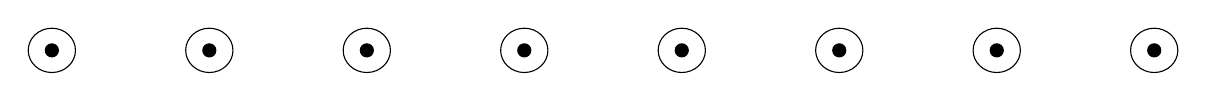
\begin{tikzpicture}[every node/.style={draw}] 
\centering
\node (l1) at (2,0) [circle,fill=black,scale=0.5] {};
\node (l2) at (4,0) [circle,fill=black,scale=0.5] {};
\node (l3) at (6,0) [circle,fill=black,scale=0.5] {};
\node (l4) at (8,0) [circle,fill=black,scale=0.5] {};
\node (l5) at (10,0) [circle,fill=black,scale=0.5] {};
\node (l6) at (12,0) [circle,fill=black,scale=0.5] {};
\node (l7) at (14,0) [circle,fill=black,scale=0.5] {};
\node (l8) at (16,0) [circle,fill=black,scale=0.5] {};

\draw let \p1=(l1), \p2=(l1), \n1={atan2(\y2-\y1,\x2-\x1)}, \n2={veclen(\y2-\y1,\x2-\x1)}
  in ($ (l1)!0.5!(l1) $) ellipse [x radius=\n2/2+8pt, y radius=0.3cm,rotate=0-\n1];
\draw let \p1=(l2), \p2=(l2), \n1={atan2(\y2-\y1,\x2-\x1)}, \n2={veclen(\y2-\y1,\x2-\x1)}
  in ($ (l2)!0.5!(l2) $) ellipse [x radius=\n2/2+8pt, y radius=0.3cm,rotate=0-\n1];
\draw let \p1=(l3), \p2=(l3), \n1={atan2(\y2-\y1,\x2-\x1)}, \n2={veclen(\y2-\y1,\x2-\x1)}
  in ($ (l3)!0.5!(l3) $) ellipse [x radius=\n2/2+8pt, y radius=0.3cm,rotate=0-\n1];
\draw let \p1=(l4), \p2=(l4), \n1={atan2(\y2-\y1,\x2-\x1)}, \n2={veclen(\y2-\y1,\x2-\x1)}
  in ($ (l4)!0.5!(l4) $) ellipse [x radius=\n2/2+8pt, y radius=0.3cm,rotate=0-\n1];
\draw let \p1=(l5), \p2=(l5), \n1={atan2(\y2-\y1,\x2-\x1)}, \n2={veclen(\y2-\y1,\x2-\x1)}
  in ($ (l5)!0.5!(l5) $) ellipse [x radius=\n2/2+8pt, y radius=0.3cm,rotate=0-\n1];
\draw let \p1=(l6), \p2=(l6), \n1={atan2(\y2-\y1,\x2-\x1)}, \n2={veclen(\y2-\y1,\x2-\x1)}
  in ($ (l6)!0.5!(l6) $) ellipse [x radius=\n2/2+8pt, y radius=0.3cm,rotate=0-\n1];
\draw let \p1=(l7), \p2=(l7), \n1={atan2(\y2-\y1,\x2-\x1)}, \n2={veclen(\y2-\y1,\x2-\x1)}
  in ($ (l7)!0.5!(l7) $) ellipse [x radius=\n2/2+8pt, y radius=0.3cm,rotate=0-\n1];
\draw let \p1=(l8), \p2=(l8), \n1={atan2(\y2-\y1,\x2-\x1)}, \n2={veclen(\y2-\y1,\x2-\x1)}
  in ($ (l8)!0.5!(l8) $) ellipse [x radius=\n2/2+8pt, y radius=0.3cm,rotate=0-\n1];
\end{tikzpicture}
\end{center}
  \vskip-0.2cm
  \caption{
 Single non-crossing partition
of $1 \times (k-1)$ with $d=8$.} 
\label{f2-1}
\end{figure}

\vskip-0.4cm

% \section{1d random geometric graphs} 
% \label{s3}
 Given $d\geq 1$, $r_0>$ and $x<y$, let $L_1 , \ldots , L_d$
 be $d$ disjoint intervals of $[x,y]$ 
 with identical lengths $a_k: = kr_0 - (y-x) >0$,
 called cells, and defined as 
\begin{equation}
L_j := B(x,jr_0) \cap B(y,(k-j)r_0), \qquad j = 1,\ldots , r. 
\end{equation}


\begin{eqnarray}
  \nonumber 
      \sigma_k (t)
      & = &
      \int_{t-r}^{(k-1)r}
    \int_{s_{k-1}^--r}^{(k-2)r}
  \cdots
  \int_{s_2^--r}^r dN_{s_1} \cdots dN_{s_{k-1}}
  \\
  \label{fjdksdfa}
  & \stackrel{d}{\simeq} & 
 \int_t^{kr}
 \int_{u_{k-1}^--r}^{(k-1)r}
  \cdots
  \int_{u_2^--r}^{2r} dN_{u_1-r} \cdots dN_{u_{k-1}-r}
, 
\end{eqnarray} 
 where $s_k:=t$, 
 hence the following proposition. % $t\in 
% In the general case, joint moments can be obtained from the following recursion for any number of hops. 



 and 
\begin{equation}
\label{fjlksa2} 
 \widehat{G}(\sigma )
 = \sum_{ \pi \preceq \sigma }
 \sum_{\psi \preceq \pi }
 \mu ( \psi , \pi )
 \widehat{G} (\psi )
 = 
 \sum_{\psi \preceq \pi \preceq \sigma }
 \mu ( \psi , \pi )
 \widehat{G} (\psi )
, 
 \qquad \pi \in \Pi[n]. 
\end{equation} 
 The M\"obius transform can also be defined from the sum
$$ 
 \widecheck{G} (\sigma ) := \sum_{\sigma \preceq \pi } G(\pi ) 
$$ 
 over the partitions
 $\pi$ which are {\em coarser} than $\sigma$,
 in which case it can be inverted as the sum
 over {\em coarser} partitions 
\begin{equation}
\label{gpi} 
 G(\pi) = \sum_{ \pi \preceq \sigma } \mu ( \pi , \sigma ) \widecheck{G} (\sigma), 
\end{equation} 
 using the same M\"obius function $\mu ( \pi , \sigma )$,
 see also \S~2.5 of \cite{peccatitaqqu}.
 In this case, we have
\begin{equation}
\label{gpi3} 
G(\pi) = \sum_{ \pi \preceq \sigma } \mu ( \pi , \sigma )
 \sum_{\sigma \preceq \eta } G(\eta )
= \sum_{\pi \preceq \sigma \preceq \eta } \mu ( \pi , \sigma )
 G(\eta ), 
\end{equation} 
and
\begin{equation}
\label{gpi4} 
\widecheck{G} (\sigma )
= \sum_{\sigma \preceq \pi }
\sum_{ \pi \preceq \eta } \mu ( \pi , \eta ) \widecheck{G} (\eta )
= \sum_{ \sigma \preceq \pi \preceq \eta }
 \mu ( \pi , \eta ) \widecheck{G} (\eta ). 
\end{equation} 


\vspace{-0.6cm}
  \begin{figure}[H]
  \centering
 \begin{subfigure}[b]{0.49\textwidth}
    \includegraphics[width=1\linewidth, height=5cm]{clt_6_hops/graph-6 1 .pdf}
    \caption{10,000 samples.} 
 \end{subfigure}
% \vskip0.1cm
 \begin{subfigure}[b]{0.49\textwidth}
    \includegraphics[width=1\linewidth, height=5cm]{clt_6_hops/graph-6 8 .pdf}
    \caption{80,000 samples.} 
 \end{subfigure}
  % \vskip-0.6cm
  \caption{Convergence of $6$-hop counts.} 
\end{figure}

  and yields \eqref{fjkdsl}.
., when $\lambda_k ( du)=\lambda_k du$, as 
 \begin{equation}
   \label{fjklsdf-11} 
  m_{k,1}^{(m)}(\tau )
=
\lambda_1\cdots \lambda_{k-1} \frac{\tau^{k-1}}{(k-1)!}. 
\end{equation} 


 In particular, Proposition~\ref{jkld} shows that 
$$
\kappa (X_1,X_2 X_3)  = 
\kappa (X_1,X_2,X_3 )
+
\kappa (X_2) \kappa (X_1,X_3)
+
\kappa (X_3) \kappa (X_1,X_2). 
$$ 
% \vskip-1cm


\begin{figure}[H]
  \centering
 \begin{subfigure}[b]{0.49\textwidth}
    \includegraphics[width=1\linewidth, height=5cm]{correl_4_hops/first}
    \caption{First moment of $\sigma_{4,1}(t)$.} 
%    \label{fig:density_quadratic_equilibrium_20person-a} 
 \end{subfigure}
 % \vskip0.1cm
 \begin{subfigure}[b]{0.49\textwidth}
    \includegraphics[width=1\linewidth, height=5cm]{correl_4_hops/second} 
    \caption{Second joint moments of $\sigma_{4,1}()$.} 
 %   \label{fig:density_quadratic_equilibrium_20person-b}
 \end{subfigure}
  % \vskip-0.6cm
  \caption{First and second joint moments of $4$-hop counts.} 
\end{figure}

  \medskip

\begin{center}
\begin{lstlisting}
(*Computation of cumulants*) cn[t__, k_] := (Module[{pt, n, i, j, l, z, temp2}, temp2 = 0;
   n = Length[t]; For[l = 1, l <= n, l++, pt = KSetPartitions[n, l];
    Do[c = 1; For[i = 1, i <= Length[p], i++, z = {};
      For[j = 1, j <= Length[p[[i]]], j++, 
       z = Append[z, t[[p[[i]][[j]]]]]]; c = c*mk[z, k]]; 
     temp2 += c*(-1)^(l - 1)*(l - 1)!, {p, pt}]]; temp2])
\end{lstlisting}
\end{center}

\noindent
\label{Rcode4.00}% \addtocounter{Rcount}{1}
\begin{center}
\begin{minipage}{0.96\linewidth}
\begin{lstlisting}[language=R]
install.packages("diagram")
library(diagram)
r=1;k=5;T=k*r;t=(k-0.5)*r;N=1000;lambda=6;cc=0;s=rexp(1,lambda);
colors=c(2,6,4,7,8,1,3);times=c();
while (s<T) {times=c(times,s);s=s+rexp(1,lambda)}
plot(0, xlim = c(0,T), axes=FALSE, type = "n", xlab = "", ylab = "", yaxs="i")
axis(1, at = c(r*seq(0,k),t),pos=0)
points(times,rep(0,length(times)),pch=16, cex=0.7, col="blue", main="")
for (j in 1:(k-1)) {segments(t-(k-j)*r,-0.1, j*r,-0.1, col= 'pink',lwd=3)}
axis(1, at = c(t-(k-seq(1,k-1))),pos=0)
for (u1 in times) {for (u2 in times) {for (u3 in times) {for (u4 in times) {
if (u1<r && abs(u2-u1)<r && abs(u3-u2)<r && abs(u4-u3)<r && abs(t-u4)<r) {
print(c(u1,u2,u3,u4))
cv=-0.1*(cc+1)
c=colors[1+cc%%6];print(c)
curvedarrow(from = c(0,0), to = c(u1,0), lwd=1.2, curve = cv, arr.type = 'none', arr.pos = 1,lcol=c)
curvedarrow(from = c(u1,0), to = c(u2,0), lwd=1.2, curve = cv, arr.type = 'none', arr.pos = 1,lcol=c)
curvedarrow(from = c(u2,0), to = c(u3,0), lwd=1.2, curve = cv, arr.type = 'none', arr.pos = 1,lcol=c)
curvedarrow(from = c(u3,0), to = c(u4,0), lwd=1.2, curve = cv, arr.type = 'none', arr.pos = 1,lcol=c)
curvedarrow(from = c(u4,0), to = c(t,0), lwd=1.2, curve = cv, arr.type = 'none', arr.pos = 1,lcol=c)
cc=cc+1}}}}}
cat("5-hop count=",cc,"\n")
\end{lstlisting}
\end{minipage}
\end{center}

\vskip-.5cm



\begin{eqnarray*} 
\frac{c_{3,4} (t)}{\big(c_{3,2} (t)\big)^2}
& \leq &
(2(\lambda +1))^5
B_4
 2^{-4}
\frac{3!^2}{\lambda^6 }
\\
& = &
2
(\lambda +1)^{-1} 
(B_4)^{k-2}
3!^2
\\
& = &
2 (\lambda +1)^{-1} 
B_4
3!^2
\\
& = &
2 (\lambda +1)^{-1} 
\frac{4}{\log 4}
3!^2. 
\end{eqnarray*} 



\frac{3!^{n/2}}{\lambda^{3n/2}}
\frac{c_{3,n}(t)}{ 2^n
(3r-\tau)^{3n/2}
}
\\
 & = & 
\frac{3!^{n/2}}{\lambda^{3n/2}}
\frac{O ( (\lambda (3r-\tau))^{ 1 + n })}{ 2^n
(3r-\tau)^{3n/2}
}
\\
& = & O \big( \lambda^{1-n/2} \big)

\vskip-0.8cm

\noindent

 
\begin{table}[H]
\centering 
    \renewcommand{\arraystretch}{2.1}
      \begin{NiceTabular}{c|c|} 
\cline{1-2} % \hline 
\multicolumn{1}{|c|}{$3$-hops} & $0$ 
\\ 
\cline{1-2} % \hline
\multicolumn{1}{|c|}{$4$-hops} & $\displaystyle - \frac{7 t^{10}}{5400} - \frac{t^{11}}{14850}$
\\ 
\cline{1-2} % \hline
\multicolumn{1}{|c|}{$5$-hops} &  $\displaystyle - \frac{2257 t^{14}}{100900800} - \frac{37 t^{15}}{56756700}$ 
\\ 
\cline{1-2}
\multicolumn{1}{|c|}{$6$-hops} &  $\displaystyle % t^5/120 + (7 t^6)/72 + (13 t^7)/28 + (12203 t^8)/10080 + ( 43867 t^9)/22680 + (456217 t^10)/226800 + (1007767 t^11)/712800 + ( 41314769 t^12)/59875200 + (74008043 t^13)/311351040 + ( 63046843 t^14)/1089728640 + (99222007 t^15)/10216206000 + ( 340963009 t^16)/326918592000 + (313754659 t^17)/5557616064000
- \frac{3084841 t^{18}}{33345696384000} - \frac{226703 t^{19}}{126713646259200}$
\\ 
\cline{1-2}
\end{NiceTabular} 
\caption{Fourth cumulant extra terms.} % in seconds.} 
\end{table} 

\vskip-0.3cm



The next bound is valid at the third cumulant order and does not
extend to higher orders.
\begin{prop}
  \label{fjdlsdf} 
  For any $k\geq 2$, for some $C_k>0$ we have the equivalence 
  $$
  c_{k,3} (\tau ,\tau ,\tau ) 
  \simeq 
  C_k ( \lambda \tau )^{3k-5} 
$$
 as $\lambda$ tends to infinity.
\end{prop}
\begin{Proof}
  The bound holds for $k=2$ by the properties of the Poisson cumulants.
  Next, by Proposition~\ref{jkld} we have 
$$
c_{k,3} (u_1,\{1,2\};u_3,\{3\})
=
c_{k,3} (u_1,u_2,u_3) 
+ c_{k,1} (u_2) c_{k,2} (u_1,u_3) 
+ c_{k,1} (u_3) c_{k,2} (u_1,u_2), 
$$
 hence from Proposition~\ref{p1.8} or Proposition~\ref{fjhkds}
 we obtain 
  \begin{eqnarray*} 
  \lefteqn{
    c_{k+1,3} (\tau,\tau,\tau) 
 = \lambda \int_0^\tau 
  c_{k,3} (\tau_1 ,\{1,2,3\}) 
  d\tau_1
  }
  \\
  &
&  + \lambda^2 
  \int_0^\tau 
  \int_0^\tau 
  (
c_{k,3} (\tau_1,\tau_1,\tau_2) 
+ 2 c_{k,1} (\tau_1) c_{k,2} (\tau_1,\tau_2) 
) 
  d\tau_1 d\tau_3
  \\
  & & 
  + 
  2 \lambda^2 \int_0^\tau 
  \int_0^\tau
  (
  c_{k,3} (\tau_1,\tau_1,\tau_3) 
+ 2 c_{k,1} (\tau_1) c_{k,2} (\tau_1,\tau_3) 
) 
  d\tau_1 d\tau_3
  \\
  & & 
 + \lambda^3 
  \int_0^\tau 
  \int_0^\tau 
  \int_0^\tau 
  c_{k,3} (\tau_1,\tau_2,\tau_3) 
  d\tau_1 d\tau_2 d\tau_3 
  \\
  & = & O((\lambda \tau )^{3(k-1)+1} )
  \\
  & &
  + 
  3\lambda^2 \int_0^\tau 
  \int_0^\tau 
  (
  O((\lambda \tau)^{3k-5})
  + 2 O((\lambda \tau )^{k-1})O((\lambda \tau )^{2k-3})
%  c_{k,1} (\tau_1) c_{k,2} (\tau_1,\tau_2) 
) 
  d\tau_1 d\tau_3
  \\
  & &
  + \lambda^3 
  \int_0^\tau 
  \int_0^\tau 
  \int_0^\tau 
  O((\lambda \tau)^{3k-5})
  d\tau_1 d\tau_2 d\tau_3 
  \\
  & = & O((\lambda \tau )^{3(k-1)+1} )
  + 
  3  O((\lambda \tau)^{3k-3})
  +
  6 O((\lambda \tau )^{3k-2}
  + 
  O((\lambda \tau)^{3k-2})
  \\
  & = &
  O((\lambda \tau)^{3(k+1)-5})
. 
\end{eqnarray*} 
\end{Proof}
  \noindent 
  We note that the argument of Proposition~\ref{fjdlsdf} does not
  extend to fourth order cumulants. Indeed,
  from the relation 
\begin{eqnarray*} 
\kappa (X_1,X_2, X_3X_4) & = &  
\kappa (X_1,X_2,X_3 ,X_4)
\\
 & & +
\kappa (X_3) \kappa (X_1,X_3,X_4)
+
\kappa (X_4) \kappa (X_1,X_2,X_3) 
\\
 & & +
\kappa (X_1,X_3) \kappa (X_2,X_4)
+
\kappa (X_1,X_4) \kappa (X_2,X_3) 
\end{eqnarray*} 
 and Proposition~\ref{fjhkds}
 we have
\begin{eqnarray*}
 c_{k+1,4} (\tau ,\ldots , \tau )
 & = & 
  \lambda 
  \int_0^\tau 
  c_{k,1} (\tau_1,\{1,2,3,4\}) d\tau_1 
  \\
   & & + 
  \lambda^2
  \sum_{\pi_1\cup \pi_2 = \{1,2,3,4\} }
  \int_0^\tau \int_0^\tau 
  c_{k,2} (\tau_1,\pi_1; \tau_2,\pi_2) 
  d\tau_1 d\tau_2 
\\ 
   &  & +  
  \lambda^3
  \sum_{\pi_1\cup \pi_2 \cup \pi_3  = \{1,2,3,4\} }
  \int_0^\tau \int_0^\tau \int_0^\tau 
  c_{k,3} (\tau_1,\pi_1; \tau_2,\pi_2; \tau_3,\pi_4) 
  d\tau_1   d\tau_2   d\tau_3 
\\ 
   &  & +  
  \lambda^4
  \int_0^\tau \int_0^\tau \int_0^\tau \int_0^\tau 
  c_{k,4} (\tau_1,\{1\};\tau_2,\{2\};\tau_3,\{3\};\tau_4,\{4\}) 
  d\tau_1 d\tau_2 d\tau_3 d\tau_4 
.
\end{eqnarray*} 
In particular, we have
\begin{eqnarray*}
  \lefteqn{
    \lambda^3
  \int_0^\tau \int_0^\tau \int_0^\tau 
  c_{k,3} (\tau_1,\{1\}; \tau_2,\{2\}; \tau_3,\{3,4\}) 
  d\tau_1   d\tau_2   d\tau_3 
  }
  \\
  & = & 
  \lambda^3
  \int_0^\tau \int_0^\tau \int_0^\tau 
  c_{k,3} (\tau_1,\{1\}; \tau_2,\{2\}; \tau_3,\{3,4\}) 
  d\tau_1   d\tau_2   d\tau_3 
\\
  & = & 
  ( \lambda \tau )^3
\times ( \lambda \tau )
\times ( \lambda \tau )^{3k-5}
\\
  & = & 
 ( \lambda \tau )^{3(k+1)-4}, 
\end{eqnarray*} 
which is consistent with the higher order terms
$36\tau^5/5$ and $-\tau^{11}/14850$ in 
for $k=3$ and $k=4$ in Tables~\ref{table6} and \ref{table7}. 

\hskip-10cm
\scriptsize
\begin{eqnarray*} 
\lefteqn{
 \kappa_{k+1,4} (t_1,t_2,t_3,t_4) 
 = 
 \sum_{l=1}^n
  (l-1)!
  (-1)^{l-1}
  \sum_{\pi_1\cup \cdots \cup \pi_l = \{1,\ldots , n\}}
  \prod_{j=1}^l 
  m_{k+1,|\pi_j|} (\widehat{s}_{\pi_j})
  }
  \\
& = &  
  m_{k+1,4} (t_1,t_2,t_3,t_4) 
  \\
  & & 
  - 
  m_{k+1,1} (t_1)m_{k+1,3} (t_2,t_3,t_4) 
  - 
  m_{k+1,1} (t_2)m_{k+1,3} (t_1,t_3,t_4) 
  - 
  m_{k+1,1} (t_3)m_{k+1,3} (t_1,t_2,t_4) 
  - 
  m_{k+1,1} (t_4)m_{k+1,3} (t_1,t_2,t_3) 
  \\
  & & 
  - 
  m_{k+1,2} (t_1,t_2)m_{k+1,2} (t_3,t_4) 
  - 
  m_{k+1,2} (t_1,t_3)m_{k+1,2} (t_2,t_4) 
  - 
  m_{k+1,2} (t_2,t_3)m_{k+1,2} (t_1,t_4) 
  \\
  & & 
  + 
  2m_{k+1,1} (t_1)m_{k+1,1} (t_2)m_{k+1,2} (t_3,t_4) 
  + 
  2m_{k+1,1} (t_1)m_{k+1,1} (t_3)m_{k+1,2} (t_2,t_4) 
  + 
  2m_{k+1,1} (t_1)m_{k+1,1} (t_4)m_{k+1,2} (t_2,t_3) 
  \\
  & &
  + 
  2m_{k+1,1} (t_2)m_{k+1,1} (t_3)m_{k+1,2} (t_1,t_4) 
    + 
  2m_{k+1,1} (t_2)m_{k+1,1} (t_4)m_{k+1,2} (t_1,t_3) 
    + 
  2m_{k+1,1} (t_3)m_{k+1,1} (t_4)m_{k+1,2} (t_1,t_2) 
  \\
  & &
  - 6 m_{k+1,1} (t_1)m_{k+1,1} (t_2)m_{k+1,1} (t_3)m_{k+1,1} (t_4)
\\
& = &  
  \int_0^{t_1} 
  m_{k,4} (u_1) 
  \lambda_k (du_1) 
  \\
  & &
  +
  \int_0^{t_1} 
  \int_0^{\min ( t_2,t_3,t_4)}
  m_{k,4} (u_1,u_2,u_2,u_2) 
  du_1du_2 
  +
  \int_0^{t_2} 
  \int_0^{\min ( t_1,t_3,t_4)}
  m_{k,4} (u_2,u_1,u_2,u_2) 
  du_1du_2 
  +
  \int_0^{t_3} 
  \int_0^{\min ( t_1,t_2,t_4)}
  m_{k,4} (u_2,u_2,u_1,u_2) 
  du_1du_2 
  +
  \int_0^{t_4} 
  \int_0^{\min ( t_1,t_2,t_3)}
  m_{k,4} (u_2,u_2,u_2,u_1) 
  du_1du_2 
 \\
  & &
  +
  \int_0^{\min (t_1,t_2)} 
  \int_0^{\min (t_3,t_4)} 
  m_{k,4} (u_1,u_1,u_2,u_2) 
  du_1du_2 
  +
  \int_0^{\min (t_1,t_3)} 
  \int_0^{\min (t_2,t_4)} 
  m_{k,4} (u_1,u_2,u_1,u_2) 
  du_1du_2 
  +
  \int_0^{\min (t_2,t_3)} 
  \int_0^{\min (t_1,t_4)} 
  m_{k,4} (u_1,u_2,u_2,u_1) 
  du_1du_2 
\\
  & &
  +
  \int_0^{t_1} 
  \int_0^{t_2}
  \int_0^{\min ( t_3,t_4)}
  m_{k,4} (u_1,u_2,u_3,u_3) 
  du_1du_2du_3
  +
  \int_0^{t_1} 
  \int_0^{t_3}
  \int_0^{\min ( t_2,t_4)}
  m_{k,4} (u_1,u_2,u_3,u_2) 
  du_1du_2du_3
  +
  \int_0^{t_1} 
  \int_0^{t_4}
  \int_0^{\min ( t_2,t_3)}
  m_{k,4} (u_1,u_2,u_2,u_3) 
  du_1du_2du_3
  \\
  & & 
  +
  \int_0^{t_2} 
  \int_0^{t_3}
  \int_0^{\min ( t_1,t_4)}
  m_{k,4} (u_1,u_2,u_3,u_1) 
  du_1du_2du_3
  +
  \int_0^{t_2} 
  \int_0^{t_4}
  \int_0^{\min ( t_1,t_3)}
  m_{k,4} (u_1,u_2,u_1,u_4) 
  du_1du_2du_3
  +
  \int_0^{t_3} 
  \int_0^{t_4}
  \int_0^{\min ( t_1,t_3)}
  m_{k,4} (u_1,u_2,u_3,u_3) 
  du_1du_2du_3
\\
  & & 
    +
  \int_0^{t_1} 
  \int_0^{t_2} 
  \int_0^{t_3} 
  \int_0^{t_4} 
  m_{k,4} (u_1,u_2,u_3,u_4) 
  du_1du_2du_3du_4
  \\
  & & 
  - 
  m_{k+1,1} (t_1)m_{k+1,3} (t_2,t_3,t_4) 
  - 
  m_{k+1,1} (t_2)m_{k+1,3} (t_1,t_3,t_4) 
  - 
  m_{k+1,1} (t_3)m_{k+1,3} (t_1,t_2,t_4) 
  - 
  m_{k+1,1} (t_4)m_{k+1,3} (t_1,t_2,t_3) 
  \\
  & & 
  - 
  m_{k+1,2} (t_1,t_2)m_{k+1,2} (t_3,t_4) 
  - 
  m_{k+1,2} (t_1,t_3)m_{k+1,2} (t_2,t_4) 
  - 
  m_{k+1,2} (t_2,t_3)m_{k+1,2} (t_1,t_4) 
  \\
  & & 
  + 
  2m_{k+1,1} (t_1)m_{k+1,1} (t_2)m_{k+1,2} (t_3,t_4) 
  + 
  2m_{k+1,1} (t_1)m_{k+1,1} (t_3)m_{k+1,2} (t_2,t_4) 
  + 
  2m_{k+1,1} (t_1)m_{k+1,1} (t_4)m_{k+1,2} (t_2,t_3) 
  \\
  & &
  + 
  2m_{k+1,1} (t_2)m_{k+1,1} (t_3)m_{k+1,2} (t_1,t_4) 
    + 
  2m_{k+1,1} (t_2)m_{k+1,1} (t_4)m_{k+1,2} (t_1,t_3) 
    + 
  2m_{k+1,1} (t_3)m_{k+1,1} (t_4)m_{k+1,2} (t_1,t_2) 
  \\
  & &
  - 6 m_{k+1,1} (t_1)m_{k+1,1} (t_2)m_{k+1,1} (t_3)m_{k+1,1} (t_4)
  \\
& = &  
  \int_0^{t_1} 
  m_{k,4} (u_1) 
  \lambda_k (du_1) 
  \\
  & &
  +
  \int_0^{t_1} 
  \int_0^{\min ( t_2,t_3,t_4)}
  m_{k,4} (u_1,u_2,u_2,u_2) 
  du_1du_2 
  +
  \int_0^{t_2} 
  \int_0^{\min ( t_1,t_3,t_4)}
  m_{k,4} (u_2,u_1,u_2,u_2) 
  du_1du_2 
  +
  \int_0^{t_3} 
  \int_0^{\min ( t_1,t_2,t_4)}
  m_{k,4} (u_2,u_2,u_1,u_2) 
  du_1du_2 
  +
  \int_0^{t_4} 
  \int_0^{\min ( t_1,t_2,t_3)}
  m_{k,4} (u_2,u_2,u_2,u_1) 
  du_1du_2 
 \\
  & &
  +
  \int_0^{\min (t_1,t_2)} 
  \int_0^{\min (t_3,t_4)} 
  m_{k,4} (u_1,u_1,u_2,u_2) 
  du_1du_2 
  +
  \int_0^{\min (t_1,t_3)} 
  \int_0^{\min (t_2,t_4)} 
  m_{k,4} (u_1,u_2,u_1,u_2) 
  du_1du_2 
  +
  \int_0^{\min (t_2,t_3)} 
  \int_0^{\min (t_1,t_4)} 
  m_{k,4} (u_1,u_2,u_2,u_1) 
  du_1du_2 
\\
  & &
  +
  \int_0^{t_1} 
  \int_0^{t_2}
  \int_0^{\min ( t_3,t_4)}
  m_{k,4} (u_1,u_2,u_3,u_3) 
  du_1du_2du_3
  +
  \int_0^{t_1} 
  \int_0^{t_3}
  \int_0^{\min ( t_2,t_4)}
  m_{k,4} (u_1,u_2,u_3,u_2) 
  du_1du_2du_3
  +
  \int_0^{t_1} 
  \int_0^{t_4}
  \int_0^{\min ( t_2,t_3)}
  m_{k,4} (u_1,u_2,u_2,u_3) 
  du_1du_2du_3
  \\
  & & 
  +
  \int_0^{t_2} 
  \int_0^{t_3}
  \int_0^{\min ( t_1,t_4)}
  m_{k,4} (u_1,u_2,u_3,u_1) 
  du_1du_2du_3
  +
  \int_0^{t_2} 
  \int_0^{t_4}
  \int_0^{\min ( t_1,t_3)}
  m_{k,4} (u_1,u_2,u_1,u_4) 
  du_1du_2du_3
  +
  \int_0^{t_3} 
  \int_0^{t_4}
  \int_0^{\min ( t_1,t_3)}
  m_{k,4} (u_1,u_2,u_3,u_3) 
  du_1du_2du_3
\\
  & & 
    +
  \int_0^{t_1} 
  \int_0^{t_2} 
  \int_0^{t_3} 
  \int_0^{t_4} 
  c_{k,4} (u_1,u_2,u_3,u_4) 
  du_1du_2du_3du_4
  \\
  & & 
  - 
  m_{k+1,1} (t_1)\left(
  \int_0^{\min (t_1,t_2)} 
  \int_0^{t_3} 
  m_{k,3} (u_1,u_1,u_3) 
  \lambda_k (du_1) \lambda_k (du_3)
  + 
  \int_0^{\min (t_1,t_3)} 
  \int_0^{t_2} 
  m_{k,3} (u_1,u_2,u_1) 
  \lambda_k (du_1) \lambda_k (du_2)
  + 
  \int_0^{t_1}
  \int_0^{\min (t_2,t_3)} 
  m_{k,3} (u_1,u_2,u_2) 
  \lambda_k (du_1) (du_2)
   + 
  \int_0^{t_1} 
  \int_0^{t_2} 
  \int_0^{t_3} 
  m_{k,3} (u_1,u_2,u_3) 
  \lambda_k (du_1) \lambda_k (du_2) \lambda_k (du_3) 
  \right) 
\\
 & & - 
  m_{k+1,1} (t_2)m_{k+1,3} (t_1,t_3,t_4) 
  - 
  m_{k+1,1} (t_3)m_{k+1,3} (t_1,t_2,t_4) 
  - 
  m_{k+1,1} (t_4)m_{k+1,3} (t_1,t_2,t_3) 
  \\
  & & 
  - 
  m_{k+1,2} (t_1,t_2)
  \left(
      \int_0^{t_2}
  m_{k,2} (u_1, u_1 ) 
  \lambda_k (du_1) 
\textcolor{red}{ + \int_0^{t_2} \int_0^{t_3} m_{k,2} (u_1, u_2 ) \lambda_k (du_1) \lambda_k (du_2)}
\right) 
  - 
  m_{k+1,2} (t_1,t_3)m_{k+1,2} (t_2,t_4) 
  - 
  m_{k+1,2} (t_2,t_3)m_{k+1,2} (t_1,t_4) 
  \\
  & & 
  + 
  2m_{k+1,1} (t_1)m_{k+1,1} (t_2)
    \left(
      \int_0^{t_3}
  m_{k,2} (u_1, u_1 ) 
  \lambda_k (du_1) 
% + \int_0^{t_3} \int_0^{t_4} m_{k,2} (u_1, u_2 ) \lambda_k (du_1) \lambda_k (du_2)
\right) 
  + 
  2m_{k+1,1} (t_1)m_{k+1,1} (t_3)m_{k+1,2} (t_2,t_4) 
  + 
  2m_{k+1,1} (t_1)m_{k+1,1} (t_4)m_{k+1,2} (t_2,t_3) 
  \\
  & &
  + 
  2m_{k+1,1} (t_2)m_{k+1,1} (t_3)m_{k+1,2} (t_1,t_4) 
    + 
  2m_{k+1,1} (t_2)m_{k+1,1} (t_4)m_{k+1,2} (t_1,t_3) 
    + 
  2m_{k+1,1} (t_3)m_{k+1,1} (t_4)m_{k+1,2} (t_1,t_2) 
 \\
& = &  
  \int_0^{t_1} 
  m_{k,4} (u_1) 
  \lambda_k (du_1) 
  \\
  & &
  +
  \int_0^{t_1} 
  \int_0^{\min ( t_2,t_3,t_4)}
  m_{k,4} (u_1,u_2,u_2,u_2) 
  du_1du_2 
  +
  \int_0^{t_2} 
  \int_0^{\min ( t_1,t_3,t_4)}
  m_{k,4} (u_2,u_1,u_2,u_2) 
  du_1du_2 
  +
  \int_0^{t_3} 
  \int_0^{\min ( t_1,t_2,t_4)}
  m_{k,4} (u_2,u_2,u_1,u_2) 
  du_1du_2 
  +
  \int_0^{t_4} 
  \int_0^{\min ( t_1,t_2,t_3)}
  m_{k,4} (u_2,u_2,u_2,u_1) 
  du_1du_2 
 \\
  & &
  +
  \int_0^{\min (t_1,t_2)} 
  \int_0^{\min (t_3,t_4)} 
  m_{k,4} (u_1,u_1,u_2,u_2) 
  du_1du_2 
  +
  \int_0^{\min (t_1,t_3)} 
  \int_0^{\min (t_2,t_4)} 
  m_{k,4} (u_1,u_2,u_1,u_2) 
  du_1du_2 
  +
  \int_0^{\min (t_2,t_3)} 
  \int_0^{\min (t_1,t_4)} 
  m_{k,4} (u_1,u_2,u_2,u_1) 
  du_1du_2 
\\
  & &
  +
  \int_0^{t_1} 
  \int_0^{t_2}
  \int_0^{\min ( t_3,t_4)}
  c_{k,4} (u_1,u_2,u_3,u_3) 
  du_1du_2du_3
  +
  \int_0^{t_1} 
  \int_0^{t_3}
  \int_0^{\min ( t_2,t_4)}
  c_{k,4} (u_1,u_2,u_3,u_2) 
  du_1du_2du_3
  +
  \int_0^{t_1} 
  \int_0^{t_4}
  \int_0^{\min ( t_2,t_3)}
  c_{k,4} (u_1,u_2,u_2,u_3) 
  du_1du_2du_3
  \\
  & & 
  +
  \int_0^{t_2} 
  \int_0^{t_3}
  \int_0^{\min ( t_1,t_4)}
  c_{k,4} (u_1,u_2,u_3,u_1) 
  du_1du_2du_3
  +
  \int_0^{t_2} 
  \int_0^{t_4}
  \int_0^{\min ( t_1,t_3)}
  m_{k,4} (u_1,u_2,u_1,u_4) 
  du_1du_2du_3
  +
  \int_0^{t_3} 
  \int_0^{t_4}
  \int_0^{\min ( t_1,t_3)}
  c_{k,4} (u_1,u_2,u_3,u_3) 
  du_1du_2du_3
\\
  & & 
    +
  \int_0^{t_1} 
  \int_0^{t_2} 
  \int_0^{t_3} 
  \int_0^{t_4} 
  c_{k,4} (u_1,u_2,u_3,u_4) 
  du_1du_2du_3du_4
  \\
  & & 
  - 
  m_{k+1,1} (t_1)\left(
  \int_0^{t_1} 
    m_{k,3} (u_1,u_1,u_1) 
  \lambda_k (du_1) 
  \right) 
\\
 & & - 
  m_{k+1,1} (t_2)m_{k+1,3} (t_1,t_3,t_4) 
  - 
  m_{k+1,1} (t_3)m_{k+1,3} (t_1,t_2,t_4) 
  - 
  m_{k+1,1} (t_4)m_{k+1,3} (t_1,t_2,t_3) 
  \\
  & & 
  - 
  m_{k+1,2} (t_1,t_2)
  \left(
      \int_0^{t_2}
  m_{k,2} (u_1, u_1 ) 
  \lambda_k (du_1) 
\textcolor{red}{ + \int_0^{t_2} \int_0^{t_3} m_{k,2} (u_1, u_2 ) \lambda_k (du_1) \lambda_k (du_2)}
\right) 
  - 
  m_{k+1,2} (t_1,t_3)m_{k+1,2} (t_2,t_4) 
  - 
  m_{k+1,2} (t_2,t_3)m_{k+1,2} (t_1,t_4) 
 \\
& = &  
  \int_0^{t_1} 
  m_{k,4} (u_1) 
  \lambda_k (du_1) 
  \\
  & &
  +
  \int_0^{t_1} 
  \int_0^{\min ( t_2,t_3,t_4)}
  c_{k,4} (u_1,u_2,u_2,u_2) 
  du_1du_2 
  +
  \int_0^{t_2} 
  \int_0^{\min ( t_1,t_3,t_4)}
  m_{k,4} (u_2,u_1,u_2,u_2) 
  du_1du_2 
  +
  \int_0^{t_3} 
  \int_0^{\min ( t_1,t_2,t_4)}
  c_{k,4} (u_2,u_2,u_1,u_2) 
  du_1du_2 
  +
  \int_0^{t_4} 
  \int_0^{\min ( t_1,t_2,t_3)}
  c_{k,4} (u_2,u_2,u_2,u_1) 
  du_1du_2 
 \\
  & &
  +
  \int_0^{\min (t_1,t_2)} 
  \int_0^{\min (t_3,t_4)} 
  c_{k,4} (u_1,u_1,u_2,u_2) 
  du_1du_2 
  +
  \int_0^{\min (t_1,t_3)} 
  \int_0^{\min (t_2,t_4)} 
  c_{k,4} (u_1,u_2,u_1,u_2) 
  du_1du_2 
  +
  \int_0^{\min (t_2,t_3)} 
  \int_0^{\min (t_1,t_4)} 
  c_{k,4} (u_1,u_2,u_2,u_1) 
  du_1du_2 
\\
  & &
  +
  \int_0^{t_1} 
  \int_0^{t_2}
  \int_0^{\min ( t_3,t_4)}
  c_{k,4} (u_1,u_2,u_3,u_3) 
  du_1du_2du_3
  +
  \int_0^{t_1} 
  \int_0^{t_3}
  \int_0^{\min ( t_2,t_4)}
  c_{k,4} (u_1,u_2,u_3,u_2) 
  du_1du_2du_3
  +
  \int_0^{t_1} 
  \int_0^{t_4}
  \int_0^{\min ( t_2,t_3)}
  c_{k,4} (u_1,u_2,u_2,u_3) 
  du_1du_2du_3
  \\
  & & 
  +
  \int_0^{t_2} 
  \int_0^{t_3}
  \int_0^{\min ( t_1,t_4)}
  c_{k,4} (u_1,u_2,u_3,u_1) 
  du_1du_2du_3
  +
  \int_0^{t_2} 
  \int_0^{t_4}
  \int_0^{\min ( t_1,t_3)}
  m_{k,4} (u_1,u_2,u_1,u_4) 
  du_1du_2du_3
  +
  \int_0^{t_3} 
  \int_0^{t_4}
  \int_0^{\min ( t_1,t_3)}
  c_{k,4} (u_1,u_2,u_3,u_3) 
  du_1du_2du_3
\\
  & & 
    +
  \int_0^{t_1} 
  \int_0^{t_2} 
  \int_0^{t_3} 
  \int_0^{t_4} 
  c_{k,4} (u_1,u_2,u_3,u_4) 
  du_1du_2du_3du_4
  \\
  & & 
  - 
   \left(
   \textcolor{red}{ \int_0^{t_2} \int_0^{t_3} m_{k,2} (u_1, u_2 ) \lambda_k (du_1) \lambda_k (du_2)}
\right) 
 \left(
   \textcolor{red}{ \int_0^{t_2} \int_0^{t_3} m_{k,2} (u_1, u_2 ) \lambda_k (du_1) \lambda_k (du_2)}
\right) 
  - 
  m_{k+1,2} (t_1,t_3)m_{k+1,2} (t_2,t_4) 
  - 
  m_{k+1,2} (t_2,t_3)m_{k+1,2} (t_1,t_4) 
  \\
  & & + 12
  \\
  & & - 6
  , 
\end{eqnarray*} 

\normalsize



As the leading term is obtained for $l=1$, we have by induction 
   \begin{equation}
     \label{ckn}
c^{(n)}_k (s,\ldots , s) = O ( (\lambda s)^{ 1 + (k-2)n }). 
\end{equation} 


   $$ 
 \kappa \big(Z_1^{l_1},\ldots , X_n^{l_n}\big) 
 = 
 \sum_{l=1}^n
  (l-1)!
  (-1)^{l-1}
  \sum_{\pi_1\cup \cdots \cup \pi_l = \{1,\ldots , n\}}
  \prod_{j=1}^l 
  \E_m  \Bigg[ \prod_{i\in \pi_j} Z_i^{l_i} \Bigg], 
$$


  \int_0^{\tau_1} 
  m_{k,3} (u_1, u_1,u_1 ) 
  \lambda_k (du_1) 
   \\
  & \quad 
  + 
  \sum_{\pi_1\cup \pi_2 = \{ 1,2,3\} }
  \int_0^{\widehat{\tau}_{\pi_1}} 
  \int_0^{\widehat{tau}_{\pi_2}} 
  m_{k,2} (u_1,\pi_1;u_2,\pi_2) 
  \lambda_k (du_1) \lambda_k (du_2)
  \\
  &  \quad  + 
  \int_0^{\tau_1} 
  \int_0^{\tau_2} 
  \int_0^{\tau_3} 
  m_{k,3} (u_1,u_2,u_3) 
  \lambda_k (du_1) \lambda_k (du_2) \lambda_k (du_3) 
  \\
  &  \quad  
  - 
  \int_0^{\tau_1}
  m_{k,1} (u_1 ) 
  \lambda_k (du_1)
  \left(
      \int_0^{\tau_2}
  m_{k,2} (u_1, u_1 ) 
  \lambda_k (du_1) 
 + 
   \int_0^{\tau_2} 
   \int_0^{\tau_3} 
  m_{k,2} (u_1, u_2 ) 
  \lambda_k (du_1) \lambda_k (du_2)
  \right)
  \\
  &  \quad 
   - 
  \int_0^{\tau_2}
  m_{k,1} (u_1 ) 
  \lambda_k (du_1)
\left(
      \int_0^{\tau_1}
  m_{k,2} (u_1, u_1 ) 
  \lambda_k (du_1) 
 + 
   \int_0^{\tau_1} 
   \int_0^{\tau_3} 
  m_{k,2} (u_1, u_2 ) 
  \lambda_k (du_1) \lambda_k (du_2)
  \right)
  \\
  &  \quad  
 - 
  \int_0^{\tau_1}
  m_{k,1} (u_1 ) 
  \lambda_k (du_1)
  \left(
      \int_0^{\tau_2}
  m_{k,2} (u_1, u_1 ) 
  \lambda_k (du_1) 
 + 
   \int_0^{\tau_2} 
   \int_0^{\tau_3} 
  m_{k,2} (u_1, u_2 ) 
  \lambda_k (du_1) \lambda_k (du_2)
  \right)
  \\
   &  \quad  + 2 
  \int_0^{\tau_1}
  m_{k,1} (u_1 ) 
  \lambda_k (du_1)
    \int_0^{\tau_2}
  m_{k,1} (u_2 ) 
  \lambda_k (du_2)
    \int_0^{\tau_3}
  m_{k,1} (u_3 ) 
  \lambda_k (du_3)
     \\
     &


     where 
$$
  m_{k,2} (u_1,u_2) 
  =  \E_m  [ \sigma_k(kr- u_1) \sigma_k(kr-u_2) ],
 \qquad 0 \leq u_1, u_2 \leq r. 
$$


 $$
\int_{[0,t_1]}
  \cdots
  \int_{[0,t_n]}
  m_{1,n} (u_1,\ldots , u_n ) 
  \lambda_1 (du_1) \cdots \lambda_1 (du_n)
$$

\noindent
 As a consequence of Corollary~\ref{c1} and the It\^o isometry
for multiple Poisson stochastic integrals, we obtain the
 first and second moments of the count $\sigma_k(t)$ of $k$-hop paths. 
 Higher cumulants and moments of $\sigma_k(t)$ can
 in principle be computed by this method
 using Corollary~\ref{c1} above and Corollary~7.4.1 of
 \cite{peccatitaqqu}. 
\begin{prop} 
\label{djklfs2-3}
The variance 
of the $k$-hop path count $\sigma_k(kr-\tau)$, $t\in [0,r]$, is given by
 $$ 
 \Var_\lambda  [ \sigma_k (kr-\tau)]
  =
  \sum_{l=1}^{k-1}
  t^{2k-2-l}
  \frac{  \lambda_1^2\cdots \lambda_{k-1}^2}{(2k-2-l)!} 
  \sum_{ j_0 + \cdots + j_l = k-1-l \atop j_0,\ldots , j_l\geq 0}
  \prod_{q=1}^l \frac{1}{\lambda_{j_0+\cdots + j_{q-1}+q}}
  \prod_{{q'}=0}^l {2j_{q'} \choose j_{q'}} 
. 
$$
\end{prop}
\begin{Proof}
 By the It\^o isometry and orthogonality of multiple Poisson
   stochastic integrals, we have
    \begin{align*} 
 & 
    \E_m  [ \sigma_k^2 (t) ] 
    \\
   & = 
 \frac{1}{(k-1)!^2} \sum_{l=0}^{k-1}
   l! {k-1 \choose l}^2
\int_{t-r}^{kr} \cdots \int_{t-r}^{kr}
\left(
\int_{t-r}^{kr} \cdots \int_{t-r}^{kr}
   f_k (s_1,\ldots , s_l , s_{l+1}, \ldots , s_{k-1} ) 
   \right)^2
     ds_1\cdots ds_{k-1}. 
\end{align*} 
  We have
\begin{align*} 
& \sigma_k (t) = 
  \int_{t-r}^{(k-1)r} 
  \int_{s_{k-1}^--r}^{(k-2)r}
  \cdots
  \int_{s_2^--r}^r dN_{s_1} \cdots dN_{s_{k-1}}
\\
 & = 
 \sum_{l=0}^{k-1}
 \sum_{
   0=i_0<i_1< \cdots < i_l <i_{l+1}= k}
 \int_0^{(k-1)r} 
  \cdots
 \int_0^{(k-1)r} 
  f_k(s_1,\ldots ,s_{k-1})
   \prod_{1\leq q \leq d \atop
     q\notin \{i_1,\ldots ,i_l\}}
   \hskip-0.3cm
   (\lambda_q ds_q) 
   \prod_{p=1}^l 
  (dN_{s_{i_p}} -\lambda_{i_p}ds_{i_p}), 
\end{align*} 
hence since $s_i\in [(i-1)r,ir]$, $i=1,\ldots , k-1$, we have 
\begin{align*} 
& \E_m  [\sigma_k^2 (kr-\tau) ] 
  = 
 \sum_{l=0}^{k-1}
  \sum_{
  0=i_0<i_1< \cdots < i_l <i_{l+1}= k}
  \int_{X^l}
  \bigg( 
  \int_{X^{d-l}} 
  f_k(s_1,\ldots ,s_{k-1})
   \prod_{1\leq q < k \atop
     q\notin \{i_1,\ldots ,i_l\}}
   \hskip-0.3cm
  (\lambda_q ds_q)
  \bigg)^2
   \prod_{p=1}^l 
  (\lambda_{i_p}ds_{i_p}). 
\end{align*} 
\end{Proof} 



of the form 
$$
 \lambda (ds) = \sum_{l=1}^k {\bf 1}_{ ( (l-1)r,lr]}(s) \lambda_l((l-1)r + ds), 
$$
 where $\lambda_1(ds), \ldots , \lambda_k(ds)$ are
 intensity measures on the intervals $[(l-1)r,lr]$
 called cells, $l=1,\ldots , k$,


 we find
\begin{align*}
 & 
  c_{k,3} (t_1,t_2,t_3)  = 
  \int_0^{t_1} 
  c_{k,3} (u_1, u_1,u_1 ) 
  \lambda_k (du_1) 
  \\
  &  \quad 
  + 
  \int_0^{t_1} 
  \int_0^{t_3} 
  c_{k,3} (u_1,u_1,u_3) 
  \lambda_k (du_1) \lambda_k (du_3)
  \\
  &  \quad 
  + 
  \int_0^{t_1} 
  \int_0^{t_2} 
  c_{k,3} (u_1,u_2,u_1) 
  \lambda_k (du_1) \lambda_k (du_2)
  \\
  &  \quad 
  + 
  \int_0^{t_1}
  \int_0^{t_2} 
  c_{k,3} (u_1,u_2,u_2) 
  \lambda_k (du_1) (du_2)
  \\
  &  \quad  + 
  \int_0^{t_1} 
  \int_0^{t_2} 
  \int_0^{t_3} 
  c_{k,3} (u_1,u_2,u_3) 
  \lambda_k (du_1) \lambda_k (du_2) \lambda_k (du_3) 
. 
\end{align*} 

\begin{prop}
  \label{pfjkd}
  The joint moments
$$
  m_{k,n}(s_1,\ldots , s_n)
  :=
  \E_m  \big[ Z^{(k)}_{s_1} \cdots Z^{(k)}_{s_n} \big] 
$$
 of the multiple stochastic integral 
$$ 
 Z^{(k)}_t := \int_0^t \int_0^{s_{k-1}^-} \cdots \int_0^{s_2^-} dN^{(1)}_{s_1} \cdots dN^{(k-1)}_{s_{k-1}},
% \quad (k-1)r \leq t \leq kr, 
$$
 where $(N^{(l)}_s)_{s\in \real_+}$ is a family of
 independent Poisson processes with respective intensities $\lambda_l$, $1\leq l \leq r$,
 satisfies the induction relation 
 \begin{equation}
   \label{kldsf}
  m_{k+1,n}(s_1,\ldots , s_n)  = 
  \sum_{l=1}^n
  \sum_{\pi_1\cup \cdots \cup \pi_l = \{1,\ldots , n\}}
  \int_{[0,\widehat{s}_{\pi_l}]}
  \cdots
  \int_{[0,\widehat{s}_{\pi_1}]}
  m_{k,n}^{|\pi|} (u_1,\ldots , u_l ) 
  \lambda_k ( du_1)\cdots \lambda_k (du_l), 
\end{equation} 
 $s_1 , \ldots , s_n\geq 0$. 
% $0\leq s_1\leq \cdots \leq s_n$. 
%  where $\min \pi_i := \min \{ j\in \pi_i\}$, $i=1,\ldots , |\pi|$. 
\end{prop}


\subsubsection*{Sums over partitions}

In the sequel we will use the notation
$$
\sum_{l=1}^n
  \sum_{\pi_1\cup \cdots \cup \pi_l = \{1,\ldots , n\}}
  \int_{\real_+^l} 
  f_{(\pi_1,\ldots , \pi_l)} (u_1,\ldots , u_l ) 
  du_1 \cdots du_l
  =
 \sum_{\pi \in \Pi [n] }
 \int_{\real_+^{||\pi ||}} 
 f_{\pi } \big( ( s_\rho)_{\rho \in \pi} \big) 
 \prod_{\rho \in \pi}
 ds_\rho
$$
 for sums of integrals
 over the partitions


 with
 $$
 c_{k,n} ( t_1,\ldots , t_l)
 :=
 c_{k,n}^{(1,\ldots , 1)} ( t_1,\ldots , t_l),
 \quad
 \mbox{and}
 \quad


 : = c_{k,n}^{(|\pi_1|,\ldots , |\pi_l|)} ( t_1,\ldots , t_l), 
 $$
  when is


  $$ 
  \E_m   [ (\sigma_k(kr-\tau))^2 ]
=
 \sum_{l=0}^r
 \sum_{
    0=i_0<i_1< \cdots < i_l <i_{l+1}= k}
\int_0^t
\int_0^{z_{i_l}}
\cdots
\int_0^{z_{i_2}}
\prod_{l=0}^l
\frac{ (z_{i_{l+1}}-z_{i_l})^{2(i_{l+1}-i_l-1)} }{((i_{l+1}-i_l-1)!)^2}
dz_{i_1}\cdots dz_{i_l} ,
$$


\begin{align*} 
\nonumber 
& \E_m   [ \sigma_k(kr-t_1) \sigma_k(kr-t_2)  ] 
\\
 & =  
 \sum_{\rho^1, \ldots , \rho^{k-1} \in \Pi [2] }
 \int_{\prod_{l=1}^{k-1} \prod_{j=1}^{|\rho^l|} [0,t_{\min \rho^l_j}]} 
  \prod_{l=1}^{k-1} 
  \prod_{j=1}^{|\rho^l |}
   \prod_{i\in \rho^l_j}
      {\bf 1}_{\{ z^1_{\zeta^1_i } < \cdots < z^{k-1}_{\zeta^{k-1}_i } \} } 
 \lambda_1(dz^1_{\rho^1} ) \cdots \lambda_{k-1} (dz^{k-1}_{\rho^{k-1}} )
 ,
\end{align*} 



\begin{prop}
  \label{p1}
   For any $t_1,\ldots , t_n \in [0,r]$, we have 
\begin{align*} 
\nonumber 
& \E_m   [ \sigma_k(kr-t_1) \cdots  \sigma_k(kr-t_n)  ] 
\\
 & =  
 \sum_{\rho^1, \ldots , \rho^{k-1} \in \Pi [n] }
 \int_{\prod_{l=1}^{k-1} \prod_{j=1}^{|\rho^l|} [0,t_{\min \rho^l_j}]} 
  \prod_{l=1}^{k-1} 
  \prod_{j=1}^{|\rho^l |}
   \prod_{i\in \rho^l_j}
      {\bf 1}_{\{ z^1_{\zeta^1_i } < \cdots < z^{k-1}_{\zeta^{k-1}_i } \} } 
 \lambda_1(dz^1_{\rho^1} ) \cdots \lambda_{k-1} (dz^{k-1}_{\rho^{k-1}} )
 ,
\end{align*} 
 where
 the sum is taken over non-crossing partitions $\rho$ in
${\rm NC} [n\times (k-1)]$.
\end{prop} 


\begin{prop}
 We have
$$ 
 m_{k+1,n}(t_1,\ldots , t_n)
=
  \sum_{l=1}^n
  \sum_{\pi_1\cup \cdots \cup \pi_l = \{1,\ldots , n\}}
  \int_{[0,t_{\min \pi_1}]}
  \cdots
  \int_{[0,t_{\min \pi_l}]}
  m_{k,n}^{|\pi|} (u_1,\ldots , u_l ) 
  \lambda_k (du_1) \cdots \lambda_k (du_l). 
$$ 
\end{prop}
\begin{Proof}
   We have
\begin{align*} 
\nonumber 
& m_{k+1,n}(t_1,\ldots , t_n)
 = \E_m   [ \sigma_k((k+1)r-t_1) \cdots  \sigma_k((k+1)r-t_n)  ] 
\\
& = 
% \hskip-0.3cm
 % \sum_{k=1}^{nr}  
 \sum_{
   \substack{
     \rho \in \Pi [n\times k] 
     \\
     \rho \wedge \pi = \hat{0}
   }}
% \hskip-0.2cm
   \int_{[0,r]^{|\rho|}}
 \sum_{1\leq l_q \leq k \atop 1 \leq q \leq |\rho|} \prod_{j=1}^{|\rho |}
   \prod_{i\in b_j}
   f_{t_i} \big(z_{\zeta^\rho_{i,1}},l_{\zeta^\rho_{i,1}}; \ldots ; z_{\zeta^\rho_{i,k}},l_{\zeta^\rho_{i,k}}\big) 
   \lambda_{\bar{\rho}_1} ( d z_1 ) 
   \cdots
   \lambda_{\bar{\rho}_{|\rho|}} ( d z_{|\rho|} ) 
\\
& = 
 % \hskip-0.3cm
 % \sum_{k=1}^{nr}  
 \sum_{
   \substack{
     \rho \in \Pi [n\times k] 
     \\
     \rho \wedge \pi = \hat{0}
   }}
% \hskip-0.2cm
   \int_{\prod_{j=1}^{|\rho|} [0,t_{\min b_j}]} 
   \sum_{1\leq l_q\leq k \atop 1 \leq q \leq |\rho|}
   \prod_{j=1}^{|\rho |}
   \prod_{i\in \rho_j}
   f_{t_i} \big(z_{\zeta^\rho_{i,1}},l_{\zeta^\rho_{i,1}}; \ldots ; z_{\zeta^\rho_{i,k}},l_{\zeta^\rho_{i,k}}\big) 
   \lambda_{\bar{\rho}_1} ( d z_1 ) 
   \cdots
   \lambda_{\bar{\rho}_{|\rho|}} ( d z_{|\rho|} ) 
\\
& = 
% \hskip-0.3cm
 % \sum_{k=1}^{nr}  
 \sum_{
   \substack{
     \rho \in \Pi [n\times k)] 
     \\
     \rho \wedge \pi = \hat{0}
   }}
% \hskip-0.2cm
     {\bf 1}_{\{
       \bar{\rho}_1 \leq \cdots \leq \bar{\rho}_{|\rho|}
       \}
     }
   \sum_{l_1\leq \cdots \leq l_{|\rho|}} 
     \int_{\prod_{j=1}^{|\rho|} [0,t_{\min \rho_j}]} 
  \prod_{j=1}^{|\rho |}
   \prod_{i\in \rho_j}
   f_{t_i} \big(z_{\zeta^\rho_{i,1}},l_{\zeta^\rho_{i,1}}; \ldots ; z_{\zeta^\rho_{i,k}},l_{\zeta^\rho_{i,k}}\big) 
   \lambda_{\bar{\rho}_1} ( d z_1 ) 
   \cdots
   \lambda_{\bar{\rho}_{|\rho|}} ( d z_{|\rho|} ) 
 \\
  & =  
 \sum_{
   \substack{
     \rho \in {\rm NC} [n\times k] 
     \\
     \rho \wedge \pi = \hat{0}
   }}
     {\bf 1}_{\{
       \bar{\rho}_1 \leq \cdots \leq \bar{\rho}_{|\rho|}
       \}
     }
     \int_{\prod_{j=1}^{|\rho|} [0,t_{\min \rho_j}]} 
  \prod_{j=1}^{|\rho |}
   \prod_{i\in \rho_j}
      {\bf 1}_{\{ z_{\zeta^\rho_{i,1}} < \cdots < z_{\zeta^\rho_{i,k}} \} } 
 \lambda_{\bar{\rho}_1} (dz_1 ) \cdots \lambda_{\bar{\rho}_{|\rho|}} (dz_{|\rho |} )
  \\
   & = 
  \sum_{l=1}^n
  \sum_{\pi_1\cup \cdots \cup \pi_l = \{1,\ldots , n\}}
  \int_{[0,t_{\min \pi_1}]}
  \cdots
  \int_{[0,t_{\min \pi_l}]}
  \sum_{\textcolor{red}{
     \rho \in {\rm NC} [n\times (k-1)] 
   }}
     {\bf 1}_{\{
       \bar{\rho}_1 \leq \cdots \leq \bar{\rho}_{|\rho|}
       \}
     }
     \int_{\prod_{j=1}^{|\rho|} [0,u_{\min \pi_j}]} 
  \prod_{j=1}^{|\rho |}
   \prod_{i\in \rho_j}
      {\bf 1}_{\{ z_{\zeta^\rho_{i,1}} < \cdots < z_{\zeta^\rho_{i,k-1}} \} } 
 \lambda_{\bar{\rho}_1} (dz_1 ) \cdots \lambda_{\bar{\rho}_{|\rho|}} (dz_{|\rho |} )
  \lambda_k (du_1) \cdots \lambda_k (du_l), 
  \\
   & = 
  \sum_{l=1}^n
  \sum_{\pi_1\cup \cdots \cup \pi_l = \{1,\ldots , n\}}
  \int_{[0,t_{\min \pi_1}]}
  \cdots
  \int_{[0,t_{\min \pi_l}]}
  m_{k,n}^{|\pi|} (u_1,\ldots , u_l ) 
  \lambda_k (du_1) \cdots \lambda_k (du_l), 
 ,
\end{align*} 
 where $\bar{\rho}_i$ denotes the unique $j\in \{1,\ldots , k-1\}$
contained in $\rho_j$, $j=1,\ldots , |\rho|$.
\end{Proof} 
 \begin{prop}
  \label{p1}
   For any $t_1,\ldots , t_n \in [0,r]$, we have 
\begin{align*} 
\nonumber 
& \E_m   [ \sigma_k(kr-t_1) \cdots  \sigma_k(kr-t_n)  ] 
\\
 & =  
 \sum_{\rho^1, \ldots , \rho^{k-1} \in \Pi [n] }
 \int_{\prod_{l=1}^{k-1} \prod_{j=1}^{|\rho^l|} [0,t_{\min \rho^l_j}]} 
  \prod_{l=1}^{k-1} 
  \prod_{j=1}^{|\rho^l |}
   \prod_{i\in \rho^l_j}
      {\bf 1}_{\{ z^1_{\zeta^1_i } < \cdots < z^{k-1}_{\zeta^{k-1}_i } \} } 
 \lambda_1(dz^1_{\rho^1} ) \cdots \lambda_{k-1} (dz^{k-1}_{\rho^{k-1}} )
 ,
\end{align*} 
 where the sum is taken over non-crossing partitions $\rho$ in
${\rm NC} [n\times (k-1)]$.
 In particular, for any $t_1,\ldots , t_n \in [0,r]$, we have 
\begin{align*} 
\nonumber 
& m_{k+1,n}(t_1,\ldots , t_n) 
\\
 & =  
 \sum_{\rho^1, \ldots , \rho^k \in \Pi [n] }
 \int_{\prod_{l=1}^k \prod_{j=1}^{|\rho^l|} [0,t_{\min \rho^l_j}]} 
  \prod_{l=1}^k 
  \prod_{j=1}^{|\rho^l |}
   \prod_{i\in \rho^l_j}
      {\bf 1}_{\{ z^1_{\zeta^1_i } < \cdots < z^k_{\zeta^k_i } \} } 
 \lambda_1(dz^1_{\rho^1} ) \cdots \lambda_k (dz^k_{\rho^k} )
\\
 & =  
 \sum_{\rho^k \in \Pi [n] }
 \sum_{\rho^1, \ldots , \rho^{k-1} \in \Pi [n] }
 \int_{\prod_{j=1}^{|\rho^k|} [0,t_{\min \rho^k_j}]} 
 \int_{\prod_{l=1}^{k-1} \prod_{j=1}^{|\rho^l|} [0,t_{\min \rho^l_j}]} 
  \prod_{l=1}^k 
  \prod_{j=1}^{|\rho^l |}
   \prod_{i\in \rho^l_j}
      {\bf 1}_{\{ z^1_{\zeta^1_i } < \cdots < z^k_{\zeta^k_i } \} } 
 \lambda_1(dz^1_{\rho^1} ) \cdots \lambda_k (dz^k_{\rho^k} )
\\
 & =  
 \sum_{\rho^k \in \Pi [n] }
 \sum_{\rho^1, \ldots , \rho^{k-1} \in \Pi [n] }
 \int_{\prod_{j=1}^{|\rho^k|} [0,t_{\min \rho^k_j}]} 
 \int_{\prod_{l=1}^{k-1} \prod_{j=1}^{|\rho^l|} [0,z^k_{\min \rho^l_j}]}
 {\bf 1}_{\prod_{i=1}^n\prod_{j=1 \atop \rho^k_l \ni i}^{|\rho_k|} [0,z^k_j]} 
 \prod_{i\in \rho^l_j}
 {\bf 1}_{\{ z^1_{\zeta^1_i } < \cdots < z^{k-1}_{\zeta^{k-1}_i } \} } 
 \lambda_1(dz^1_{\rho^1} ) \cdots \lambda_k (dz^k_{\rho^k} )
\\
 & = \sum_{\rho^k \in \Pi [n] }
 \int_{\prod_{j=1}^{|\rho^k|} [0,t_{\min \rho^k_j}]} 
 m_{k,|\rho^k|} (z^k_1,\ldots , z^k_{|\rho^k|}) \lambda_k (dz^k_{\rho^k} ). 
\end{align*} 
\end{prop} 
 Given $p_1,\ldots , p_l\geq 1$ 
 and $f$ symmetric a function of $n=p_1+\cdots + p_l$ variables,
 we consider the contraction $f$ into the
 function $\widehat{f}^{(p_1,\ldots , p_l)}$ of 
 $l$ variables defined as 
 $$
 \widehat{f}^{(p_1,\ldots , p_l)}
  (t_1,\ldots , t_l) := f\big(\underbrace{t_1,\ldots , t_1}_{ p_1 {\rm ~times}},\ldots, \underbrace{t_l, \ldots , t_l}_{p_l {\rm ~times}} \big), 
 $$
 and the expansion
 of a function $g$ of $l$ variables into the function
 $\widecheck{g}^{|\pi|} $ of $n=p_1+\cdots + p_l$ variables defined as 
 $$
 \widecheck{g}^{|\pi|} (t_1,\ldots , t_n)
 := g\big(\min (t_1,\ldots , t_{p_1} ) ,\ldots , \min ( t_{p_1+\cdots + p_{n-1}+1}, \ldots
 , t_n ) \big).
 $$
% Let $$ m_k(t_1,\ldots , t_n) = \E_m  [ \sigma_k (t_1) \cdots \sigma_k ( t_n) ] $$  denote the joint moment of order $n$ of the $k$-hop count. 
 Similarly, given $(\pi_1,\ldots , \pi_l)$ a partition of 
 $\{1,\ldots , n\}$,
 where $|\pi_i |$ 
 denotes the cardinality of the block $\pi_i$, $i=1,\ldots , k$,
 we let 
 $$
 \widehat{f}^{|\pi|} 
 (t_1,\ldots , t_l) :=
 \widehat{f}^{(|\pi_1|,\ldots , |\pi_l|)}
 (t_1,\ldots , t_l), 
 $$
 and 
 $$
 \widecheck{g}^{|\pi|} (t_1,\ldots , t_n)
 : = \widecheck{g}^{(|\pi_1|,\ldots , |\pi_l|)} (t_1,\ldots , t_n). 
$$
 we let $m_{k,n}^{(p_1,\ldots , p_l)} ( s_1,\ldots , s_l)$ denote the joint moment % In particular, we have
$$
m_{k,n}^{(p_1,\ldots , p_l)} ( s_1,\ldots , s_l)
=
\E\big[
  \big( \sigma_k(s_1)\big)^{|\pi_1|}
  \cdots
  \big( \sigma_k(s_k)\big)^{|\pi_k|}
  \big].
$$
 We also write $\eta \preceq \pi$ when a partition 
 $\eta$ of $\{1,\ldots ,n\}$ is finer than $\pi$, {\it i.e.} when every block of 
 $\eta$ is contained in a block of $\pi$. 

 
 In the general case, joint moments can be obtained
 from the following recursion for any number of hops. 
\begin{prop}
 Let $r\geq 2$.
 For $t\in [0,r]$ we have the identity in distribution 
$$ 
 \sigma_k (kr-t) \simeq \int_0^t \int_0^{s_{k-1}^-} \cdots \int_0^{s_2^-} dN^{(1)}_{s_1} \cdots dN^{(k-1)}_{s_{k-1}},
% \quad (k-1)r \leq t \leq kr, 
$$
where $(N^{(l)}_s)_{s\in \real_+}$ is a family of
independent Poisson processes with respective intensities $\lambda_l$, $l=1,\ldots , r$.
% We note that any $k$-hop path on $[x,y]$ must be realized using a sequence of $(x_1,\ldots , x_{k-1}) \in L_1\times \cdots \times L_{k-1}$.  
\end{prop}
\begin{Proof}
 When $t\in [(k-1)r,kr]$, we have 
\begin{eqnarray*} 
  \sigma_k (t)
  & = & 
  \int_{t-r}^{(k-1)r} 
  \int_{s_{k-1}^--r}^{(k-2)r}
  \cdots
  \int_{s_2^--r}^r dN_{s_1} \cdots dN_{s_{k-1}}
  \\
  & \simeq & 
  \int_t^{kr} 
  \int_{s_{k-1}^--r}^{(k-1)r}
  \cdots
  \int_{s_2^--r}^{2r} dN_{s_1} \cdots dN_{s_{k-1}}
  \\
  & = & 
  \int_0^{kr-t} 
  \int_r^{u_{k-1}^-+r}
  \cdots
  \int_{(k-2)r}^{r + u_2^-} dN_{kr-u_1} \cdots dN_{kr-u_{k-1}}
  \\
  & \simeq & 
  \int_0^{kr-t} 
  \int_r^{r+v_{k-1}^-}
  \cdots
  \int_{(k-2)r}^{r+v_2^-} dN_{v_{k-1}} \cdots dN_{v_1} 
\end{eqnarray*} 
where we let $u_i:=kr-s_i$, $i=1,\ldots , k-1$.
We note that
in the above integral we have $(l-1)r<v_l\leq l r$ for $l=1,\ldots ,k-1$,
hence the integration intervals are disjoint and the Poisson process
samples are independent, which yields the identity in distribution 
$$ 
  \sigma_k(t) \simeq \int_0^{kr-t} \int_0^{s_{k-1}^-} \cdots \int_0^{s_2^-} dN^{(1)}_{s_1} \cdots dN^{(k-1)}_{s_{k-1}},
   \qquad
 (k-1)r \leq t \leq kr. 
$$ 
% \int_t^{kr} \int_{s_{k-1}^-}^{kr} \cdots \int_{s_2^-}^{kr} dN^{(1)}_{s_1} \cdots dN^{(k-1)}_{s_{k-1}},
% where the equalities are in distribution. 
\end{Proof} 


 \eqref{fjf} reads 
$$
f_k(s_1,\ldots , s_{k-1}) := 
{\bf 1}_{\{ t-r < s_{k-1} < (k-1)r \}}
{\bf 1}_{\{ s_{k-1} -r < s_{k-2} < (k-2)r \} }
  \cdots 
      {\bf 1}_{\{ s_2 -r < s_1 < r \}}, 
      $$ 
      and


      \begin{prop}
  \label{p1}
   For any $t_1,\ldots , t_n \in [0,r]$, we have 
\begin{align*} 
\nonumber 
& \E_m   [ \sigma_k(kr-t_1) \cdots  \sigma_k(kr-t_n)  ] 
 \\
  & =  
 \sum_{
   \substack{
     \rho \in {\rm NC} [n\times (k-1)] 
     \\
     \rho \wedge \pi = \hat{0}
   }}
     {\bf 1}_{\{
       \bar{\rho}_1 \leq \cdots \leq \bar{\rho}_{|\rho|}
       \}
     }
     \int_{\prod_{j=1}^{|\rho|} [0,t_{\min \rho_j}]} 
  \prod_{j=1}^{|\rho |}
   \prod_{i\in \rho_j}
      {\bf 1}_{\{ z_{\zeta^\rho_{i,1}} < \cdots < z_{\zeta^\rho_{i,k-1}} \} } 
 \lambda_{\bar{\rho}_1} (dz_1 ) \cdots \lambda_{\bar{\rho}_{|\rho|}} (dz_{|\rho |} )
 ,
\end{align*} 
 where $\bar{\rho}_i$ denotes the unique $j\in \{1,\ldots , k-1\}$
 contained in $\rho_j$, $j=1,\ldots , |\rho|$, where
 the sum is taken over non-crossing partitions $\rho$ in
${\rm NC} [n\times (k-1)]$.
\end{prop} 
\begin{Proof}
 By Proposition~\ref{p2.2-3}, we have
\begin{align*} 
\nonumber 
& \E_m   [ \sigma_k(kr-t_1) \cdots  \sigma_k(kr-t_n)  ] 
\\
& = 
% \hskip-0.3cm
 % \sum_{k=1}^{nr}  
 \sum_{
   \substack{
     \rho \in \Pi [n\times (k-1)] 
     \\
     \rho \wedge \pi = \hat{0}
   }}
% \hskip-0.2cm
   \int_{[0,r]^{|\rho|}}
 \sum_{1\leq l_q \leq k-1 \atop 1 \leq q \leq |\rho|} \prod_{j=1}^{|\rho |}
   \prod_{i\in \rho_j}
   f_{t_i} \big(z_{\zeta^\rho_{i,1}},l_{\zeta^\rho_{i,1}}; \ldots ; z_{\zeta^\rho_{i,k-1}},l_{\zeta^\rho_{i,k-1}}\big) 
   \lambda_{\bar{\rho}_1} ( d z_1 ) 
   \cdots
   \lambda_{\bar{\rho}_{|\rho|}} ( d z_{|\rho|} ) 
\\
& = 
 % \hskip-0.3cm
 % \sum_{k=1}^{nr}  
 \sum_{
   \substack{
     \rho \in \Pi [n\times (k-1)] 
     \\
     \rho \wedge \pi = \hat{0}
   }}
% \hskip-0.2cm
   \int_{\prod_{j=1}^{|\rho|} [0,t_{\min \rho_j}]} 
   \sum_{1\leq l_q \leq k-1 \atop 1 \leq q \leq |\rho|}
   \prod_{j=1}^{|\rho |}
   \prod_{i\in \rho_j}
   f_{t_i} \big(z_{\zeta^\rho_{i,1}},l_{\zeta^\rho_{i,1}}; \ldots ; z_{\zeta^\rho_{i,k-1}},l_{\zeta^\rho_{i,k-1}}\big) 
   \lambda_{\bar{\rho}_1} ( d z_1 ) 
   \cdots
   \lambda_{\bar{\rho}_{|\rho|}} ( d z_{|\rho|} ) 
\\
& = 
% \hskip-0.3cm
 % \sum_{k=1}^{nr}  
 \sum_{
   \substack{
     \rho \in \Pi [n\times (k-1))] 
     \\
     \rho \wedge \pi = \hat{0}
   }}
% \hskip-0.2cm
     {\bf 1}_{\{
       \bar{\rho}_1 \leq \cdots \leq \bar{\rho}_{|\rho|}
       \}
     }
   \sum_{l_1\leq \cdots \leq l_{|\rho|}} 
     \int_{\prod_{j=1}^{|\rho|} [0,t_{\min \rho_j}]} 
  \prod_{j=1}^{|\rho |}
   \prod_{i\in \rho_j}
   f_{t_i} \big(z_{\zeta^\rho_{i,1}},l_{\zeta^\rho_{i,1}}; \ldots ; z_{\zeta^\rho_{i,k-1}},l_{\zeta^\rho_{i,k-1}}\big) 
   \lambda_{\bar{\rho}_1} ( d z_1 ) 
   \cdots
   \lambda_{\bar{\rho}_{|\rho|}} ( d z_{|\rho|} ) 
 \\
  & =  
 \sum_{
   \substack{
     \rho \in {\rm NC} [n\times (k-1)] 
     \\
     \rho \wedge \pi = \hat{0}
   }}
     {\bf 1}_{\{
       \bar{\rho}_1 \leq \cdots \leq \bar{\rho}_{|\rho|}
       \}
     }
     \int_{\prod_{j=1}^{|\rho|} [0,t_{\min \rho_j}]} 
  \prod_{j=1}^{|\rho |}
   \prod_{i\in \rho_j}
      {\bf 1}_{\{ z_{\zeta^\rho_{i,1}} < \cdots < z_{\zeta^\rho_{i,k-1}} \} } 
 \lambda_{\bar{\rho}_1} (dz_1 ) \cdots \lambda_{\bar{\rho}_{|\rho|}} (dz_{|\rho |} ). 
\end{align*} 
% where $\bar{\rho}_i$ denotes the unique $j\in \{1,\ldots , k-1\}$ contained in $\rho_j$, $j=1,\ldots , |\rho|$.
\end{Proof}



Proposition~\ref{djks1} then shows that the
  moments of $\sigma_k(kr-t)$ can be written using non-flat % and non-crossing
  partitions as 
\begin{align*} 
\nonumber 
 &   \E_m   [ ( \sigma_k(kr-t))^n ] 
\\
& = 
% \hskip-0.3cm
 % \sum_{k=1}^{nr}  
 \sum_{
   \substack{
     \rho \in \Pi [n\times (k-1)] 
     \\
     \rho \wedge \pi = \hat{0}
   }}
 % \hskip-0.2cm
   \int_{([0,t]\times \{1,\ldots , k-1\})^{|\rho|}}
    \prod_{i=1}^n
   f \big(z_{\zeta^\rho_{i,1}},l_{\zeta^\rho_{i,1}}; \ldots , z_{\zeta^\rho_{i,p}},l_{\zeta^\rho_{i,p}}\big) 
   \lambda_{\bar{\rho}_1} ( d z_1 ) 
   \cdots
   \lambda_{\bar{\rho}_{|\rho|}} ( d z_{|\rho|} ) 
\\
  & =  
 \sum_{
   \substack{
     \rho \in {\rm NC} [n\times (k-1)] 
     \\
     \rho \wedge \pi = \hat{0}
   }}
     {\bf 1}_{\{
       \bar{\rho}_1 \leq \cdots \leq \bar{\rho}_{|\rho|}
       \}
     }
        \int_{[0,t]^{|\rho |}} 
 \prod_{i=1}^n  
 {\bf 1}_{\{ z_1 < \cdots < z_{|\rho|} \} } 
 \lambda_{\bar{\rho}_1} (dz_1 ) \cdots \lambda_{\bar{\rho}_{|\rho|}} (dz_{|\rho |} )
 ,
\end{align*} 
where $\bar{\rho}_i$ denotes the unique $j\in \{1,\ldots , k-1\}$
contained in $\rho_j$, $j=1,\ldots , |\rho|$.

\medskip

 As
a result, we have 
\begin{align*} 
\nonumber 
 &   \E_m   [ ( \sigma_k(kr-t))^n ] 
 = 
 \sum_{
   \rho^1, \ldots , \rho^{k-1} \in \Pi [n]
 }
 \\
 &
 \quad
  \int_{[0,t]^{|\rho |}} 
\prod_{i=1}^n  
 {\bf 1}_{\{ z_1 < \cdots < z_{|\rho|} \} } 
 \lambda_1^{\otimes |\rho^1|} (dz_1,\ldots , dz_{|\rho^1}|} )
 \cdots
 \lambda_{k-1}^{\otimes |\rho^{k-1}|} (dz_{|\rho|-|\rho^{k-1}|},\ldots , dz_{|\rho|} )
,
\end{align*} 
where $\bar{\rho}_i$ denotes the unique $j\in \{1,\ldots , k-1\}$
contained in $\rho_j$, $j=1,\ldots , |\rho|$.

\medskip 



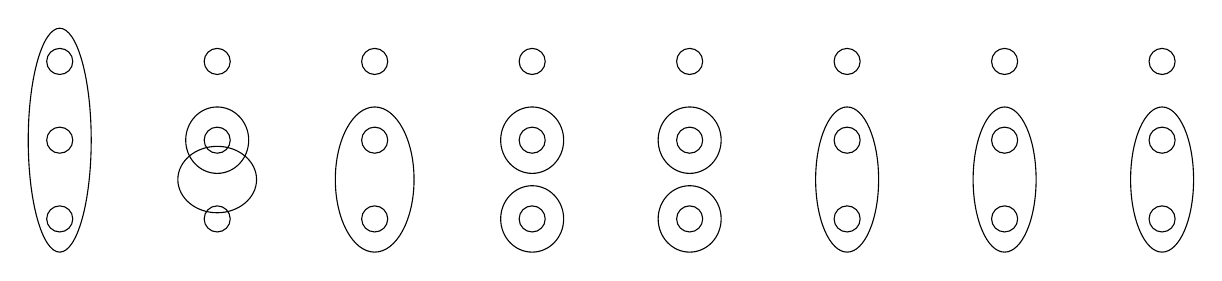
\begin{tikzpicture}[every node/.style={draw}] 
\centering
\node (l1) at (2,0) [circle] {};
\node (l2) at (4,0) [circle] {};
\node (l3) at (6,0) [circle] {};
\node (l4) at (8,0) [circle] {};
\node (l5) at (10,0) [circle] {};
\node (l6) at (12,0) [circle] {};
\node (l7) at (14,0) [circle] {};
\node (l8) at (16,0) [circle] {};

\node (m1) at (2,1) [circle] {};
\node (m2) at (4,1) [circle] {};
\node (m3) at (6,1) [circle] {};
\node (m4) at (8,1) [circle] {};
\node (m5) at (10,1) [circle] {};
\node (m6) at (12,1) [circle] {};
\node (m7) at (14,1) [circle] {};
\node (m8) at (16,1) [circle] {};

\node (k1) at (2,2) [circle] {};
\node (k2) at (4,2) [circle] {};
\node (k3) at (6,2) [circle] {};
\node (k4) at (8,2) [circle] {};
\node (k5) at (10,2) [circle] {};
\node (k6) at (12,2) [circle] {};
\node (k7) at (14,2) [circle] {};
\node (k8) at (16,2) [circle] {};

\draw let \p1=(l1), \p2=(k1), \n1={atan2(\y2-\y1,\x2-\x1)}, \n2={veclen(\y2-\y1,\x2-\x1)}
  in ($ (l1)!0.5!(k1) $) ellipse [x radius=\n2/2+12pt, y radius=0.4cm,rotate=0-\n1];
\draw let \p1=(l2), \p2=(l2), \n1={atan2(\y2-\y1,\x2-\x1)}, \n2={veclen(\y2-\y1,\x2-\x1)}
  in ($ (m2)!0.5!(m2) $) ellipse [x radius=\n2/2+12pt, y radius=0.4cm,rotate=0-\n1];
\draw let \p1=(l2), \p2=(l2), \n1={atan2(\y2-\y1,\x2-\x1)}, \n2={veclen(\y2-\y1,\x2-\x1)}
  in ($ (l2)!0.5!(m2) $) ellipse [x radius=\n2/2+12pt, y radius=0.5cm,rotate=0-\n1];
\draw let \p1=(l3), \p2=(m3), \n1={atan2(\y2-\y1,\x2-\x1)}, \n2={veclen(\y2-\y1,\x2-\x1)}
  in ($ (l3)!0.5!(m3) $) ellipse [x radius=\n2/2+12pt, y radius=0.5cm,rotate=0-\n1];
\draw let \p1=(l4), \p2=(l4), \n1={atan2(\y2-\y1,\x2-\x1)}, \n2={veclen(\y2-\y1,\x2-\x1)}
  in ($ (l4)!0.5!(l4) $) ellipse [x radius=\n2/2+12pt, y radius=0.4cm,rotate=0-\n1];
\draw let \p1=(m4), \p2=(m4), \n1={atan2(\y2-\y1,\x2-\x1)}, \n2={veclen(\y2-\y1,\x2-\x1)}
  in ($ (m4)!0.5!(m4) $) ellipse [x radius=\n2/2+12pt, y radius=0.4cm,rotate=0-\n1];
\draw let \p1=(l5), \p2=(l5), \n1={atan2(\y2-\y1,\x2-\x1)}, \n2={veclen(\y2-\y1,\x2-\x1)}
  in ($ (l5)!0.5!(l5) $) ellipse [x radius=\n2/2+12pt, y radius=0.4cm,rotate=0-\n1];
\draw let \p1=(m5), \p2=(m5), \n1={atan2(\y2-\y1,\x2-\x1)}, \n2={veclen(\y2-\y1,\x2-\x1)}
  in ($ (m5)!0.5!(m5) $) ellipse [x radius=\n2/2+12pt, y radius=0.4cm,rotate=0-\n1];
\draw let \p1=(l6), \p2=(m6), \n1={atan2(\y2-\y1,\x2-\x1)}, \n2={veclen(\y2-\y1,\x2-\x1)}
  in ($ (l6)!0.5!(m6) $) ellipse [x radius=\n2/2+12pt, y radius=0.4cm,rotate=0-\n1];
\draw let \p1=(l7), \p2=(m7), \n1={atan2(\y2-\y1,\x2-\x1)}, \n2={veclen(\y2-\y1,\x2-\x1)}
  in ($ (l7)!0.5!(m7) $) ellipse [x radius=\n2/2+12pt, y radius=0.4cm,rotate=0-\n1];
\draw let \p1=(l8), \p2=(m8), \n1={atan2(\y2-\y1,\x2-\x1)}, \n2={veclen(\y2-\y1,\x2-\x1)}
  in ($ (l8)!0.5!(m8) $) ellipse [x radius=\n2/2+12pt, y radius=0.4cm,rotate=0-\n1];
\end{tikzpicture}
 In the sequel we let $a_k:=\lambda ( kr_0 - (y-x))$
 denote the mean number of points in any lens,
 and note that the count $\sigma_k$ of $k$-hops is
 represented as the $U$-statistic of order $k-1$ 
$$ 
\sigma_k
= 
 \sum_{((x_1,l_1),\ldots , ((x_{k-1},l_{k-1}) ) \in \omega^d
   \atop (x_i,l_i)\not=(x_j,l_j), 1\leq i\not= j \leq d}
 f(x_1,l_1;\ldots ; x_{k-1},l_{k-1} )
$$
 where $u:X^d \mapsto \{0,1\}$ is the symmetrization in
 $d$ variables in $X$ of the indicator function  given by
 $$
 f(x_1,l_1;\ldots ; x_{k-1},l_{k-1})
 =
 \prod_{i=1}^d {\bf1}_{\{ x_i < x_{i+1} , l_i < l_{i+1}\}}
  =
  {\bf1}_{\{ l_1=1,\ldots , l_{k-1}={k-1}\}} 
  {\bf1}_{\{ x_1 < \cdots < x_{k-1} \}},
$$ 
 $((x_1,l_1),\ldots , (x_{k-1},l_{k-1}))\in X^{k-1}$. 
 
 \medskip  

 Proposition~\ref{djks1} shows that the moments of $\sigma_k$ 
 can be written using non-flat and non-crossing partition diagrams
 as 
\begin{equation} 
\nonumber 
 \E_m   [ ( \sigma_k)^n ] 
 = 
% \sum_{k=r}^{nr}  
 \sum_{
   \substack{
     \rho \in {\rm NC} [n\times r] 
     \\
     \rho \wedge \pi = \hat{0}
   }}
 \int_{X^{|\rho |}} 
 \prod_{k=1}^n u \big( z^\rho_k \big) 
 \sigma^{|\rho |} ( d \eufrak{z}_{|\rho |} ), 
\end{equation}
where ${\rm NC} [n\times r]$ is the set of partitions $\rho = \{\rho_1,\ldots , \rho_m\}$ 
 in $\Pi [n\times r]$ which are non-crossing in the sense that
 if $(k_1,l_1),(k_2,l_2)\in \rho_i$ and
 $(k'_1,l_1'),(k'_2,l_2') \in \rho_j$ belong to distinct  
 blocks $\rho_i,\rho_j$ of $\rho$ then
 we cannot have $1\leq l_1 < l_1' < l_2 < l_2' \leq n$. 


 Let $(N_t)_{t\in \real_+}$ denote
a Poisson process with time-dependent intensity $\lambda (t)$,
such that compensated Poisson process $M_t:=N_t-\int_0^t \lambda (s) ds$
is a square integrable martingale. 



From \eqref{ckn}, we have
\begin{eqnarray*} 
\frac{c_{k,n} (t,\ldots , t)}{ (c_{k,2}(t,\ldots , t) )^{n/2}}
 & = & 
\frac{c_{k,n}(t,\ldots , t)}{( \Var_m [ \sigma_k(t)] )^{n/2}} 
\\
 & \simeq & 
\frac{((2k-3)!)^{n/2}}{\lambda^{n(2k-3)/2}}
\frac{c_{k,n}(t,\ldots , t)}{ 2^{n(k-2)}
(kr-t)^{n(2k-3)/2}
}
\\
 & = & 
\frac{((2k-3)!)^{n/2}}{\lambda^{n(2k-3)/2}}
\frac{O ( (\lambda (kr-t))^{ 1 + (k-2)n })}{ 2^{n(k-2)}
(kr-t)^{n(2k-3)/2}
}
\\
 & = & O \big( \big( \sqrt{\lambda} \big)^{2-n} \big)
\end{eqnarray*} 
and therefore tends to zero as $\lambda$ tends to infinity,
$n\geq 2$.
 As a consequence of Theorem~1 in \cite{Janson1988}, 
the normalized $k$-hop count
$\widebar{\sigma}^{(m)}_k (t)$ 
converges in distribution to the standard normal
distribution as $\lambda$ tends to infinity. 


hence 
 \begin{eqnarray} 
   \nonumber
  | c_{3,n} ( t ) |  
   & \leq & 
  \sum_{l=1}^n
  \lambda^l \sum_{\pi_1\cup \cdots \cup \pi_l = \{1,\ldots , n\} }
  \int_{[0,t]^l} 
  \left|
  c^{|\pi|}_{2,l} ( u_1,\ldots , u_l) 
  \right|
  du_1\cdots du_l
    \\
  \nonumber 
  & = & 
  \sum_{l=1}^n
  l! \lambda^l 
  \sum_{\pi_1\cup \cdots \cup \pi_l = \{1,\ldots , n\} }
  \int_0^t \int_0^{u_l} \cdots \int_0^{u_2} 
  | c^\pi_{2,l} ( u_1,\ldots , u_l ) |
  du_1\cdots du_l, 
\end{eqnarray} 
 hence
  $$
  c_{3,n} (
 t
 ,
 \ldots
 , 
 t ) 
 \leq (B_n)^3 (\lambda t)^{n+1}
, 
 $$
 and
$$
 c^{(l_1,\ldots , l_p)}_{3,n} (
 t
 ,
 \ldots
 , 
 t
 ) 
 = O ( \lambda^{2n+1-p} )
, 
$$
 where $n=l_1+\cdots + l_p$. 

 \begin{prop}
 In the case of $3$-hop counts, we have the bound
$$
 c_3 (X_1^{l_1},\ldots , X_p^{l_p}) \leq (2(\lambda + 1))^{n(k-1)+1-p} (B_n)^{k-2}. 
$$
  \end{prop}
  \begin{Proof}
 We have 
 \begin{eqnarray} 
   \nonumber
  | c_{k,n} ( t , \ldots , t ) |  
   & \leq & 
  \sum_{l=1}^n
  \lambda_k^l \sum_{\pi_1\cup \cdots \cup \pi_l = \{1,\ldots , n\} }
  \int_{[0,t]^l} 
  \left|
  c^\pi_{k-1,l} ( u_1,\ldots , u_l) 
  \right|
  du_1\cdots du_l
    \\
  \nonumber 
  & = & 
  \sum_{l=1}^n
  l! \lambda_k^l 
  \sum_{\pi_1\cup \cdots \cup \pi_l = \{1,\ldots , n\} }
  \int_0^t \int_0^{u_l} \cdots \int_0^{u_2} 
  | c^\pi_{k-1,l} ( u_1,\ldots , u_l ) |
  du_1\cdots du_l, 
\end{eqnarray} 
 $k\geq 2$, hence
  $$
  c_{k,n} (
 t
 ,
 \ldots
 , 
 t ) 
 \leq (B_n)^k (\lambda t)^{n(k-2)+1}
, 
 $$
 and
$$
 c^{(l_1,\ldots , l_p)}_{k,n} (
 t
 ,
 \ldots
 , 
 t
 ) 
 = O ( \lambda^{n(k-1)+1-p} )
, 
$$
 where $n=l_1+\cdots + l_p$. 
     We have 
 \begin{eqnarray} 
   \nonumber
     | c_{k,n} ( t , \ldots , t ) |  
     & \leq & 
  \sum_{l=1}^n
  \lambda_k^l \sum_{\pi_1\cup \cdots \cup \pi_l = \{1,\ldots , n\} }
  \int_{[0,t]^l} 
  | c^\pi_{k,l} ( u_1 , \ldots , u_l ) | 
  du_1\cdots du_l
    \\
  \nonumber 
  & = & 
  \sum_{l=1}^n
  l! \lambda_k^l 
  \sum_{\pi_1\cup \cdots \cup \pi_l = \{1,\ldots , n\} }
  \int_0^t \int_0^{u_l} \cdots \int_0^{u_2} 
  | c^\pi_{k,l} ( u_1, \ldots , u_l ) | 
  du_1\cdots du_l
    \\
  \nonumber 
  & = & 
  \sum_{l=1}^n
  l! \lambda_k^l 
  \sum_{\pi_1\cup \cdots \cup \pi_l = \{1,\ldots , n\} }
  (2(\lambda +1))^{n(k-2)+1-l}
    \\
  \nonumber 
  & \leq & 
  (2(\lambda_k +1))^{n(k-2)+1}
  (B_n)^{k-3}
  \sum_{l=1}^n
  S(n,l)
    \\
  \nonumber 
  & \leq & 
  (2(\lambda_k +1))^{n(k-2)+1}
(B_n)^{k-2}
    \\
  \nonumber 
  & \leq & 
  (2(\lambda_k +1))^{n(k-2)+1}
(n!)^{k-2}
  , 
\end{eqnarray} 
 $k\geq 2$, hence 
\begin{eqnarray*} 
\frac{c_{k,n} (t,\ldots , t)}{ (c_{k,2} (t,\ldots , t) )^{n/2}}
& \leq &
(2(\lambda_k +1))^{n(k-2)+1}
(B_n)^{k-2}
 2^{-n(k-2)}
\frac{((2k-3)!)^{n/2}}{\lambda^{n(2k-3)/2}}
\\
& = &
2
(\lambda_k +1)^{n(k-2)+1 - n(2k-3)/2}
(B_n)^{k-2}
((2k-3)!)^{n/2}
\\
& = &
2 (\lambda_k+1)^{(2-n)/2}
(B_n)^{k-2}
((2k-3)!)^{n/2}
\\
& = &
2 (\lambda_k+1)^{(2-n)/2}
\left(\frac{n}{\log n}\right)^{k-2}
((2k-3)!)^{n/2}
\end{eqnarray*} 
  \end{Proof}


  \begin{eqnarray} 
\nonumber
\lefteqn{
  c^{(n)}_k (s_1,\ldots ,  s_n )
  \leq 
 \lambda^n
 \int_0^{s_1} \cdots \int_0^{s_n}
  c^{(n)}_{k-1} (u_1,\ldots , u_n) du_1\cdots du_n 
}
\\
\nonumber
   &  &
  \hskip-0.2cm
  + \hskip-0.2cm 
  \sum_{1 \leq l \leq m < n} \hskip-0.2cm 
  (l-1)!
  (-1)^{l-1}
  \lambda^m
  \hskip-1cm
  \sum_{\pi_1\cup \cdots \cup \pi_l = \{1,\ldots , n\}
    \hskip-0.3cm
    \atop 
      {
        d_1+\cdots +d_l=m
        \atop 1\leq d_1 \leq |\pi_1|, \ldots , 1 \leq d_l \leq |\pi_l|
      }
  }
  \prod_{q=1}^l 
  \left(
  t^{d_q}
  ( \E_m  [ ( N_{\lambda t} )^{|\pi_q|} ] )^{k-2}
  S(|\pi_q|,d_q) 
  \right)
  \\
  \nonumber
  & = &  
  \lambda^n
  \int_0^{s_1} \cdots \int_0^{s_n}
  c^{(n)}_{k-1} (u_1,\ldots , u_n) du_1\cdots du_n 
   \\
   \nonumber
   &  &
  \hskip-0.2cm
  + \hskip-0.2cm 
  \sum_{1 \leq l \leq m < n} \hskip-0.2cm 
  (l-1)!
  (-1)^{l-1}
  (\lambda t)^m
  \hskip-1cm
  \sum_{\pi_1\cup \cdots \cup \pi_l = \{1,\ldots , n\}
    \hskip-0.3cm
    \atop 
      {
        d_1+\cdots +d_l=m
        \atop 1\leq d_1 \leq |\pi_1|, \ldots , 1 \leq d_l \leq |\pi_l|
      }
  }
  \prod_{q=1}^l 
  \left(
  ( \E_m  [ ( N_{\lambda t} )^{|\pi_q|} ] )^{k-2}
  S(|\pi_q|,d_q) 
  \right)
  \\
  \nonumber
  & = &  
  \lambda^n
  \int_0^{s_1} \cdots \int_0^{s_n}
  c^{(n)}_{k-1} (u_1,\ldots , u_n) du_1\cdots du_n 
   \\
   \nonumber
   &  &
  \hskip-0.2cm
  + \hskip-0.2cm 
  \sum_{1 \leq l \leq m < n} \hskip-0.2cm 
  (l-1)!
  (-1)^{l-1}
  (\lambda t)^m
  \hskip-1cm
  \sum_{\pi_1\cup \cdots \cup \pi_l = \{1,\ldots , n\}
    \hskip-0.3cm
    \atop 
      {
        d_1+\cdots +d_l=m
        \atop 1\leq d_1 \leq |\pi_1|, \ldots , 1 \leq d_l \leq |\pi_l|
      }
  }
  \prod_{q=1}^l 
  \left(
  ( ( \lambda t )^{|\pi_q|(k-2)}
    ( \E_m  [ ( N_1 )^{|\pi_q|} ] )^{k-2}
  )
  S(|\pi_q|,d_q) 
  \right)
  \\
  \nonumber
  & \leq &  
  \lambda^n
  \int_0^{s_1} \cdots \int_0^{s_n}
  c^{(n)}_{k-1} (u_1,\ldots , u_n) du_1\cdots du_n 
   \\
   \nonumber
   &  &
  \hskip-0.2cm
  + \hskip-0.2cm 
  \sum_{1 \leq l \leq m < n} \hskip-0.2cm 
  (l-1)!
  (-1)^{l-1}
  (\lambda t)^m
  \hskip-1cm
  \sum_{\pi_1\cup \cdots \cup \pi_l = \{1,\ldots , n\}
    \hskip-0.3cm
    \atop 
      {
        d_1+\cdots +d_l=m
        \atop 1\leq d_1 \leq |\pi_1|, \ldots , 1 \leq d_l \leq |\pi_l|
      }
  }
  \prod_{q=1}^l 
  \left(
  ( ( \lambda t )^{|\pi_q|(k-2)}
    ( \E_m  [ ( N_1 )^n ] )^{(k-2)}
  )
  S(|\pi_q|,d_q) 
  \right)
  \\
  \nonumber
  & \leq &  
  \lambda^n
  \int_0^{s_1} \cdots \int_0^{s_n}
  c^{(n)}_{k-1} (u_1,\ldots , u_n) du_1\cdots du_n 
   \\
   \nonumber
   &  &
  \hskip-0.2cm
  + \hskip-0.2cm 
  \sum_{1 \leq l \leq m < n} \hskip-0.2cm 
  (l-1)!
  (-1)^{l-1}
  (\lambda t)^m
  \hskip-1cm
  \sum_{\pi_1\cup \cdots \cup \pi_l = \{1,\ldots , n\}
    \hskip-0.3cm
    \atop 
      {
        d_1+\cdots +d_l=m
        \atop 1\leq d_1 \leq |\pi_1|, \ldots , 1 \leq d_l \leq |\pi_l|
      }
  }
  \prod_{q=1}^l 
  \left(
  ( ( \lambda t )^{|\pi_q|(k-2)}
    ( \E_m  [ ( N_1 )^n ] )^{(k-2)}
  )
  S(|\pi_q|,d_q) 
  \right). 
\end{eqnarray} 


 In particular,

\begin{eqnarray*} 
\lefteqn{
 c_{2,n} (t_1,\ldots ,  t_n )
 = 
 \sum_{l=1}^n
  (l-1)!
  (-1)^{l-1}
  \sum_{\pi_1\cup \cdots \cup \pi_l = \{1,\ldots , n\}}
  \prod_{j=1}^l 
  m_{2,n} (s_{\pi_j})
  }
  \\
 & = & 
 \sum_{l=1}^n
  (l-1)!
  (-1)^{l-1}
  \sum_{\pi_1\cup \cdots \cup \pi_l = \{1,\ldots , n\}}
  \prod_{j=1}^l 
  \left(
  \sum_{p_j=1}^{|\pi_j|} 
  \lambda_1^{p_j}
  \sum_{\eta_1\cup \cdots \cup \eta_{p_j} = \pi_j } 
  \int_{[0,s_{\min \eta_1}]}
  \cdots
  \int_{[0,s_{\min \eta_{p_j}}]}
  m_{1,|\pi_j|}^\eta (u_1,\ldots , u_{p_j} ) 
  du_1\cdots du_{p_j}
 \right) 
  \\
 & = & 
 \sum_{l=1}^n
  (l-1)!
  (-1)^{l-1}
  \sum_{\pi_1\cup \cdots \cup \pi_l = \{1,\ldots , n\}}
  \prod_{j=1}^l 
  \left(
  \sum_{p_j=1}^{|\pi_j|} 
  \lambda_1^{p_j}
  \sum_{\eta_1\cup \cdots \cup \eta_{p_j} = \pi_j } 
  s_{\min \eta_1}
  \cdots
  s_{\min \eta_{p_j}}
  \right)
  \\
   & = & t_1, 
\end{eqnarray*} 
 and 
\begin{eqnarray*} 
  \lefteqn{
  c_{3,n} (t_1,\ldots ,  t_n )
 = 
 \sum_{l=1}^n
  (l-1)!
  (-1)^{l-1}
  \sum_{\pi_1\cup \cdots \cup \pi_l = \{1,\ldots , n\}}
  \prod_{j=1}^l 
  m_{3,n} (s_{\pi_j})
  }
  \\
 & = & 
 \sum_{l=1}^n
  (l-1)!
  (-1)^{l-1}
  \sum_{\pi_1\cup \cdots \cup \pi_l = \{1,\ldots , n\}}
  \prod_{j=1}^l 
  \left(
  \sum_{p_j=1}^{|\pi_j|} 
  \lambda_2^{p_j}
  \sum_{\eta_1\cup \cdots \cup \eta_{p_j} = \pi_j } 
  \int_{[0,s_{\min \eta_1}]}
  \cdots
  \int_{[0,s_{\min \eta_{p_j}}]}
  m_{2,|\pi_j|}^\eta (u_1,\ldots , u_{p_j} ) 
  du_1\cdots du_{p_j}
 \right), 
\end{eqnarray*} 
hence
\begin{eqnarray*} 
  \lefteqn{
   c_{3,n} (t,\ldots ,  t )
  }
  \\
 & = & 
 \sum_{l=1}^n
  (l-1)!
  (-1)^{l-1}
  \sum_{\pi_1\cup \cdots \cup \pi_l = \{1,\ldots , n\}}
  \prod_{j=1}^l 
  \left(
  \sum_{p_j=1}^{|\pi_j|} 
  \lambda_2^{p_j}
  \sum_{\eta_1\cup \cdots \cup \eta_{p_j} = \pi_j } 
  \int_{[0,t]}
  \cdots
  \int_{[0,t]} 
  m_{2,|\pi_j|}^\eta (u_1,\ldots , u_{p_j} ) 
  du_1\cdots du_{p_j}
 \right) 
 .
\end{eqnarray*} 
and
\begin{eqnarray*} 
  \\
& = &  
  \sum_{l=1}^2
  \sum_{\pi_1\cup \cdots \cup \pi_l = \{1,\ldots , 2\}}
  \int_{[0,s_{\min \pi_1}]}
  \cdots
  \int_{[0,s_{\min \pi_l}]}
  m_{k,2}^{|\pi|} (u_1,\ldots , u_l ) 
  \lambda_k (du_1) \cdots \lambda_k (du_l). 
\end{eqnarray*}


In the case of third order standard cumulants, we have
\begin{align*}
&
 \kappa_3 \big( Z^{(k+1)}_t \big)^3 
 =
 \E\big[ \big( Z^{(k+1)}_t \big)^3 \big] 
 - 3 \E_m  \big[ \big( Z^{(k+1)}_t \big)^2 \big]
 \E_m  \big[ Z^{(k+1)}_t \big]
 + 2 \big(  \E_m  \big[ Z^{(k+1)}_t \big] \big)^2 
\\
 & = 
  \int_0^t
  \E_m  \big[ \big( Z^{(k)}_{s_1} \big)^3 \big] 
  ds_1
  +
  3 \int_0^t
  \int_0^t
  \E_m  \big[ \big( Z^{(k)}_{s_1} \big)^2 Z^{(k)}_{s_3} \big]
  ds_1 ds_3 
 - 3   \int_0^t
\E_m  \big[ \big( Z^{(k)}_{s_1} \big)^2 \big]
ds_1 
\int_0^t
\E_m  \big[ Z^{(k)}_{s_1} \big]
ds_1
\\
 & 
-3 \int_0^t \int_0^t
\E_m  \big[ Z^{(k)}_{s_1} Z^{(k)}_{s_2} \big]
ds_1 ds_2 
\int_0^t
\E_m  \big[ Z^{(k)}_{s_1} \big]
ds_1 
\\
  & 
  + 
  \int_0^t
  \int_0^t
  \int_0^t
  \E_m  \big[ Z^{(k)}_{s_1} Z^{(k)}_{s_2} Z^{(k)}_{s_3} \big]
  ds_1ds_2ds_3
   + 2 \left( \int_0^t
\E_m  \big[ Z^{(k)}_{s_1} \big]
ds_1 \right)^3. 
\end{align*}


We have
  $$
  m_{3,n}(t,\ldots , t)
=
  \sum_{l=1}^n
  \sum_{\pi_1\cup \cdots \cup \pi_l = \{1,\ldots , n\}}
  \int_0^t
  \cdots
  \int_0^t
  m_{2,n}^{|\pi|} (u_1,\ldots , u_l ) 
  \lambda_2 (du_1) \cdots \lambda_2 (du_l)
. 
  $$
  When $k=3$, we have the joint moments 
\begin{eqnarray*}
  \E\big[ Z^{(3)}_{t_1} \cdots Z^{(3)}_{t_n} \big] & = &
  \sum_{l=1}^n \lambda_2^l 
  \sum_{\pi_1\cup \cdots \cup \pi_l = \{1,\ldots , n\}}
  \int_{\real_+^l} 
  \E_m  \left[ \prod_{j=1}^l
    \big(
    N_{s_j}^{(1)} 
    {\bf 1}_{[0,t_{\min \pi_j}]}(s_j)
    \big)^{|\pi_j|}
    \right] 
  ds_1\cdots ds_l
, 
\end{eqnarray*} 
 and the standard moments 
 $$
 \E\big[ \big(Z^{(3)}_t\big)^n\big]
   = 
  \sum_{k=1}^n
  \lambda_2^k
  \sum_{\pi_1\cup \cdots \cup \pi_k = \{1,\ldots , n\}}
  \int_0^t
  \cdots
  \int_0^t
  \E_m  \big[ \big( N_{s_1}^{(1)} \big)^{|\pi_1|}
  \cdots
  \big( N_{s_k}^{(1)} \big)^{|\pi_k|} \big] 
  ds_1\cdots ds_k. 
$$  

  \subsubsection*{Two-hop case}
We start with the two-hop case as an example
The $2$-hop count is given by 
$$ 
 \sigma_2 (t) = N_r - N_{t-r} \simeq N^{(1)}_{2r-t},
 \qquad t\in [r,2r], 
$$
 hence we have
\begin{eqnarray*} 
 \E_m  [ \sigma_2(2r-t_1)\cdots \sigma_2(2r-t_n) ]
 & : = & 
  \E_m  \big[ N^{(1)}_{t_1} \cdots N^{(1)}_{t_n} \big] 
  \\
  & = & 
  \sum_{l=1}^n \lambda_1^l
  \sum_{\eta_1\cup \cdots \cup \eta_l = \{1,\ldots , n\}}
 \int_{\real^l} 
\prod_{j=1}^l
\prod_{i=\eta_j} 
     {\bf 1}_{[0,t_i]}(u_j)
     du_1\cdots du_l
     \\
 & = & 
     \sum_{l=1}^n \lambda_1^l
     \sum_{\eta_1\cup \cdots \cup \eta_l = \{1,\ldots , n\}}
  \int_0^t
\cdots
  \int_0^t
\prod_{j=1}^l
     {\bf 1}_{[0, \min_{i\in \eta_j} t_i ]}(u_j)
     du_1\cdots du_l
     \\
 & = & 
     \sum_{l=1}^n \lambda_1^l
     \sum_{\eta_1\cup \cdots \cup \eta_l = \{1,\ldots , n\}}
\prod_{j=1}^l \min_{i\in \eta_j} t_i 
     \\
 & = & 
     \sum_{l=1}^n \lambda_1^l
     \sum_{\eta_1\cup \cdots \cup \eta_l = \{1,\ldots , n\}}
\prod_{j=1}^l t_{\min \eta_j}. 
\end{eqnarray*} 
 When $n=2$ the two partitions of $\{1,2\}$ can be listed as 
 $\pi_1 = \mlq 12\mrq$, and $\pi_1|\pi_2 = \mlq 1|2 \mrq$,
 which yields 
  $$
  \E_m  [N_{t_1}N_{t_2}] 
  =
  t_1 + t_1 t_2, 
  $$
 $0 \leq t_1\leq t_2$. 
 When $n=3$ there are $5$ partitions of $\{1,2,3\}$, which can be listed as 

 \medskip 

\noindent
$\pi_1 = \mlq 123\mrq$, 

 \medskip 

\noindent
$\pi_1 | \pi_2 = \mlq 12|3\mrq; \ \mlq 1|23\mrq; \ \mlq 13|2\mrq$,

\medskip 

\noindent
 $\pi_1| \pi_2 | \pi_3 = \mlq 1|2|3\mrq$,

\medskip 

 hence 
 $$
  \E_m  [N_{t_1}N_{t_2}N_{t_3}]
  =
  t_1t_2t_3 + 2 t_1 t_2 + t_1 t_3 + t_1, 
  $$
 $0\leq t_1\leq t_2\leq t_3$. For $n=4$ there are $15$ partitions of $\{1,2,3,4\}$, 
 that can be listed as 

\medskip 

\noindent
$\pi_1 = \mlq 1234\mrq$, % 1

\medskip 

\noindent
$ \pi_1 | \pi_2 = \mlq 12|34\mrq; \ 
\mlq 13|24\mrq; \ 
\mlq 14|23\mrq; \ 
\mlq 1|234\mrq; \ 
\mlq 2|134\mrq; \ 
\mlq 3|124\mrq; \ 
\mlq 4|123\mrq$, 

\medskip 

\noindent 
$\pi_1| \pi_2 | \pi_3 = 
\mlq 1|2|34\mrq; \ 
\mlq 1|3|24\mrq; \ 
\mlq 2|3|14\mrq; \ 
\mlq 2|4|13\mrq; \ 
\mlq 1|4|23\mrq; \ 
\mlq 3|4|12\mrq 
$,

\medskip 

\noindent
$ \pi_1 | \pi_2 | \pi_3 | \pi_4 = \mlq 1|2|3|4\mrq$, % 15

\medskip

hence we have 
  $$
  \E_m  [N_{t_1}N_{t_2}N_{t_3}N_{t_4}]
  =
  t_1t_2t_3t_4
  + 3 t_1t_2t_3 + 2 t_1t_2t_4 + t_1t_3t_4
  + 4 t_1 t_2 + 2 t_1 t_3 + t_1 t_4   
  + t_1, 
$$
 $0\leq t_1\leq t_2\leq t_3\leq t_4$.   
 In particular, we have $m_{1,n} = 1$, $n \geq 0$, and 
\begin{eqnarray*} 
\lefteqn{
  m_{2,n}(t_1,\ldots , t_n)}
  \\
   & = &  
  \sum_{l=1}^n
  \sum_{\pi_1\cup \cdots \cup \pi_l = \{1,\ldots , n\}}
  \int_{[0,t_{\min \pi_1}]}
  \cdots
  \int_{[0,t_{\min \pi_l}]}
  m_{1,n}^{|\pi|} (u_1,\ldots , u_l ) 
  \lambda_1 (du_1) \cdots \lambda_1 (du_l)
    \\
   & = &  
  \sum_{l=1}^n
  \sum_{\pi_1\cup \cdots \cup \pi_l = \{1,\ldots , n\}}
  \int_{[0,t_{\min \pi_1}]}
  \cdots
  \int_{[0,t_{\min \pi_l}]}
  \lambda_1 (du_1) \cdots \lambda_1 (du_l)
    \\
   & = &  
  \sum_{l=1}^n
  \lambda_1^l
  \sum_{\pi_1\cup \cdots \cup \pi_l = \{1,\ldots , n\}}
  t_{\min \pi_1}
  \cdots
  t_{\min \pi_l}, 
\end{eqnarray*} 
 and 
$$
  m_{3,n}(t,\ldots , t)
=
  \sum_{l=1}^n
  \sum_{\pi_1\cup \cdots \cup \pi_l = \{1,\ldots , n\}}
  \int_0^t
  \cdots
  \int_0^t
  m_{2,n}^{|\pi|} (u_1,\ldots , u_l ) 
  \lambda_2 (du_1) \cdots \lambda_2 (du_l)
. 
  $$
  When $k=3$, we have the joint moments 
\begin{eqnarray*}
  \E\big[ Z^{(3)}_{t_1} \cdots Z^{(3)}_{t_n} \big] & = &
  \sum_{l=1}^n \lambda_2^l 
  \sum_{\pi_1\cup \cdots \cup \pi_l = \{1,\ldots , n\}}
  \int_{\real_+^l} 
  \E_m  \left[ \prod_{j=1}^l
    \big(
    N_{s_j}^{(1)} 
    {\bf 1}_{[0,t_{\min \pi_j}]}(s_j)
    \big)^{|\pi_j|}
    \right] 
  ds_1\cdots ds_l
, 
\end{eqnarray*} 
 and the standard moments 
 $$
 \E\big[ \big(Z^{(3)}_t\big)^n\big]
   = 
  \sum_{k=1}^n
  \lambda_2^k
  \sum_{\pi_1\cup \cdots \cup \pi_k = \{1,\ldots , n\}}
  \int_0^t
  \cdots
  \int_0^t
  \E_m  \big[ \big( N_{s_1}^{(1)} \big)^{|\pi_1|}
  \cdots
  \big( N_{s_k}^{(1)} \big)^{|\pi_k|} \big] 
  ds_1\cdots ds_k. 
$$  
 We also have 
$$
  m_{k+1,1}(t_1)
  =
  \int_0^{t_1}
  m_{k,1}^{|\pi|} (u_1 ) 
  \lambda_k (du_1), 
$$
 which is solved as 
$$
  m_{k,1}(t_1)
=
\frac{t_1^{k-1}}{(k-1)!}.
$$
 We also have 
$$
  m_{k+1,2}(t_1, t_2)
=  
    \int_0^{t_1}
  m_{k,2} (u_1, u_1 ) 
  \lambda_k (du_1) 
 + 
   \int_0^{t_1} 
   \int_0^{t_2} 
  m_{k,2} (u_1, u_2 ) 
  \lambda_k (du_1) \lambda_k (du_2)
  , 
$$ 
 and 
\begin{eqnarray*} 
  m_{k+1,3}(t_1,t_2, t_3)
   & = &  
  \int_0^{t_1} 
  m_{k,3} (u_1, u_1,u_1 ) 
  \lambda_k (du_1) 
  \\
  & &
  + 
  \int_0^{\min (t_1,t_2)} 
  \int_0^{t_3} 
  m_{k,n} (u_1,u_1,u_3) 
  \lambda_k (du_1) \lambda_k (du_3)
  \\
  & &
  + 
  \int_0^{\min (t_1,t_3)} 
  \int_0^{t_2} 
  m_{k,n} (u_1,u_2,u_1) 
  \lambda_k (du_1) \lambda_k (du_2)
  \\
  & &
  + 
  \int_0^{t_1}
  \int_0^{\min (t_2,t_3)} 
  m_{k,n} (u_1,u_2,u_2) 
  \lambda_k (du_1) (du_2)
  \\
  & & + 
  \int_0^{t_1} 
  \int_0^{t_2} 
  \int_0^{t_3} 
  m_{k,n} (u_1,u_2,u_3) 
  \lambda_k (du_1) \lambda_k (du_2) \lambda_k (du_3). 
\end{eqnarray*} 


\begin{prop} 
\label{pr11} 
 Let $u_1,\ldots , u_p: \real_+ \times \Omega \longrightarrow \real$ 
 be random processes, $p\geq 1$. 
 For all $n_1, \ldots , n_p\geq 0$ and $n:=n_1+\cdots + n_p$, 
 we have 
\begin{eqnarray} 
\nonumber 
\lefteqn{ 
 \E_m  \left[ 
 \left( 
 \int_0^T u_1(t) dN_t 
 \right)^{n_1} 
 \cdots 
 \left( 
 \int_0^T u_p(t) dN_t 
 \right)^{n_p} 
 \right] 
} 
\\ 
\nonumber 
 & = & 
 \sum_{k=1}^n 
 ~ 
 \sum_{\pi_1 \cup \cdots \cup \pi_k = \{ 1, \ldots , n \} } 
 \E_m  \left[ 
 \int_{\real_+^k} 
% \epsilon_{t_1}^+ \cdots \epsilon_{t_k}^+ 
 \left( 
 \prod_{j=1}^k 
 \prod_{i=1}^p 
 u_i^{l^n_{i,j}} 
 (t_j , \xi ) 
 \right)  
 \lambda (dt_1) \cdots \lambda (dt_k) 
 \right] 
, 
\end{eqnarray} 
 where the sum runs over all partitions 
 $\pi_1,\ldots , \pi_k$ of $\{ 1 , \ldots , n \}$ 
 and the power $l^n_{i,j}$ is the cardinality  
$$ 
 l^n_{i,j} : = 
 | \pi_j \cap ( n_1+\cdots + n_{i-1},n_1+\cdots + n_i ]|,
 \qquad
 i=1,\ldots,k, \quad j=1,\ldots ,p. 
$$ 
\end{prop} 


\begin{prop} 
\label{djld} 
 Let $u : \real_+\times \Omega \longrightarrow \real$ be 
 a (measurable) process. For all $n\geq 1$ we have 
\begin{eqnarray} 
\label{fjds2} 
  \lefteqn{
    \E_m  \left[ 
 \left( \int_0^T u_t dN_t \right)^n 
 \right] 
  }
  \\
  \nonumber
  & = & 
 \sum_{k=1}^n 
 \sum_{ \pi_1\cup \cdots \cup \pi_k = \{1,\ldots , n\} } 
 \E_m  \left[ 
   \int_0^T \cdots \int_0^T
   % \epsilon^+_{t_1,\ldots , t_k}
   ( u^{|\pi_1|} (t_1 ) \cdots u^{|\pi_k|} (t_k ) ) 
   \lambda (dt_1) \cdots \lambda (dt_k) \right], 
\end{eqnarray} 
 where the sum runs over all partitions 
 $\rho$ of $\{ 1 , \ldots , n \}$ with cardinality $| \rho |$.
\end{prop} 



In the case of three-hops, we have
 $\E _m  [ \sigma_3 (3r-t) ] = t^2 \lambda_1 \lambda_2 / 2$ 
 and 
 $$
 \Var_m [ \sigma_3 (3r-t)]
 = 
 2 \frac{t^3}{3!}
 \left(
 \lambda_1\lambda_2^2
 + 
 \lambda_1^2\lambda_2
 \right)
 + t^2
 \frac{\lambda_1\lambda_2}{2!}, \quad t\in [0,1], 
$$   
% \subsubsection*{Second moment of $3$-process integrals} 
 and in the case of four-hops,
 $\E  [ \sigma_4 (4r-t) ] =  t^3 \lambda_1 \lambda_2 \lambda_3 / 3!$
 and 
\begin{eqnarray} 
\nonumber 
\Var [ \sigma_4 (4r-t)] & = & 
 \frac{t^5}{5!} \left( 6 
  \lambda_1^2\lambda_2^2\lambda_3
  + 4 
  \lambda_1^2\lambda_2\lambda_3^2
  + 6 
  \lambda_1\lambda_2^2\lambda_3^2
  \right)
  \\
  \nonumber
  & & 
  + 2\frac{t^4}{4!}
  \left(
 \lambda_1^2\lambda_2\lambda_3
 + 
 \lambda_1\lambda_2^2\lambda_3
 + 
 \lambda_1\lambda_2\lambda_3^2
 \right)
 + t^3
 \frac{\lambda_1\lambda_2\lambda_3}{3},
 \quad t\in [0,1]. 
\end{eqnarray} 


We also have
\begin{eqnarray*} 
 \kappa_4 ( \sigma_3(t) ) 
 & = & \E [ ( \sigma_3(t) -  \E  [ \sigma_3(t) ] )^4 ]
 -
 3 (\E [ ( \sigma_3(t) -  \E  [ \sigma_3(t) ] )^2 ])^2
\\
   & = &  
 \E  [ \sigma_3^4(t)] 
 - 4 \E  [ \sigma_3(t)] \E  [ \sigma_3^3(t) ]  
 - 3 ( \E  [ \sigma_3^2(t)])^2 
 + 12 \E  [ \sigma_3^2(t)] (\E  [ \sigma_3(t) ])^2   
 - 6 (\E  [ \sigma_3(t) ])^4
 \\
 & = &
 \frac{1}{2}t^2 + \frac{14}{3} t^3 + \frac{23}{2} t^4 + \frac{36}{5} t^5, 
\end{eqnarray*}  
 and 
$$
\kappa_5 ( \sigma_3(t) )
=
\frac{t^2}{2} + 10 t^3 + \frac{215}{4} t^4 + 86 t^5 + 41 t^6.
$$


In the case of three-hops we have 
$\E  [ \sigma_3 (3r-t)] = (\lambda t)^2/2$ and 
$$
\Var [ \sigma_3 (3r-t)]
= 
 \frac{2(\lambda t)^3}{3}
+ 
\frac{(\lambda t)^2}{2}.
$$   
% \subsubsection*{Second moment of $3$-process integrals} 
 In the case of four-hops, we find 
 $\E  [ \sigma_4 (4r-t)] = (\lambda t)^3/3!$ and 
 \begin{align} 
\nonumber 
 & 
\Var [ \sigma_4 (4r-t)] = 
 \frac{2(\lambda t)^5}{15}
 + \frac{(\lambda t)^4}{4}
 + \frac{(\lambda t)^3}{6} 
. 
\end{align} 
 In the case of five-hops, we find 
\begin{align} 
\nonumber 
 & 
\Var [ \sigma_5 (5r-t)] = 
\frac{(\lambda t)^4}{24} + \frac{(\lambda t)^5}{15} + \frac{(\lambda t)^6}{24} + \frac{4 (\lambda t)^7}{315}. % + \frac{a^8}{576}. 
\end{align} 


In the case of three-hops we have, using the command
 ${\rm mk}[\{s_1, s_2\}, \{\lambda_1, \lambda_2\}]$, $0< s_1<s_2$, 
 \begin{eqnarray*} 
 \E  [ \sigma_3 (3r-t_1) \sigma_3 (3r-t_2) ] 
 & = & 
 \frac{1}{2} \lambda_1 \lambda_2 t_1^2
 + \left( \frac{1}{3} \lambda_1^2 \lambda_2 
 - \frac{1}{6} \lambda_1 \lambda_2^2 \right)
 t_1^3
 \\
 & &
 + \frac{1}{2} \lambda_1 \lambda_2^2 t_1^2 t_2
 + \frac{1}{4} \lambda_1^2 \lambda_2^2 t_1^2 t_2^2,
 \end{eqnarray*} 
 $2r < t_2<t_1<3r$, and 
 In the case of four-hops, 
 the command
 ${\rm mk}[\{s_1, s_2\}, \{\lambda_1, \lambda_2, \lambda_3\}]$, $0< s_1<s_2$,
 yields 
 \begin{align*} 
 & 
     \E  [ \sigma_4 (4r-t_1) \sigma_4 (4r-t_2) ] 
 = 
\frac{1}{6} \lambda_1 \lambda_2 \lambda_3 t_1^3 + \frac{1}{12} \lambda_1^2 \lambda_2 \lambda_3 t_1^4 + \frac{1}{12} \lambda_1 \lambda_2^2 \lambda_3 t_1^4 - 
\frac{1}{12} \lambda_1 \lambda_2 \lambda_3^2 t_1^4 + \frac{1}{20} \lambda_1^2 \lambda_2^2 \lambda_3 t_1^5
      \\
& 
- 
 \frac{1}{20} \lambda_1^2 \lambda_2 \lambda_3^2 t_1^5 + \frac{1}{120} \lambda_1 \lambda_2^2 \lambda_3^2 t_1^5 + 
 \frac{1}{6} \lambda_1 \lambda_2 \lambda_3^2 t_1^3 t_2 + \frac{1}{12} \lambda_1^2 \lambda_2 \lambda_3^2 t_1^4 t_2 - 
 \frac{1}{24} \lambda_1 \lambda_2^2 \lambda_3^2 t_1^4 t_2
 \\
 &  
 + \frac{1}{12} \lambda_1 \lambda_2^2 \lambda_3^2 t_1^3 t_2^2 + 
 \frac{1}{36} \lambda_1^2 \lambda_2^2 \lambda_3^2 t_1^3 t_2^3
\end{align*} 
 $0<t_1<t_2<1$. 


\begin{NiceTabular}{c|c|c|c|c|} 
\cline{2-3}
 & 3-hops  & 4-hops    
\\ 
\cline{1-3} % \hline 
\multicolumn{1}{|c|}{First} & $\displaystyle \frac{\lambda^2}{2}$ & $\displaystyle \frac{\lambda^3}{6}$ 
\\ 
\cline{1-3} % \hline
\multicolumn{1}{|c|}{Second} & $\displaystyle \frac{\lambda^2}{2}+\frac{2\lambda^3}{3}$ & $\displaystyle \frac{\lambda^3}{6} + \frac{\lambda^4}{4} + \frac{2 \lambda^5}{15}$ % &  Time & Count  &  Time & Count   
\\ 
\cline{1-3} % \hline
\multicolumn{1}{|c|}{Third} & $\displaystyle \frac{\lambda^2}{2} + 2\lambda^3 + \frac{7\lambda^4}{4}$  & $\displaystyle \frac{\lambda^3}{6} + \frac{3 \lambda^4}{4} + \frac{5 \lambda^5}{4} + \frac{9 \lambda^6}{10} + \frac{69 \lambda^7}{280}$ 
\\ 
\cline{1-3}
\multicolumn{1}{|c|}{Fourth} & $\displaystyle
\frac{\lambda^2}{2}
+\frac{14 \lambda^3}{3}
+\frac{23 \lambda^4}{2}
+ \frac{36 \lambda^5}{5}
$  & $\displaystyle
\frac{\lambda^3}{6}+
\frac{7 \lambda^4}{4}
+
\frac{199 \lambda^5}{30}+
\frac{349 \lambda^6}{30}+
\frac{281 \lambda^7}{28}+
\frac{7223 \lambda^8}{1680}
+
\frac{2851 \lambda^9}{3780}
$ 
\\ 
\cline{1-3}
% \multicolumn{1}{|c|}{Fourth} & 0 & $\lambda$ & $\frac{\lambda^2}{2} + \frac{14\lambda^3}{3} + \frac{23 \lambda^4}{2} + \frac{36 \lambda^5}{5}$ & $\frac{\lambda^3}{6} + \frac{7 \lambda^4}{4} + \frac{199 \lambda^5}{30} + \frac{349 \lambda^6}{30} + \frac{281 \lambda^7}{28} + \frac{2403 \lambda^8}{560} + \frac{2119 \lambda^9}{2835} - \frac{7 \lambda^{10}}{5400} - \frac{\lambda^{11}}{14850240}$  
% \\ \cline{1-5}
\end{NiceTabular} 
\caption{Cumulants of 3-hop and 4-hop counts.} % in seconds.} 
\end{table} 

\vskip-0.3cm

\subsubsection*{Third joint moment of $3$-hops}
 We have
\begin{eqnarray*}
 \E\big[ Z^{(3)}_{t_1} Z^{(3)}_{t_2} Z^{(3)}_{t_3} ]
  & = & 
  -\frac{t_1^4}{4}+\frac{t_1^3 t_2^2}{12}+\frac{t_1^3 t_2}{2}+\frac{t_1^3 t_3^2}{12}+\frac{t_1^3 t_3}{2}+\frac{t_1^3}{2}+\frac{t_1^2 t_2^3}{12}+\frac{1}{8} t_1^2 t_2^2 t_3^2+\frac{1}{2} t_1^2 t_2^2 t_3+t_1^2 t_2^2
  \\
 &  & +\frac{1}{4} t_1^2 t_2 t_3^2+\frac{1}{2} t_1^2 t_2 t_3+t_1^2 t_2+\frac{t_1^2 t_3^2}{4}+\frac{t_1^2 t_3}{2}+\frac{t_1^2}{2}
\end{eqnarray*} 
 with 
$$ 
      \E[ (Z^{(3)}_t)^3 ]
  = 
  \frac{t^2}{2} 
  + 2t^3 +
  \frac{5}{2} t^4 + t^5
  + \frac{t^6}{8}. 
$$ 
 We have
\begin{eqnarray*}
 \E\big[ Z^{(3)}_{t_1} Z^{(3)}_{t_2} Z^{(3)}_{t_3} ]
  & = & 
  -\frac{t_1^4}{4}+\frac{t_1^3 t_2^2}{12}+\frac{t_1^3 t_2}{2}+\frac{t_1^3 t_3^2}{12}+\frac{t_1^3 t_3}{2}+\frac{t_1^3}{2}+\frac{t_1^2 t_2^3}{12}+\frac{1}{8} t_1^2 t_2^2 t_3^2+\frac{1}{2} t_1^2 t_2^2 t_3+t_1^2 t_2^2
  \\
 &  & +\frac{1}{4} t_1^2 t_2 t_3^2+\frac{1}{2} t_1^2 t_2 t_3+t_1^2 t_2+\frac{t_1^2 t_3^2}{4}+\frac{t_1^2 t_3}{2}+\frac{t_1^2}{2}
\end{eqnarray*} 
 with 
$$ 
      \E[ (Z^{(3)}_t)^3 ]
  = 
  \frac{t^2}{2} 
  + 2t^3 +
  \frac{5}{2} t^4 + t^5
  + \frac{t^6}{8}. 
$$ 
\subsubsection*{Fourth joint moment of $3$-hops}
  We have
\begin{align*}
&    \E\big[ Z^{(3)}_{t_1}Z^{(3)}_{t_2}Z^{(3)}_{t_3}Z^{(3)}_{t_4} \big]
   \\
  & = 
  \frac{1}{720} t_1^2 \left(-70 t_1^4+12 t_1^3 \left(5 t_2^2+30 t_2-18\right)-30 t_1^2 \left(2 t_2^3+10 t_2^2+3 t_3^2+8 t_3+3 t_4^2+8 t_4+60\right)
  \right.
  \\
  &
  +10 t_1 \left(-4 t_2^3+3 t_2^2 \left(t_3^2+8 t_3+t_4^2+8 t_4+26\right)+6 t_2 \left(3 t_3^2+14 t_3+3 t_4^2+14 t_4+46\right)
  \right.
  \\
   & 
  \left.
  +2 t_3^3+3 t_3^2 \left(t_4^2+8 t_4+20\right)+6 t_3 \left(3 t_4^2+14 t_4+32\right)+6 \left(3 t_4^2+18 t_4+14\right)\right)
  \\
  &
    +15 \left(-6 t_2^4+2 t_2^3 \left(t_3^2+8 t_3+t_4^2+8 t_4+10\right)
    \right.
    \\
  &
    +t_2^2 \left(2 t_3^3+3 t_3^2 \left(t_4^2+6 t_4+18\right)+12 t_3 \left(t_4^2+4 t_4+12\right)+24 \left(t_4^2+4 t_4+7\right)\right)
    \\
     & 
    +2 t_2 \left(2 t_3^3+3 t_3^2 \left(t_4^2+4 t_4+10\right)+6 t_3 \left(t_4^2+2 t_4+6\right)+12 \left(t_4^2+2 t_4+4\right)\right)
\\
     & 
    \left.
    \left.
        +2 \left(2 t_3^3+3 t_3^2 \left(t_4^2+4 t_4+8\right)+6 t_3 \left(t_4^2+2 t_4+4\right)+6 \left(t_4^2+2 t_4+2\right)\right)\right)\right)
        ,
        \end{align*} 
        and
        $$
        \E \big[ (Z^{(3)}_t)^4 \big]
        =
\frac{t^2}{2} + 14 \frac{t^3}{3} + 53 \frac{t^4}{4} + 66 \frac{t^5}{5}
  + 67 \frac{t^6}{12} + t^7 + \frac{t^8}{16}. 
% Wrong ? \frac{a^2}{2} + 7 a^3 + 25 a^4 + \frac{126}{5} a^5 + \frac{19}{2} a^6 + \frac{19}{14} a^7 + \frac{a^8}{16}, 
$$ 


  \subsubsection*{Second joint moment of $3$-hops}
 When $n=2$ the two partitions of $\{1,2\}$ can be listed as 
 $\pi_1 = \mlq 12\mrq$, and $\pi_1|\pi_2 = \mlq 1|2 \mrq$,
 which yields 
\begin{eqnarray*} 
\E \big[ Z^{(3)}_{t_1} Z^{(3)}_{t_2} \big] 
% & = & \E \left[ \left( \int_0^{3r-t} N^{(1)}_{s^-} dN^{(2)}_s \right)^2 \right] \\
% & = & \E \left[ \int_0^{3r-t} (N_s)^2 ds \right] + \E \left[ \int_0^{3r-t} \int_0^{3r-t} N_s N_u dsdu \right] \\
& = & 
 \lambda_1 \int_0^{t_1} \E \big[ \big(N_s^{(1)} \big)^2 \big] ds
 + 2 \lambda_1^2 \int_0^{t_1} \int_0^u \E \big[ N_s^{(1)} N_u^{(1)} \big] ds du 
 \\
  & & + \lambda_1^2 \int_0^{t_1} \int_{t2}^{t_1} \E \big[ N_s^{(1)} N_u^{(1)} \big] ds du 
% \\ & = & \int_0^{t_1} (s^2+s ) ds + 2 \int_0^{t_1} \int_0^u ( s + s u ) ds du \\ & & + \int_{t1}^{t_2} ( 1 + u ) \int_0^{t_1} s ds du 
% \\ & = & \frac{t_1^2}{2} + 2\frac{t_1^3}{3} + \frac{t_1^4}{4} + \frac{t_1^2}{2} \left( t_2 - t_1 + \frac{1}{2} \big( t_2^2 - t_1^2 \big) \right) 
\\
& = & 

\subsubsection*{Second joint moment of $3$-hops}
 When $n=2$ the two partitions of $\{1,2\}$ can be listed as 
 $\pi_1 = \mlq 12\mrq$, and $\pi_1|\pi_2 = \mlq 1|2 \mrq$,
 which yields 
\begin{eqnarray*} 
\E \big[ Z^{(3)}_{t_1} Z^{(3)}_{t_2} \big] 
% & = & \E \left[ \left( \int_0^{3r-t} N^{(1)}_{s^-} dN^{(2)}_s \right)^2 \right] \\
% & = & \E \left[ \int_0^{3r-t} (N_s)^2 ds \right] + \E \left[ \int_0^{3r-t} \int_0^{3r-t} N_s N_u dsdu \right] \\
& = & 
 \lambda_1 \int_0^{t_1} \E \big[ \big(N_s^{(1)} \big)^2 \big] ds
 + 2 \lambda_1^2 \int_0^{t_1} \int_0^u \E \big[ N_s^{(1)} N_u^{(1)} \big] ds du 
 \\
  & & + \lambda_1^2 \int_0^{t_1} \int_{t2}^{t_1} \E \big[ N_s^{(1)} N_u^{(1)} \big] ds du 
% \\ & = & \int_0^{t_1} (s^2+s ) ds + 2 \int_0^{t_1} \int_0^u ( s + s u ) ds du \\ & & + \int_{t1}^{t_2} ( 1 + u ) \int_0^{t_1} s ds du 
% \\ & = & \frac{t_1^2}{2} + 2\frac{t_1^3}{3} + \frac{t_1^4}{4} + \frac{t_1^2}{2} \left( t_2 - t_1 + \frac{1}{2} \big( t_2^2 - t_1^2 \big) \right) 
\\
& = & 
\frac{t_1^2}{2} 
+
\frac{t_1^3}{6}
+ \frac{1}{2} t_1^2 t_2
+ \frac{1}{4} t_1^2 t_2^2, 
\end{eqnarray*}
 and 
$$ 
\E \big[ \big(Z^{(3)}_t\big)^2 \big] 
 = 
\frac{t^2}{2} 
+
\frac{2t^3}{3}
+
\frac{t^4}{4}. 
$$



% \\ & = & \sum_{k=1}^n \frac{n!}{k!} \sum_{l_1+\cdots +l_k = n \atop l_1\geq 1, \ldots , l_k \geq 1} \int_0^t \cdots \int_0^t \frac{\E \big[ N_{s_1}^{l_1} \cdots N_{s_k}^{l_k} \big]}{l_1!\cdots l_k!} ds_1\cdots ds_k
 \\
  & = &
    \sum_{k=1}^n \lambda_2^k 
   \sum_{l_1+\cdots +l_k = n \atop l_1\geq 1, \ldots , l_k \geq 1} 
   \frac{n!}{l_1!\cdots l_k!}
   \int_0^t
  \int_0^{s_k}
  \cdots
  \int_0^{s_2} 
 \E \big[ \big( N_{s_1}^{(1)} \big)^{l_1}
  \cdots
  \big( N_{s_k}^{(1)} \big)^{l_k} \big] 
  ds_1\cdots ds_k,
  \end{eqnarray*} 
where the above sum is taken over (ordered) integer compositions
$(l_1,\ldots , l_k)$ of $n$. 


and
\begin{eqnarray*} 
\lefteqn{
  m_{k+1,n}(t_1,\ldots , t_n)}
  \\
   & = &  
  \sum_{l=1}^n
  \sum_{\pi_1\cup \cdots \cup \pi_l = \{1,\ldots , n\}}
  \int_{[0,t_{\min \pi_1}]}
  \cdots
  \int_{[0,t_{\min \pi_l}]}
  m_{k,l}^\pi  (u_1,\ldots , u_l ) 
  \lambda_k (du_1) \cdots \lambda_k (du_l), 
\end{eqnarray*} 


We have 
\begin{eqnarray*} 
  m_{k+1,3}(t_1,t_2, t_3)
   & = &  
  \int_0^{t_1} 
  m_{k,3} (u_1, u_1,u_1 ) 
  \lambda_k (du_1) 
  \\
  & &
  + 
  \int_0^{\min (t_1,t_2)} 
  \int_0^{t_3} 
  m_{k,3} (u_1,u_1,u_3) 
  \lambda_k (du_1) \lambda_k (du_3)
  \\
  & &
  + 
  \int_0^{\min (t_1,t_3)} 
  \int_0^{t_2} 
  m_{k,3} (u_1,u_2,u_1) 
  \lambda_k (du_1) \lambda_k (du_2)
  \\
  & &
  + 
  \int_0^{t_1}
  \int_0^{\min (t_2,t_3)} 
  m_{k,3} (u_1,u_2,u_2) 
  \lambda_k (du_1) (du_2)
  \\
  & & + 
  \int_0^{t_1} 
  \int_0^{t_2} 
  \int_0^{t_3} 
  m_{k,3} (u_1,u_2,u_3) 
  \lambda_k (du_1) \lambda_k (du_2) \lambda_k (du_3). 
\end{eqnarray*} 


$$
  m_{k+1,2}(s_1, s_2)
=  
    \int_0^{s_1}
  m_{k,2} (u_1, u_1 ) 
  \lambda_k (du_1) 
 + 
   \int_0^{s_1} 
   \int_0^{s_2} 
  m_{k,2} (u_1, u_2 ) 
  \lambda_k (du_1) \lambda_k (du_2)
  $$


  When $n=1$, the first moment in Proposition~\ref{djks1}
 yields the Georgii-Nguyen-Zessin identity 
\begin{equation} 
 \label{djksds} 
  \E  \left[ 
   \int_{X^r} f(z_1,\ldots , z_r;\omega ) \omega  (dz_1) \cdots
   \omega (dz_r) 
 \right] 
 = 
 \E  \left[ 
 \int_{X^r} 
 \epsilon^+_{\eufrak{z}_r} 
 f(z_1,\ldots ,z_r ;\omega )
 \mu^r ( d \eufrak{z}_r ) \right]. 
\end{equation} 
In the case of second moments, we find 
$$ 
  \E  \left[ 
    \left(
        \sum_{(z_1,\ldots , z_r ) \in \omega^r
   \atop z_i\not=z_j, 1\leq i\not= j \leq r}
     u(z_1,\ldots , z_r;\omega )
   \right)^2 
 \right] 
 = 
 \sum_{
   \substack{
     \rho \in \Pi [2\times r] 
     \\
     \rho \wedge \pi = \hat{0}
   }}
 \E  \left[ 
 \int_{X^{|\rho |}} 
 \epsilon^+_{\eufrak{z}_{|\rho |}} u \big( z^\rho_{\pi_1} \big) u \big( z^\rho_{\pi_2} \big) 
 \mu^{|\rho |} ( d \eufrak{z}_{|\rho |} ) \right]. 
$$ 
% \subsubsection*{Second moment of $2$-process integrals} 
In the case of second order $U$-statistics, we have 
\begin{align} 
\nonumber 
& \E  \left[ 
    \left(
              \sum_{(z_1,z_2 ) \in \omega^r
  z_1\not=z_2}
     u(z_1,z_2;\omega )
 \right)^2 
 \right] 
 = 
  \sum_{
   \substack{
     \rho \in \Pi [n\times 2] 
     \\
     \rho \wedge \pi = \hat{0}
   }}
 \E  \left[ 
 \int_{X^{|\rho |}} 
 \epsilon^+_{\eufrak{z}_{|\rho |}} \prod_{k=1}^n  u\big( z_{\zeta^\rho_{k,1}},z_{\zeta^\rho_{k,2}} \big)
 \mu^{|\rho |} ( d \eufrak{z}_{|\rho |} ) \right] 
\\
\nonumber
& = 
 \E  \left[ 
 \int_{X^4} 
 \epsilon^+_{\eufrak{z}_4} ( u(z_1,z_2 ) u(z_3,z_4 ) ) 
 \mu^4 ( d \eufrak{z}_4 ) \right]
\\
\nonumber
&  + 
 \E  \left[ 
 \int_{X^3} 
 \epsilon^+_{\eufrak{z}_3} ( u(z_1,z_2 )
 u(z_1,z_3 ) ) 
 \mu^3 ( d \eufrak{z}_3 ) \right]
+ 
 \E  \left[ 
 \int_{X^3} 
 \epsilon^+_{\eufrak{z}_3} ( u(z_2,z_1 )
 u(z_3,z_1 ) ) 
 \mu^3 ( d \eufrak{z}_3 ) \right]
\\
\nonumber
& 
+ 
 \E  \left[ 
 \int_{X^3} 
 \epsilon^+_{\eufrak{z}_3} ( u(z_1,z_2 )
 u(z_2,z_3 ) ) 
 \mu^3 ( d \eufrak{z}_3 ) \right]
+ 
 \E  \left[ 
 \int_{X^3} 
 \epsilon^+_{\eufrak{z}_3} ( u(z_2,z_1 )
 u(z_3,z_2 ) ) 
 \mu^3 ( d \eufrak{z}_3 ) \right]
 \\
\nonumber
& 
+ 
 \E  \left[ 
 \int_{X^2} 
 \epsilon^+_{\eufrak{z}_2} ( u(z_1,z_2 )
 u(z_1,z_2 ) ) 
 \mu^2 ( d \eufrak{z}_2 ) \right]
 +
 \E  \left[ 
 \int_{X^2} 
 \epsilon^+_{\eufrak{z}_2} ( u(z_1,z_2 )
 u(z_2,z_1 ) ) 
 \mu^2 ( d \eufrak{z}_2 ) \right]
. 
\end{align} 
% \subsubsection*{Second moment of $3$-process integrals} 
 In the case of third order $U$-statistics we find 
\begin{align} 
\nonumber 
 & 
  \E  \left[ 
    \left(
    \sum_{(z_1,z_2 , z_3 ) \in \omega^r
   \atop z_i\not=z_j, 1\leq i\not= j \leq 3}
     u(z_1,z_2 , z_3;\omega )
    \right)^2 
 \right] 
 = 
 \E  \left[ 
 \int_{X^6} 
 \epsilon^+_{\eufrak{z}_6} u(z_1,z_2,z_3 ) u(z_4,z_5,z_6 )
 \mu^{6} ( d \eufrak{z}_6 ) \right]
 \\
\nonumber
& \quad + 
\frac{1}{2}
\sum_{ \gamma : \{4,5,6\} \to \{ 1,5 , 6\} }
\E  \left[ 
 \int_{X^5} \epsilon^+_{\eufrak{z}_5} u ( z_1,z_2,z_3) u \big( z_{\gamma (4)} , z_{\gamma (5)} ,z_{\gamma (6)} \big) 
 \mu^5 ( d \eufrak{z}_5 ) \right]  
 \\
\nonumber
& \quad + 
\frac{1}{2}
\sum_{ \gamma : \{4,5,6\} \to \{ 2,5 , 6\} }
\E  \left[ 
 \int_{X^5} \epsilon^+_{\eufrak{z}_5} u ( z_1,z_2,z_3) u \big( z_{\gamma (4)} , z_{\gamma (5)} ,z_{\gamma (6)} \big) 
 \mu^5 ( d \eufrak{z}_5 ) \right]  
 \\
\nonumber
& \quad + 
\frac{1}{2}
\sum_{ \gamma : \{4,5,6\} \to \{ 3,5 , 6\} }
\E  \left[ 
 \int_{X^5} \epsilon^+_{\eufrak{z}_5} u ( z_1,z_2,z_3) u \big( z_{\gamma (4)} , z_{\gamma (5)} ,z_{\gamma (6)} \big) 
 \mu^5 ( d \eufrak{z}_5 ) \right]  
\\
\nonumber
& \quad + 
\sum_{
    \gamma : \{4,5,6\} \to \{1,2, 6\}
}
\E  \left[ 
 \int_{X^4} \epsilon^+_{\eufrak{z}_4} u ( z_1,z_2,z_3 ) u \big( z_{\gamma (4)} , z_{\gamma (5)} ,z_{\gamma (6)} \big) 
 \mu^4 ( d \eufrak{z}_4 ) \right]  
\\
\nonumber
& \quad + 
\sum_{
    \gamma : \{4,5,6\} \to \{1,3, 6\}
}
\E  \left[ 
 \int_{X^4} \epsilon^+_{\eufrak{z}_4} u ( z_1,z_2,z_3 ) u \big( z_{\gamma (4)} , z_{\gamma (5)} ,z_{\gamma (6)} \big) 
 \mu^4 ( d \eufrak{z}_4 ) \right]  
\\
\nonumber
& \quad + 
\sum_{
    \gamma : \{4,5,6\} \to \{2,3, 6\}
}
\E  \left[ 
 \int_{X^4} \epsilon^+_{\eufrak{z}_4} u ( z_1,z_2,z_3 ) u \big( z_{\gamma (4)} , z_{\gamma (5)} ,z_{\gamma (6)} \big) 
 \mu^4 ( d \eufrak{z}_4 ) \right]  
\\
\nonumber
& \quad + 
\sum_{
 \gamma : \{4,5,6\} \to \{1,2,3 \} 
}
\E  \left[ 
 \int_{X^3} \epsilon^+_{\eufrak{z}_3}z u ( z_1,z_2,z_3 ) u \big( z_{\gamma (4)} , z_{\gamma (5)} ,z_{\gamma (6)} \big) 
 \mu^3 ( d \eufrak{z}_3 ) \right]. 
\end{align} 
In the case of second order $U$-statistics, we have 
\begin{eqnarray} 
\nonumber 
 \E  [ \sigma_2^2(t) ] 
 & = & 
  \sum_{
   \substack{
     \rho \in \Pi [n\times 2] 
     \\
     \rho \wedge \pi = \hat{0}
   }}
 \int_{X^{|\rho |}} 
 \prod_{k=1}^n  u\big( z_{\zeta^\rho_{k,1}},z_{\zeta^\rho_{k,2}} \big)
 \mu^{|\rho |} ( d \eufrak{z}_{|\rho |} ) 
\\
\nonumber
& = & 
 \int_{X^4} 
 u(z_1,z_2 ) u(z_3,z_4 ) 
 \mu^4 ( d \eufrak{z}_4 ) 
 + 
 \int_{X^3} 
  u(z_1,z_2 )
 u(z_1,z_3 ) 
 \mu^3 ( d \eufrak{z}_3 ) 
 \\
\nonumber
& &
+ 
 \int_{X^3} 
 u(z_2,z_1 ) u(z_3,z_1 ) 
 \mu^3 ( d \eufrak{z}_3 ) 
+ 
 \int_{X^2} 
  u(z_1,z_2 ) u(z_1,z_2 ) 
 \mu^2 ( d \eufrak{z}_2 ) 
. 
\end{eqnarray} 
 In the case of third order $U$-statistics, we find 
\begin{align} 
\nonumber 
 & 
  \E  [ \sigma_3^2(t) ] 
 = 
\sum_{
  \substack{
    A \subset \{1,2,3\}
    \\
    \gamma : \{4,5,6\} \to A \cup \{ 4,\ldots , 6-|A|\}}
}
\frac{1}{(3-|A|)!}
\int_{X^5}
 u ( z_1,z_2,z_3 ) u \big( z_{\gamma (4)} , z_{\gamma (5)} ,z_{\gamma (6)} \big) 
 \mu^5 ( d \eufrak{z}_5  ) 
\\
\nonumber
& = 
 \int_{X^6} 
  u(z_1,z_2,z_3 ) u(z_4,z_5,z_6 )
 \mu^{6} ( d \eufrak{z}_6 ) 
 + 
 \int_{X^5}  u ( z_1,z_2,z_3) u (z_1,z_5,z_6) \mu^5 ( d \eufrak{z}_5 ) 
 \\
\nonumber
& \quad + 
 \int_{X^5}  u ( z_1,z_2,z_3) u ( z_5, z_2, z_6) \mu^5 ( d \eufrak{z}_5 ) 
 + 
 \int_{X^5} u ( z_1,z_2,z_3) u ( z_5, z_6, z_3) 
 \mu^5 ( d \eufrak{z}_5 ) 
\\
\nonumber
& \quad + 
 \int_{X^4} u ( z_1,z_2,z_3 ) u ( z_1,z_2,z_6)
 \mu^4 ( d \eufrak{z}_4 ) 
 + 
 \int_{X^4} u ( z_1,z_2,z_3 ) u (z_1,z_6,z_3)
 \mu^4 ( d \eufrak{z}_4 ) 
\\
\nonumber
& \quad + 
 \int_{X^4} u ( z_1,z_2,z_3 ) u (z_6,z_2,z_3) 
 \mu^4 ( d \eufrak{z}_4 ) 
 + 
 \int_{X^3} u^2 ( z_1,z_2,z_3 ) 
 \mu^3 ( d \eufrak{z}_3 ) 
 . 
\end{align} 


\\
   & = &  
 \sum_{l=1}^{n+1}
  (l-1)!
  (-1)^{l-1}
  \sum_{\pi_1\cup \cdots \cup \pi_l = \{1,\ldots , n+1\}}
  \prod_{j=1}^l 
  \E \Bigg[ \prod_{i\in \pi_j} X_i \Bigg]
  \\
     & &  
  +
  \sum_{\eta_1\cup \eta_2 = \{ 1, \ldots , n+1 \} \atop n \in \eta_1, \ n+1 \in \eta_2 }
  \sum_{l,l'=1}^n
  (l-1)!
  (-1)^{l-1}
  (l'-1)!
  (-1)^{l'-1}
  \sum_{\pi_1\cup \cdots \cup \pi_l = \eta_1 \cup \{n\}
    \atop
    \pi_1' \cup \cdots \cup \pi_{l'} = \eta_2 \cup \{ n+1 \}
  }
  \prod_{j=1}^l 
  \E \Bigg[ \prod_{i\in \pi_j} X_i \Bigg]
  \prod_{j'=1}^{l'} 
  \E \Bigg[ \prod_{i\in \pi_{j'}} X_i \Bigg]
  . 
\end{eqnarray*}
 By the relation
\begin{eqnarray*} 


  With this notation, we have
$$
 \widehat{m}_{k+1,n}^\eta (t_1,\ldots , t_n)
  = 
  \sum_{\eta \preceq \pi} 
  \int_{[0,t_{\min \pi_1}]}
  \cdots
  \int_{[0,t_{\min \pi_l}]}
  m_{k,n}^\pi (u_1,\ldots , u_l ) 
  \lambda_k (du_1) \cdots \lambda_k (du_l), 
$$ 
$0\leq t_1\leq \cdots \leq t_n$.
By the M\"obius inversion formula, see e.g. \S~2.5 of \cite{peccatitaqqu},
we also find the integrated moments 
$$
   \int_{[0,t_{\min \eta_1}]}
  \cdots
  \int_{[0,t_{\min \eta_l}]}
  m_{k,n}^{\eta} (u_1,\ldots , u_l ) 
  \lambda_k (du_1) \cdots \lambda_k (du_l)
= 
  \sum_{\eta \preceq \pi} 
  (-1)^{|\pi|-1}
  (|\pi|-1)!
 \widehat{m}_{k+1,n}^\pi (t_1,\ldots , t_n), 
$$ 
 and in particular
 $$ 
   \int_{[0,t_1]}
  \cdots
  \int_{[0,t_n]}
  m_{k,n} (u_1,\ldots , u_n ) 
  \lambda_k (du_1) \cdots \lambda_k (du_n)
=
  \sum_{l=1}^n
  (-1)^{l-1} (l-1)! \sum_{\pi_1\cup \cdots \cup \pi_l = \{1,\ldots , n\}}
\widehat{m}_{k+1,n}^\pi (t_1,\ldots , t_n)
  .
$$ 


From Proposition~\ref{djklfs2}, the
 variance of $\sigma_k (t)$ of $k$-hop paths is given by 
\begin{equation}
  \label{dfjkvar} 
  \Var [ \sigma_k (t)]
  =
  \sum_{l=1}^{k-1}
  \lambda_1^2\cdots \lambda_{k-1}^2
  \frac{(kr-t)^{2k-2-l}}{(2k-2-l)!} 
  \sum_{ j_0 + \cdots + j_l = k-1-l\atop j_0,\ldots , j_l\geq 0}
  \prod_{q=1}^l \frac{1}{\lambda_{j_0+\cdots + j_{q-1}+q}}
  \prod_{p=0}^l {2j_p \choose j_p}. 
\end{equation} 


with
\begin{eqnarray*} 
  \Var [ \sigma_k (t)]
  & \simeq & 
  \lambda_1^2\cdots \lambda_{k-1}^2
  \frac{(kr-t)^{2k-3}}{(2k-3)!} 
  \sum_{ j=0}^{k-2} 
  \frac{1}{\lambda_{j+1}}
  {2j \choose j}
  {2(k-2-j) \choose k-2-j}
  \\
   & = & 
  \lambda^{2k-3} 
  \frac{(kr-t)^{2k-3}}{(2k-3)!} 
  2^{2(k-2)}
%  \frac{\Gamma (k-1)}{(k-2)!}
\end{eqnarray*} 
 as $\lambda$ tends to infinity. 


 \begin{eqnarray*}
  \E[ Y_t^3 ]
  & = &
  \int_0^{3r-t}
  \E [ N_s^3 ]
  ds 
  +
  3 \int_0^{3r-t}
  \int_0^{s_2}
  \E [ N_{s_1}^2 N_{s_2}] 
  ds_1
  +
  3 \int_0^{3r-t}
  \int_0^{s_2}
  \E [ N_{s_1} N_{s_2}^2] 
  ds_1ds_2 
  \\
  & &
  + 
  \int_0^{3r-t}
  \int_0^{3r-t}
  \int_0^{3r-t}
  \E [ N_{s_1} N_{s_2} N_{s_3} ] 
  ds_1ds_2ds_3
   \\
  & = &
  \int_0^{3r-t}
  ( s^3 + 3 s^2 + s)
  ds 
  \\
  &  &
  +
  3 \int_0^{3r-t}
  \int_0^{s_2}
  (
  s_1^2 s_2 + s_1 s_2 + 2 s_1^2 + s_1 
  )
  ds_1ds_2 
  \\
  &  &
  +
  3 \int_0^{3r-t}
  \int_0^{s_2}
  (
  s_1 s_2^2 + 3 s_1 s_2 + s_1 
  )
  ds_1ds_2 
  \\
  & &
  + 
  6 \int_0^{3r-t}
  \int_0^{s_3} 
  \int_0^{s_2} 
  (
  s_1s_2s_3 + 2 s_1 s_2 + s_1 s_3 + s_1 
  )  
  ds_1ds_2ds_3
  \\
  & = &
  \int_0^{3r-t}
  ( s^3 + 3 s^2 + s)
  ds 
  \\
  &  &
  +
  3 \int_0^{3r-t}
  \int_0^{s_2}
  (
  s_1^2 s_2 + s_1 s_2^2 + 4 s_1 s_2 + 2 s_1^2 + 2 s_1 
  )
  ds_1ds_2 
  \\
  & &
  + 
  6 \int_0^{3r-t}
  \int_0^{s_3} 
  \int_0^{s_2} 
  (
  s_1s_2s_3 + 2 s_1 s_2 + s_1 s_3 + s_1 
  )  
  ds_1ds_2ds_3
  \\
  & = &
  \int_0^{3r-t}
  ( s^3 + 3 s^2 + s)
  ds 
  \\
  &  &
  +
  3 \int_0^{3r-t}
  (
  \frac{s_2^3}{3} s_2 + \frac{s_2^2}{2} s_2^2 + 4 \frac{s_2^2}{2} s_2 + 2 \frac{s_2^3}{3} +  s_2^2 
  )
  ds_2 
  \\
  & &
  + 
  6 \int_0^{3r-t}
  \int_0^{s_3} 
  (
  \frac{s_2^2}{2}s_2s_3 + 2 \frac{s_2^2}{2} s_2 + \frac{s_2^2}{2} s_3 + \frac{s_2^2}{2} 
  )  
  ds_2ds_3
  \\
  & = &
 \int_0^{3r-t}
  ( s^3 + 3 s^2 + s)
  ds 
  \\
  &  &
  +
  3 \int_0^{3r-t}
  (
  \frac{s_2^4}{3} + \frac{s_2^4}{2} + 4 \frac{s_2^3}{2} + 2 \frac{s_2^3}{3} + s_2^2 
  )
  ds_2 
  \\
  & &
  + 
  6 \int_0^{3r-t}
  \int_0^{s_3} 
  (
  \frac{s_2^3}{2}s_3 + 2 \frac{s_2^3}{2} + \frac{s_2^2}{2} s_3 + \frac{s_2^2}{2} 
  )  
  ds_2ds_3
  \\
  & = &
 \int_0^{3r-t}
  ( s^3 + 3 s^2 + s)
  ds 
  \\
  &  &
  +
  \int_0^{3r-t}
  (
  \frac{3s_2^4}{3} + \frac{3s_2^4}{2} + 4 \frac{3s_2^3}{2} + 2 \frac{3s_2^3}{3} + 3s_2^2 
  )
  ds_2 
  \\
  & &
  + 
  \int_0^{3r-t}
  \int_0^{s_3} 
  (
  \frac{6s_2^3}{2}s_3 + 2 \frac{6s_2^3}{2} + \frac{6s_2^2}{2} s_3 + \frac{6s_2^2}{2} 
  )  
  ds_2ds_3
  \\
  & = &
 \int_0^{3r-t}
  ( s^3 + 3 s^2 + s)
  ds 
  \\
  &  &
  +
  \int_0^{3r-t}
  (
  \frac{3s_2^4}{3} + \frac{3s_2^4}{2} + 4 \frac{3s_2^3}{2} + 2 \frac{3s_2^3}{3} + 3s_2^2 
  )
  ds_2 
  \\
  & &
  + 
  \int_0^{3r-t}
  \int_0^{s_3} 
  (
  \frac{6s_3^4}{8}s_3 + 2 \frac{6s_3^4}{8} + \frac{6s_3^3}{6} s_3 + \frac{6s_3^3}{6} 
  )  
  ds_2ds_3
  \\
  & = &
 \int_0^{3r-t}
  ( 3s_2^2 + 3 s^2 + s)
  ds 
  \\
  &  &
  +
  \int_0^{3r-t}
  (
  \frac{24s_2^4}{24} + \frac{36s_2^4}{24} + 2 \frac{18s_3^4}{24} + \frac{24s_3^4}{24}
  + \frac{6s_3^3}{6} + \frac{6s^3}{6} + 12 \frac{3s_2^3}{6} + 4 \frac{3s_2^3}{6} 
  )
  ds_2 
  \\
  & &
  + 
  \int_0^{3r-t}
  \int_0^{s_3} 
  (
  \frac{6s_3^5}{8} 
  )  
  ds_2ds_3
  \\
  & = &
 \int_0^{3r-t}
  ( 3s_2^2 + 3 s^2 + s)
  ds 
  +
  \int_0^{3r-t}
  (
  5s_2^4 + \frac{14}{3} s_2^3
  )
  ds_2 
  + 
  \int_0^{3r-t}
  \frac{6s_3^5}{8} 
  ds_3
  \\
  & = &
  \frac{s^2}{2} 
  + 2s_2^3 +
  \frac{14}{12} s_2^4 + s_2^5
  + \frac{s_3^6}{8} 
\end{eqnarray*} 

\begin{eqnarray*} 
\lefteqn{
 \kappa_{k,4} (t_1,t_2,t_3,t_4) 
 = 
 \sum_{l=1}^n
  (l-1)!
  (-1)^{l-1}
  \sum_{\pi_1\cup \cdots \cup \pi_l = \{1,\ldots , n\}}
  \prod_{j=1}^l 
  m_{k,|\pi_j|} (s_{\pi_j})
  }
  \\
& = &  
  m_{k+1,4} (t_1,t_2,t_3,t_4) 
  \\
  & & 
  - 
  m_{k+1,1} (t_1)m_{k+1,3} (t_2,t_3,t_4) 
  - 
  m_{k+1,1} (t_2)m_{k+1,3} (t_1,t_3,t_4) 
  - 
  m_{k+1,1} (t_3)m_{k+1,3} (t_1,t_2,t_4) 
  - 
  m_{k+1,1} (t_4)m_{k+1,3} (t_1,t_2,t_3) 
  \\
  & & 
  - 
  m_{k+1,2} (t_1,t_2)m_{k+1,2} (t_3,t_4) 
  - 
  m_{k+1,2} (t_1,t_3)m_{k+1,2} (t_2,t_4) 
  - 
  m_{k+1,2} (t_2,t_3)m_{k+1,2} (t_1,t_4) 
  \\
  & & 
  + 
  2m_{k+1,1} (t_1)m_{k+1,1} (t_2)m_{k+1,2} (t_3,t_4) 
  + 
  2m_{k+1,1} (t_1)m_{k+1,1} (t_3)m_{k+1,2} (t_2,t_4) 
  + 
  2m_{k+1,1} (t_1)m_{k+1,1} (t_4)m_{k+1,2} (t_2,t_3) 
  \\
  & &
  + 
  2m_{k+1,1} (t_2)m_{k+1,1} (t_3)m_{k+1,2} (t_1,t_4) 
    + 
  2m_{k+1,1} (t_2)m_{k+1,1} (t_4)m_{k+1,2} (t_1,t_3) 
    + 
  2m_{k+1,1} (t_3)m_{k+1,1} (t_4)m_{k+1,2} (t_1,t_2) 
  \\
  & &
  - 6 m_{k+1,1} (t_1)m_{k+1,1} (t_2)m_{k+1,1} (t_3)m_{k+1,1} (t_4)
\\
& = &  
  \int_0^{t_1} 
  m_{k,4} (u_1) 
  \lambda_k (du_1) 
  \\
  & &
  +
  \int_0^{t_1} 
  \int_0^{\min ( t_2,t_3,t_4)}
  m_{k,4} (u_1,u_2,u_2,u_2) 
  du_1du_2 
  +
  \int_0^{t_2} 
  \int_0^{\min ( t_1,t_3,t_4)}
  m_{k,4} (u_2,u_1,u_2,u_2) 
  du_1du_2 
  +
  \int_0^{t_3} 
  \int_0^{\min ( t_1,t_2,t_4)}
  m_{k,4} (u_2,u_2,u_1,u_2) 
  du_1du_2 
  +
  \int_0^{t_4} 
  \int_0^{\min ( t_1,t_2,t_3)}
  m_{k,4} (u_2,u_2,u_2,u_1) 
  du_1du_2 
 \\
  & &
  +
  \int_0^{\min (t_1,t_2)} 
  \int_0^{\min (t_3,t_4)} 
  m_{k,4} (u_1,u_1,u_2,u_2) 
  du_1du_2 
  +
  \int_0^{\min (t_1,t_3)} 
  \int_0^{\min (t_2,t_4)} 
  m_{k,4} (u_1,u_2,u_1,u_2) 
  du_1du_2 
  +
  \int_0^{\min (t_2,t_3)} 
  \int_0^{\min (t_1,t_4)} 
  m_{k,4} (u_1,u_2,u_2,u_1) 
  du_1du_2 
\\
  & &
  +
  \int_0^{t_1} 
  \int_0^{t_2}
  \int_0^{\min ( t_3,t_4)}
  m_{k,4} (u_1,u_2,u_3,u_3) 
  du_1du_2du_3
  +
  \int_0^{t_1} 
  \int_0^{t_3}
  \int_0^{\min ( t_2,t_4)}
  m_{k,4} (u_1,u_2,u_3,u_2) 
  du_1du_2du_3
  +
  \int_0^{t_1} 
  \int_0^{t_4}
  \int_0^{\min ( t_2,t_3)}
  m_{k,4} (u_1,u_2,u_2,u_3) 
  du_1du_2du_3
  \\
  & & 
  +
  \int_0^{t_2} 
  \int_0^{t_3}
  \int_0^{\min ( t_1,t_4)}
  m_{k,4} (u_1,u_2,u_3,u_1) 
  du_1du_2du_3
  +
  \int_0^{t_2} 
  \int_0^{t_4}
  \int_0^{\min ( t_1,t_3)}
  m_{k,4} (u_1,u_2,u_1,u_4) 
  du_1du_2du_3
  +
  \int_0^{t_3} 
  \int_0^{t_4}
  \int_0^{\min ( t_1,t_3)}
  m_{k,4} (u_1,u_2,u_3,u_3) 
  du_1du_2du_3
\\
  & & 
    +
  \int_0^{t_1} 
  \int_0^{t_2} 
  \int_0^{t_3} 
  \int_0^{t_4} 
  m_{k,4} (u_1,u_2,u_3,u_4) 
  du_1du_2du_3du_4
  \\
  & & 
  - 
  m_{k+1,1} (t_1)m_{k+1,3} (t_2,t_3,t_4) 
  - 
  m_{k+1,1} (t_2)m_{k+1,3} (t_1,t_3,t_4) 
  - 
  m_{k+1,1} (t_3)m_{k+1,3} (t_1,t_2,t_4) 
  - 
  m_{k+1,1} (t_4)m_{k+1,3} (t_1,t_2,t_3) 
  \\
  & & 
  - 
  m_{k+1,2} (t_1,t_2)m_{k+1,2} (t_3,t_4) 
  - 
  m_{k+1,2} (t_1,t_3)m_{k+1,2} (t_2,t_4) 
  - 
  m_{k+1,2} (t_2,t_3)m_{k+1,2} (t_1,t_4) 
  \\
  & & 
  + 
  2m_{k+1,1} (t_1)m_{k+1,1} (t_2)m_{k+1,2} (t_3,t_4) 
  + 
  2m_{k+1,1} (t_1)m_{k+1,1} (t_3)m_{k+1,2} (t_2,t_4) 
  + 
  2m_{k+1,1} (t_1)m_{k+1,1} (t_4)m_{k+1,2} (t_2,t_3) 
  \\
  & &
  + 
  2m_{k+1,1} (t_2)m_{k+1,1} (t_3)m_{k+1,2} (t_1,t_4) 
    + 
  2m_{k+1,1} (t_2)m_{k+1,1} (t_4)m_{k+1,2} (t_1,t_3) 
    + 
  2m_{k+1,1} (t_3)m_{k+1,1} (t_4)m_{k+1,2} (t_1,t_2) 
  \\
  & &
  - 6 m_{k+1,1} (t_1)m_{k+1,1} (t_2)m_{k+1,1} (t_3)m_{k+1,1} (t_4)
  \\
& = &  
  \int_0^{t_1} 
  m_{k,4} (u_1) 
  \lambda_k (du_1) 
  \\
  & &
  +
  \int_0^{t_1} 
  \int_0^{\min ( t_2,t_3,t_4)}
  m_{k,4} (u_1,u_2,u_2,u_2) 
  du_1du_2 
  +
  \int_0^{t_2} 
  \int_0^{\min ( t_1,t_3,t_4)}
  m_{k,4} (u_2,u_1,u_2,u_2) 
  du_1du_2 
  +
  \int_0^{t_3} 
  \int_0^{\min ( t_1,t_2,t_4)}
  m_{k,4} (u_2,u_2,u_1,u_2) 
  du_1du_2 
  +
  \int_0^{t_4} 
  \int_0^{\min ( t_1,t_2,t_3)}
  m_{k,4} (u_2,u_2,u_2,u_1) 
  du_1du_2 
 \\
  & &
  +
  \int_0^{\min (t_1,t_2)} 
  \int_0^{\min (t_3,t_4)} 
  m_{k,4} (u_1,u_1,u_2,u_2) 
  du_1du_2 
  +
  \int_0^{\min (t_1,t_3)} 
  \int_0^{\min (t_2,t_4)} 
  m_{k,4} (u_1,u_2,u_1,u_2) 
  du_1du_2 
  +
  \int_0^{\min (t_2,t_3)} 
  \int_0^{\min (t_1,t_4)} 
  m_{k,4} (u_1,u_2,u_2,u_1) 
  du_1du_2 
\\
  & &
  +
  \int_0^{t_1} 
  \int_0^{t_2}
  \int_0^{\min ( t_3,t_4)}
  m_{k,4} (u_1,u_2,u_3,u_3) 
  du_1du_2du_3
  +
  \int_0^{t_1} 
  \int_0^{t_3}
  \int_0^{\min ( t_2,t_4)}
  m_{k,4} (u_1,u_2,u_3,u_2) 
  du_1du_2du_3
  +
  \int_0^{t_1} 
  \int_0^{t_4}
  \int_0^{\min ( t_2,t_3)}
  m_{k,4} (u_1,u_2,u_2,u_3) 
  du_1du_2du_3
  \\
  & & 
  +
  \int_0^{t_2} 
  \int_0^{t_3}
  \int_0^{\min ( t_1,t_4)}
  m_{k,4} (u_1,u_2,u_3,u_1) 
  du_1du_2du_3
  +
  \int_0^{t_2} 
  \int_0^{t_4}
  \int_0^{\min ( t_1,t_3)}
  m_{k,4} (u_1,u_2,u_1,u_4) 
  du_1du_2du_3
  +
  \int_0^{t_3} 
  \int_0^{t_4}
  \int_0^{\min ( t_1,t_3)}
  m_{k,4} (u_1,u_2,u_3,u_3) 
  du_1du_2du_3
\\
  & & 
    +
  \int_0^{t_1} 
  \int_0^{t_2} 
  \int_0^{t_3} 
  \int_0^{t_4} 
  c_{k,4} (u_1,u_2,u_3,u_4) 
  du_1du_2du_3du_4
  \\
  & & 
  - 
  m_{k+1,1} (t_1)\left(
  \int_0^{\min (t_1,t_2)} 
  \int_0^{t_3} 
  m_{k,3} (u_1,u_1,u_3) 
  \lambda_k (du_1) \lambda_k (du_3)
  + 
  \int_0^{\min (t_1,t_3)} 
  \int_0^{t_2} 
  m_{k,3} (u_1,u_2,u_1) 
  \lambda_k (du_1) \lambda_k (du_2)
  + 
  \int_0^{t_1}
  \int_0^{\min (t_2,t_3)} 
  m_{k,3} (u_1,u_2,u_2) 
  \lambda_k (du_1) (du_2)
   + 
  \int_0^{t_1} 
  \int_0^{t_2} 
  \int_0^{t_3} 
  m_{k,3} (u_1,u_2,u_3) 
  \lambda_k (du_1) \lambda_k (du_2) \lambda_k (du_3) 
  \right) 
\\
 & & - 
  m_{k+1,1} (t_2)m_{k+1,3} (t_1,t_3,t_4) 
  - 
  m_{k+1,1} (t_3)m_{k+1,3} (t_1,t_2,t_4) 
  - 
  m_{k+1,1} (t_4)m_{k+1,3} (t_1,t_2,t_3) 
  \\
  & & 
  - 
  m_{k+1,2} (t_1,t_2)
  \left(
      \int_0^{t_2}
  m_{k,2} (u_1, u_1 ) 
  \lambda_k (du_1) 
\textcolor{red}{ + \int_0^{t_2} \int_0^{t_3} m_{k,2} (u_1, u_2 ) \lambda_k (du_1) \lambda_k (du_2)}
\right) 
  - 
  m_{k+1,2} (t_1,t_3)m_{k+1,2} (t_2,t_4) 
  - 
  m_{k+1,2} (t_2,t_3)m_{k+1,2} (t_1,t_4) 
  \\
  & & 
  + 
  2m_{k+1,1} (t_1)m_{k+1,1} (t_2)
    \left(
      \int_0^{t_3}
  m_{k,2} (u_1, u_1 ) 
  \lambda_k (du_1) 
% + \int_0^{t_3} \int_0^{t_4} m_{k,2} (u_1, u_2 ) \lambda_k (du_1) \lambda_k (du_2)
\right) 
  + 
  2m_{k+1,1} (t_1)m_{k+1,1} (t_3)m_{k+1,2} (t_2,t_4) 
  + 
  2m_{k+1,1} (t_1)m_{k+1,1} (t_4)m_{k+1,2} (t_2,t_3) 
  \\
  & &
  + 
  2m_{k+1,1} (t_2)m_{k+1,1} (t_3)m_{k+1,2} (t_1,t_4) 
    + 
  2m_{k+1,1} (t_2)m_{k+1,1} (t_4)m_{k+1,2} (t_1,t_3) 
    + 
  2m_{k+1,1} (t_3)m_{k+1,1} (t_4)m_{k+1,2} (t_1,t_2) 
 \\
& = &  
  \int_0^{t_1} 
  m_{k,4} (u_1) 
  \lambda_k (du_1) 
  \\
  & &
  +
  \int_0^{t_1} 
  \int_0^{\min ( t_2,t_3,t_4)}
  m_{k,4} (u_1,u_2,u_2,u_2) 
  du_1du_2 
  +
  \int_0^{t_2} 
  \int_0^{\min ( t_1,t_3,t_4)}
  m_{k,4} (u_2,u_1,u_2,u_2) 
  du_1du_2 
  +
  \int_0^{t_3} 
  \int_0^{\min ( t_1,t_2,t_4)}
  m_{k,4} (u_2,u_2,u_1,u_2) 
  du_1du_2 
  +
  \int_0^{t_4} 
  \int_0^{\min ( t_1,t_2,t_3)}
  m_{k,4} (u_2,u_2,u_2,u_1) 
  du_1du_2 
 \\
  & &
  +
  \int_0^{\min (t_1,t_2)} 
  \int_0^{\min (t_3,t_4)} 
  m_{k,4} (u_1,u_1,u_2,u_2) 
  du_1du_2 
  +
  \int_0^{\min (t_1,t_3)} 
  \int_0^{\min (t_2,t_4)} 
  m_{k,4} (u_1,u_2,u_1,u_2) 
  du_1du_2 
  +
  \int_0^{\min (t_2,t_3)} 
  \int_0^{\min (t_1,t_4)} 
  m_{k,4} (u_1,u_2,u_2,u_1) 
  du_1du_2 
\\
  & &
  +
  \int_0^{t_1} 
  \int_0^{t_2}
  \int_0^{\min ( t_3,t_4)}
  c_{k,4} (u_1,u_2,u_3,u_3) 
  du_1du_2du_3
  +
  \int_0^{t_1} 
  \int_0^{t_3}
  \int_0^{\min ( t_2,t_4)}
  c_{k,4} (u_1,u_2,u_3,u_2) 
  du_1du_2du_3
  +
  \int_0^{t_1} 
  \int_0^{t_4}
  \int_0^{\min ( t_2,t_3)}
  c_{k,4} (u_1,u_2,u_2,u_3) 
  du_1du_2du_3
  \\
  & & 
  +
  \int_0^{t_2} 
  \int_0^{t_3}
  \int_0^{\min ( t_1,t_4)}
  c_{k,4} (u_1,u_2,u_3,u_1) 
  du_1du_2du_3
  +
  \int_0^{t_2} 
  \int_0^{t_4}
  \int_0^{\min ( t_1,t_3)}
  m_{k,4} (u_1,u_2,u_1,u_4) 
  du_1du_2du_3
  +
  \int_0^{t_3} 
  \int_0^{t_4}
  \int_0^{\min ( t_1,t_3)}
  c_{k,4} (u_1,u_2,u_3,u_3) 
  du_1du_2du_3
\\
  & & 
    +
  \int_0^{t_1} 
  \int_0^{t_2} 
  \int_0^{t_3} 
  \int_0^{t_4} 
  c_{k,4} (u_1,u_2,u_3,u_4) 
  du_1du_2du_3du_4
  \\
  & & 
  - 
  m_{k+1,1} (t_1)\left(
  \int_0^{t_1} 
    m_{k,3} (u_1,u_1,u_1) 
  \lambda_k (du_1) 
  \right) 
\\
 & & - 
  m_{k+1,1} (t_2)m_{k+1,3} (t_1,t_3,t_4) 
  - 
  m_{k+1,1} (t_3)m_{k+1,3} (t_1,t_2,t_4) 
  - 
  m_{k+1,1} (t_4)m_{k+1,3} (t_1,t_2,t_3) 
  \\
  & & 
  - 
  m_{k+1,2} (t_1,t_2)
  \left(
      \int_0^{t_2}
  m_{k,2} (u_1, u_1 ) 
  \lambda_k (du_1) 
\textcolor{red}{ + \int_0^{t_2} \int_0^{t_3} m_{k,2} (u_1, u_2 ) \lambda_k (du_1) \lambda_k (du_2)}
\right) 
  - 
  m_{k+1,2} (t_1,t_3)m_{k+1,2} (t_2,t_4) 
  - 
  m_{k+1,2} (t_2,t_3)m_{k+1,2} (t_1,t_4) 
 \\
& = &  
  \int_0^{t_1} 
  m_{k,4} (u_1) 
  \lambda_k (du_1) 
  \\
  & &
  +
  \int_0^{t_1} 
  \int_0^{\min ( t_2,t_3,t_4)}
  c_{k,4} (u_1,u_2,u_2,u_2) 
  du_1du_2 
  +
  \int_0^{t_2} 
  \int_0^{\min ( t_1,t_3,t_4)}
  m_{k,4} (u_2,u_1,u_2,u_2) 
  du_1du_2 
  +
  \int_0^{t_3} 
  \int_0^{\min ( t_1,t_2,t_4)}
  c_{k,4} (u_2,u_2,u_1,u_2) 
  du_1du_2 
  +
  \int_0^{t_4} 
  \int_0^{\min ( t_1,t_2,t_3)}
  c_{k,4} (u_2,u_2,u_2,u_1) 
  du_1du_2 
 \\
  & &
  +
  \int_0^{\min (t_1,t_2)} 
  \int_0^{\min (t_3,t_4)} 
  c_{k,4} (u_1,u_1,u_2,u_2) 
  du_1du_2 
  +
  \int_0^{\min (t_1,t_3)} 
  \int_0^{\min (t_2,t_4)} 
  c_{k,4} (u_1,u_2,u_1,u_2) 
  du_1du_2 
  +
  \int_0^{\min (t_2,t_3)} 
  \int_0^{\min (t_1,t_4)} 
  c_{k,4} (u_1,u_2,u_2,u_1) 
  du_1du_2 
\\
  & &
  +
  \int_0^{t_1} 
  \int_0^{t_2}
  \int_0^{\min ( t_3,t_4)}
  c_{k,4} (u_1,u_2,u_3,u_3) 
  du_1du_2du_3
  +
  \int_0^{t_1} 
  \int_0^{t_3}
  \int_0^{\min ( t_2,t_4)}
  c_{k,4} (u_1,u_2,u_3,u_2) 
  du_1du_2du_3
  +
  \int_0^{t_1} 
  \int_0^{t_4}
  \int_0^{\min ( t_2,t_3)}
  c_{k,4} (u_1,u_2,u_2,u_3) 
  du_1du_2du_3
  \\
  & & 
  +
  \int_0^{t_2} 
  \int_0^{t_3}
  \int_0^{\min ( t_1,t_4)}
  c_{k,4} (u_1,u_2,u_3,u_1) 
  du_1du_2du_3
  +
  \int_0^{t_2} 
  \int_0^{t_4}
  \int_0^{\min ( t_1,t_3)}
  m_{k,4} (u_1,u_2,u_1,u_4) 
  du_1du_2du_3
  +
  \int_0^{t_3} 
  \int_0^{t_4}
  \int_0^{\min ( t_1,t_3)}
  c_{k,4} (u_1,u_2,u_3,u_3) 
  du_1du_2du_3
\\
  & & 
    +
  \int_0^{t_1} 
  \int_0^{t_2} 
  \int_0^{t_3} 
  \int_0^{t_4} 
  c_{k,4} (u_1,u_2,u_3,u_4) 
  du_1du_2du_3du_4
  \\
  & & 
  - 
   \left(
   \textcolor{red}{ \int_0^{t_2} \int_0^{t_3} m_{k,2} (u_1, u_2 ) \lambda_k (du_1) \lambda_k (du_2)}
\right) 
 \left(
   \textcolor{red}{ \int_0^{t_2} \int_0^{t_3} m_{k,2} (u_1, u_2 ) \lambda_k (du_1) \lambda_k (du_2)}
\right) 
  - 
  m_{k+1,2} (t_1,t_3)m_{k+1,2} (t_2,t_4) 
  - 
  m_{k+1,2} (t_2,t_3)m_{k+1,2} (t_1,t_4) 
  \\
  & & + 12
  \\
  & & - 6
  , 
\end{eqnarray*} 



\begin{Proof}
 We have 
\begin{eqnarray} 
   \nonumber
   \lefteqn{
     \kappa_{k+1,n} \big(
 Z^{(k+1)}_t
 ,
 \ldots
 , 
 Z^{(k+1)}_t
 \big) 
 }
   \\
  \nonumber 
  & = & 
 \sum_{l=1}^n
  (l-1)!
  (-1)^{l-1}
  \sum_{\eta_1\cup \cdots \cup \eta_l = \{1,\ldots , n\}}
  \prod_{j=1}^l 
  \E \Bigg[ \prod_{i\in \eta_j} Z_t^{(k+1)} \Bigg]. 
  \\
  & = &
  \sum_{l=1}^n
  \lambda_{k+1}^l \sum_{\pi_1\cup \cdots \cup \pi_l = \{1,\ldots , n\} }
  \int_{\prod_{i=1}^l [0,t]}
  \kappa_{k,l}
  \Big( \left( \big( Z^{(k)}_{u_i} \big)^{|\pi_i|} \right)_{i=1,\ldots , l} \Big)
  du_1\cdots du_l
  , 
\end{eqnarray} 


$$ 
 \kappa (Z_1^{l_1},\ldots , Z_n^{l_n}) 
 = 
 \sum_{l=1}^n
  (l-1)!
  (-1)^{l-1}
  \sum_{\eta_1\cup \cdots \cup \eta_l = \{1,\ldots , n\}}
  \prod_{j=1}^l 
  \E \Bigg[ \prod_{i\in \eta_j} Z_i^{l_i} \Bigg]. 
$$
  and
$$ 
 \E \big[ Z_1^{l_1}\cdots Z_n^{l_n} \big] 
 = 
 \sum_{l=1}^n
 \sum_{\eta_1\cup \cdots \cup \eta_l = \{1,\ldots , n\}}
 \prod_{j=1}^l 
 \kappa \big(\big( Z_i^{l_i} \big)_{i\in \pi_j} \big) 
$$
$$
m_{k+1,n}(s_1,\ldots , s_n)
=
  \sum_{l=1}^n
  \sum_{\pi_1\cup \cdots \cup \pi_l = \{1,\ldots , n\}}
  \int_{[0,s_{\min \pi_1}]}
  \cdots
  \int_{[0,s_{\min \pi_l}]}
  m_{k,n}^\pi  (u_1,\ldots , u_l ) 
  \lambda_k (du_1) \cdots \lambda_k (du_l), 
  $$
 By the joint cumulant inversion relation, we have  
\begin{eqnarray*} 
  \lefteqn{
    \kappa_{k+1,n} (t,\ldots ,  t )
  = 
 \sum_{l=1}^n
  (l-1)!
  (-1)^{l-1}
  \sum_{\pi_1\cup \cdots \cup \pi_l = \{1,\ldots , n\}}
  \prod_{j=1}^l 
  \widehat{m}_{k+1,|\pi_j|} (t,\ldots , t) 
  }
\\
 & = & 
  \sum_{l=1}^n
  (l-1)!
  (-1)^{l-1}
  \sum_{\pi_1\cup \cdots \cup \pi_l = \{1,\ldots , n\}}
  \prod_{j=1}^l 
  \sum_{\eta^{(j)} \preceq \pi_j } 
  \int_0^t 
  \cdots
  \int_0^t 
  m_{k,n}^{\eta^{(j)}} (u_1,\ldots , u_p ) 
  \lambda_k (du_1) \cdots \lambda_k (du_p), 
\\
 & = & 
  \sum_{l=1}^n
  (l-1)!
  (-1)^{l-1}
  \sum_{\pi_1\cup \cdots \cup \pi_l = \{1,\ldots , n\}}
  \sum_{\eta^{(1)} \preceq \pi_1
    \atop { \ldots \atop \eta^{(l)} \preceq \pi_l
    }
    }
  \prod_{q=1}^l
  \int_0^t 
  \cdots
  \int_0^t 
  m_{k,n}^{\eta^{(q)}} (u_1,\ldots , u_p ) 
  \lambda_k (du_1) \cdots \lambda_k (du_p), 
\\
 & = & 
  \sum_{l=1}^n
  (l-1)!
  (-1)^{l-1}
  \sum_{\pi_1\cup \cdots \cup \pi_l = \{1,\ldots , n\}}
  \sum_{\eta^{(1)} \preceq \pi_1
    \atop { \ldots \atop \eta^{(l)} \preceq \pi_l
    }
    }
  \prod_{q=1}^l
  \sum_{\psi_q \preceq \eta_q}
  \int_0^t 
  \cdots
  \int_0^t 
  \kappa_{k,n}^{\psi_q} (u_1,\ldots , u_p ) 
  \lambda_k (du_1) \cdots \lambda_k (du_p), 
  \\
 & = & 
  \sum_{l=1}^n
  (l-1)!
  (-1)^{l-1}
  \sum_{\pi_1\cup \cdots \cup \pi_l = \{1,\ldots , n\}}
  \sum_{\psi^{(1)} \preceq \eta^{(1)} \preceq \pi_1
    \atop { \ldots \atop \psi^{(l)} \preceq \eta^{(l)} \preceq \pi_l
    }
    }
  \prod_{q=1}^l
  \sum_{\psi_q \preceq \eta_q}
  \int_0^t 
  \cdots
  \int_0^t 
  \kappa_{k,n}^{\psi_q} (u_1,\ldots , u_p ) 
  \lambda_k (du_1) \cdots \lambda_k (du_p), 
  \\
 & = & 
  \sum_{\pi \preceq \{ 1,\ldots , n\}} 
  \int_0^t 
  \cdots
  \int_0^t 
  \kappa_{k,n}^{\psi} (u_1,\ldots , u_p ) 
  \lambda_k (du_1) \cdots \lambda_k (du_p), 
  \\
  & = &
  m_{k+1,n} (t, \ldots , t) + 
 \sum_{l=2}^n
  (l-1)!
  (-1)^{l-1}
  \sum_{\pi_1\cup \cdots \cup \pi_l = \{1,\ldots , n\}}
  \prod_{j=1}^l 
  m_{k+1,|\pi_j|} (t,\ldots , t)
  \\
   & = & 
   \int_0^t
 \kappa_{k,1} 
   \big( \big( Z^{(k)}_{u_1} \big)^n \big)
  \lambda_k (du_1) 
  \\
   & & + 
 \sum_{l=2}^n
  \sum_{\pi_1\cup \cdots \cup \pi_l = \{1,\ldots , n\}}
  \int_0^t
  \cdots
  \int_0^t
  m_{k,n}^\pi  (u_1,\ldots , u_l ) 
  \lambda_k (du_1) \cdots \lambda_k (du_l), 
  \\
   & & + 
 \sum_{l=2}^n
  (l-1)!
  (-1)^{l-1}
  \sum_{\pi_1\cup \cdots \cup \pi_l = \{1,\ldots , n\}}
  \prod_{j=1}^l 
  m_{k+1,n} (t,\ldots , t)
  \\
   & = & 
   \int_0^t
 \kappa_{k,1} 
   \big( \big( Z^{(k)}_{u_1} \big)^n \big)
  \lambda_k (du_1) 
  \\
   & & + 
 \sum_{l=2}^n
  \sum_{\pi_1\cup \cdots \cup \pi_l = \{1,\ldots , n\}}
  \int_0^t
  \cdots
  \int_0^t
  m_{k,n}^\pi  (u_1,\ldots , u_l ) 
  \lambda_k (du_1) \cdots \lambda_k (du_l), 
  \\
   & & + 
 \sum_{l=2}^n
  (l-1)!
  (-1)^{l-1}
  \sum_{\pi_1\cup \cdots \cup \pi_l = \{1,\ldots , n\}}
  \prod_{j=1}^l 
  \sum_{l=1}^n
  \sum_{\eta_1\cup \cdots \cup \eta_l = \{1,\ldots , n\}}
  \int_0^t 
  \cdots
  \int_0^t 
  m_{k,n}^{|\eta|} (u_1,\ldots , u_l ) 
  \lambda_k (du_1) \cdots \lambda_k (du_l), 
\\
   & = & 
   \int_0^t
 \kappa_{k,1} 
   \big( \big( Z^{(k)}_{u_1} \big)^n \big)
  \lambda_k (du_1) 
  \\
   & & + 
 \sum_{l=2}^n
  \sum_{\pi_1\cup \cdots \cup \pi_l = \{1,\ldots , n\}}
  \int_0^t
  \cdots
  \int_0^t
  m_{k,n}^\pi  (u_1,\ldots , u_l ) 
  \lambda_k (du_1) \cdots \lambda_k (du_l), 
  \\
   & & + 
 \sum_{l=2}^n
  (l-1)!
  (-1)^{l-1}
  \sum_{\pi_1\cup \cdots \cup \pi_l = \{1,\ldots , n\}}
  \sum_{m = l}^n
  \lambda_k^m 
  \sum_{\eta_1\cup \cdots \cup \eta_m = \{1,\ldots , n\}}
  \hskip-.7cm
  \sum_{p_1+\cdots +p_l=m\atop 1\leq p_1 \leq |\pi_1|, \ldots , 1 \leq p_l \leq |\pi_l|}
  \sum_{\eta_1\cup \cdots \cup \eta_{p_1} = \pi_1
        \atop{\vdots
          \atop
          \eta_1\cup \cdots \cup \eta_{p_l} = \pi_l }
  }
  \prod_{j=1}^l
  \int_0^t
  \cdots
  \int_0^t
  m_{k,|\pi_1|}^\eta (u_1,\ldots , u_{p_1} ) 
  du_1\cdots du_{p_1}
  \cdots \int_0^t
  \cdots
  \int_0^t
  m_{k,|\pi_l|}^\eta (u_1,\ldots , u_{p_l} ) 
  du_1\cdots du_{p_l}
  \\
   & = & 
   \int_0^t
 \kappa_{k,1} 
   \big( \big( Z^{(k)}_{u_1} \big)^n \big)
  \lambda_k (du_1) 
  \\
   & & + 
 \sum_{l=2}^n
  \sum_{\pi_1\cup \cdots \cup \pi_l = \{1,\ldots , n\}}
  \int_0^t
  \cdots
  \int_0^t
  m_{k,n}^\pi  (u_1,\ldots , u_l ) 
  \lambda_k (du_1) \cdots \lambda_k (du_l), 
  \\
   & & + 
  \sum_{m = 2}^n
  \lambda_k^m
  \sum_{\eta_1\cup \cdots \cup \eta_m = \{1,\ldots , n\}}
  \sum_{l=2}^m
  (l-1)!
  (-1)^{l-1}
  \sum_{p_1+\cdots +p_l=m} 
  \sum_{\pi_1\cup \cdots \cup \pi_l = \{1,\ldots , n\}}
  \hskip-.7cm
  \sum_{\eta_1\cup \cdots \cup \eta_{p_1} = \pi_1
        \atop{\vdots
          \atop
          {\eta_1\cup \cdots \cup \eta_{p_l} = \pi_l
          \atop
          1\leq p_1 \leq |\pi_1|, \ldots , 1 \leq p_l \leq |\pi_l|
        }
        }
        }
  \int_0^t
  \cdots
  \int_0^t
  m_{k,|\pi_1|}^\eta (u_1,\ldots , u_{p_1} ) 
  du_1\cdots du_{p_1}
  \cdots \int_0^t
  \cdots
  \int_0^t
  m_{k,|\pi_l|}^\eta (u_1,\ldots , u_{p_l} ) 
  du_1\cdots du_{p_l}
  \\
   & = & 
   \int_0^t
 \kappa_{k,1} 
   \big( \big( Z^{(k)}_{u_1} \big)^n \big)
  \lambda_k (du_1) 
  \\
  & & + 
  \sum_{m = 2}^n
  \lambda_k^m
  \sum_{\eta_1\cup \cdots \cup \eta_m = \{1,\ldots , n\}}
  \sum_{l=1}^m
  (l-1)!
  (-1)^{l-1}
  \sum_{p_1+\cdots +p_l=m} 
  \sum_{\pi_1\cup \cdots \cup \pi_l = \{1,\ldots , n\}}
  \hskip-.7cm
  \sum_{\eta_1\cup \cdots \cup \eta_{p_1} = \pi_1
        \atop{\vdots
          \atop
          {\eta_1\cup \cdots \cup \eta_{p_l} = \pi_l
          \atop
          1\leq p_1 \leq |\pi_1|, \ldots , 1 \leq p_l \leq |\pi_l|
        }
        }
        }
  \int_0^t
  \cdots
  \int_0^t
  m_{k,|\pi_1|}^\eta (u_1,\ldots , u_{p_1} ) 
  du_1\cdots du_{p_1}
  \cdots \int_0^t
  \cdots
  \int_0^t
  m_{k,|\pi_l|}^\eta (u_1,\ldots , u_{p_l} ) 
  du_1\cdots du_{p_l}
  \\
   & = & 
  \sum_{m = 1}^n
  \lambda_k^m
  \sum_{\eta_1\cup \cdots \cup \eta_m = \{1,\ldots , n\}}
  \sum_{l=1}^m
  (l-1)!
  (-1)^{l-1}
  \sum_{p_1+\cdots +p_l=m} 
  \sum_{\pi_1\cup \cdots \cup \pi_l = \{1,\ldots , n\}}
  \hskip-.7cm
  \sum_{\eta_1\cup \cdots \cup \eta_{p_1} = \pi_1
        \atop{\vdots
          \atop
          {\eta_1\cup \cdots \cup \eta_{p_l} = \pi_l
          \atop
          1\leq p_1 \leq |\pi_1|, \ldots , 1 \leq p_l \leq |\pi_l|
        }
        }
        }
  \int_0^t
  \cdots
  \int_0^t
  m_{k,|\pi_1|}^\eta (u_1,\ldots , u_{p_1} ) 
  du_1\cdots du_{p_1}
  \cdots \int_0^t
  \cdots
  \int_0^t
  m_{k,|\pi_l|}^\eta (u_1,\ldots , u_{p_l} ) 
  du_1\cdots du_{p_l}
  \\
   & = & 
   \sum_{l=1}^n
  \sum_{\pi_1\cup \cdots \cup \pi_l = \{1,\ldots , n\}}
  \int_0^t
  \cdots
  \int_0^t
  c_{k,n}^\pi  (u_1,\ldots , u_l ) 
  \lambda_k (du_1) \cdots \lambda_k (du_l), 
\end{eqnarray*} 
 since
$$ 
 \kappa (Z_1^{l_1},\ldots , Z_n^{l_n}) 
 = 
 \sum_{l=1}^n
  (l-1)!
  (-1)^{l-1}
  \sum_{\eta_1\cup \cdots \cup \eta_l = \{1,\ldots , n\}}
  \prod_{j=1}^l 
  \E \Bigg[ \prod_{i\in \eta_j} Z_i^{l_i} \Bigg]. 
$$
\begin{eqnarray*} 
  \lefteqn{
    \int_0^t
  \cdots
  \int_0^t
  c_{k,n}^\pi  (u_1,\ldots , u_m ) 
  \lambda_k (du_1) \cdots \lambda_k (du_m)
  }
  \\
   & = & 
  \sum_{l=1}^m
  (l-1)!
  (-1)^{l-1}
  \sum_{p_1+\cdots +p_l=m} 
  \sum_{\eta_1\cup \cdots \cup \eta_l = \{1,\ldots , n\}}
  \hskip-.7cm
  \sum_{\pi_1\cup \cdots \cup \pi_{p_1} = \eta_1
        \atop{\vdots
          \atop
          {\pi_1\cup \cdots \cup \pi_{p_l} = \eta_l
          \atop
          1\leq p_1 \leq |\eta_1|, \ldots , 1 \leq p_l \leq |\eta_l|
        }
        }
        }
  \int_0^t
  \cdots
  \int_0^t
  m_{k,|\eta_1|}^\pi (u_1,\ldots , u_{p_1} ) 
  du_1\cdots du_{p_1}
  \cdots \int_0^t
  \cdots
  \int_0^t
  m_{k,|\eta_l|}^\pi (u_1,\ldots , u_{p_l} ) 
  du_1\cdots du_{p_l}
  \\
   & = & 
  \sum_{l=1}^m
  (l-1)!
  (-1)^{l-1}
  \frac{m!}{l!}
  \sum_{p_1+\cdots +p_l=m} 
% \hskip-.7cm
  \frac{1}{p_1!\cdots p_l!}
  \int_0^t
  \cdots
  \int_0^t
  m_{k,|\pi_1\cup \cdots \cup \pi_{p_l}|}^{\pi_1,\ldots , \pi_{p_1}} (u_1,\ldots , u_{p_1} ) 
  du_1\cdots du_{p_1}
  \cdots \int_0^t
  \cdots
  \int_0^t
  m_{k,|\eta_l|}^\pi (u_1,\ldots , u_{p_l} ) 
  du_1\cdots du_{p_l}
  , 
\end{eqnarray*} 
  where
  \begin{eqnarray*}
   \lefteqn{
  \prod_{j=1}^l 
  m_{k+1,n} (s_{\pi_j})
  =
  \prod_{j=1}^l 
  \E \Bigg[ \prod_{i\in \pi_j} 
   Z^{(k+1)}_t
    \Bigg]
   }
   \\
& = & 
  \prod_{j=1}^l 
  \left(
  \sum_{p_j=1}^{|\pi_j|} 
  \lambda_k^{p_j}
  \sum_{\eta_1\cup \cdots \cup \eta_{p_j} = \pi_j } 
  \int_0^t
  \cdots
  \int_0^t
  m_{k,|\pi_j|}^\eta (u_1,\ldots , u_{p_j} ) 
  du_1\cdots du_{p_j}
 \right) 
  \\
& = & 
  \sum_{m = l}^n
  \lambda_k^m 
  \hskip-.7cm
  \sum_{p_1+\cdots +p_l=m\atop 1\leq p_1 \leq |\pi_1|, \ldots , 1 \leq p_l \leq |\pi_l|}
  \prod_{q=1}^l 
  \left(
  \sum_{\eta_1\cup \cdots \cup \eta_{p_q} = \pi_q } 
  \int_0^t
  \cdots
  \int_0^t
  m_{k,|\pi_q|}^\eta (u_1,\ldots , u_{p_q} ) 
  du_1\cdots du_{p_q}
 \right) 
  \\
& = & 
  \sum_{m = l}^n
  \lambda_k^m 
  \hskip-.7cm
  \sum_{p_1+\cdots +p_l=m\atop 1\leq p_1 \leq |\pi_1|, \ldots , 1 \leq p_l \leq |\pi_l|}
  \sum_{\eta_1\cup \cdots \cup \eta_{p_1} = \pi_1
        \atop{\vdots
          \atop
          \eta_1\cup \cdots \cup \eta_{p_l} = \pi_l }
  }
  \int_0^t
  \cdots
  \int_0^t
  m_{k,|\pi_q|}^\eta (u_1,\ldots , u_{p_q} ) 
  du_1\cdots du_{p_q}
, 
\end{eqnarray*} 
  where $s_{\pi_q} := (s_i)_{i\in \pi_q}$, $q=1,\ldots, l$,
  and we conclude from the relations 
$$ 
  \kappa_{k,n} (s_1,\ldots , s_n)  =
  \sum_{l=1}^n
  (l-1)!
  (-1)^{l-1}
  \sum_{\pi_1\cup \cdots \cup \pi_l = \{1,\ldots , n\}}
  \prod_{q=1}^l m_{k,n} (s_{\pi_q}), 
  $$
   and 
\begin{eqnarray} 
   \nonumber
   \lefteqn{
   \kappa_{k+1,n} \big(
 Z^{(k+1)}_{s_1} 
 ,
 \ldots
 , 
 Z^{(k+1)}_{s_n}
 \big) 
  = 
  \kappa_{k+1,n} (s_1,\ldots ,  s_n )
   }
   \\
  \nonumber 
  & = & 
  \sum_{m=1}^n 
  \lambda_k^m
  \sum_{l=1}^m 
  (l-1)!
  (-1)^{l-1}
  \hskip-1cm
  \sum_{\pi_1\cup \cdots \cup \pi_l = \{1,\ldots , n\}
    \hskip-0.3cm
    \atop 
      {
        d_1+\cdots +d_l=m
        \atop 1\leq d_1 \leq |\pi_1|, \ldots , 1 \leq d_l \leq |\pi_l|
      }
  }
  \\
  \nonumber 
  & &
  \quad
   \prod_{q=1}^l 
  \left(
  \sum_{\eta_1\cup \cdots \cup \eta_{d_q} = \pi_q } 
  \int_{[0,s_{\min \eta_1}]}
  \cdots
  \int_{[0,s_{\min \eta_{d_q}}]}
  m_{k,|\pi_q|}^\eta (u_1,\ldots , u_{d_q} ) 
  du_1\cdots du_{d_q}
  \right)\hskip-0.1cm
  \\
   & = & 
  \sum_{l=1}^n
  \lambda_{k+1}^l \sum_{\pi_1\cup \cdots \cup \pi_l = \{1,\ldots , n\} }
  \int_{\prod_{i=1}^l [0,s_{\min \pi_i}]}
  \kappa_{k,l}
  \Big( \left( \big( Z^{(k)}_{u_i} \big)^{|\pi_i|} \right)_{i=1,\ldots , l} \Big)
  du_1\cdots du_l
  . 
\end{eqnarray} 
\end{Proof}

\begin{prop}
 The cumulants of $3$-hop counts are given by
$$
 \kappa ( \sigma_3(t),\ldots , \sigma_3(t))
 = 
 \kappa_{3,n} (3r-t,\ldots ,  3r-t ),
$$
 where the function $\kappa_{3,n} (s,\ldots , s)$ is given by 
\begin{eqnarray} 
   \nonumber
   \lefteqn{
     \kappa_{3,n} \big(
 Z^{(3)}_s 
 ,
 \ldots
 , 
 Z^{(3)}_s
 \big) 
  = 
  \kappa_{3,n} (s,\ldots , s )
   }
   \\
  \nonumber 
  & = & 
  \sum_{l=1}^n
  \lambda_3^l \sum_{\pi_1\cup \cdots \cup \pi_l = \{1,\ldots , n\} }
  \int_{\prod_{i=1}^l [0,t]}
  \kappa_{2,l}
  \Big( \left( \big( Z^{(2)}_{u_i} \big)^{|\pi_i|} \right)_{i=1,\ldots , l} \Big)
  du_1\cdots du_l, 
\end{eqnarray} 
 where 
$$
\kappa_{2,n} \big(
 Z^{(1)}_{s_1} 
 ,
 \ldots
 , 
 Z^{(1)}_{s_n}
 \big) 
  = 
  \kappa_{2,n} (s_1,\ldots ,  s_n ) = \min (s_1,\ldots ,  s_n ) , 
  $$ 
 and
$$
\kappa_{1,n} \big(
 Z^{(1)}_{s_1} 
 ,
 \ldots
 , 
 Z^{(1)}_{s_n}
 \big) 
  = 
  \kappa_{1,n} (s_1,\ldots ,  s_n ) = 1.
  $$ 
\end{prop}
\begin{Proof}
 By the joint cumulant inversion relation, we have  
 $$
 \kappa_{3,n} (t,\ldots ,  t )
 = 
 \sum_{l=1}^n
  (l-1)!
  (-1)^{l-1}
  \sum_{\pi_1\cup \cdots \cup \pi_l = \{1,\ldots , n\}}
  \prod_{j=1}^l 
  m_{3,|\pi_j|} (s,\ldots , s) 
$$
  where
  \begin{eqnarray*}
   \lefteqn{
  \prod_{j=1}^l 
  m_{3,|\pi_j|} (s,\ldots , s) 
  =
  \prod_{j=1}^l 
  \E \big[ 
   \big( Z^{(3)}_t \big)^{|\pi_j|} 
    \big]
   }
   \\
& = & 
  \prod_{j=1}^l 
  \left(
  \sum_{p_j=1}^{|\pi_j|} 
  \lambda_2^{p_j}
  \sum_{\eta_1\cup \cdots \cup \eta_{p_j} = \pi_j } 
  \int_{[0,t]}
  \cdots
  \int_{[0,t]}
  m_{2,|\pi_j|}^\eta (u_1,\ldots , u_{p_j} ) 
  du_1\cdots du_{p_j}
 \right) 
  \\
& = & 
  \sum_{m = l}^n
  \lambda_{2}^m 
  \hskip-.7cm
  \sum_{p_1+\cdots +p_l=m\atop 1\leq p_1 \leq |\pi_1|, \ldots , 1 \leq p_l \leq |\pi_l|}
  \prod_{q=1}^l 
  \left(
  \sum_{\eta_1\cup \cdots \cup \eta_{p_q} = \pi_q } 
  \int_{[0,t]}
  \cdots
  \int_{[0,t]}
  m_{2,|\pi_q|}^\eta (u_1,\ldots , u_{p_q} ) 
  du_1\cdots du_{p_q}
 \right) 
  \\
& = & 
  \lambda_2^n
  \prod_{q=1}^l 
  \left(
  \sum_{\eta_1\cup \cdots \cup \eta_{|\pi_q|} = \pi_q } 
  \int_{[0,t]}
  \cdots
  \int_{[0,t]}
  m_{2,|\pi_q|}^\eta (u_1,\ldots , u_{|\pi_q|} ) 
  du_1\cdots du_{|\pi_q|}
 \right) 
   \\
&  & +  
  \sum_{m = l}^{n-1}
  \lambda_{2}^m
  \hskip-.7cm
  \sum_{p_1+\cdots +p_l=m\atop 1\leq p_1 \leq |\pi_1|, \ldots , 1 \leq p_l \leq |\pi_l|}
  \prod_{q=1}^l 
  \left(
  \sum_{\eta_1\cup \cdots \cup \eta_{p_q} = \pi_q } 
  \int_{[0,t]}
  \cdots
  \int_{[0,t]}
  m_{2,|\pi_q|}^\eta (u_1,\ldots , u_{p_q} ) 
  du_1\cdots du_{p_q}
 \right) 
  \\
& = & 
  \lambda_2^n
  \prod_{q=1}^l 
  \int_{\prod_{k\in \pi_q} [0,t]} 
  m_{2,|\pi_q|} (u_1,\ldots , u_{|\pi_q|} ) 
  du_1\cdots du_{|\pi_q|}
  \\
 &  & +  
  \sum_{m = l}^{n-1}
  \lambda_2^m
  \hskip-.7cm
  \sum_{p_1+\cdots +p_l=m\atop 1\leq p_1 \leq |\pi_1|, \ldots , 1 \leq p_l \leq |\pi_l|}
  \prod_{q=1}^l 
  \left(
  \sum_{\eta_1\cup \cdots \cup \eta_{p_q} = \pi_q } 
  \int_{[0,t]}
  \cdots
  \int_{[0,t]}
  m_{2,|\pi_q|}^\eta (u_1,\ldots , u_{p_q} ) 
  du_1\cdots du_{p_q}
 \right) 
  \\
& = & 
  \lambda_2^n
  \int_0^t \cdots \int_0^t
  \prod_{q=1}^l 
  m_{2,|\pi_q|} (s_{\pi_q} ) 
  ds_1\cdots ds_n 
  \\
 &  & +  
  \sum_{m = l}^{n-1}
  \lambda_2^m
  \hskip-.7cm
  \sum_{p_1+\cdots +p_l=m\atop 1\leq p_1 \leq |\pi_1|, \ldots , 1 \leq p_l \leq |\pi_l|}
  \prod_{q=1}^l 
  \left(
  \sum_{\eta_1\cup \cdots \cup \eta_{p_q} = \pi_q } 
  \int_{[0,t]}
  \cdots
  \int_{[0,t]}
  m_{2,|\pi_q|}^\eta (u_1,\ldots , u_{p_q} ) 
  du_1\cdots du_{p_q}
 \right) 
 \hskip-0.13cm
 , 
\end{eqnarray*} 
  where $s_{\pi_q} := (s_i)_{i\in \pi_q}$, $q=1,\ldots, l$,
  and we conclude from the relations 
$$ 
  \kappa_{2,n} (t,\ldots , t)  =
  \sum_{l=1}^n
  (l-1)!
  (-1)^{l-1}
  \sum_{\pi_1\cup \cdots \cup \pi_l = \{1,\ldots , n\}}
  \prod_{q=1}^l m_{2,n} (t,\ldots , t), 
  $$
   and 
\begin{eqnarray} 
   \nonumber
   \lefteqn{
   \kappa_{3,n} \big(
 Z^{(3)}_t 
 ,
 \ldots
 , 
 Z^{(3)}_t
 \big) 
  = 
  \kappa_{3,n} (t,\ldots ,  t )
   }
   \\
  \nonumber 
  & = & 
  \sum_{m=1}^n 
  \lambda_2^m
  \sum_{l=1}^m 
  (l-1)!
  (-1)^{l-1}
  \hskip-1cm
  \sum_{\pi_1\cup \cdots \cup \pi_l = \{1,\ldots , n\}
    \hskip-0.3cm
    \atop 
      {
        d_1+\cdots +d_l=m
        \atop 1\leq d_1 \leq |\pi_1|, \ldots , 1 \leq d_l \leq |\pi_l|
      }
  }
  \prod_{q=1}^l 
  \left(
  \sum_{\eta_1\cup \cdots \cup \eta_{d_q} = \pi_q } 
  \int_{[0,t]}
  \cdots
  \int_{[0,t]}
  m_{2,|\pi_q|}^\eta (u_1,\ldots , u_{d_q} ) 
  du_1\cdots du_{d_q}
  \right)\hskip-0.1cm
  \\
   & = & 
  \sum_{l=1}^n
  \lambda_3^l \sum_{\pi_1\cup \cdots \cup \pi_l = \{1,\ldots , n\} }
  \int_{\prod_{i=1}^l [0,t]}
  \kappa_{2,l}
  \Big( \left( \big( Z^{(2)}_{u_i} \big)^{|\pi_i|} \right)_{i=1,\ldots , l} \Big)
  du_1\cdots du_l. 
\end{eqnarray} 
\end{Proof}
\begin{prop}
  The joint cumulants are given by
$$
 \kappa ( \sigma_k(kr-t_1),\ldots , \sigma_k(kr-t_n))
 = \kappa_{k,n} (t_1,\ldots , t_n ),
$$
 where the function $\kappa_{k,n} (s_1,\ldots , s_n)$ satisfies the
 relation % recursion % induction relation 
\begin{eqnarray} 
   \nonumber
   \lefteqn{
     \kappa_{k+1,n} \big(
 Z^{(k+1)}_{s_1} 
 ,
 \ldots
 , 
 Z^{(k+1)}_{s_n}
 \big) 
  = 
  \kappa_{k+1,n} (s_1,\ldots ,  s_n )
   }
   \\
  \nonumber 
  & = & 
  \sum_{l=1}^n
  \lambda_{k+1}^l \sum_{\pi_1\cup \cdots \cup \pi_l = \{1,\ldots , n\} }
  \int_{\prod_{i=1}^l [0,s_{\min \pi_i}]}
  \kappa_{k,l}
  \Big( \left( \big( Z^{(k)}_{u_i} \big)^{|\pi_i|} \right)_{i=1,\ldots , l} \Big)
  du_1\cdots du_l, 
\end{eqnarray} 
$k\geq 1$, and
$$
\kappa_{1,n} \big(
 Z^{(1)}_{s_1} 
 ,
 \ldots
 , 
 Z^{(1)}_{s_n}
 \big) 
  = 
  \kappa_{1,n} (s_1,\ldots ,  s_n ) = 1.
  $$ 
\end{prop}
\begin{Proof}
  Particular cases are considered with explicit computations in
  Appendix~\ref{s10}.
  By the joint cumulant inversion relation, we have  
 $$
 \kappa_{k,n} (t_1,\ldots ,  t_n )
 = 
 \sum_{l=1}^n
  (l-1)!
  (-1)^{l-1}
  \sum_{\pi_1\cup \cdots \cup \pi_l = \{1,\ldots , n\}}
  \prod_{j=1}^l 
  m_{k,n} (s_{\pi_j}), 
$$
  where
  \begin{eqnarray*}
   \lefteqn{
  \prod_{j=1}^l 
  m_{k,n} (s_{\pi_j})
  =
  \prod_{j=1}^l 
  \E \Bigg[ \prod_{i\in \pi_j} 
   Z^{(k)}_{t_i}
    \Bigg]
   }
   \\
& = & 
  \prod_{j=1}^l 
  \left(
  \sum_{p_j=1}^{|\pi_j|} 
  \lambda_{k-1}^{p_j}
  \sum_{\eta_1\cup \cdots \cup \eta_{p_j} = \pi_j } 
  \int_{[0,t_{\min \eta_1}]}
  \cdots
  \int_{[0,t_{\min \eta_{p_j}}]}
  m_{k-1,|\pi_j|}^\eta (u_1,\ldots , u_{p_j} ) 
  du_1\cdots du_{p_j}
 \right) 
  \\
& = & 
  \sum_{m = l}^n
  \lambda_{k-1}^m 
  \hskip-.7cm
  \sum_{p_1+\cdots +p_l=m\atop 1\leq p_1 \leq |\pi_1|, \ldots , 1 \leq p_l \leq |\pi_l|}
  \prod_{q=1}^l 
  \left(
  \sum_{\eta_1\cup \cdots \cup \eta_{p_q} = \pi_q } 
  \int_{[0,t_{\min \eta_1}]}
  \cdots
  \int_{[0,t_{\min \eta_{p_q}}]}
  m_{k-1,|\pi_q|}^\eta (u_1,\ldots , u_{p_q} ) 
  du_1\cdots du_{p_q}
 \right) 
  \\
& = & 
  \lambda_{k-1}^n
  \prod_{q=1}^l 
  \left(
  \sum_{\eta_1\cup \cdots \cup \eta_{|\pi_q|} = \pi_q } 
  \int_{[0,t_{\min \eta_1}]}
  \cdots
  \int_{[0,t_{\min \eta_{|\pi_q|}}]}
  m_{k-1,|\pi_q|}^\eta (u_1,\ldots , u_{|\pi_q|} ) 
  du_1\cdots du_{|\pi_q|}
 \right) 
   \\
&  & +  
  \sum_{m = l}^{n-1}
  \lambda_{k-1}^m
  \hskip-.7cm
  \sum_{p_1+\cdots +p_l=m\atop 1\leq p_1 \leq |\pi_1|, \ldots , 1 \leq p_l \leq |\pi_l|}
  \prod_{q=1}^l 
  \left(
  \sum_{\eta_1\cup \cdots \cup \eta_{p_q} = \pi_q } 
  \int_{[0,t_{\min \eta_1}]}
  \cdots
  \int_{[0,t_{\min \eta_{p_q}}]}
  m_{k-1,|\pi_q|}^\eta (u_1,\ldots , u_{p_q} ) 
  du_1\cdots du_{p_q}
 \right) 
  \\
& = & 
  \lambda_{k-1}^n
  \prod_{q=1}^l 
  \int_{\prod_{k\in \pi_q} [0,t_k]} 
  m_{k-1,|\pi_q|} (u_1,\ldots , u_{|\pi_q|} ) 
  du_1\cdots du_{|\pi_q|}
  \\
 &  & +  
  \sum_{m = l}^{n-1}
  \lambda_{k-1}^m
  \hskip-.7cm
  \sum_{p_1+\cdots +p_l=m\atop 1\leq p_1 \leq |\pi_1|, \ldots , 1 \leq p_l \leq |\pi_l|}
  \prod_{q=1}^l 
  \left(
  \sum_{\eta_1\cup \cdots \cup \eta_{p_q} = \pi_q } 
  \int_{[0,t_{\min \eta_1}]}
  \cdots
  \int_{[0,t_{\min \eta_{p_q}}]}
  m_{k-1,|\pi_q|}^\eta (u_1,\ldots , u_{p_q} ) 
  du_1\cdots du_{p_q}
 \right) 
  \\
& = & 
  \lambda_{k-1}^n
  \int_0^{t_1} \cdots \int_0^{t_n}
  \prod_{q=1}^l 
  m_{k-1,|\pi_q|} (s_{\pi_q} ) 
  ds_1\cdots ds_n 
  \\
 &  & +  
  \sum_{m = l}^{n-1}
  \lambda_{k-1}^m
  \hskip-.7cm
  \sum_{p_1+\cdots +p_l=m\atop 1\leq p_1 \leq |\pi_1|, \ldots , 1 \leq p_l \leq |\pi_l|}
  \prod_{q=1}^l 
  \left(
  \sum_{\eta_1\cup \cdots \cup \eta_{p_q} = \pi_q } 
  \int_{[0,t_{\min \eta_1}]}
  \cdots
  \int_{[0,t_{\min \eta_{p_q}}]}
  m_{k-1,|\pi_q|}^\eta (u_1,\ldots , u_{p_q} ) 
  du_1\cdots du_{p_q}
 \right) 
 \hskip-0.13cm
 , 
\end{eqnarray*} 
  where $s_{\pi_q} := (s_i)_{i\in \pi_q}$, $q=1,\ldots, l$,
  and we conclude from the relations 
$$ 
  \kappa_{k-1,n} (s_1,\ldots , s_n)  =
  \sum_{l=1}^n
  (l-1)!
  (-1)^{l-1}
  \sum_{\pi_1\cup \cdots \cup \pi_l = \{1,\ldots , n\}}
  \prod_{q=1}^l m_{k-1,n} (s_{\pi_q}), 
  $$
   and 
\begin{eqnarray} 
   \nonumber
   \lefteqn{
   \kappa_{k,n} \big(
 Z^{(k)}_{s_1} 
 ,
 \ldots
 , 
 Z^{(k)}_{s_n}
 \big) 
  = 
  \kappa_{k,n} (s_1,\ldots ,  s_n )
   }
   \\
  \nonumber 
  & = & 
  \sum_{m=1}^n 
  \lambda_{k-1}^m
  \sum_{l=1}^m 
  (l-1)!
  (-1)^{l-1}
  \hskip-1cm
  \sum_{\pi_1\cup \cdots \cup \pi_l = \{1,\ldots , n\}
    \hskip-0.3cm
    \atop 
      {
        d_1+\cdots +d_l=m
        \atop 1\leq d_1 \leq |\pi_1|, \ldots , 1 \leq d_l \leq |\pi_l|
      }
  }
  \\
  \nonumber 
  & &
  \quad
   \prod_{q=1}^l 
  \left(
  \sum_{\eta_1\cup \cdots \cup \eta_{d_q} = \pi_q } 
  \int_{[0,s_{\min \eta_1}]}
  \cdots
  \int_{[0,s_{\min \eta_{d_q}}]}
  m_{k-1,|\pi_q|}^\eta (u_1,\ldots , u_{d_q} ) 
  du_1\cdots du_{d_q}
  \right)\hskip-0.1cm
  \\
   & = & 
  \sum_{l=1}^n
  \lambda_k^l \sum_{\pi_1\cup \cdots \cup \pi_l = \{1,\ldots , n\} }
  \int_{\prod_{i=1}^l [0,s_{\min \pi_i}]}
  \kappa_{k-1,l}
  \Big( \left( \big( Z^{(k-1)}_{u_i} \big)^{|\pi_i|} \right)_{i=1,\ldots , l} \Big)
  du_1\cdots du_l. 
\end{eqnarray} 
\end{Proof}



  \newpage

  \subsubsection*{Fourth moment of $3$-hops}
  \begin{align*}
& \E\big[ Z^{(3)}_{t_1} Z^{(3)}_{t_2} Z^{(3)}_{t_3} Z^{(3)}_{t_4} ]
   \\
   & = 
  \int_{[0,\min (t_1,t_2,t_3,t_4)]}
  \E[N_{s_1}^4] 
  ds_1
  \\
  & 
  + 
  \int_0^{t_1}
  \int_0^{\min (t_2,t_3,t_4)}
  \E [ N_{s_1}N_{s_{2,3,4}}^3] 
  ds_{2,3,4} ds_1
  + 
  \int_0^{t_2}
  \int_0^{\min (t_1,t_3,t_4)}
  \E [ N_{s_2}N_{s_{1,3,4}}^3] 
  ds_{1,3,4} ds_1
  \\
  &
  + 
  \int_0^{t_3}
  \int_0^{\min (t_1,t_2,t_4)}
  \E [ N_{s_3}N_{s_{1,2,4}}^3] 
  ds_{1,2,4} ds_1
  + 
  \int_0^{t_4}
  \int_0^{\min (t_1,t_2,t_3)}
  \E [ N_{s_4}N_{s_{1,2,3}}^3] 
  ds_{2,3,4} ds_1
  \\
  & 
  + 
  \int_0^{\min (t_1,t_2)}
  \int_0^{\min (t_3,t_4)}
  \E [ N_{s_{1,2}}^2N_{s_{3,4}}^2] 
  ds_{1,2} ds_{3,4}
  + 
  \int_0^{\min (t_1,t_3)}
  \int_0^{\min (t_2,t_4)}
  \E [ N_{s_{1,3}}^2N_{s_{2,4}}^2] 
  ds_{1,3} ds_{2,4}
  \\
  &
  + 
  \int_0^{\min (t_1,t_4)}
  \int_0^{\min (t_2,t_3)}
  \E [ N_{s_{1,4}}^2N_{s_{2,3}}^2] 
  ds_{1,4} ds_{2,3}
    \\
  & 
  + 
  \int_0^{t_1}\int_0^{t_2}
  \int_0^{\min (t_3,t_4)}
  \E [ N_{s_1}N_{s_2}N_{s_{3,4}}^2] 
  ds_1 ds_2 ds_{3,4} 
  + 
  \int_0^{t_1}\int_0^{t_4}
  \int_0^{\min (t_2,t_3)}
  \E [ N_{s_1}N_{s_4}N_{s_{2,3}}^2] 
  ds_1 ds_4 ds_{2,3} 
    \\
  & 
  + 
  \int_0^{t_1}\int_0^{t_3}
  \int_0^{\min (t_2,t_4)}
  \E [ N_{s_1}N_{s_3}N_{s_{2,4}}^2] 
  ds_1 ds_3 ds_{2,4} 
  + 
  \int_0^{t_3}\int_0^{t_4}
  \int_0^{\min (t_1t_2)}
  \E [ N_{s_3}N_{s_4}N_{s_{1,2}}^2] 
  ds_3 ds_4 ds_{1,2} 
    \\
  & 
  + 
  \int_0^{t_2}\int_0^{t_4}
  \int_0^{\min (t_1,t_3)}
  \E [ N_{s_2}N_{s_4}N_{s_{1,3}}^2] 
  ds_2 ds_4 ds_{1,3} 
  + 
  \int_0^{t_2}\int_0^{t_3}
  \int_0^{\min (t_1t_4)}
  \E [ N_{s_2}N_{s_3}N_{s_{1,4}}^2] 
  ds_2 ds_3 ds_{1,4} 
  \\
   &  + 
  \int_0^{t_1}
  \int_0^{t_2}
  \int_0^{t_3}
  \int_0^{t_4}
  \E [ N_{s_1}N_{s_2} N_{s_3} N_{s_4} ]
  ds_1 ds_3 d_3 ds_4  
   \\
   & = 
  \int_0^{t_1} 
  \E[N_{s_1}^4] 
  ds_1
  \\
  & 
  + 
  \int_0^{t_1}
  \int_0^{t_2}
  \E [ N_{s_1}N_{s_2}^3] 
  ds_2 ds_1
  + 
  \int_0^{t_2}
  \int_0^{t_1}
  \E [ N_{s_2}N_{s_1}^3] 
  ds_1 ds_2
  \\
  &
  + 
  \int_0^{t_3}
  \int_0^{t_1}
  \E [ N_{s_3}N_{s_1}^3] 
  ds_1 ds_1
  + 
  \int_0^{t_4}
  \int_0^{t_1}
  \E [ N_{s_4}N_{s_1}^3] 
  ds_2 ds_1
  \\
  & 
  + 
  \int_0^{t_1}
  \int_0^{t_3}
  \E [ N_{s_1}^2N_{s_3}^2] 
  ds_1 ds_3
  + 
  \int_0^{t_1}
  \int_0^{t_2}
  \E [ N_{s_1}^2N_{s_2}^2] 
  ds_1 ds_2
  \\
  &
  + 
  \int_0^{t_1}
  \int_0^{t_2}
  \E [ N_{s_1}^2N_{s_2}^2] 
  ds_1 ds_2
    \\
  & 
  + 
  \int_0^{t_1}\int_0^{t_2}
  \int_0^{t_3}
  \E [ N_{s_1}N_{s_2}N_{s_3}^2] 
  ds_1 ds_2 ds_3
  + 
  \int_0^{t_1}\int_0^{t_4}
  \int_0^{t_2}
  \E [ N_{s_1}N_{s_4}N_{s_2}^2] 
  ds_1 ds_4 ds_2
    \\
  & 
  + 
  \int_0^{t_1}\int_0^{t_3}
  \int_0^{t_2}
  \E [ N_{s_1}N_{s_3}N_{s_2}^2] 
  ds_1 ds_3 ds_{2,4} 
  + 
  \int_0^{t_3}\int_0^{t_4}
  \int_0^{t_1}
  \E [ N_{s_3}N_{s_4}N_{s_1}^2] 
  ds_3 ds_4 ds_{1,2} 
    \\
  & 
  + 
  \int_0^{t_2}\int_0^{t_4}
  \int_0^{t_1}
  \E [ N_{s_2}N_{s_4}N_{s_{1,3}}^2] 
  ds_2 ds_4 ds_{1,3} 
  + 
  \int_0^{t_2}\int_0^{t_3}
  \int_0^{t_1}
  \E [ N_{s_2}N_{s_3}N_{s_1}^2] 
  ds_2 ds_3 ds_{1,4} 
  \\
   &  + 
  \int_0^{t_1}
  \int_0^{t_2}
  \int_0^{t_3}
  \int_0^{t_4}
  \E [ N_{s_1}N_{s_2} N_{s_3} N_{s_4} ]
  ds_1 ds_3 d_3 ds_4  
   \\
   & = 
  \int_0^t 
  \E[N_{s_1}^4] 
  ds_1
  \\
  & 
  + 4
  \int_0^t
  \int_0^t
  \E [ N_{s_1}N_{s_2}^3] 
  ds_2 ds_1
  + 
  3 \int_0^t
  \int_0^t
  \E [ N_{s_1}^2N_{s_3}^2] 
  ds_1 ds_3
    \\
  & 
  + 
  6 \int_0^t\int_0^t
  \int_0^t
  \E [ N_{s_1}N_{s_2}N_{s_3}^2] 
  ds_1 ds_2 ds_3
  \\
   &  + 
  \int_0^t
  \int_0^t
  \int_0^t
  \int_0^t
  \E [ N_{s_1}N_{s_2} N_{s_3} N_{s_4} ]
  ds_1 ds_3 d_3 ds_4  
   \\
   & = 
  \int_0^t 
  \E[N_{s_1}^4] 
  ds_1
  \\
  & 
  + 4
  \int_0^t
  \int_0^{s_2}
  \E [ N_{s_1}N_{s_2}^3] 
  ds_1 ds_2
  + 4
  \int_0^t
  \int_0^{s_1}
  \E [ N_{s_1}N_{s_2}^3] 
  ds_2 ds_1
  \\
  &
  + 
  6 \int_0^t
  \int_0^{s_3}
  \E [ N_{s_1}^2N_{s_3}^2] 
  ds_1 ds_3
    \\
  & 
  + 
  12 \int_0^t\int_0^{s_3}
  \int_0^{s_2}
  \E [ N_{s_1}N_{s_2}N_{s_3}^2] 
  ds_1 ds_2 ds_3
  + 
  12 \int_0^t\int_0^{s_3}
  \int_0^{s_2}
  \E [ N_{s_1}N_{s_2}^2N_{s_3}] 
  ds_1 ds_2 ds_3
  \\
   & + 
  12 \int_0^t\int_0^{s_3}
  \int_0^{s_2}
  \E [ N_{s_1}^2N_{s_2}N_{s_3}] 
  ds_1 ds_2 ds_3
  \\
   &  + 
  24 \int_0^t
  \int_0^{s_4}
  \int_0^{s_3}
  \int_0^{s_2}
  \E [ N_{s_1}N_{s_2} N_{s_3} N_{s_4} ]
  ds_1 ds_3 d_3 ds_4  
   \\
   & = 
  \int_0^{t_1} \E[N_{s_1}^4] ds_1
  \\
  & 
  + 
  \int_0^{t_1}
  \int_0^{t_1}
  \E [ N_{s_1}N_{s_2}^3] 
  ds_2 ds_1
  + 
  \int_0^{t_1}
  \int_{t_1}^{t_2}
  \E [ N_{s_1}N_{s_2}^3] 
  ds_2 ds_1
  \\
  &
  + 
  \int_0^{t_1}
  \int_0^{t_1}
  \E [ N_{s_2}N_{s_1}^3] 
  ds_1 ds_2
  + 
  \int_{t_1}^{t_2}
  \int_0^{t_1}
  \E [ N_{s_2}N_{s_1}^3] 
  ds_1 ds_2
  \\
  &
  + 
  \int_0^{t_1}
  \int_0^{t_1}
  \E [ N_{s_3}N_{s_1}^3] 
  ds_1 ds_3
  + 
  \int_{t_1}^{t_3}
  \int_0^{t_1}
  \E [ N_{s_3}N_{s_1}^3] 
  ds_1 ds_3
  \\
   & 
  + 
  \int_0^{t_1}
  \int_0^{t_1}
  \E [ N_{s_4}N_{s_1}^3] 
  ds_1 ds_4
  + 
  \int_{t_1}^{t_4}
  \int_0^{t_1}
  \E [ N_{s_4}N_{s_1}^3] 
  ds_1 ds_4
  \\
  & 
  + 
  \int_0^{t_1}
  \int_0^{t_1}
  \E [ N_{s_1}^2N_{s_3}^2] 
  ds_1 ds_3
  + 
  \int_0^{t_1}
  \int_{t_1}^{t_3}
  \E [ N_{s_1}^2N_{s_3}^2] 
  ds_1 ds_3
  \\
   & 
  + 
  \int_0^{t_1}
  \int_0^{t_1}
  \E [ N_{s_1}^2N_{s_2}^2] 
  ds_1 ds_2
  + 
  \int_0^{t_1}
  \int_{t_1}^{t_2}
  \E [ N_{s_1}^2N_{s_2}^2] 
  ds_1 ds_2
  \\
  &
  + 
  \int_0^{t_1}
  \int_0^{t_1}
  \E [ N_{s_1}^2N_{s_2}^2] 
  ds_1 ds_2
  + 
  \int_0^{t_1}
  \int_{t_1}^{t_2}
  \E [ N_{s_1}^2N_{s_2}^2] 
  ds_1 ds_2
    \\
  & 
  + 
  \int_0^{t_1}\int_0^{t_1}
  \int_0^{t_1}
  \E [ N_{s_1}N_{s_2}N_{s_3}^2] 
  ds_1 ds_2 ds_3 
  + 
  \int_0^{t_1}\int_{t_1}^{t_2}
  \int_0^{t_1}
  \E [ N_{s_1}N_{s_2}N_{s_3}^2] 
  ds_1 ds_2 ds_3 
+ 
  \int_0^{t_1}\int_{t_1}^{t_2}
  \int_{t_2}^{t_3}
  \E [ N_{s_1}N_{s_2}N_{s_3}^2] 
  ds_1 ds_2 ds_3 
  \\
  & + 
  \int_0^{t_1}\int_0^{t_4}
  \int_0^{t_2}
  \E [ N_{s_1}N_{s_4}N_{s_2}^2] 
  ds_1 ds_4 ds_2 
    \\
  & 
  + 
  \int_0^{t_1}\int_0^{t_3}
  \int_0^{t_2}
  \E [ N_{s_1}N_{s_3}N_{s_2}^2] 
  ds_1 ds_3 ds_2 
  + 
  \int_0^{t_3}\int_0^{t_4}
  \int_0^{t_1}
  \E [ N_{s_3}N_{s_4}N_{s_1}^2] 
  ds_3 ds_4 ds_1 
    \\
  & 
  + 
  \int_0^{t_2}\int_0^{t_4}
  \int_0^{t_1}
  \E [ N_{s_2}N_{s_4}N_{s_1}^2] 
  ds_2 ds_4 ds_1 
  + 
  \int_0^{t_2}\int_0^{t_3}
  \int_0^{t_1}
  \E [ N_{s_2}N_{s_3}N_{s_1}^2] 
  ds_2 ds_3 ds_1 
  \\
   &  + 
  \int_0^{t_1}
  \int_0^{t_2}
  \int_0^{t_3}
  \int_0^{t_4}
  \E [ N_{s_1}N_{s_2} N_{s_3} N_{s_4} ]
  ds_1 ds_3 d_3 ds_4  
   \\
   & = 
  \int_0^{t_1}
  \E[N_{s_1}^3] 
  \lambda_2 (ds_1) 
  \\
  & 
  + 
  \int_0^{t_1}
  \int_0^{t_2}
  \E [ N_{s_1}N_{s_2}^2] 
  \lambda_2 (ds_2) \lambda_2 (ds_1)
 + 
  \int_0^{t_2}
  \int_0^{t_1}
  \E [ N_{s_2}N_{s_1}^2]
  \lambda_2 (ds_1) \lambda_2 (ds_2)
  \\
  &
  + 
  \int_0^{t_3}
  \int_0^{t_1}
  \E [ N_{s_3}N_{s_1}^2]
  \lambda_2 (ds_1) \lambda_2 (ds_3)
  \\
   &  + 
  \int_0^{t_1}
  \int_0^{t_2}
  \int_0^{t_3}
  \E [ N_{s_1}N_{s_2} N_{s_3} ]
  \lambda_2 (ds_1) \lambda_2 (ds_3) \lambda_2 (ds_3) 
     \\
   & = 
  \int_0^{t_1}
  \E[N_{s_1}^3] 
  \lambda_2 (ds_1) 
  \\
  & 
  + 
  \int_0^{t_1}
  \int_0^{t_1}
  \E [ N_{s_1}N_{s_2}^2] 
  \lambda_2 (ds_2) \lambda_2 (ds_1)
  + 
  \int_0^{t_1}
  \int_{t_1}^{t_2}
  \E [ N_{s_1}N_{s_2}^2] 
  \lambda_2 (ds_2) \lambda_2 (ds_1)
  \\
  &
  + 
  \int_0^{t_1}
  \int_0^{t_1}
  \E [ N_{s_2}N_{s_1}^2]
  \lambda_2 (ds_1) \lambda_2 (ds_2)
  + 
  \int_{t_1}^{t_2}
  \int_0^{t_1}
  \E [ N_{s_2}N_{s_1}^2]
  \lambda_2 (ds_1) \lambda_2 (ds_2)
  \\
  &
  + 
  \int_0^{t_1}
  \int_0^{t_1}
  \E [ N_{s_3}N_{s_1}^2]
  \lambda_2 (ds_1) \lambda_2 (ds_3)
  + 
  \int_{t_1}^{t_3}
  \int_0^{t_1}
  \E [ N_{s_3}N_{s_1}^2]
  \lambda_2 (ds_1) \lambda_2 (ds_3)
  \\
  & 
  + 
  6 \int_0^{t_1}
  \int_0^{s_3}
  \int_0^{s_2}
  \E [ N_{s_1} N_{s_2} N_{s_3} ] 
  ds_1ds_2ds_3
  + 
  4
  \int_{t_1}^{t_2}
  \int_0^{t_1}
  \int_0^{s_2}
  \E [ N_{s_1} N_{s_2} N_{s_3} ] 
  ds_1ds_2ds_3
  \\
  &
  + 
  2 \int_{t_1}^{t_2}
  \int_{t_1}^{s_3}
  \int_0^{t_1}
  \E [ N_{s_1} N_{s_2} N_{s_3} ] 
  ds_1ds_2ds_3
  \\
   &  + 2
  \int_{t_2}^{t_3}
  \int_0^{t_1}
  \int_0^{s_2}
  \E [ N_{s_1} N_{s_2} N_{s_3} ] 
  ds_1ds_2ds_3
   + 
  \int_{t_2}^{t_3}
  \int_{t_1}^{t_2}
  \int_0^{t_1}
  \E [ N_{s_1} N_{s_2} N_{s_3} ] 
  ds_1ds_2ds_3
     \\
   & = 
  \int_0^{t_1}
  \E[N_{s_1}^3] 
  ds_1
  \\
  & 
  + 
  \int_0^{t_1}
  \int_0^{s_2}
  \E [ N_{s_1}N_{s_2}^2] 
  ds_2 ds_1
  + 
  \int_0^{t_1}
  \int_0^{s_1}
  \E [ N_{s_1}N_{s_2}^2] 
  ds_2 ds_1
  \\
  & 
  + 
  \int_0^{t_1}
  \int_{t_1}^{t_2}
  \E [ N_{s_1}N_{s_2}^2] 
 ds_2 ds_1
  \\
  &
  + 
  \int_0^{t_1}
  \int_0^{s_2}
  \E [ N_{s_2}N_{s_1}^2]
  ds_1 ds_2
  + 
  \int_0^{t_1}
  \int_0^{s_1}
  \E [ N_{s_2}N_{s_1}^2]
  ds_1 ds_2
  \\
  &
  + 
  \int_{t_1}^{t_2}
  \int_0^{t_1}
  \E [ N_{s_2}N_{s_1}^2]
 ds_1 ds_2
  \\
  &
  + 
  \int_0^{t_1}
  \int_0^{s_3}
  \E [ N_{s_3}N_{s_1}^2]
 ds_1 ds_3
  + 
  \int_0^{t_1}
  \int_0^{s_1}
  \E [ N_{s_3}N_{s_1}^2]
 ds_1 ds_3
  \\
  &
  + 
  \int_{t_1}^{t_3}
  \int_0^{t_1}
  \E [ N_{s_3}N_{s_1}^2]
  ds_1 ds_3
  \\
  & 
  + 
  6 \int_0^{t_1}
  \int_0^{s_3}
  \int_0^{s_2}
  \E [ N_{s_1} N_{s_2} N_{s_3} ] 
  ds_1ds_2ds_3
  + 
  4
  \int_{t_1}^{t_2}
  \int_0^{t_1}
  \int_0^{s_2}
  \E [ N_{s_1} N_{s_2} N_{s_3} ] 
  ds_1ds_2ds_3
  \\
  &
  + 
  2 \int_{t_1}^{t_2}
  \int_{t_1}^{s_3}
  \int_0^{t_1}
  \E [ N_{s_1} N_{s_2} N_{s_3} ] 
  ds_1ds_2ds_3
  \\
   &  + 2
  \int_{t_2}^{t_3}
  \int_0^{t_1}
  \int_0^{s_2}
  \E [ N_{s_1} N_{s_2} N_{s_3} ] 
  ds_1ds_2ds_3
   + 
  \int_{t_2}^{t_3}
  \int_{t_1}^{t_2}
  \int_0^{t_1}
  \E [ N_{s_1} N_{s_2} N_{s_3} ] 
  ds_1ds_2ds_3
\\
   & = 
  \int_0^{t_1}
  \E[N_{s_1}^3] 
  ds_1
  \\
  & 
  + 
  \int_0^{t_1}
  \int_0^{s_2}
  (s_1+ 3s_1 s_2 +s_1s_2^2) 
  ds_2 ds_1
  + 
  \int_0^{t_1}
  \int_0^{s_1}
  (s_2+ s_1 s_2 + 2 s_2^2 + s_1 s_2^2) 
  ds_2 ds_1
  \\
  & 
  + 
  \int_0^{t_1}
  \int_{t_1}^{t_2}
  (s_1+ 3s_1 s_2 +s_1s_2^2) 
 ds_2 ds_1
  \\
  &
  + 
  \int_0^{t_1}
  \int_0^{s_2}
  (s_1+2s_1^2 + s_1s_2 + s_1^2s_2) 
  ds_1 ds_2 
  + 
  \int_0^{t_1}
  \int_0^{s_1}
  (s_2 + 3s_1s_2 + s_1^2s_2) 
  ds_1 ds_2
  \\
  &
  + 
  \int_{t_1}^{t_2}
  \int_0^{t_1}
  (s_1 + 2s_1^2 + s_1s_2 + s_1^2s_2) 
 ds_1 ds_2
 \\
  &
  + 
  \int_0^{t_1}
  \int_0^{s_3}
(s_1+2s_1^2+s_1s_3+s_1^2s_3)
 ds_1 ds_3
  + 
  \int_0^{t_1}
  \int_0^{s_1}
  (s_3+3s_1s_3+s_1^2s_3) 
 ds_1 ds_3
  \\
  &
  + 
  \int_{t_1}^{t_3}
  \int_0^{t_1}
(s_1+2s_1^2+s_1s_3+s_1^2s_3)
  ds_1 ds_3
  \\
  & 
  + 
  6 \int_0^{t_1}
  \int_0^{s_3}
  \int_0^{s_2}
  \E [ N_{s_1} N_{s_2} N_{s_3} ] 
  ds_1ds_2ds_3
  + 
  4
  \int_{t_1}^{t_2}
  \int_0^{t_1}
  \int_0^{s_2}
  \E [ N_{s_1} N_{s_2} N_{s_3} ] 
  ds_1ds_2ds_3
  \\
  &
  + 
  2 \int_{t_1}^{t_2}
  \int_{t_1}^{s_3}
  \int_0^{t_1}
  \E [ N_{s_1} N_{s_2} N_{s_3} ] 
  ds_1ds_2ds_3
  \\
   &  + 2
  \int_{t_2}^{t_3}
  \int_0^{t_1}
  \int_0^{s_2}
  \E [ N_{s_1} N_{s_2} N_{s_3} ] 
  ds_1ds_2ds_3
   + 
  \int_{t_2}^{t_3}
  \int_{t_1}^{t_2}
  \int_0^{t_1}
  \E [ N_{s_1} N_{s_2} N_{s_3} ] 
  ds_1ds_2ds_3
\\ 
  & = 
  \int_0^{t_1}
  \E [ N_{s_1}^3 ]
  ds_1 
  \\
  & 
  +
  3 \int_0^{t_1}
  \int_0^{s_2}
  \E [ N_{s_1}^2 N_{s_2}] 
  ds_1 ds_2 
  +
  3 \int_0^{t_1}
  \int_0^{s_2}
  \E [ N_{s_1} N_{s_2}^2] 
  ds_1 ds_2 
    +
  \int_{t_1}^{t_3}
  \int_0^{t_1}
  \E [ N_{s_1}^2 N_{s_2}] 
  ds_1 ds_2 
  \\
  &
  +
  \int_{t_1}^{t_2}
  \int_0^{t_1}
  \E [ N_{s_1}^2 N_{s_2}] 
  ds_1 ds_2 
  +
  \int_{t_1}^{t_2}
  \int_0^{t_1}
  \E [ N_{s_1} N_{s_2}^2] 
  ds_1 ds_2 
  \\
  & 
  + 
  6 \int_0^{t_1}
  \int_0^{s_3}
  \int_0^{s_2}
  \E [ N_{s_1} N_{s_2} N_{s_3} ] 
  ds_1ds_2ds_3
  + 
  4
  \int_{t_1}^{t_2}
  \int_0^{t_1}
  \int_0^{s_2}
  \E [ N_{s_1} N_{s_2} N_{s_3} ] 
  ds_1ds_2ds_3
  \\
  &
  + 
  2 \int_{t_1}^{t_2}
  \int_{t_1}^{s_3}
  \int_0^{t_1}
  \E [ N_{s_1} N_{s_2} N_{s_3} ] 
  ds_1ds_2ds_3
  \\
   &  + 2
  \int_{t_2}^{t_3}
  \int_0^{t_1}
  \int_0^{s_2}
  \E [ N_{s_1} N_{s_2} N_{s_3} ] 
  ds_1ds_2ds_3
   + 
  \int_{t_2}^{t_3}
  \int_{t_1}^{t_2}
  \int_0^{t_1}
  \E [ N_{s_1} N_{s_2} N_{s_3} ] 
  ds_1ds_2ds_3
   \\
  & = 
  \frac{t^2}{2} 
  + 2t^3 +
  \frac{5}{2} t^4 + t^5
  + \frac{t^6}{8}
  \\
  & =
  -\frac{t_1^4}{4}+\frac{t_1^3 t_2^2}{12}+\frac{t_1^3 t_2}{2}+\frac{t_1^3 t_3^2}{12}+\frac{t_1^3 t_3}{2}+\frac{t_1^3}{2}+\frac{t_1^2 t_2^3}{12}+\frac{1}{8} t_1^2 t_2^2 t_3^2+\frac{1}{2} t_1^2 t_2^2 t_3+t_1^2 t_2^2
  \\
   & +\frac{1}{4} t_1^2 t_2 t_3^2+\frac{1}{2} t_1^2 t_2 t_3+t_1^2 t_2+\frac{t_1^2 t_3^2}{4}+\frac{t_1^2 t_3}{2}+\frac{t_1^2}{2}
\end{align*} 


  \subsubsection*{Third joint moment of $3$-hops}
  \begin{align*}
& \E\big[ Z^{(3)}_{t_1} Z^{(3)}_{t_2} Z^{(3)}_{t_3} ]
   \\
   & = 
  \int_{[0,\min (t_1,t_2,t_3)]}
  \E[N_{s_1}^3] 
  \lambda_2 (ds_1) 
  \\
  & 
  + 
  \int_0^{t_1}
  \int_0^{\min (t_2,t_3)}
  \E [ N_{s_1}N_{s_{2,3}}^2] 
  \lambda_2 (ds_{2,3}) \lambda_2 (ds_1)
 + 
  \int_0^{t_2}
  \int_0^{\min (t_1,t_3)}
  \E [ N_{s_2}N_{s_{1,3}}^2]
  \lambda_2 (ds_{1,3}) \lambda_2 (ds_2)
  \\
  &
  + 
  \int_0^{t_3}
  \int_0^{\min (t_1,t_2)}
  \E [ N_{s_3}N_{s_{1,2}}^2]
  \lambda_2 (ds_{1,2}) \lambda_2 (ds_3)
  \\
   &  + 
  \int_0^{t_1}
  \int_0^{t_2}
  \int_0^{t_3}
  \E [ N_{s_1}N_{s_2} N_{s_3} ]
  \lambda_2 (ds_1) \lambda_2 (ds_3) \lambda_2 (d_3) 
   \\
   & = 
  \int_0^{t_1}
  \E[N_{s_1}^3] 
  \lambda_2 (ds_1) 
  \\
  & 
  + 
  \int_0^{t_1}
  \int_0^{t_2}
  \E [ N_{s_1}N_{s_2}^2] 
  \lambda_2 (ds_2) \lambda_2 (ds_1)
 + 
  \int_0^{t_2}
  \int_0^{t_1}
  \E [ N_{s_2}N_{s_1}^2]
  \lambda_2 (ds_1) \lambda_2 (ds_2)
  \\
  &
  + 
  \int_0^{t_3}
  \int_0^{t_1}
  \E [ N_{s_3}N_{s_1}^2]
  \lambda_2 (ds_1) \lambda_2 (ds_3)
  \\
   &  + 
  \int_0^{t_1}
  \int_0^{t_2}
  \int_0^{t_3}
  \E [ N_{s_1}N_{s_2} N_{s_3} ]
  \lambda_2 (ds_1) \lambda_2 (ds_3) \lambda_2 (ds_3) 
     \\
   & = 
  \int_0^{t_1}
  \E[N_{s_1}^3] 
  \lambda_2 (ds_1) 
  \\
  & 
  + 
  \int_0^{t_1}
  \int_0^{t_1}
  \E [ N_{s_1}N_{s_2}^2] 
  \lambda_2 (ds_2) \lambda_2 (ds_1)
  + 
  \int_0^{t_1}
  \int_{t_1}^{t_2}
  \E [ N_{s_1}N_{s_2}^2] 
  \lambda_2 (ds_2) \lambda_2 (ds_1)
  \\
  &
  + 
  \int_0^{t_1}
  \int_0^{t_1}
  \E [ N_{s_2}N_{s_1}^2]
  \lambda_2 (ds_1) \lambda_2 (ds_2)
  + 
  \int_{t_1}^{t_2}
  \int_0^{t_1}
  \E [ N_{s_2}N_{s_1}^2]
  \lambda_2 (ds_1) \lambda_2 (ds_2)
  \\
  &
  + 
  \int_0^{t_1}
  \int_0^{t_1}
  \E [ N_{s_3}N_{s_1}^2]
  \lambda_2 (ds_1) \lambda_2 (ds_3)
  + 
  \int_{t_1}^{t_3}
  \int_0^{t_1}
  \E [ N_{s_3}N_{s_1}^2]
  \lambda_2 (ds_1) \lambda_2 (ds_3)
  \\
  & 
  + 
  6 \int_0^{t_1}
  \int_0^{s_3}
  \int_0^{s_2}
  \E [ N_{s_1} N_{s_2} N_{s_3} ] 
  ds_1ds_2ds_3
  + 
  4
  \int_{t_1}^{t_2}
  \int_0^{t_1}
  \int_0^{s_2}
  \E [ N_{s_1} N_{s_2} N_{s_3} ] 
  ds_1ds_2ds_3
  \\
  &
  + 
  2 \int_{t_1}^{t_2}
  \int_{t_1}^{s_3}
  \int_0^{t_1}
  \E [ N_{s_1} N_{s_2} N_{s_3} ] 
  ds_1ds_2ds_3
  \\
   &  + 2
  \int_{t_2}^{t_3}
  \int_0^{t_1}
  \int_0^{s_2}
  \E [ N_{s_1} N_{s_2} N_{s_3} ] 
  ds_1ds_2ds_3
   + 
  \int_{t_2}^{t_3}
  \int_{t_1}^{t_2}
  \int_0^{t_1}
  \E [ N_{s_1} N_{s_2} N_{s_3} ] 
  ds_1ds_2ds_3
     \\
   & = 
  \int_0^{t_1}
  \E[N_{s_1}^3] 
  ds_1
  \\
  & 
  + 
  \int_0^{t_1}
  \int_0^{s_2}
  \E [ N_{s_1}N_{s_2}^2] 
  ds_2 ds_1
  + 
  \int_0^{t_1}
  \int_0^{s_1}
  \E [ N_{s_1}N_{s_2}^2] 
  ds_2 ds_1
  \\
  & 
  + 
  \int_0^{t_1}
  \int_{t_1}^{t_2}
  \E [ N_{s_1}N_{s_2}^2] 
 ds_2 ds_1
  \\
  &
  + 
  \int_0^{t_1}
  \int_0^{s_2}
  \E [ N_{s_2}N_{s_1}^2]
  ds_1 ds_2
  + 
  \int_0^{t_1}
  \int_0^{s_1}
  \E [ N_{s_2}N_{s_1}^2]
  ds_1 ds_2
  \\
  &
  + 
  \int_{t_1}^{t_2}
  \int_0^{t_1}
  \E [ N_{s_2}N_{s_1}^2]
 ds_1 ds_2
  \\
  &
  + 
  \int_0^{t_1}
  \int_0^{s_3}
  \E [ N_{s_3}N_{s_1}^2]
 ds_1 ds_3
  + 
  \int_0^{t_1}
  \int_0^{s_1}
  \E [ N_{s_3}N_{s_1}^2]
 ds_1 ds_3
  \\
  &
  + 
  \int_{t_1}^{t_3}
  \int_0^{t_1}
  \E [ N_{s_3}N_{s_1}^2]
  ds_1 ds_3
  \\
  & 
  + 
  6 \int_0^{t_1}
  \int_0^{s_3}
  \int_0^{s_2}
  \E [ N_{s_1} N_{s_2} N_{s_3} ] 
  ds_1ds_2ds_3
  + 
  4
  \int_{t_1}^{t_2}
  \int_0^{t_1}
  \int_0^{s_2}
  \E [ N_{s_1} N_{s_2} N_{s_3} ] 
  ds_1ds_2ds_3
  \\
  &
  + 
  2 \int_{t_1}^{t_2}
  \int_{t_1}^{s_3}
  \int_0^{t_1}
  \E [ N_{s_1} N_{s_2} N_{s_3} ] 
  ds_1ds_2ds_3
  \\
   &  + 2
  \int_{t_2}^{t_3}
  \int_0^{t_1}
  \int_0^{s_2}
  \E [ N_{s_1} N_{s_2} N_{s_3} ] 
  ds_1ds_2ds_3
   + 
  \int_{t_2}^{t_3}
  \int_{t_1}^{t_2}
  \int_0^{t_1}
  \E [ N_{s_1} N_{s_2} N_{s_3} ] 
  ds_1ds_2ds_3
\\
   & = 
  \int_0^{t_1}
  \E[N_{s_1}^3] 
  ds_1
  \\
  & 
  + 
  \int_0^{t_1}
  \int_0^{s_2}
  (s_1+ 3s_1 s_2 +s_1s_2^2) 
  ds_2 ds_1
  + 
  \int_0^{t_1}
  \int_0^{s_1}
  (s_2+ s_1 s_2 + 2 s_2^2 + s_1 s_2^2) 
  ds_2 ds_1
  \\
  & 
  + 
  \int_0^{t_1}
  \int_{t_1}^{t_2}
  (s_1+ 3s_1 s_2 +s_1s_2^2) 
 ds_2 ds_1
  \\
  &
  + 
  \int_0^{t_1}
  \int_0^{s_2}
  (s_1+2s_1^2 + s_1s_2 + s_1^2s_2) 
  ds_1 ds_2 
  + 
  \int_0^{t_1}
  \int_0^{s_1}
  (s_2 + 3s_1s_2 + s_1^2s_2) 
  ds_1 ds_2
  \\
  &
  + 
  \int_{t_1}^{t_2}
  \int_0^{t_1}
  (s_1 + 2s_1^2 + s_1s_2 + s_1^2s_2) 
 ds_1 ds_2
 \\
  &
  + 
  \int_0^{t_1}
  \int_0^{s_3}
(s_1+2s_1^2+s_1s_3+s_1^2s_3)
 ds_1 ds_3
  + 
  \int_0^{t_1}
  \int_0^{s_1}
  (s_3+3s_1s_3+s_1^2s_3) 
 ds_1 ds_3
  \\
  &
  + 
  \int_{t_1}^{t_3}
  \int_0^{t_1}
(s_1+2s_1^2+s_1s_3+s_1^2s_3)
  ds_1 ds_3
  \\
  & 
  + 
  6 \int_0^{t_1}
  \int_0^{s_3}
  \int_0^{s_2}
  \E [ N_{s_1} N_{s_2} N_{s_3} ] 
  ds_1ds_2ds_3
  + 
  4
  \int_{t_1}^{t_2}
  \int_0^{t_1}
  \int_0^{s_2}
  \E [ N_{s_1} N_{s_2} N_{s_3} ] 
  ds_1ds_2ds_3
  \\
  &
  + 
  2 \int_{t_1}^{t_2}
  \int_{t_1}^{s_3}
  \int_0^{t_1}
  \E [ N_{s_1} N_{s_2} N_{s_3} ] 
  ds_1ds_2ds_3
  \\
   &  + 2
  \int_{t_2}^{t_3}
  \int_0^{t_1}
  \int_0^{s_2}
  \E [ N_{s_1} N_{s_2} N_{s_3} ] 
  ds_1ds_2ds_3
   + 
  \int_{t_2}^{t_3}
  \int_{t_1}^{t_2}
  \int_0^{t_1}
  \E [ N_{s_1} N_{s_2} N_{s_3} ] 
  ds_1ds_2ds_3
\\ 
  & = 
  \int_0^{t_1}
  \E [ N_{s_1}^3 ]
  ds_1 
  \\
  & 
  +
  3 \int_0^{t_1}
  \int_0^{s_2}
  \E [ N_{s_1}^2 N_{s_2}] 
  ds_1 ds_2 
  +
  3 \int_0^{t_1}
  \int_0^{s_2}
  \E [ N_{s_1} N_{s_2}^2] 
  ds_1 ds_2 
    +
  \int_{t_1}^{t_3}
  \int_0^{t_1}
  \E [ N_{s_1}^2 N_{s_2}] 
  ds_1 ds_2 
  \\
  &
  +
  \int_{t_1}^{t_2}
  \int_0^{t_1}
  \E [ N_{s_1}^2 N_{s_2}] 
  ds_1 ds_2 
  +
  \int_{t_1}^{t_2}
  \int_0^{t_1}
  \E [ N_{s_1} N_{s_2}^2] 
  ds_1 ds_2 
  \\
  & 
  + 
  6 \int_0^{t_1}
  \int_0^{s_3}
  \int_0^{s_2}
  \E [ N_{s_1} N_{s_2} N_{s_3} ] 
  ds_1ds_2ds_3
  + 
  4
  \int_{t_1}^{t_2}
  \int_0^{t_1}
  \int_0^{s_2}
  \E [ N_{s_1} N_{s_2} N_{s_3} ] 
  ds_1ds_2ds_3
  \\
  &
  + 
  2 \int_{t_1}^{t_2}
  \int_{t_1}^{s_3}
  \int_0^{t_1}
  \E [ N_{s_1} N_{s_2} N_{s_3} ] 
  ds_1ds_2ds_3
  \\
   &  + 2
  \int_{t_2}^{t_3}
  \int_0^{t_1}
  \int_0^{s_2}
  \E [ N_{s_1} N_{s_2} N_{s_3} ] 
  ds_1ds_2ds_3
   + 
  \int_{t_2}^{t_3}
  \int_{t_1}^{t_2}
  \int_0^{t_1}
  \E [ N_{s_1} N_{s_2} N_{s_3} ] 
  ds_1ds_2ds_3
   \\
  & = 
  \frac{t^2}{2} 
  + 2t^3 +
  \frac{5}{2} t^4 + t^5
  + \frac{t^6}{8}
  \\
  & =
  -\frac{t_1^4}{4}+\frac{t_1^3 t_2^2}{12}+\frac{t_1^3 t_2}{2}+\frac{t_1^3 t_3^2}{12}+\frac{t_1^3 t_3}{2}+\frac{t_1^3}{2}+\frac{t_1^2 t_2^3}{12}+\frac{1}{8} t_1^2 t_2^2 t_3^2+\frac{1}{2} t_1^2 t_2^2 t_3+t_1^2 t_2^2
  \\
   & +\frac{1}{4} t_1^2 t_2 t_3^2+\frac{1}{2} t_1^2 t_2 t_3+t_1^2 t_2+\frac{t_1^2 t_3^2}{4}+\frac{t_1^2 t_3}{2}+\frac{t_1^2}{2}
\end{align*} 



  we have 
\begin{eqnarray*} 
      \Cov  \big( Z^{(k)}_{s_1} , Z^{(k)}_{s_2} \big)
 & = &  
      \E \big[ Z^{(k)}_{s_1} Z^{(k)}_{s_2} \big] 
-
\lambda_k^2
\E \big[ Z^{(k)}_{s_1} \big] \E \big[ Z^{(k)}_{s_2} \big] 
  \\
  & = & 
  \lambda_k
  \int_0^{s_1}
\E \big[ \big( Z^{(k-1)}_{u_1} \big)^2 \big]
du_1 
+ \lambda_k^2 
  \int_0^{s_2} \int_0^{s_1}
\E \big[ Z^{(k-1)}_{u_1} Z^{(k-1)}_{u_2} \big]
du_1 du_2 
\\
& &
-
\lambda_k^2
\int_0^{s_1} \E \big[ Z^{(k-1)}_{u_1} \big] du_1
\int_0^{s_2} \E \big[ Z^{(k-1)}_{u_2} \big] du_2 
  \\
  & = & 
\lambda_k \int_0^{s_1}
\E \big[ \big( Z^{(k-1)}_{u_1} \big)^2 \big]
du_1 
+ \lambda_k^2
\int_0^{s_2} \int_0^{s_1}
\Cov  \big( Z^{(k-1)}_{u_1} , Z^{(k-1)}_{u_2} \big)
du_1 du_2. 
\end{eqnarray*} 
 In the case of third order joint cumulants, we find 
\begin{align*}
 & 
   \kappa^{(3)}_k \big( Z^{(k)}_{s_1} , Z^{(k)}_{s_2} , Z^{(k)}_{s_3} \big)
   = 
  \E\big[ Z^{(k)}_{s_1} Z^{(k)}_{s_2} Z^{(k)}_{s_3} ]
    \\
   &  -
  \E\big[ Z^{(k)}_{s_1} \big] 
  \E\big[ Z^{(k)}_{s_2} Z^{(k)}_{s_3} ]
  - 
  \E\big[ Z^{(k)}_{s_2} ]
  \E\big[ Z^{(k)}_{s_1} Z^{(k)}_{s_3} ]
  -
  \E\big[ Z^{(k)}_{s_3} ]
  \E\big[ Z^{(k)}_{s_1} Z^{(k)}_{s_2} ]
  \\
   &  
  + 2
  \E\big[ Z^{(k)}_{s_1} \big] 
  \E\big[ Z^{(k)}_{s_2} \big] \E [Z^{(k)}_{s_3} ]
  \\
   & =  
  \lambda_k \int_0^{s_1} 
  \E \big[ \big( Z^{(k-1)}_{u_1} \big)^3 \big] 
  du_1 
  + \lambda_k^2 
  \int_0^{s_1} 
  \int_0^{s_2}
  \E\big[ Z^{(k-1)}_{u_1} \big( Z^{(k-1)}_{u_2} \big)^2 \big] du_1 du_2 
  \\
  & 
  + \lambda_k^2
  \int_0^{s_1}
  \int_0^{s_2} 
  \E\big[ Z^{(k-1)}_{u_1} \big( Z^{(k-1)}_{u_2} \big)^2 \big] du_1 du_2 
  + \lambda_k^2
  \int_0^{s_1}
  \int_0^{s_3} 
  \E\big[ Z^{(k-1)}_{u_1} \big( Z^{(k-1)}_{u_2} \big)^2 \big] du_1 du_2 
  \\
  & 
  + \lambda_k^3
  \int_0^{s_1} \int_0^{s_2} \int_0^{s_3}
  \E\big[ Z^{(k-1)}_{u_1} Z^{(k-1)}_{u_2} Z^{(k-1)}_{u_3} \big]
  du_1 du_2 du_3 
 \\
 & 
 - \lambda_k^2
  \int_0^{s_1} \E\big[ Z^{(k-1)}_{u_1} \big] du_1 
  \int_0^{s_2} \E\big[ \big( Z^{(k-1)}_{u_2} \big)^2 \big] du_2 
 - \lambda_k^3
  \int_0^{s_1} \E\big[ Z^{(k-1)}_{u_1} \big] du_1 
  \int_0^{s_2} \int_0^{s_3} \E\big[ Z^{(k-1)}_{u_2} Z^{(k-1)}_{u_3} ] du_2 du_3 
 \\
 & 
 - \lambda_k^2
  \int_0^{s_2} \E\big[ Z^{(k-1)}_{u_2} \big] du_2 
  \int_0^{s_1} \E\big[ \big( Z^{(k-1)}_{u_1} \big)^2 \big] du_1 
 - \lambda_k^3
  \int_0^{s_2} \E\big[ Z^{(k-1)}_{u_2} \big] du_2 
  \int_0^{s_1} \int_0^{s_3} \E\big[ Z^{(k-1)}_{u_1} Z^{(k-1)}_{u_3} ] du_1 du_3 
 \\
 & 
 - \lambda_k^2
  \int_0^{s_3} \E\big[ Z^{(k-1)}_{u_3} \big] du_3 
  \int_0^{s_1} \E\big[ \big( Z^{(k-1)}_{u_1} \big)^2 \big] du_1 
 - \lambda_k^3
  \int_0^{s_3} \E\big[ Z^{(k-1)}_{u_3} \big] du_3 
  \int_0^{s_1} \int_0^{s_2} \E\big[ Z^{(k-1)}_{u_1} Z^{(k-1)}_{u_2} ] du_1 du_2 
  \\
   &  
 + 2 \lambda_k^3
 \int_0^{s_1} \int_0^{s_2} \int_0^{s_3}
 \E\big[ Z^{(k-1)}_{u_1} \big] 
 \E\big[ Z^{(k-1)}_{u_2} \big] 
 \E\big[ Z^{(k-1)}_{u_3} \big] du_1 du_2 du_3 
  \\
  & =
  \lambda_k \int_0^{s_1} 
  \E \big[ \big( Z^{(k-1)}_{u_1} \big)^3 \big] 
  du_1 
  + \lambda_k^2 
  \int_0^{s_1} 
  \int_0^{s_2}
  \E\big[ Z^{(k-1)}_{u_1} \big( Z^{(k-1)}_{u_2} \big)^2 \big] du_1 du_2 
  \\
  & 
  + \lambda_k^2
  \int_0^{s_1}
  \int_0^{s_2} 
  \E\big[ Z^{(k-1)}_{u_1} \big( Z^{(k-1)}_{u_2} \big)^2 \big] du_1 du_2 
  + \lambda_k^2
  \int_0^{s_1}
  \int_0^{s_3} 
  \E\big[ Z^{(k-1)}_{u_1} \big( Z^{(k-1)}_{u_2} \big)^2 \big] du_1 du_2 
 \\
 & 
 - \lambda_k^2
  \int_0^{s_1} \E\big[ Z^{(k-1)}_{u_1} \big] du_1 
  \int_0^{s_2} \E\big[ \big( Z^{(k-1)}_{u_2} \big)^2 \big] du_2 
 \\
 & 
 - \lambda_k^2
  \int_0^{s_2} \E\big[ Z^{(k-1)}_{u_2} \big] du_2 
  \int_0^{s_1} \E\big[ \big( Z^{(k-1)}_{u_1} \big)^2 \big] du_1 
 \\
 & 
 - \lambda_k^2
  \int_0^{s_3} \E\big[ Z^{(k-1)}_{u_3} \big] du_3 
  \int_0^{s_1} \E\big[ \big( Z^{(k-1)}_{u_1} \big)^2 \big] du_1 
  \\
   & + 
  \lambda_k^3
  \int_0^{s_3}
  \int_0^{s_2}
  \int_0^{s_1}
  \kappa^{(3)} \big( Z^{(k-1)}_{u_1} , Z^{(k-1)}_{u_2} , Z^{(k-1)}_{u_3} \big)
  du_1du_2du_3
     \\
  & =
  \lambda_k \int_0^{s_1} 
  \kappa^{(1)} \big( \big( Z^{(k-1)}_{u_1} \big)^3 \big) 
  du_1 
  \\
   & + 
  \lambda_k^2
  \int_0^{s_1}
  \int_0^{s_2}
  \kappa^{(2)} \big( Z^{(k-1)}_{u_1} , \big(Z^{(k-1)}_{u_2}\big)^2 \big)
  du_1du_2
  \\
   & + 
  \lambda_k^2
  \int_0^{s_1}
  \int_0^{s_3}
  \kappa^{(2)} \big( Z^{(k-1)}_{u_1} , \big(Z^{(k-1)}_{u_3}\big)^2 \big)
  du_1du_3
  \\
   & + 
  \lambda_k^2
  \int_0^{s_2}
  \int_0^{s_3}
  \kappa^{(2)} \big( Z^{(k-1)}_{u_2} , \big(Z^{(k-1)}_{u_3}\big)^2 \big)
  du_2du_3
  \\
   & + 
  \lambda_k^3
  \int_0^{s_3}
  \int_0^{s_2}
  \int_0^{s_1}
  \kappa^{(3)} \big( Z^{(k-1)}_{u_1} , Z^{(k-1)}_{u_2} , Z^{(k-1)}_{u_3} \big)
  du_1du_2du_3
  . 
\end{align*}
 More generally, joint cumulants satisfy the following recursion. 
$$ 
 \kappa^{(n)} \big(
 Z^{(k)}_{s_1} 
 ,
 \ldots
 , 
 Z^{(k)}_{s_n}
 \big) 
  = 
  \sum_{l=1}^n
  \lambda_k^l \sum_{\pi_1\cup \cdots \cup \pi_l = \{1,\ldots , n\} }
  \int_{\prod_{i=1}^l [0,s_{\min \pi_i}]}
  \kappa^{(l)} 
  \Big( \left( \big( Z^{(k-1)}_{u_l} \big)^{|\pi_i|} \right)_{i=1,\ldots , l} \Big)
  du_1\cdots du_l, 
$$
  hence
  $$
  \kappa^{(n)} \big(
 Z^{(k)}_{s_1} 
 ,
 \ldots
 , 
 Z^{(k)}_{s_n}
 \big) 
 \leq (B_n)^k (\lambda t)^{n(k-2)+1}
, 
 $$
 and
$$
 \kappa^{(p)} \big(
 \big( Z^{(k)}_{s_1} \big)^{l_1} 
 ,
 \ldots
 , 
 \big( Z^{(k)}_{s_n} \big)^{l_p}
 \big) 
 = O ( \lambda^{n(k-1)+1-p} )
, 
$$
 where $n=l_1+\cdots + l_p$. 

 % where $s_\pi = (s_1,\ldots , s_1, \ldots , s_l, \ldots , s_l)$. 
 For example, in the case of three-hop counts we have 
$$ 
 \kappa_2 ( \sigma_3(t) ) = \frac{t^2}{2} + \frac{2}{3} t^3
 $$
  and 
 \begin{eqnarray*} 
 \kappa_3 ( \sigma_3(t) ) & = & \E  [ ( \sigma_3(t) -  \E  [ \sigma_3(t) ] )^3 ] 
\\
  & = &  
\E  [ \sigma_3^3(t) ]
- 3
\E  [ \sigma_3(t) ]
\E  [ \sigma_3^2(t) ] 
+ 3
\E  [ \sigma_3(t) ]
( \E  [ \sigma_3(t) ] )^2 
-
( \E  [ \sigma_3(t) ] )^3 
% \\ & = & 2s_2^3 + \frac{s^2}{2} + s_2^5 + \frac{14}{12} s_2^4 + \frac{s_3^5}{8} - 3 \frac{s^2}{2} (\frac{2s^3}{3} + \frac{s^2}{2} + \frac{s^4}{4} ) + 3 \frac{s^2}{2} ( \frac{s^2}{2} )^2 - ( \frac{s^2}{2} )^3 
% \\ & = & 2s_2^3 + \frac{s^2}{2} + \frac{14}{12} s_2^4 - 3 \frac{s^2}{2} ( \frac{s^2}{2} )
\\
 & = & 
\frac{t^2}{2} + 2t^3 + \frac{7}{4} t^4
\\
& = &
 O(a_2^4), 
\end{eqnarray*} 

\begin{table}[H]
\centering 
    \renewcommand{\arraystretch}{1.3}
      \begin{NiceTabular}{c|c|c|c|c|c|c|} 
\cline{2-5}
 & 1-hop & 2-hops & 3-hops    
\\ 
\cline{1-5} % \hline 
\multicolumn{1}{|c|}{First} & 1 & $\lambda$ & $\frac{\lambda^2}{2}$ & 
\\ 
\cline{1-5} % \hline
\multicolumn{1}{|c|}{Second} & 0 & $\lambda$ & $\frac{\lambda}{2}+\frac{2\lambda^3}{3}$ & $\frac{\lambda^3}{6} + \frac{\lambda^4}{4} + \frac{2 \lambda^5}{15}$ % &  Time & Count  &  Time & Count   
\\ 
\cline{1-5} % \hline
\multicolumn{1}{|c|}{Third} & 0 & $\lambda$ & $\frac{\lambda^2}{2} + 2\lambda^3 + \frac{7\lambda^4}{4}$  & $\frac{\lambda^3}{6} + \frac{3 \lambda^4}{4} + \frac{5 \lambda^5}{4} + \frac{9 \lambda^6}{10} + \frac{69 \lambda^7}{280}$ 
\\ 
\cline{1-5}
\multicolumn{1}{|c|}{Fourth} & 0 & $\lambda$ & $\frac{\lambda^2}{2} + \frac{14\lambda^3}{3} + \frac{23 \lambda^4}{2} + \frac{36 \lambda^5}{5}$ & $\frac{\lambda^3}{6} + \frac{7 \lambda^4}{4} + \frac{199 \lambda^5}{30} + \frac{349 \lambda^6}{30} + \frac{281 \lambda^7}{28} + \frac{2403 \lambda^8}{560} + \frac{2119 \lambda^9}{2835} - \frac{7 \lambda^{10}}{5400} - \frac{\lambda^{11}}{14850240}$  
\\ 
\cline{1-5}
\multicolumn{1}{|c|}{Fifth} & 0 & $\lambda$ & $\frac{\lambda^2}{2} + 10 \lambda^3 + \frac{215 \lambda^4}{4} + 86 \lambda^5 + 41 \lambda^6$ & 14 
\\ 
\cline{1-5}
\multicolumn{1}{|c|}{Sixth} & 0 & $\lambda$ 
\\
\cline{1-3}
\end{NiceTabular} 
\caption{Counts of summands and computation times.} % in seconds.} 
\end{table} 

\vskip-0.3cm

\begin{table}[H]
\centering 
    \renewcommand{\arraystretch}{1.3}
      \begin{NiceTabular}{c|c|c|} 
\cline{2-5}
 & 3-hops & 4-hops
\\ 
\cline{1-5} % \hline 
\multicolumn{1}{|c|}{First} & $\frac{\lambda^2}{2}$ & 
\\ 
\cline{1-5} % \hline
\multicolumn{1}{|c|}{Second} & $\frac{\lambda}{2}+\frac{2\lambda^3}{3}$ & Count % &  Time & Count  &  Time & Count   
\\ 
\cline{1-5} % \hline
\multicolumn{1}{|c|}{Third} & $\frac{\lambda^2}{2} + 2\lambda^3 + \frac{7\lambda^4}{4}$  & 3836  
\\ 
\cline{1-5}
\multicolumn{1}{|c|}{Fourth} & $\frac{\lambda^2}{2} + \frac{14\lambda^3}{3} + \frac{23 \lambda^4}{2} + \frac{36 \lambda^5}{5}$ & $\frac{\lambda^3}{6} + \frac{7 \lambda^4}{4} + \frac{199 \lambda^5}{30} + \frac{349 \lambda^6}{30} + \frac{281 \lambda^7}{28} + \frac{2403 \lambda^8}{560} + \frac{2119 \lambda^9}{2835} - \frac{7 \lambda^{10}}{5400} - \frac{\lambda^{11}}{14850240}$  
\\ 
\cline{1-5}
\multicolumn{1}{|c|}{Fifth} & 12s &t^3/6 + (15 t^4)/4 + (117 t^5)/4 + (617 t^6)/6 + (9997 t^7)/56 + (
 170399 t^8)/1008 + (182003 t^9)/2016 + (56111 t^10)/2160 + (
 396499 t^11)/124740 - (37769 t^12)/2993760 - (11 t^13)/32760 + (
 85 t^14)/5189184 
\\ 
\cline{1-5}
\multicolumn{1}{|c|}{Sixth} & 
\\
\cline{1-3}
\end{NiceTabular} 
\caption{Counts of summands and computation times.} % in seconds.} 
\end{table} 

\vskip-0.3cm

 \begin{table}[H]
   \centering 
\begin{NiceTabular}{c|c|c|c|c|c|c|} 
\cline{2-3}
 & \multicolumn{2}{c|}{One variable}  
\\ 
\cline{1-3}
  \multicolumn{1}{|c|}{Cumulant} & Time &  Count   
\\ 
\cline{1-5} % \hline 
\multicolumn{1}{|c|}{Sixth } & 685s & 768 & \multicolumn{2}{c|}{All variables} % & \multicolumn{2}{c|}{Three variables} & \multicolumn{2}{c|}{Four variables} 
\\ 
\cline{1-5} % \hline
\multicolumn{1}{|c|}{Fifth } & 124s & 108 &  Time & Count % &  Time & Count  &  Time & Count   
\\ 
\cline{1-5} % \hline
\multicolumn{1}{|c|}{Fourth } & 50s & 59 & % 957s & 1449 & 1300s & 2674 &
 1300s & 3836  
\\ 
\cline{1-5}
\multicolumn{1}{|c|}{Third } & 23s & 29 & % & 59s & 156 &
 124s & 240 
\\ 
\cline{1-5}
\multicolumn{1}{|c|}{Second } & 3.2s & 10 & 12s & 14 
\\ 
\cline{1-5}
\multicolumn{1}{|c|}{First} & 0.2s & 4 
\\
\cline{1-3}
\end{NiceTabular} 
\caption{Counts of summands and computation times.} % in seconds.} 
\end{table} 



 = 
         \lambda_{k-1}^n
         \int_0^{s_1} \cdots \int_0^{s_n}
  c_{k-1,n} (u_1,\ldots , u_n) du_1\cdots du_n 
   }
   \\
 \label{fkld}
   &  &
  \hskip-0.2cm
  + \hskip-0.2cm 
  \sum_{1 \leq l \leq m < n} \hskip-0.2cm 
  (l-1)!
  (-1)^{l-1}
  \lambda_{k-1}^m
  \hskip-1cm
  \sum_{\pi_1\cup \cdots \cup \pi_l = \{1,\ldots , n\}
    \hskip-0.3cm
    \atop 
      {
        d_1+\cdots +d_l=m
        \atop 1\leq d_1 \leq |\pi_1|, \ldots , 1 \leq d_l \leq |\pi_l|
      }
  }
  \\
  \nonumber 
  & &
  \quad
   \prod_{q=1}^l 
  \left(
  \sum_{\eta_1\cup \cdots \cup \eta_{d_q} = \pi_q } 
  \int_{[0,s_{\min \eta_1}]}
  \cdots
  \int_{[0,s_{\min \eta_{d_q}}]}
  m_{k-1,|\pi_q|}^\eta (u_1,\ldots , u_{d_q} ) 
  du_1\cdots du_{d_q}
  \right)\hskip-0.1cm
\\ 
   & = &  


\int_0^t
  \E [ N_s^4 ]
  ds 
  +
  6 \int_0^t
  \int_0^{s_2}
  \E [ N_{s_1}^2 N_{s_2}^2] 
  ds_1  ds_2
  \\
  & 
  +
  4 \int_0^t
  \int_0^{s_2}
  \E [ N_{s_1} N_{s_2}^3] 
  ds_1ds_2 
  +
  4 \int_0^t
  \int_0^{s_2}
  \E [ N_{s_1}^3 N_{s_2}] 
  ds_1ds_2 
  \\
  & 
  +
  12 \int_0^t
  \int_0^{s_3}
  \int_0^{s_2}
  \E [ N_{s_1}^2 N_{s_2} N_{s_3}] 
  ds_1ds_2ds_3 
  +
  12 \int_0^t
  \int_0^{s_3}
  \int_0^{s_2}
  \E [ N_{s_1} N_{s_2}^2 N_{s_3}] 
  ds_1ds_2ds_3 
  \\
  & 
  +
  12 \int_0^t
  \int_0^{s_3}
  \int_0^{s_2}
  \E [ N_{s_1} N_{s_2} N_{s_3}^2] 
  ds_1ds_2ds_3 
  + 24 
  \int_0^t
  \int_0^{s_4}
  \int_0^{s_3}
  \int_0^{s_2}
  \E [ N_{s_1} N_{s_2} N_{s_3} N_{s_4}] 
  ds_1ds_2ds_3ds_4 



  \begin{align*}
& \E\big[ Z^{(3)}_{t_1} Z^{(3)}_{t_2} Z^{(3)}_{t_3} ]
   \\
  & = 
  \int_0^{t_1}
  \E [ N_s^3 ]
  ds 
  \\
  & 
  +
  3 \int_0^{t_1}
  \int_0^{s_2}
  \E [ N_{s_1}^2 N_{s_2}] 
  ds_1 ds_2 
  +
  3 \int_0^{t_1}
  \int_0^{s_2}
  \E [ N_{s_1} N_{s_2}^2] 
  ds_1 ds_2 
    +
  \int_{t_1}^{t_3}
  \int_0^{t_1}
  \E [ N_{s_1}^2 N_{s_2}] 
  ds_1 ds_2 
  \\
  &
  +
  \int_{t_1}^{t_2}
  \int_0^{t_1}
  \E [ N_{s_1}^2 N_{s_2}] 
  ds_1 ds_2 
  +
  \int_{t_1}^{t_2}
  \int_0^{t_1}
  \E [ N_{s_1} N_{s_2}^2] 
  ds_1 ds_2 
  \\
  & 
  + 
  6 \int_0^{t_1}
  \int_0^{s_3}
  \int_0^{s_2}
  \E [ N_{s_1} N_{s_2} N_{s_3} ] 
  ds_1ds_2ds_3
  + 
  4
  \int_{t_1}^{t_2}
  \int_0^{t_1}
  \int_0^{s_2}
  \E [ N_{s_1} N_{s_2} N_{s_3} ] 
  ds_1ds_2ds_3
  \\
  &
  + 
  2 \int_{t_1}^{t_2}
  \int_{t_1}^{s_3}
  \int_0^{t_1}
  \E [ N_{s_1} N_{s_2} N_{s_3} ] 
  ds_1ds_2ds_3
  \\
   &  + 2
  \int_{t_2}^{t_3}
  \int_0^{t_1}
  \int_0^{s_2}
  \E [ N_{s_1} N_{s_2} N_{s_3} ] 
  ds_1ds_2ds_3
   + 
  \int_{t_2}^{t_3}
  \int_{t_1}^{t_2}
  \int_0^{t_1}
  \E [ N_{s_1} N_{s_2} N_{s_3} ] 
  ds_1ds_2ds_3
   \\
  & = 
  \frac{t^2}{2} 
  + 2t^3 +
  \frac{5}{2} t^4 + t^5
  + \frac{t^6}{8}
  \\
  & =
  -\frac{t_1^4}{4}+\frac{t_1^3 t_2^2}{12}+\frac{t_1^3 t_2}{2}+\frac{t_1^3 t_3^2}{12}+\frac{t_1^3 t_3}{2}+\frac{t_1^3}{2}+\frac{t_1^2 t_2^3}{12}+\frac{1}{8} t_1^2 t_2^2 t_3^2+\frac{1}{2} t_1^2 t_2^2 t_3+t_1^2 t_2^2
  \\
   & +\frac{1}{4} t_1^2 t_2 t_3^2+\frac{1}{2} t_1^2 t_2 t_3+t_1^2 t_2+\frac{t_1^2 t_3^2}{4}+\frac{t_1^2 t_3}{2}+\frac{t_1^2}{2}
\end{align*} 


\begin{eqnarray*} 
\E \big[ \big(Z^{(3)}_t\big)^2 \big] 
& = & 
 \int_0^t \E [ (N_s)^2 ] ds
 +
 2 \int_0^t \int_0^u 
 \E [ N_s N_u ] ds du 
\\
& = & 
 \int_0^t (s^2+s ) ds
 +
 2 \int_0^t \int_0^u 
 ( s + s u ) ds du 
% \\ & = & \frac{(3r-t)^3}{3} + \frac{(3r-t)^2}{2} + \int_0^{3r-t} u^2 du + \int_0^{3r-t} u^3 du 
\\
& = & 
\frac{t^2}{2} 
+
\frac{2t^3}{3}
+
\frac{t^4}{4}. 
\end{eqnarray*} 


When $t\in [(k-1)r,kr]$, we have 
\begin{eqnarray*} 
  \sigma_k (t)
  & = & 
  \int_{t-r}^{(k-1)r} 
  \int_{s_{k-1}^--r}^{(k-2)r}
  \cdots
  \int_{s_2^--r}^r dN_{s_1} \cdots dN_{s_{k-1}}
  \\
  & \simeq & 
  \int_t^{kr} 
  \int_{s_{k-1}^--r}^{(k-1)r}
  \cdots
  \int_{s_2^--r}^{2r} dN_{s_1} \cdots dN_{s_{k-1}}
  \\
  & \simeq & 
  \int_0^{kr-t} 
  \int_r^{s_{k-1}^-+r}
  \cdots
  \int_{(k-1)r}^{s_2^-+r} dN_{s_1} \cdots dN_{s_{k-1}}, 
\end{eqnarray*}
 where the equalities are in distribution. 

 We have
$$
 Z^{(3)}_t = \int_0^t N^{(1)}_{s^-} dN^{(2)}_s, \qquad 0 \leq t \leq r. 
$$ 


 hence
\begin{eqnarray*}
  \E\big[ \big(Z^{(3)}_t\big)^n\big] & = &
  \sum_{\pi_1\cup \cdots \cup \pi_k = \{1,\ldots , n\}}
  k! \int_0^t
  \int_0^{s_k}
  \cdots
  \int_0^{s_2} 
  \sum_{\eta_1\cup \cdots \cup \eta_l = \{1,\ldots , n\}}
  \prod_{j=1}^l u_{\min \eta_j} 
  ds_1\cdots ds_k,
  \end{eqnarray*} 
 with $(u_1,\ldots , u_n) := (s_1,\ldots , s_{|\pi_1|}, \ldots , s_{|\pi_k|})$. 


 We also have 
$$
\E  [ \sigma_3^n ] 
= \frac{a_2^{2n}}{2^n}
+ 2{n \choose 2} \frac{a_2^3}{6} \frac{a_2^{2n-4}}{2^{n-2}} + \cdots
+ n \frac{a_2^3}{3}
+ \frac{a_2^2}{2}, 
$$
and
$$
 \E  [ \sigma_3^3 ] 
= 
\frac{a_2^6}{8}
+ \frac{a_2^5}{2}
+ \cdots + a_2^3 + \frac{a_2^2}{2}, 
$$
hence
$$
 \E  [ ( \sigma_3 -  \E  [ \sigma_3 ] )^3 ] 
= 
\E  [ \sigma_3^3 ]
- 3
\E  [ \sigma_3 ]
\E  [ \sigma_3^2 ] 
+ 3
\E  [ \sigma_3 ]
( \E  [ \sigma_3 ] )^2 
-
( \E  [ \sigma_3 ] )^3 


\begin{Proof} 
 In this proof we let $a_k:=kr-t$ and $a_{k,i}:=\lambda_i ( kr - t)$,
 % denote the mean number of points in lens
 $i=1,\ldots , k-1$.
Consider a Poisson point process $\omega $
on $X:=[0,a_k]\times \{1,\ldots , k-1\}$ with intensity
$\mu$ of the form
$$
\mu ({\rm d}x,\{i\}) = \lambda_i {\rm d}x, \qquad i = 1,\ldots ,k-1, 
$$ 
 where $\lambda_i >0$ denotes the intensity 
 of the underlying Poisson point process on the
 lens
$$
L_j := [t-(k-j)r, jr] \subset [(j-1)r, jr], \qquad j = 1,\ldots , k-1, 
$$
of identical lengths $kr - (y-x) >0$, called ``lenses''. 
 Taking $z_0:=0$ and $z_k:=a_k$, we have 
% \small 
\begin{align} 
\nonumber 
 & 
 \E  [ \sigma_k^2 ]
=
\lambda_1\cdots \lambda_{k-1}
\sum_{l=0}^{k-1}
 \sum_{
    0=i_0<i_1< \cdots < i_l <i_{l+1}= k}
% (kr-t)^{d-l}
 \prod_{1\leq q \leq d \atop
   q\notin \{i_1,\ldots ,i_l\}} \hskip-0.3cm \lambda_q
 \\
 \nonumber
 & \quad \quad 
 \times \int_0^{a_k}
\int_0^{z_{i_l}}
\cdots
\int_0^{z_{i_2}}
\prod_{p=0}^l
\frac{ (z_{i_{p+1}}-z_{i_p})^{2(i_{p+1}-i_p-1)} }{((i_{p+1}-i_p-1)!)^2}
dz_{i_1}\cdots dz_{i_l}
\\
\nonumber
& 
=
\frac{a_{k,1}^2\cdots a_{k,d}^2}{((k-1)!)^2}
  +
  a_{k,1}\cdots a_{k,d}
  \sum_{l=1}^{k-1}
  \sum_{
    1\leq i_1< \cdots < i_l <i_{l+1}= k}
 \prod_{1\leq q \leq d \atop
   q\notin \{i_1,\ldots ,i_l\}} \hskip-0.3cm a_{k,q}
 \\
 \nonumber
 & \quad \quad \times
 \frac{1}{((i_1-1)!)^2}
    \prod_{p=1}^l
\int_0^1
\frac{ (1-y)^{2(i_{p+1}-i_p-1)}
  y^{2i_p-p-1}
}{((i_{p+1}-i_p-1)!)^2}
dy
\\
\nonumber
& 
=
\frac{a_{k,1}^2\cdots a_{k,d}^2}{((k-1)!)^2}
+ 
a_{k,1}\cdots a_{k,d}
\sum_{l=1}^{k-1}
  \sum_{ 1 \leq i_1< \cdots < i_l <i_{l+1}= k}
 \prod_{1\leq q \leq d \atop
   q\notin \{i_1,\ldots ,i_l\}} \hskip-0.3cm a_{k,q}
 \\
 \nonumber
 & 
 \quad \quad \times
 \frac{1}{((i_1-1)!)^2}
\prod_{p=1}^l
\frac{B(2i_p-p,
2(i_{p+1}-i_p)-1)
  }{((i_{p+1}-i_p-1)!)^2}
\\
\nonumber
& 
=
\frac{a_k^{2d}}{((k-1)!)^2}
  + 
  a_{k,1}\cdots a_{k,d}
  \sum_{l=1}^{k-1}
  a_k^{2d-l}
  \sum_{
   1 \leq i_1< \cdots < i_l <i_{l+1}= k}
 \prod_{1\leq q \leq d \atop
   q\notin \{i_1,\ldots ,i_l\}} \hskip-0.3cm a_{k,q}
 \\
 \nonumber
 & \quad \quad \times 
 \frac{1}{((i_1-1)!)^2}
  \prod_{p=1}^l
\frac{
(2i_p-p-1)!
(2(i_{p+1}-i_p-1))!}
     {
       (2i_{p+1}-p-2)!
     ((i_{p+1}-i_p-1)!)^2}
\\
\nonumber
& 
=
\frac{a_{k,1}^2\cdots a_{k,d}^2}{((k-1)!)^2}
  + 
  \sum_{l=1}^{k-1}
  \frac{  a_{k,1}\cdots a_{k,d}}{(2d-l)!} 
  \sum_{ 0 = i_0 < i_1< \cdots < i_l <i_{l+1}= k}
 \prod_{1\leq q \leq d \atop
   q\notin \{i_1,\ldots ,i_l\}} \hskip-0.3cm a_{k,q}
 \prod_{p=0}^l
\frac{
(2(i_{p+1}-i_p-1))!}
     {
     ((i_{p+1}-i_p-1)!)^2}
     ,
 \end{align} 
 where
 $$
 B(x,y) = \int_0^1 t^{x-1}(1-t)^{y-1} dt,
 \qquad  x, y>0,
$$
 is the beta function, and
 $2^{-(i_{l+1}-i_l-1)}(2(i_{l+1}-i_l-1))! / (i_{l+1}-i_l-1)!$
 is the number of pair-partitions of $2(i_{l+1}-i_l-1)$. 
\end{Proof}


 When $d=2$,
\begin{eqnarray*} 
 \E [ Z_t^2 ] 
 & = &
 \frac{1}{4} \left( 
   (3r-t)^4
 +
 4
   (3r-t)^3
 +
 2 (3r-t)^2
 \right). 
\end{eqnarray*} 
When $d=3$,
\begin{eqnarray*} 
 \E [ Z_t^2 ] 
 & = &
 \frac{1}{36} \left( 
   (3r-t)^6
 +
 9 (3r-t)^5
 +
 18 (3r-t)^4
 +
 6 (3r-t)^3
 \right). 
\end{eqnarray*} 

\begin{eqnarray*} 
Z_t 
& = & \int_0^r N_{s^-} dN_s
+ \int_r^{2r} (N_r-N_{s-r})dN_s 
- \int_{0}^r N_s dN_s
- \int_r^{t-r} (N_r - N_{s-r}) dN_s
\\
& = & 
 \int_r^{2r} (N_r-N_{s-r})dN_s 
- \int_r^{t-r} (N_r - N_{s-r}) dN_s
\\
& = & 
 \int_{t-r}^{2r} (N_r-N_{s-r})dN_s 
\\
& = & 
 \int_0^{3r-t} (N_r-N_{s+t-2r})dN_{s+t-r} 
\\
& = & 
 - \int_0^{3r-t} (N_r-N_{r-s})dN_{2r - s} 
\\
& = & 
 \int_0^{3r-t} (N_{r-s} - N_r)d(N_{2r - s}-N_{2r}) 
\\
& = & 
 \int_0^{3r-t} N_s dN_{r + s}
\\
& = & 
 \int_r^{4r-t} N_{s-r} dN_s 
. 
\end{eqnarray*} 

$\sigma_k(t) ={\bf 1}_{[0,r]}(t) N_t - N_{t-r} {\bf 1}_{[r,2r]}(t) N_t$, $t\in [0,2r]$.

on $r$ disjoint intervals
 $L_1  < \cdots < L_{k-1}$ of $[x,y]$ defined as 
$$
L_j := [(k-j)r, jr], \qquad j = 1,\ldots , k, 
$$
of identical lengths $kr - (y-x) >0$, called ``lenses''. 

We also have 
\begin{eqnarray*} 
\E [ N_{s_1}^{|\pi_1|} \cdots N_{s_k}^{|\pi_k|} ] 
 & = & 
\sum_{\eta_1\cup \cdots \cup \eta_l = \{1,\ldots , n\}}
  \int_0^{3r-t}
\cdots
  \int_0^{3r-t}
\prod_{j=1}^l
\prod_{i=1\atop \eta_j \cup [\pi_1+\cdots + \pi_{i-1},\pi_1+\cdots + \pi_i]\not=0}^k
     {\bf 1}_{[0,s_i]}(u_j)
     du_1\cdots du_l
     \\
 & = & 
\sum_{\eta_1\cup \cdots \cup \eta_l = \{1,\ldots , n\}}
  \int_0^{3r-t}
\cdots
  \int_0^{3r-t}
\prod_{j=1}^l
     {\bf 1}_{[0,
\min_{i=1\atop \eta_j \cap [\pi_1+\cdots + \pi_{i-1},\pi_1+\cdots + \pi_i]\not=0}
         s_i}(u_j)
     du_1\cdots du_l
     \\
 & = & 
\sum_{\eta_1\cup \cdots \cup \eta_l = \{1,\ldots , n\}}
\prod_{j=1}^l
\min_{i=1\atop \eta_j \cap [\pi_1+\cdots + \pi_{i-1},\pi_1+\cdots + \pi_i]\not=0} s_i 
\end{eqnarray*} 
hence 
\begin{eqnarray*}
  \E[ \sigma_k^n(t)]
  & = &
  \sum_{\pi_1\cup \cdots \cup \pi_k = \{1,\ldots , n\}}
  \int_0^{3r-t}
  \cdots
  \int_0^{3r-t}
  \sum_{\eta_1\cup \cdots \cup \eta_l = \{1,\ldots, k\}}
  \prod_{j=1}^l
  \min_{i=1\atop \eta_j \cap [\pi_1+\cdots + \pi_{i-1},\pi_1+\cdots + \pi_i]\not=0} s_i 
  ds_1\cdots ds_k
  \\
  & = &
  \sum_{l=1}^n
  \sum_{\eta_1\cup \cdots \cup \eta_l = \{1,\ldots, n\}}
  \sum_{k=l}^n
  \sum_{\pi_1\cup \cdots \cup \pi_k = \{1,\ldots , n\}}
  \int_0^{3r-t}
  \cdots
  \int_0^{3r-t}
  \prod_{j=1}^l
  \min_{i=1\atop \eta_j \cap [\pi_1+\cdots + \pi_{i-1} \pi_1+\cdots + \pi_i]\not=0} s_i 
  ds_1\cdots ds_k
  \\
  & = &
  \sum_{l=1}^n
  \sum_{\eta_1\cup \cdots \cup \eta_l = \{1,\ldots, n\}}
  \sum_{k=l}^n
  \sum_{\pi_1\cup \cdots \cup \pi_k = \{1,\ldots , n\}}
  \prod_{j=1}^l
  \int_0^{3r-t}
  \cdots
  \int_0^{3r-t}
  \min_{i=1\atop \eta_j \cap [\pi_1+\cdots + \pi_{i-1} \pi_1+\cdots + \pi_i]\not=0} s_i 
  ds_1\cdots ds_k. 
\end{eqnarray*} 

\begin{eqnarray*}
  \E[ Y_t^3 ]
  & = &
  \int_0^{3r-t}
  \E [ N_s^3 ]
  ds 
  +
  3 \int_0^{3r-t}
  \int_0^{s_2}
  \E [ N_{s_1}^2 N_{s_2}] 
  ds_1
  +
  3 \int_0^{3r-t}
  \int_0^{s_2}
  \E [ N_{s_1} N_{s_2}^2] 
  ds_1ds_2 
  \\
  & &
  + 
  \int_0^{3r-t}
  \int_0^{3r-t}
  \int_0^{3r-t}
  \E [ N_{s_1} N_{s_2} N_{s_3} ] 
  ds_1ds_2ds_3
   \\
  & = &
  \int_0^{3r-t}
  ( s^3 + 3 s^2 + s)
  ds 
  \\
  &  &
  +
  3 \int_0^{3r-t}
  \int_0^{s_2}
  (
  s_1^2 s_2 + s_1 s_2 + 2 s_1^2 + s_1 
  )
  ds_1ds_2 
  \\
  &  &
  +
  3 \int_0^{3r-t}
  \int_0^{s_2}
  (
  s_1 s_2^2 + 3 s_1 s_2 + s_1 
  )
  ds_1ds_2 
  \\
  & &
  + 
  6 \int_0^{3r-t}
  \int_0^{s_3} 
  \int_0^{s_2} 
  (
  s_1s_2s_3 + 2 s_1 s_2 + s_1 s_3 + s_1 
  )  
  ds_1ds_2ds_3
  \\
  & = &
  \int_0^{3r-t}
  ( s^3 + 3 s^2 + s)
  ds 
  \\
  &  &
  +
  3 \int_0^{3r-t}
  \int_0^{s_2}
  (
  s_1^2 s_2 + s_1 s_2^2 + 4 s_1 s_2 + 2 s_1^2 + 2 s_1 
  )
  ds_1ds_2 
  \\
  & &
  + 
  6 \int_0^{3r-t}
  \int_0^{s_3} 
  \int_0^{s_2} 
  (
  s_1s_2s_3 + 2 s_1 s_2 + s_1 s_3 + s_1 
  )  
  ds_1ds_2ds_3
  \\
  & = &
  \int_0^{3r-t}
  ( s^3 + 3 s^2 + s)
  ds 
  \\
  &  &
  +
  3 \int_0^{3r-t}
  (
  \frac{s_2^3}{3} s_2 + \frac{s_2^2}{2} s_2^2 + 4 \frac{s_2^2}{2} s_2 + 2 \frac{s_2^3}{3} +  s_2^2 
  )
  ds_2 
  \\
  & &
  + 
  6 \int_0^{3r-t}
  \int_0^{s_3} 
  (
  \frac{s_2^2}{2}s_2s_3 + 2 \frac{s_2^2}{2} s_2 + \frac{s_2^2}{2} s_3 + \frac{s_2^2}{2} 
  )  
  ds_2ds_3
  \\
  & = &
 \int_0^{3r-t}
  ( s^3 + 3 s^2 + s)
  ds 
  \\
  &  &
  +
  3 \int_0^{3r-t}
  (
  \frac{s_2^4}{3} + \frac{s_2^4}{2} + 4 \frac{s_2^3}{2} + 2 \frac{s_2^3}{3} + s_2^2 
  )
  ds_2 
  \\
  & &
  + 
  6 \int_0^{3r-t}
  \int_0^{s_3} 
  (
  \frac{s_2^3}{2}s_3 + 2 \frac{s_2^3}{2} + \frac{s_2^2}{2} s_3 + \frac{s_2^2}{2} 
  )  
  ds_2ds_3
  \\
  & = &
 \int_0^{3r-t}
  ( s^3 + 3 s^2 + s)
  ds 
  \\
  &  &
  +
  \int_0^{3r-t}
  (
  \frac{3s_2^4}{3} + \frac{3s_2^4}{2} + 4 \frac{3s_2^3}{2} + 2 \frac{3s_2^3}{3} + 3s_2^2 
  )
  ds_2 
  \\
  & &
  + 
  \int_0^{3r-t}
  \int_0^{s_3} 
  (
  \frac{6s_2^3}{2}s_3 + 2 \frac{6s_2^3}{2} + \frac{6s_2^2}{2} s_3 + \frac{6s_2^2}{2} 
  )  
  ds_2ds_3
  \\
  & = &
 \int_0^{3r-t}
  ( s^3 + 3 s^2 + s)
  ds 
  \\
  &  &
  +
  \int_0^{3r-t}
  (
  \frac{3s_2^4}{3} + \frac{3s_2^4}{2} + 4 \frac{3s_2^3}{2} + 2 \frac{3s_2^3}{3} + 3s_2^2 
  )
  ds_2 
  \\
  & &
  + 
  \int_0^{3r-t}
  \int_0^{s_3} 
  (
  \frac{6s_3^4}{8}s_3 + 2 \frac{6s_3^4}{8} + \frac{6s_3^3}{6} s_3 + \frac{6s_3^3}{6} 
  )  
  ds_2ds_3
  \\
  & = &
 \int_0^{3r-t}
  ( 3s_2^2 + 3 s^2 + s)
  ds 
  \\
  &  &
  +
  \int_0^{3r-t}
  (
  \frac{24s_2^4}{24} + \frac{36s_2^4}{24} + 2 \frac{18s_3^4}{24} + \frac{24s_3^4}{24}
  + \frac{6s_3^3}{6} + \frac{6s^3}{6} + 12 \frac{3s_2^3}{6} + 4 \frac{3s_2^3}{6} 
  )
  ds_2 
  \\
  & &
  + 
  \int_0^{3r-t}
  \int_0^{s_3} 
  (
  \frac{6s_3^5}{8} 
  )  
  ds_2ds_3
  \\
  & = &
 \int_0^{3r-t}
  ( 3s_2^2 + 3 s^2 + s)
  ds 
  +
  \int_0^{3r-t}
  (
  5s_2^4 + \frac{14}{3} s_2^3
  )
  ds_2 
  + 
  \int_0^{3r-t}
  \frac{6s_3^5}{8} 
  ds_3
  \\
  & = &
  \frac{s^2}{2} 
  + 2s_2^3 +
  \frac{14}{12} s_2^4 + s_2^5
  + \frac{s_3^6}{8} 
\end{eqnarray*} 

  
 Hence we have 
\begin{eqnarray*} 
  Y_t 
 & = & \frac{1}{(k-1)!} \int_{t-r}^{dr} \cdots \int_{t-r}^{dr}
 f_{k-1}(s_1,\ldots , s_{k-1}) dN_{s_1} \cdots dN_{s_d}
 \\
 & = & \frac{1}{(k-1)!} \sum_{l=0}^{k-1}
   {k-1 \choose l}
   I_l \left( \int_{t-r}^{2r} \cdots \int_{t-r}^{2r}
   f_d(*,s_{l+1},\ldots , s_d ) \right), 
\end{eqnarray*} 
where $f_d(s_1,\ldots , s_d)$ is the symmetrization of the function 
$$
f_d(s_1,\ldots , s_d) =
{\bf 1}_{[t-r, dr]} (s_d) \cdots {\bf 1}_{[s_2-r,r]} (s_1), 
$$ 
i.e.
$$
f_d(s_1,\ldots , s_d) = \frac{1}{(k-1)!} 
\sum_{\sigma \in \Sigma_d} {\bf 1}_{[t-r, dr]} (s_{\sigma (d)}) \cdots {\bf 1}_{[s_2-r,r]} (s_{\sigma (1)})
$$ 
and
\begin{eqnarray*} 
  f_d(s_1,\ldots , s_d)
  & = & \frac{1}{(k-1)!} 
\int_{t-r}^{2r} \cdots \int_{t-r}^{2r}
\sum_{\sigma \in \Sigma_d} {\bf 1}_{[t-r, dr]} (s_{\sigma (d)}) \cdots {\bf 1}_{[s_{\sigma (2)}-r,r]} (s_{\sigma (1)})
ds_{l+1}\cdots ds_d,
\\
& = & \frac{1}{(k-1)!} 
\int_{t-r}^{2r} \cdots \int_{t-r}^{2r}
\sum_{\sigma \in \Sigma_d} {\bf 1}_{[t-r, dr]} (s_{\sigma (d)}) \cdots {\bf 1}_{[s_{\sigma (2)}-r,r]} (s_{\sigma (1)})ds_{l+1}\cdots ds_d.
\end{eqnarray*} 



\subsubsection*{$2$-hops}

$$
dX_s = {\bf 1}_{[0,r]}(s) dN_s - {\bf 1}_{[r,2r]}(s) dN_{s-r}.
$$

$X_t ={\bf 1}_{[0,r]}(t) N_t + (N_r-N_{t-r}) {\bf 1}_{[r,2r]}(t)$, $t\in [0,2r]$.

For $t\in [r,2r]$,
$$
X_t = N_r-N_{t-r}
= \int_0^{2r-t} dN_s= \int_r^{3r-t} dN_s, \quad t\in [r,2r].
$$ 

\subsubsection*{$3$-hops}

\begin{eqnarray*} 
dY_s & = & {\bf 1}_{[0,r]}(s) N_{s^-} dN_s + {\bf 1}_{[r,2r]}(s) (
X_{s^-}dN_s -N_{s-r} dN_{s-r})
- {\bf 1}_{[2r,3r]}(s) X_{s-r} dN_{s-r}
\\
& = & {\bf 1}_{[0,r]}(s) X_{s^-} dN_s + {\bf 1}_{[r,2r]}(s) (
X_{s^-}dN_s - X_{s-r} dN_{s-r})
- {\bf 1}_{[2r,3r]}(s) X_{s-r} dN_{s-r}
\\
 & = & {\bf 1}_{[0,2r]}(s) X_{s^-} dN_s
 - {\bf 1}_{[r,3r]}(s) X_{s-r} dN_{s-r}
\\
& = & {\bf 1}_{[0,r]}(s) N_{s^-} dN_s + {\bf 1}_{[r,2r]}(s) (
(N_r-N_{s-r})dN_s - N_{s-r} dN_{s-r})
\\
 & & - {\bf 1}_{[2r,3r]}(s) (N_r - N_{s-2r}) dN_{s-r}
 . 
\end{eqnarray*} 


\bibliography{../../bib/privault}
% \bibliographystyle{plainnat}
% \bibliographystyle{chicagoa}
% \bibliographystyle{apa}
\bibliographystyle{alpha}
% \bibliographystyle{plainnat}
% \bibliographystyle{chicagoa} 
% \bibliographystyle{apa}

% \setcitestyle{numbers}

For $k=1$, the coefficient of $a^{2r-1}$ is
$$
  \frac{1}{(2r-1)!} 
  \sum_{i=1}^r 
  \frac{(2(i-1))!}{((i-1)!)^2}
  \frac{
(2(k-1-i))!}
     {
     ((r-i)!)^2}
     =
     \frac{2^{2r-2}}{(2r-1)!}. 
$$
  For $k=r-1$, the coefficient of $a^{r+1}$ is
$$ 
  \frac{1}{(r+1)!} 
  \sum_{ 0 = i_0 < i_1< \cdots < i_{r-1} <i_r= r+1}
   \prod_{l=0}^{r-1} 
\frac{
(2(i_{l+1}-i_l-1))!}
     {
     ((i_{l+1}-i_l-1)!)^2}
     =
       \frac{2r}{(r+1)!} .
     $$ 

       \newpage

We have
\begin{align}  
& I_n(f_n)
  = \sum_{q=0}^n
    ( - 1 )^{n-q} {{n}\choose{q}} 
   \\
  \nonumber
  & \qquad 
  \times \sum_{ k_1\neq\cdots \neq k_q \geq 1}
  \int_0^T \cdots \int_0^T f_n (2k_1-1+U_{k_1}
  ,\ldots ,2k_q-1+U_{k_q} ,y_1,\ldots ,y_{n-q})dy_1\cdots dy_{n-q}
\end{align} 
and
\begin{align}  
  &
  \sum_{ k_1\neq\cdots \neq k_n \geq 1}
  f_n (2k_1-1+U_{k_1} ,\ldots ,2k_n-1+U_{k_q} )
 \\
  \nonumber
  & 
= \sum_{r=0}^n {{n}\choose{r}} % ( - 1 )^{n-r} 
  \int_0^T \cdots \int_0^T I_r( f_n (2k_1-1+U_{k_1}
  ,\ldots ,2k_r-1+U_{k_r} ,y_1,\ldots ,y_{n-r}))dy_1\cdots dy_{n-r}
  .  
\end{align} 
Hence we have
\begin{align}  
  &
 D_x \sum_{ k_1\neq\cdots \neq k_n \geq 1}
  f_n (2k_1-1+U_{k_1} ,\ldots ,2k_n-1+U_{k_n} )
 \\
  \nonumber
  & 
= \sum_{r=0}^n {{n}\choose{r}} % ( - 1 )^{n-r} 
  \int_0^T \cdots \int_0^T D_x I_r( f_n (\cdot ,y_1,\ldots ,y_{n-r}))dy_1\cdots dy_{n-r}
 \\
  \nonumber
  & 
= \sum_{r=1}^n r {{n}\choose{r}} % ( - 1 )^{n-r} 
  \int_0^T \cdots \int_0^T I_{r-1}( f_n ( \cdot ,y_1,\ldots ,y_{n-r},x))dy_1\cdots dy_{n-r}
 \\
  \nonumber
  & 
= \sum_{r=0}^{n-1} (r+1) {{n}\choose{r+1}} 
  \int_0^T \cdots \int_0^T I_r( f_n ( \cdot ,y_1,\ldots ,y_{n-r-1},x))dy_1\cdots dy_{n-r-1}
 \\
  \nonumber
  & 
= n \sum_{r=0}^{n-1} {{n-1}\choose{r}} 
  \int_0^T \cdots \int_0^T I_r( f_n ( \cdot ,y_1,\ldots ,y_{n-r-1},x))dy_1\cdots dy_{n-r-1}
 \\
  \nonumber
  & 
 = \sum_{r=0}^{n-1} 
  \sum_{ k_1\neq\cdots \neq k_n \geq 1}
  f_n (2k_1-1+U_{k_1} ,\ldots ,2k_{n-1}-1+U_{k_{n-1}} ,x)
, 
\end{align} 
 and
\begin{align}  
  &
 L^{-1} \sum_{ k_1\neq\cdots \neq k_n \geq 1}
  f_n (2k_1-1+U_{k_1} ,\ldots ,2k_n-1+U_{k_n} )
 \\
  \nonumber
  & 
= \sum_{r=1}^n \frac{1}{r} {{n}\choose{r}} % ( - 1 )^{n-r} 
  \int_0^T \cdots \int_0^T I_r( f_n (\cdot ,y_1,\ldots ,y_{n-r}))dy_1\cdots dy_{n-r}
,  
\end{align} 
 and
\begin{align}  
  &
 D_x L^{-1} \sum_{ k_1\neq\cdots \neq k_n \geq 1}
  f_n (2k_1-1+U_{k_1} ,\ldots ,2k_n-1+U_{k_n} )
 \\
  \nonumber
  & 
= \sum_{r=1}^n {{n}\choose{r}} % ( - 1 )^{n-r} 
  \int_0^T \cdots \int_0^T I_{r-1}( f_n (\cdot ,y_1,\ldots ,y_{n-r},x))dy_1\cdots dy_{n-r}
 \\
  \nonumber
  & 
= \sum_{r=0}^{n-1} {{n}\choose{r+1}} % ( - 1 )^{n-r} 
  \int_0^T \cdots \int_0^T I_r( f_n (\cdot ,y_1,\ldots ,y_{n-r-1},x))dy_1\cdots dy_{n-r-1}
.  
\end{align} 

